%% ----------------------------------------------------------------
%% Thesis.tex
%% ---------------------------------------------------------------- 
\documentclass[sotoncolour]{uosthesis}      % Use the Thesis Style with custom link colour
\graphicspath{{figures/}}   % Location of your graphics files
% \usepackage[round]{natbib}            % Use Natbib style for the refs.
\usepackage{bibentry}          % Use bibentry for prepublished works
\nobibliography*               % Use bibentry for prepublished works
\usepackage{attrib}            % Use the attrib package for quotations
\hypersetup{colorlinks=true}   % Set to false for black/white printing
\hypersetup{pdfstartpage=3}    % Set first page to skip copyright declaration
\setlength{\headheight}{30pt}  % ...at least 51.60004pt
\input{Macros}            % Include your abbreviations

%% -------------------- Additional Packages ------------------------
\usepackage[square,sort,comma,numbers,compress]{natbib}% Use Natbib style for the refs.
\usepackage{amsmath}
\usepackage{wasysym} % diameter symbol
\usepackage[range-units=single, range-phrase=--, detect-all, per-mode=symbol, binary-units=true]{siunitx} % SI units, e.g. celsius symbol
\usepackage{float}
% \usepackage[table,xcdraw]{xcolor}
% \usepackage[nottoc,notlof,notlot]{tocbibind} 
\usepackage{multirow} % multirow/multicol table
\usepackage{pdfpages}
\usepackage{notoccite}
\usepackage{url}
\usepackage[titletoc]{appendix}
\usepackage[OT1]{fontenc}
\usepackage{silence}
\usepackage[euler]{textgreek}
\usepackage{subcaption}
\usepackage{array}
% \usepackage[caption=false,font=footnotesize]{subfig}
\usepackage{pgfgantt}
\usepackage{pgfplots}
\usepgfplotslibrary{groupplots}
\usepgfplotslibrary{colorbrewer}
\pgfplotsset{cycle list/Set1}
\usetikzlibrary{patterns}
\pgfplotsset{compat=1.15}
\usepackage{pgfplotstable}
\pgfplotsset{
    layers/my layer set/.define layer set={
        background,
        main,
        foreground
    }{},
    % activate the newly created layer set
    set layers=my layer set,
}
\usepackage{todonotes}

%% -------------------- THESIS/DOC INFORMATION --------------------
\department  {School of Electronics and Computer Science}
\DEPARTMENT  {\MakeUppercase{\deptname}}
\group       {Cyber Physical Systems Group}
\GROUP       {\MakeUppercase{\groupname}}
\faculty     {Faculty of Engineering and Physical Science}
\FACULTY     {\MakeUppercase{\facname}}
\title       {Energy Allocation and Management for Energy-Harvesting Intermittent Systems}
\authors    {Jie Zhan} % Use of Soton Email unadvised, use ORCiD instead.
\addresses  {\groupname\\\deptname\\\univname}
\date       {\today}
%% Optional Fields TODO: Replace these fields with your own data

% \qualifications{[Insert Previous Qualifications, for example MEng]}
% \orcidid{0000-0002-9196-757X}
% \doi{10.1002/0470841559.ch1}
% \volume{n}{m} %Optional Volume Numbering Volume n of m
\subject    {}
\keywords   {}

\begin{document}
%% ------------------ FRONT MATTER ORGANISATION -------------------
\pagenumbering{gobble} % removes page number
% \copyrightDeclaration{} % !!! Comment this line when printing the hardcopy !!!
% \raggedright                  %% Set the style to Left justification, remove for fill justification
                              %% Must be done after copyrightDeclaration
\frontmatter
\maketitle
\begin{abstract}
\todo[inline]{Abstract to be done}
% A growing number of autonomous sensor nodes are expected to be deployed in the Internet of Things. Energy harvesting has gained increasing attention for powering these nodes due to its features of long lifetime and energy independence. However, energy harvesting sources manifest intrinsic temporal and spatial variability, which conflicts with the requirement of stable power supply for conventional electronic designs. Energy-driven computing has recently developed to adapt system architecture to only ambient energy sources, with various specifications, such as prolonging active time, increasing energy efficiency, and ensuring forward execution, for different scenarios. While energy storage and energy harvester are critical components in terms of application performance and device dimensions, considerations on how to size energy storage and energy harvester have not been fully studied.

% This thesis presents a study on the sizing issue of energy storage and energy harvester in deploying self-powered computing devices. A sizing method is proposed with respect to real-world energy conditions. A configurable system model is built to represent a typical execution process in energy harvesting computing. Based on this model, the sizing method is implemented. This sizing method suggests an efficient range of energy harvester sizes that balance average application performance and harvester dimensions. In this range of harvester sizes, results show that properly sizing energy storage leads to an execution speedup by 5.7-22.2\% under real-world deployment. Furthermore, exploration extends to the sizing effect of energy storage on a recent-published power adaptation method for storage-less energy-driven computing. 
\end{abstract}
\pdfbookmark[0]{\contentsname}{toc}
\tableofcontents
\listoffigures
\listoftables
%% The List of listings does not, by default, appear in the ToC, so....
% \addtotoc{Listings}
% \lstlistoflistings
% \listofaddmaterial
% \addtolom{Material Name e.g Map}
% \addtolom{Material Name e.g CD}
% \addtolom{Test Material}
%% ---------- AUTHORSHIP DECLARATION/ ACKNOW. / DEDICATORY ----------
%% Either include citations like below (as many as required spaced with commas or 'and').
%% \bibentry command must be used here with prepublished papers
% \authorshipdeclaration{\bibentry{Gunn:2001:pdflatex}\newline\bibentry{Lovell:2011:updated}\newline\bibentry{Gunn:2011:updated2}}
%% Or state no citations like below
%% \authorshipdeclaration{}
%% -----------------------
% \acknowledgements{Thanks to no one.}
% \dedicatory{To \dots}
%%Lightweight Definitions and Abbreviations see package:nomencl for alternative
%% Include if relevant to discipline
% \listofsymbols{ll}{$w$ & The weight vector\\$\S$ & If relevant to discipline}
\mainmatter
%% ------------------ MAIN MATTER (CONTENT) --------------------

% Chapter 1
\chapter{Introduction} \label{chapter:intro}

The promising expansion of the Internet of Things (IoT) has drawn research interests on new design paradigms for deploying tens of billions of electronic devices over a wide geographical range and probably in hard-to-reach places~\cite{hahm2016operating, mainetti2011evolution}. 
Such a scenario generates considerations on how to enable the devices in networks to operate independently and effectively and how to construct a long-life, maintenance-free, environmentally friendly, and low-cost IoT.

% \section{Energy Harvesting and Energy-Neutral Operation}
One of the most significant concerns in deploying IoT devices is how to power numerous low-power devices (tens of billions expected~\cite{hahm2016operating, adegbija2017microprocessor, shi2016edge}). 
Traditional wired electricity limits flexibility of deployment and involve expensive wiring costs~\cite{rabaey2000picoradio}. 
Traditional primary batteries (i.e. non-rechargeable batteries) are not suitable for such a large number of devices. 
A widespread use of primary batteries can cause tedious work of battery replacement due to the limited battery lifetime, and also pose pollution concerns as these batteries are typically made of non-disposable heavy-metal materials~\cite{khan2020heavy}. 
Therefore, it is necessary to find an alternative powering solution.

A potential power alternative is energy harvesters. Energy harvesters scavenge energy from environmental sources (e.g. solar irradiation, wind flow, radio frequency (RF) signals, and kinetic energy)~\cite{mitcheson2008energy}. 
% \todo[inline]{Some more information on energy harvesters? e.g. a table of power density of common energy harvesting sources. }
Devices powered by energy harvesters can avoid using power wires and surpass the lifetime limit of primary batteries, enabling a scalable IoT. 
However, the power generated by energy harvesters in real-world deployment is variable, uncontrollable, and in many cases insufficient for continuous workload operation~\cite{chalasani2008survey}. 
Hence, directly using energy harvesters as the power supply without energy buffering may cause a device to keep booting up and shutting down, making little application progress. 
% Scalability: the ability of the network/sth else to operate efficiently when the number of nodes is dramatically increased. Mobility: movable.

Initially, large energy storage, in forms of rechargeable batteries (also known as secondary batteries) or supercapacitors, is allocated with energy harvesters to buffer the temporal variations of energy input and provide reliable power supply. 
Motivated by such a scenario, energy-neutral (EN) operation was proposed to balance energy input and energy consumption so as to prevent a system from power failures~\cite{sudevalayam2011energy}. 
EN operation intends to sustain systems over a long period of time (e.g. a few days~\cite{kansal2007power} or a year~\cite{buchli2014dynamic}) by adapting system runtime schedules (e.g. duty cycles~\cite{kansal2007power, buchli2014dynamic, le2012power} or task schedules~\cite{caruso2018dynamic, wagemann2018operating}) according to the available energy amount. 

Rechargeable batteries and supercapacitors are two main choices of energy storage in EN operation. 
Rechargeable batteries are historically used as energy storage in energy harvesting embedded systems because of their high energy density~\cite{akhtar2015energy} and stable discharging profile~\cite{sudevalayam2011energy}. 
However, due to electrolyte deterioration, the limited charge-discharge cycles of rechargeable batteries constrain the operating lifetime, causing heavy battery replacement work as well as environmental issues as primary batteries do~\cite{rakhmatov2002battery}. 
To alleviate the problems of rechargeable batteries, supercapacitors are then explored in research. 
Although the energy density of supercapacitors is several orders of magnitude lower than the energy density of batteries~\cite{merrett2012supercapacitor}, supercapacitors outperform rechargeable batteries in terms of lifetime.
Supercapacitors have an estimated operational lifetime of 10 years before its capacitance reduces to 80\%, whereas rechargeable batteries usually need to be replaced within 3-5 years~\cite{simjee2008efficient}). 
However, to achieve a considerable energy capacity, supercapacitors should be designed to tens of farads or one hundred farads~\cite{jiang2005perpetual, simjee2006everlast}. 
% \cite{torah2008self} uses 47mF supercapacitor, consider this later, jiang2005perpetual 2 x 22F, simjee2006everlast 100F
Supercapacitors in such a scale occupy large volume in contrast to small IoT devices, e.g. a 34$\times$16$\times$64 \SI{}{\cubic\milli\meter} supercapacitor~\cite{simjee2006everlast}. 

\section{Intermittently-Powered Energy-Harvesting Systems}

To circumvent the lifetime, pollution, and volume problems in rechargeable batteries and supercapacitors, a research trend in energy-harvesting sensor nodes moved towards eliminating the demand for large energy storage and adopting only a minimum one, where the energy storage is only enough for ensuring the most energy-expensive atomic operation\footnote{In this context, an operation is atomic if it should be completed in one consecutive period without power interrupts; otherwise, if interrupted, it should be re-executed from the beginning. Example atomic operations in IoT devices can be peripheral operations and nonvolatile memory read/write operations.}, typically in the form of a \SI{}{\micro\farad}-level capacitor. 
% Avoiding large energy storage makes IoT devices long-life, maintenance-free, environmentally friendly, and compact (small in dimensions). 
% TODO: Capacitors have longer lifetime, smaller volume, blabla... Reference for lifetime of electrolytic capacitors. Seems a bit contradictory to contribution 3.  
Despite the benefits over batteries and supercapacitors, small capacitors can only buffer a considerably limited amount of energy. 
Thus, the harvested power is almost directly given to the load and the system only works when the harvested power is available. 
This violates the demand for stable power supply in conventional computing systems.

Without any modifications, a conventional system can only work when input power is higher than system power consumption (which is rare for an energy-harvesting supply), and cannot boot up when input power is lower than system power consumption. 
However, ensuring and improving local processing ability of sensor nodes is crucial for a few reasons. 
First, to reduce network traffic volume and energy consumption, sensor nodes should be able to process sensing data on-site and transmit only the useful information, typically when the number of sensor nodes increases in orders of magnitude~\cite{shi2016edge}. 
Second, advanced communications techniques, such as scheduling, routing, coding, and decoding, require local computing ability to ensure timeliness and efficiency in networking~\cite{akyildiz2002wireless}. 
Third, IoT devices are also expected to be able to trigger actions in reaction to the physical world by either receiving commands from other nodes and servers or making a decision based on locally acquired data~\cite{miorandi2012internet}. 
Hence, it becomes a major concern that how to guarantee forward execution and functionality of such systems with only minimum energy storage.
% and causes program execution to be frequently stranded in the same portion of code due to recurring power outages. 
% When the number of deployed sensor nodes in IoT increases in orders of magnitude, network data traffic and energy consumption in communication will increase accordingly and become a serious issue.
% However, improving local data processing ability of sensor nodes is crucial to reducing energy consumed in communication and data traffic in sensor networks~\cite{akyildiz2002wireless}.
% include not only basic sensing and communicating functions, but also stronger local data processing and controlling ability. 

With an energy-harvesting supply and small energy buffering capacitance, a system is powered up \textit{intermittently} once a small amount of energy is accumulated in the capacitor. 
The system has to utilise these intermittent power-on cycles to make application progress. 
To this end, many approaches for energy-harvesting intermittently-powered systems (IPSs) have been proposed in the past few years~\cite{lucia2017intermittent, shafik2018realpower, doi:10.1098/rsta.2019.0158}. 
The majority of these approaches have been addressing how to sustain computational progress throughout intermittent power-on cycles by correctly and efficiently saving and restoring volatile computing state. 
The volatile computing state includes CPU registers, static RAM (SRAM) data, and perhaps peripheral configurations and data, i.e. the volatile part that cannot sustain after a power failure. 
The volatile state is saved into and restored from non-volatile memory (NVM), where most published approaches use ferroelectric RAM (FRAM). 

%%% Further explanation on proactive and reactive IPSs
According to the style of saving and restoring state, approaches in IPSs can be categorised as \textit{proactive} and \textit{reactive}~\cite{doi:10.1098/rsta.2019.0158}. 
Proactive IPSs save and restore state at design-time or compile-time defined points by inserting \textit{checkpoints}~\cite{ransford2012mementos, bhatti2017harvos, maeng2018adaptive, singla2019flexicheck} or defining \textit{tasks}~\cite{lucia2015simpler, colin2016chain, maeng2017alpaca, 10.1145/3360285} in a program. 
A certain amount of progress is achieved and saved into NVM once the program passes a checkpoint or a task boundary; otherwise, if interrupted by a power failure, the program rolls back to the last checkpoint or task boundary. 
Checkpointing and task-based approaches are mainly different in implementation and usage, where a checkpoint is typically a function call while task-based IPSs require dedicated compilers and programming models. 
% Both checkpoints and tasks should be carefully defined by programmers to meet atomicity and idempotency, and avoid non-termination due to energy depletion. 
In contrast to the proactive IPSs, reactive IPSs monitor \nm{V}{cc} at runtime and save state upon an imminent power failure when supply voltage falls below a low threshold (\nm{V}{cc}$<$\nm{V}{L})~\cite{jayakumar2014quickrecall, balsamo2015hibernus, balsamo2016hibernus++, kang2018homerun}. 
After saving state, reactive IPSs sleep and wait for energy storage to be refilled until a high threshold is reached (\nm{V}{cc}$>$\nm{V}{H}), where it wakes up and restore the state. 
Detail of these approaches will be further illustrated in \cref{chapter:review}.

\begin{figure}
  \centering
  \includegraphics[width=\columnwidth]{ch1_intro/figures/IPSarch}
  \caption{A conceptual architecture of an IPS.}
  \label{fig:ips_arch}
\end{figure}

A conceptual architecture of a typical energy-harvesting IPS is shown in \fref{fig:ips_arch}.
The power frontend is an energy harvester, which transduces an ambient energy source into electric power. 
Then, a power regulator converts the harvested power to a suitable voltage that charges up the energy storage.
The type of the power regulator depends on the pattern of the power input, which can be an AC-DC converter for AC input, e.g. a rectenna, or a DC-DC converter or a diode for DC input, e.g. a photovoltaic (PV) panel. 
The energy storage is in the form of a \SI{}{\micro\farad}-level capacitor, which buffers a small amount of energy for the load to operate intermittently in short active cycles.
The power given to the load is usually conditioned through a low-dropout regulator (LDO) to lower down supply voltage, and hence current consumption. 
IPSs are usually equipped with a voltage detection circuit so as to wake up or power up the load when the voltage of the energy storage reaches a threshold. 
In IPSs, the load is typically a microcontroller (MCU) with NVM to sustain computing state, and with many on-chip or external peripherals, e.g. sensors and wireless transceivers (TRX). 


%%% Old writing

% Recently, there are two research topics in storage-less energy harvesting computing: intermittent computing (IC) and power-neutral (PN) computing. 
% A summary of this research trend in energy harvesting computing is shown in~\fref{Figure:paradigm}. 
% Briefly speaking, intermittent computing maintains system computing state after power outages, and PN computing aims to make more progress from available power by matching system power consumption with power harvested instantaneously.
% \begin{figure}[!htb]
%   \centering
%   \includegraphics[width=0.7\columnwidth]{figure/intro/paradigm}
%   \caption{Research trend in energy harvesting computing: towards minimizing energy storage.}
%   \label{Figure:paradigm}
% \end{figure}

% Intermittent computing aims to maintain system volatile state after power outages with low time and energy overheads, so as to ensure forward execution and computation correctness of applications~\cite{ransford2012mementos}. Approaches in intermittent computing fundamentally diverge due to different design goals and can be classified into five categories: checkpointing, reactive, harvest-store-use, task-based, and non-volatile processors. Each of these approaches has one or a few advantages on reducing the number of system snapshots during a power cycle, reducing the size of system snapshots, minimizing hardware dependency, etc~\cite{sliper2018enabling}. 

% PN computing aims to make more progress from available power by matching system power consumption with power harvested instantaneously. PN computing dynamically adapts system performance, typically by scaling CPU clock frequency, to match the instantaneous system power consumption with the instantaneous harvested power~\cite{balsamo2016graceful, fletcher2017power}. By such performance adaptation, PN systems immediately consume excessive harvested power, prolong system active time when the harvested power drops, and reduce the frequency of system state saving and restoring operations.

\section{Applications of IPSs}

An inherent limitation of IPSs is that the system can only execute when the supply power is being  harvested from ambient environment, as opposed to an EN system where it can still execute with buffered energy if ambient power is not available. 
This limitation thereby indicates that \textit{application operation periods and power availability should be compatible in time}. 
While there are various needs of operation periods for various application scenarios, the power availability is constrained and determined by the availability of the target energy source in the deployed environment. 
Hence, the applications of IPSs should suit, or be adapted to suit, the power availability. 
Under this consideration, there are two typical categories of application scenarios as seen in recent publications. 

To summarise the application suitability of IPSs, a diagram is shown in~\fref{fig:appsuit}. 
An example unsuitable application can be a periodic sensing task without periodically available power or the period of the energy source does not match the sensing period (left bottom circle in~\fref{fig:appsuit}).

\begin{figure}
    \centering
    \includegraphics[width=0.8\columnwidth]{ch1_intro/figures/appsuit2}
    \caption{Application Suitability of Energy-Harvesting IPSs.}
    \label{fig:appsuit}
\end{figure}


\begin{itemize}

\item \textbf{Category I: Applications with flexible time requirements.}

Applications with flexible requirements on operating periods tolerate the intermittency of energy sources. In such applications, devices are allowed to wait for power-on periods to execute.
% Example energy sources could be outdoor solar energy, indoor radio-frequency (RF) energy, and human body thermal energy. Given such energy conditions, the application can process information irrelevant to the energy sources. As such energy sources are probably available in scattered and irregular periods, the application should wait for energy-available periods to activate execution. Delay-insensitive applications tolerate flexible operation periods, and hence, are suitable for such energy conditions.

\textbf{Application 1: Kitchen event detection~\cite{maeng2019supporting}} 

This application intends to capture kitchen events, such as dishwasher working, fan on, and refrigerator cooling, to record equipment usage. 
As such events usually last for tens of seconds to a few hours, the device does not need to operate immediately after the event occurs or disappears. 
The device iterates the following tasks in turn during power-on periods: sampling acoustic information from a microphone, classifying kitchen events with a pre-trained model, and transmitting the results in Bluetooth Low-Energy (BLE) packets to an always-on server. 
The device harvests ambient RF energy, and the packets are transmitted every several seconds as reported. 
This application is to complete program iterations as frequently as possible so as to improve the accuracy of event records. 

\textbf{Application 2: Temperature monitor for air conditioning~\cite{colin2018reconfigurable}}

This application intends to monitor indoor temperature for air conditioning. 
As the room temperature does not usually change over a few minutes, the temperature monitor does not need to wake up frequently or periodically. 
During power-on periods, the device samples temperature by an external analog sensor. 
If the temperature is detected to be out of a pre-defined range, the device sends a BLE packet to alert the server. 
The device is also powered by ambient RF signals. 
Similar to Application 1, the device is expected to maximise sampling frequency in order to capture out-of-range temperature as soon as possible.

\item \textbf{Category II: Application activity in correlation with available power.}

In such applications, the required operation periods correlate with power-on periods. 
This correlation is typically linked by an event that comes with harvestable power. 
When the event occurs, the device is activated by harvesting the power of the event at the same time to start operating. 
Therefore, the application operation periods and the power availability are inherently simultaneous in such applications. 

\textbf{Application 3: Bicycle trip counter~\cite{bing2018energy}}

The bicycle trip counter intends to read cycling speeds and calculate total travelled distances. 
The wheel rotation brings energy for the device to sense the cycling speed; the device does not need to operate without cycle movement. 
The trip counter is \correct{contained in single-sided 2.0$\times$\SI{1.4}{\square\centi\meter} PCB } and installed on the frame of a bicycle, with a magnet on the wheel that brings electromagnetic energy to the system. 
Each wheel rotation activates the trip counter to calculate the current speed and log the travelled distance. 
After collecting enough energy over a few wheel rotations, the trip counter transmits the logged information. 
This application is also expected to report results as frequently as possible. 

\textbf{Application 4: Monjolo Power meter~\cite{debruin2013monjolo}}

The power meter measures the power flow of a main load wire. 
The AC power in the wire can be harvested by a coil to activate the power meter. 
A design is shown in Monjolo, where the power meter transmits a plain packet to a server once it collects a preset amount of energy. 
The server then calculates the elapsed time between the recent two packets to estimate the main load power. 

\end{itemize}

% TODO: Mention the EH insole/step counter from Alberto? And the reference for sensing accuracy, e.g. "A control flow" by Dome?
% TODO: Link the example metric of application progress to the examples above?
As implied by the above applications, a common application specification of IPSs is to obtain as much application progress as possible under the same energy conditions because the energy cannot be saved for later use. 
Depending on applications, the metric of application progress could be the program iterating rate, sensing accuracy or frequency, or the transmitting rate of results. 
To generally describe the application progress, in IPSs, \textbf{forward progress} denotes the effective application progress, excluding lost progress due to power failures and the progress on saving and restoring state~\cite{7478428}.
A generic metric of forward progress can be the time spent on effective application progress. 
As illustrated, an IPS should maximise forward progress using the limited energy. 

% \subsection{General Architecture of Energy Harvesting Sensor Nodes}

% According to recent publications of energy harvesting computing~\cite{naderiparizi2015wispcam, gomez2016dynamic, sun2017maximum, wang2016storage, balsamo2016graceful, gomez2017wearable, buchli2014dynamic}, a typical architecture of energy harvesting sensor nodes is shown in~\fref{Figure:architecture}. There are five major components: energy harvester, power management unit (PMU), energy storage, voltage converter, and load. 

% \begin{figure}[!htb]
%   \centering
%   \includegraphics[width=13cm]{figure/intro/architecture}
%   \caption{Typical architecture of energy harvesting sensor nodes.}
%   \label{Figure:architecture}
% \end{figure}

% The energy harvester is the only power source in such nodes. The harvested power is then transferred to the energy storage, in some cases through a PMU. The function of PMU is to efficiently convert harvested voltage and current to an operational state for the energy storage and the load, e.g. to maximize the harvested power from the energy harvester by controlling operating voltage in systems powered by photovoltaic (PV) panels~\cite{wang2016storage, sun2017maximum, patel2008maximum}. The energy storage acts as a buffer to smooth out the inevitable and frequent temporal disparity between power harvested and power consumed, which is designed as either a rechargeable battery with a large capacity and a short lifetime, or a supercapacitor with a small capacity and a long lifetime, or in a hybrid form~\cite{xie2013charge}. With recent advances in IC, this energy storage can be minimized to a decoupling capacitor or even eliminated (no additional storage). The energy in the storage is then consumed by the load. Usually, when the terminal voltage of the energy storage does not match the operating voltage of the load, voltage conversion circuits (such as a voltage regulator, a DC-DC converter, or a low-dropout regulator) are required to provide a voltage output within the load operating range~\cite{naderiparizi2015wispcam, gomez2016dynamic, wu2012efficient}. The load, in a typical IoT application, is normally a microcontroller (MCU) with one or a few sensors and a radio. 

\section{Research Justification}

% Self-powered devices solely rely on energy harvesters to power themselves. 
% Energy harvesting power supply varies over time due to uncontrollable environmental conditions. 
% Due to the lifespan, pollution, dimension problems of batteries and supercapacitors, there is a demand for adapting computing architecture to energy harvesting supply with small storage, e.g. a capacitor. 
% Various approaches in intermittent computing and PN computing emerge to enable and improve energy harvesting computing in the scenario of minimized storage in order to reduce dimensions and cost as well as to increase lifespan of IoT devices. 

As illustrated with the previous background and application examples, a major target for many IPS approaches is to maximise forward progress given restricted energy condition. 
Various approaches have been proposed for the load to efficiently sustain computing state across power failures, so as to leave more energy for forward progress~\cite{maeng2017alpaca, sliper2019efficient, ahmed2019efficient, daulby2020improving, liu2020latics, zhang2021intermittent}. 
However, energy efficiency can not only be explored from the load side, but can also be explored from a system perspective, where the energy budgeting in IPSs has not yet been widely studied. 
The energy budget of an IPS is the energy allocated for one power-on cycle.
The energy budget is mainly represented in two aspects --- the system energy storage size \nm{C}{stor} and the voltage threshold to wake up the load \nm{V}{th}, i.e.:
\begin{equation}
    \nmm{E}{budget} = \frac{1}{2}\nmm{C}{stor}(\nmm{V}{th} ^ 2 - \nmm{V}{min} ^ 2)
\end{equation}
where \nm{V}{min} represents the minimum operating voltage below which the load's hardware cannot function correctly or the IPS has to save state.
In practice, as existing electronic systems typically use an LDO to keep low supply voltage for the load so as to lower the load current consumption, an IPS typically consumes relatively constant current rather than constant power when the voltage of \nm{C}{stor} changes. 
Hence, the energy budget in an IPS is usually expressed in charge rather than energy:
\begin{equation}
    \nmm{Q}{budget} = \nmm{C}{stor}(\nmm{V}{th} - \nmm{V}{min})
\end{equation}
Following the two aspects of the energy budget, this thesis will focus on how to improve the energy budgeting for IPSs in order to increase forward progress, where it can be further discussed on three issues. 

% 1
% However, a larger storage than the minimum one can reduce the frequency of power outages and increase flexibility in power management, which may benefit the application throughput. 
% % 2
% Hence, there is a trade-off in sizing energy storage. 
% Apart from energy storage, the size of energy harvesters should also be considered based on a set of factors, such as system power consumption, performance requirements, energy utilization, device dimensions, and cost. 

\begin{enumerate}

\item 
% A variety of methods in intermittent computing have been proposed to overcome power outages during execution, ensuring forward execution~\cite{ransford2012mementos}, memory consistency~\cite{lucia2015simpler}, peripheral re-configuration~\cite{liu2019130}, etc. 
% Such approaches usually adopt only a minimum amount of energy storage which only allow systems to complete state saving and restoring operations before and after power outages. 
% This effect is especially noticeable in reactive intermittent systems (\sref{Section:reactiveic}), where the energy and time overheads of saving and restoring operations are proportional to the frequency of power outages. 
% On the other hand, increasing energy storage also increases the system leakage power and affects the reactivity (the energy and the charging time to activate devices) of IPSs~\cite{colin2018reconfigurable, wu2018extensible}. 
% The trade-off of scaling energy storage in intermittent computing systems should be fully studied.
With the goal of minimising device dimensions and interruption periods, most IPS approaches adopt a minimum amount of energy storage~\cite{balsamo2016hibernus++, 10.1145/2700249, 10.1145/2809695.2809707, 10.1145/3281300, maeng2018adaptive}. 
This is typically just sufficient for the most energy-expensive atomic operation, e.g. saving and restoring a complete state~\cite{balsamo2015hibernus}. 
However, a system with minimum energy storage may frequently go through a cycle of: wake up, restore state, execute program, save state, and halt. 
Provisioning more energy storage can prolong the power-on cycles, reduce the overheads, and hence increase forward progress, but can also increase system leakage and decrease forward progress. 
The sizing effect of energy storage on forward progress has not been studied. 
Therefore, a focus of this thesis will be studying the relationship between energy storage capacitance and forward progress in IPSs. 

\item 
% The size of energy harvesters significantly determines the amount of harvested power. 
% Undersized energy harvesters constrain available power, affecting the maximum performance of devices; oversized energy harvesters provides redundant energy, which cannot be consumed on useful work and is wasted in circuitry or never harvested, affecting the utilization of energy harvesters and unnecessarily increasing device costs. 
% Besides, the size of energy harvesters contributes to a large part in device dimensions, which may violate the size constraint of autonomous devices~\cite{buchli2014dynamic}. 
Extending the above, to determine a size of energy storage of IPSs in deployment, developers may also wish to consider, along with forward progress, other design factors, e.g. devices' physical volume and interruption periods. 
An approach for exploring the effect of energy storage size on multiple design factors has not been proposed yet. 
Also, there is not a method of determining an energy storage size that balances different design factors. 
Hence, another focus of this thesis will be exploring an energy storage sizing approach for IPSs that balances multiple design factors in deployment.  

\item 
Apart from the energy storage size, the voltage threshold that wakes up an IPS also determines the energy budget of one power-on cycle. 
Existing approaches use one or a few fixed voltage thresholds, which are calibrated at design time. 
Some approaches (e.g.~\cite{gomez2016dynamic}) minimise the threshold for each task, but the fixed threshold can be violated at runtime due to variability in energy consumption, leaving the system in \textbf{non-termination}, i.e. unable to finish a task due to insufficient energy and repetitive re-execution. 
The variable energy consumption can come from many reasons, which include, but not limited to, variability in data amounts, peripheral configurations, devices, and capacitance degradation. 
In contrast, some approaches (e.g.~\cite{maeng2019supporting}) set a universal high threshold, such that the energy budget should be sufficient for all tasks. 
However, waiting for a high voltage threshold can be energy-inefficient because, typically, current input reduces with higher voltage and a high operating voltage also increases system quiescent current consumption. 
Hence, the final focus of this thesis will be the scheme of voltage threshold settings that avoids non-termination under runtime variable energy consumption while maintaining system energy efficiency. 

\end{enumerate}

\section{Research Questions}

Motivated by the previous discussion, the following three research questions are derived:

% Questions
% 1. Does sizing the energy storage capacity has an effect on the performance of IPSs? If so, why and how? 
% 2. How can developers decide the size of energy storage? (This question may be challenged by “what about other energy storage architecture?”)
% 3. After addressing the efficiency of computing tasks, how can the devices perform atomic tasks, e.g. peripheral operations. (After this question, my previous questions may be challenged by “why doesn’t that encompass atomic tasks?”)

% \item[1.] What is the effect of energy storage capacity and energy harvester size on the behaviours of intermittent computing systems?

% Adding energy storage to intermittent computing systems may reduce state saving and restoring overheads and tolerate larger atomic operations, but may also increase leakage power, device dimensions, and undermine system reactivity. Energy harvester sizing also affects multiple outcomes, such as system performance requirement, device dimensions, and costs. System behaviours include application throughput, active time, reactivity, frequency and overheads of state saving and restoring operations, and energy utilization. 

% \item[2.] How can designers size energy harvesters and energy storage in IC systems to maximize application throughput while meeting requirements for device dimensions and costs?

% Based on the analysis of sizing effect on system behaviours, this question focuses on practical concerns when deploying IoT sensor nodes. A sizing tool should be provided, where the user should import the energy source conditions at the deploying location. This tool should provide a spectrum of energy harvester and storage sizes with corresponding outcomes of each sizing choice.

\begin{enumerate}

\item \textbf{What is the effect of sizing the energy storage capacity on IPS performance?}

Specifically, the energy storage capacity in IPSs is presented as the capacitance between \nm{V}{cc} and ground. 
The forward progress rate directly determines application performance, e.g. program iteration rate or task completion time, and hence is regarded as the performance metric in this study. 
The goal is to explore whether sizing the energy storage capacity can change the forward progress rate in IPSs, and if so, to study and quantify the relationship between them. 

\item \textbf{How may the energy storage of IPSs be sized to trade off multiple design factors, such as forward progress, device dimensions, interruption periods?}

While the last question explores the energy storage sizing effect on computational performance, this question encompasses more design factors in IPSs that a capacitor size can affect. 
Increasing energy storage capacity may benefit forward progress, but may also have significant drawbacks. 
A larger capacitor typically has larger physical dimensions, which are a key design factor that IPSs should minimise in some application scenarios, e.g. wearable and implantable sensors. 
Also, a larger capacitor leads to longer charge-discharge cycles, and thus prolongs interruption periods and undermines system reactivity to external events. 
The goal is to study the trade-off and to propose an approach that recommends an energy storage size for practical deployment.
% Most IPSs minimize energy storage capacity so as to minimize device dimensions and interruption periods~\cite{7442814, 10.1145/2700249, 10.1145/2809695.2809707, 10.1145/3281300, maeng2018adaptive}. 
% A simulation tool of IPSs should be provided, where users can define energy source conditions and energy harvester sizes. 
% The tool should be able to output the physical size of energy storage and interruption periods in certain metrics. 
% An appropriate size of energy storage can be suggested by this tool with a cost function to trade off multiple factors. 

\item \textbf{How can an IPS run safely and efficiently when executing tasks with runtime-variable energy consumption?}

Energy consumption of tasks can change at runtime with regards to many factors, where we include, but are not limited to, the variability in data amounts to process, peripheral configurations, devices, and capacitor degradation. 
A design concept is to allocate just enough energy for each task.
This design concept can further break into two aspects -- safety and efficiency. 
The safety aspect means that the IPS should intend to avoid non-termination by allocating enough energy for tasks.
The efficiency aspect means that, while meeting the safety aim, the IPS should minimise the energy budget, such that the system can set the lowest possible energy threshold, maintaining energy efficiency and forward progress. 
The goal is to devise an approach that can enable IPSs to run with variable energy consumption of tasks, following the above design concept. 

% Energy profiling of tasks is done at design time in SoA approaches. 
% Energy profiling is typically necessary for tasks that are intended to complete within one active cycle, i.e. they are not supposed to be interrupted by a checkpoint or stop due to energy depletion. 
% The consumption of a task can vary at runtime due to the variability in data amounts to process, peripheral configurations, devices, and capacitor degradation. 
% It becomes necessary for IPSs to have runtime energy profiling functionality so as to overcome the impractical efforts of design-time profiling and adapt to tasks' latest energy consumption.

% \item How can an IPS efficiently and safely adapts its voltage threshold to minimize non-termination while maintain high energy efficiency? 

% Atomic operations in IPSs denote operations that should be completed in one continuous period. 
% If an atomic operation is interrupted by a power failure, it should be re-executed rather than resumed. 
% Current approaches handle atomic operations by accumulating energy to a predefined voltage threshold; after reaching that threshold, the system starts execution and re-executes the atomic section if the power fails. 
% Fixed low thresholds can be violated when any runtime variability increases energy consumption, leading to non-termination. 
% On the other hand, a universal high voltage threshold, though probably avoids non-termination, can result in long charging time, slowing down the system execution or even leaving the system in an infinite wait at low input power.
% The goal is to discover an adaptive threshold adaptation scheme that allocates an just-enough energy budget that avoids non-termination and maintain high system energy efficiency. 

% However, this threshold is typically set high enough for all atomic operations in a program, so the systems usually wait for a long charging period which wastes energy and impedes response time. 
% Also, when capacitor degrades, the predefined threshold may not provide enough energy for the same operations, so that the system cannot make forward progress. 
% A new method of utilizing energy storage to solve these two problems is necessary. 
  
\end{enumerate}

\section{Research Contributions}

% \footnote{With the limits on portability of different IC approaches, Question 1 and 2 are studied based on reactive IC methodology}

The contributions that address the research questions in this thesis are:
\begin{enumerate}

\item Exploration and analysis of the energy storage sizing effect on IPS performance, where a reactive IPS model is proposed and validated to quantify and illustrate the relationship between energy storage capacitance and forward progress. 
The exploration shows adding a relatively small amount of energy storage can significantly improve forward progress by up to 65\%. 
The proposed model demonstrates its potential for design exploration of IPSs.
(Addressing Research Question 1, reported in \cref{chapter:sizingeffect})

\item An energy storage sizing approach for deploying IPSs, which accepts real-world energy availability data and trades off multiple design factors.
A cost function can be incorporated, allowing various properties of the system to be traded off. 
A demonstration shows it achieves 93\% of the maximum forward progress while saving 83\% capacitor volume and 91\% interruption periods. 
A simulation tool is available to download\footnote{\url{https://git.soton.ac.uk/energy-driven/energy-storage-sizing}}, enabling researchers to experiment with energy storage sizes to optimise IPS designs.
(Addressing Research Question 2, reported in \cref{chapter:sizingapproach})

\item A runtime energy profiling and adaptation method, named as \nn{}, for efficiently performing atomic tasks in cases of runtime-variable energy consumption. 
\nn{} enables runtime energy profiling of tasks, so alleviates manual profiling efforts in development.
Owing to the ability of runtime energy profiling and setting a barely sufficient energy budget, \nn{} is able to: (i) adapt its threshold for a new task on a new device, (ii) adapt to a higher threshold in cases of increased energy consumption or device ageing, (iii) lower operating voltage and improve energy efficiency and forward progress. 
\nn{}, along with its software design tools and experimental comparisons, is open-source\footnote{\url{https://git.soton.ac.uk/jz8u17/atom-energy}}, hence facilitating future development and research.
(Addressing Research Question 3, reported in \cref{chapter:opta})

\end{enumerate}


\section{Publications}

The research presented in this thesis were published in the following papers:

\begin{itemize}
    \item J. Zhan, G. V. Merrett, and A. S. Weddell. "Exploring the Effect of Energy Storage Sizing on Intermittent Computing System Performance." \textit{IEEE Transactions on Computer-Aided Design of Integrated Circuits and Systems}, 2021.~\cite{zhan2021exploring}

    \item J. Zhan, A. S. Weddell, and G. V. Merrett. "Adaptive Energy Budgeting for Atomic Operations in Intermittently-Powered Systems." In \textit{Proceedings of the 8th International Workshop on Energy Harvesting and Energy-Neutral Sensing Systems (ENSsys '20)}, pp.82-83, 2020.~\cite{zhan2020adaptive}
\end{itemize}

In additional, the following paper is currently in preparation for a journal submission:

\begin{itemize}
    \item J. Zhan, A. S. Weddell, and G. V. Merrett. "Runtime Energy Profiling and Adaptation for Energy-Harvesting Intermittently-Powered Systems." \textit{IEEE Transactions on Computer-Aided Design of Integrated Circuits and Systems} (in preparation).
\end{itemize}


\section{Thesis Structure}

The remainder of this thesis is organised as follows. 
\cref{chapter:review} provides background on energy harvesting, energy storage and energy-neutral computing, as well as reviews recent IPS techniques following a taxonomy based on their fundamental mechanisms and focusses.
\cref{chapter:sizingeffect} analyses the sizing effect of energy storage on IPS performance.
\cref{chapter:sizingapproach} explores a wider energy storage sizing effect on IPSs considering multiple design factors and real-world energy conditions to determine an energy storage size when deploying IPSs. 
Apart from sizing energy storage, \cref{chapter:opta} focusses on runtime energy profiling and adaptation through adaptive voltage thresholding, so as to maintain system performance despite runtime variability.
Chapter~\ref{chapter:conclusion} concludes this thesis and discusses potential directions of future research. 

% Chapter 2
\chapter{Energy-Harvesting Intermittent Systems} \label{chapter:review}

The development of energy harvesters and low power electronics provides the potential for wireless IoT sensors to operate with power autonomy, with their designs adapted to variable harvested power rather than reliable power supply~\cite{miorandi2012internet}. 
This chapter first provides a background of various ambient energy sources and their corresponding energy harvesters in \sref{sec:eh}, as well as the types of energy storage used in energy-harvesting systems in \sref{sec:es}. 
Energy-neutral operation, a traditional design of energy-harvesting systems, is introduced in \sref{sec:en}. 
The recent research towards IPSs is then reviewed in \sref{sec:ips} with a classification of proposed IPS methodologies.
Finally, \sref{sec:ch2_summary} summarises this chapter. 

\section{Energy Harvesting Techniques} \label{sec:eh}
% how to relate this to my research

Although all kinds of energy harvesters can extract energy from ambient sources, they have various output characteristics in terms of the amount and dynamics of the harvested power depending on the ambient energy conditions and energy harvesting techniques. 
To select an energy harvester for powering sensor nodes, one important concern is whether the supply power level matches the consumption of the load~\cite{shaikh2016energy}. 
For one certain type of energy harvesters, the harvested power can be scaled by the power density of an environmental energy source and the size of an energy harvester. 
The power density of environmental energy sources is determined by the deploying environment, which cannot be controlled by the harvesting devices, but the size of energy harvesters can be determined at design-time with considerations on systems requirements, such as energy utilization, form factors, performance, etc.  

In order to appropriately size and designate energy harvesters for sensor nodes, the power features of different energy harvesters are widely considered by researchers and engineers~\cite{moss2015scaling}. 
A classification of common energy harvesting sources and corresponding energy harvesters used in IoT is presented in~\tref{tab:energysources}. 
The voltage and current features of different energy harvesters largely differ from each other, due to the intrinsic differences in temporal distributions of the available amount of different energy sources and the physical principles of power conversion. 
The following part of this section introduces three kinds of energy sources and energy harvesting techniques listed in~\tref{tab:energysources}.
% , with their power features and current applications.
% power level/amount, features, variability

\begin{table}
    \renewcommand{\arraystretch}{1.2}
    \centering
    \begin{tabular}{|c|c|}
    \hline
    \multirow{2}{*}{\textbf{Energy Source}} & \multirow{2}{*}{\textbf{Energy Harvester}} \\
    & \\ 
    \hline
    Light & \multirow{2}{*}{Photovoltaic cells} \\
    (solar, artificial) & \\ 
    \hline
    \multirow{2}{*}{Radio waves} & Radio frequency harvester \\ 
    & (rectenna) \\ 
    \hline
    Flow & Wind turbine, \\ 
    (air, liquid) & hydrogenerator \\ 
    \hline
    Mechanical & Electromagnetic, electrostatic, \\ 
    (vibrations, pressure, stress-strain) & piezoelectric harvester \\ 
    \hline
    \multirow{2}{*}{Heat} & \multirow{2}{*}{Theomal electric generator} \\
    & \\  
    \hline
    \end{tabular}
    \caption{Classification of energy sources and energy harvesters in IoT.}
    \label{tab:energysources}
\end{table}

\subsection{Light Energy Harvesting}

Due to the abundant energy amount of light, whether from outdoor sunlight or indoor artificial light, light becomes a feasible energy source to power sensor nodes and is historically treated as a substitute for battery supplies~\cite{raghunathan2005design, seah2009wireless}. 
Light energy can be converted to DC power by PV cells, which consist of silicon semiconducting materials. 
When PV cells absorb light, electrons are excited by the photovoltaic effect, producing an electric potential by the separation of electrons and holes.

Given a fixed intensity of light, the output current from PV cells manifests an inverse relationship with the output voltage, as there is a semiconducting bypass within the PV cells. Although the power conversion efficiency may vary among different PV cell techniques (such as monocrystalline, polycrystalline, thin film), the curve shapes of current-voltage relationships are similar. Obviously, higher irradiance leads to higher current output when the output voltage is fixed, because there is more intensive light sources provided. More importantly, the output feature of PV cells can be summarised like "an inverse semiconductor" ------ when the terminal voltage is low, the output current is almost constant and close to short-circuit current; when the terminal voltage gets close to open-circuit voltage, the output current significantly decreases and finally terminates at the open-circuit voltage. 

Typical current-voltage curves of PV cells are shown in~\fref{Figure:solar_vi}, with an example of a monocrystalline cell given five values of illumination intensity from 200 W/m$^{2}$ to 1000 W/m$^{2}$. When the voltage is under 15V, the PV cell is similar to a current generator (so when the voltage increases, the power increases almost linearly). When the output voltage increases above 15V, the output current drops significantly and reaches zero at around 22V. According to this phenomenon, there is a voltage point where the cell produces the maximum power, which is named Maximum Power Point (MPP) as indicated by black dots in~\fref{Figure:solar_vi}. 

\begin{figure}
    \centering
    \includegraphics[width=0.9\columnwidth]{ch2_review/figures/solar_iv_pic.png}
    \caption[Typical I-V curves of a PV panel at a constant temperature and different irradiance.]{Typical I-V curves of a PV panel at a constant temperature and different irradiance (adapted from~\cite{ciulla2014comparison}\footnotemark).}
    \label{Figure:solar_vi}
\end{figure}
% This figure is rubbish, can you replace it with a better one if possible!!!!!
\footnotetext{\correct{Reprinted from Renewable and Sustainable Energy Reviews, Volume 32, Ciulla \textit{et al.}, A Comparison of Different One-Diode Models for the Representation of I–V Characteristic of a PV Cell, Pages 684-696, Copyright 2014, with permission from Elsevier.}}

In order to extract as much power as possible out of PV panels, most energy harvesting systems with PV modules adopts maximum power point tracking (MPPT) techniques~\cite{lopez2010new, paz2016high, verma2016maximum}. MPPT is achieved by dynamically controlling the output voltage of PV cells around the MPP.
% When the energy harvester and the energy storage are directly coupled, the operating voltage, which is decided by the charges stored in the energy storage, is usually not at the MPP. However, adopting MPPT circuits inevitably costs energy and reduces the energy efficiency of the whole system. 

Outdoor sunlight and indoor artificial light are two main sources for light energy harvesting. The illumination intensity of direct sunlight on the earth's surface is typically 1000 $W/m^2$~\cite{roundy2004power}, while the typical indoor illumination intensity is 10 $W/m^2$~\cite{shaikh2016energy}. Due to this large difference in the power density of these two circumstances, PV modules are more prospective in outdoor applications for harvesting solar energy. Conversion efficiency of PV cells is typically 15\% to 25\% in outdoor conditions~\cite{mathuna2008energy}.  

Solar energy is an uncontrollable but partially predictable source~\cite{heinemann2006forecasting, buchli2014dynamic}. Solar irradiance demonstrates daily and annual periodicity due to the regularity of celestial movements, as well as irregular variations due to cloud movements, air mass, etc. A 3-year trace of diurnal global horizontal solar energy available measured in Los Angeles from 2012 to 2014 is presented in~\fref{Figure:solar_calendar}, and an example of daily dynamics of global horizontal solar irradiance of the same location is presented in~\fref{Figure:solar_plots}. As shown in both figures, the predictability is reflected from the roughly annual and daily periodicity, and the uncontrollability and randomness relates to the irregular variations, which include both daily variations in an annual scale and variations over a few seconds and minutes on a daily scale. 

\begin{figure}
    \centering
    \includegraphics[width=\columnwidth]{ch2_review/figures/solar_calendar}
    \caption{Daily global horizontal solar energy available in Los Angeles 2012-2014~\cite{nreldata}.}
    \label{Figure:solar_calendar}
\end{figure}

\begin{figure}
    \centering
    \includegraphics[width=\columnwidth]{ch2_review/figures/solar_plots}
    \caption{One-day dynamics of global horizontal solar irradiance in Los Angeles 29 April 2016~\cite{lmu}.}
    \label{Figure:solar_plots}
\end{figure}

In order to make full use of solar energy, substantial efforts have been made to develop and improve energy harvesting sensor nodes with solar panels~\cite{raghunathan2005design, seah2009wireless}. Generally, solar energy harvesting approaches adopt large energy storage, e.g. a rechargeable battery, to smooth out the daily and annual variations. Examples of solar-powered sensor nodes are presented in~\cite{raghunathan2005design, corke2007long, kansal2007power}, and a comprehensive review on solar-powered sensor nodes is published in~\cite{sudevalayam2011energy}. 

\subsection{Radio Frequency Energy Harvesting}

Radio Frequency (RF) energy exists in time-varying electromagnetic fields, which widely spread in our environment now due to the propagation of wireless networks, such as Wi-Fi and cellular phone signals~\cite{parks2013wireless}. When radio waves pass through an antenna, due to electromagnetic induction, AC voltage is generated. This AC voltage can be rectified and regulated to DC power for sensor nodes. The received RF power is reciprocal to the square of distance from the source to the destination. The maximum conversion efficiency from RF waves to DC power is typically 50-75\% given a transmission distance of 100 metres~\cite{shaikh2016energy}.
% received power?

Due to the widespread deployment of telecommunication networks, RF energy harvesting becomes available in a wide range of locations, both outdoors and indoors. Compared to light energy harvesting, RF harvesting shows its strength in indoor applications as there is often low or no light intensity inside buildings. 

A basic and common example of RF harvesting is RF Identification (RFID). In a passive RFID application, an RFID reader transmits RF signals to an RFID tag for asking its tag information. The tag absorbs the signals and energy through its antenna, and then responds the reader with its information. Up to now, Wireless Identification and Sensing Platform (WISP)~\cite{sample2008design, naderiparizi2015wispcam} is presented to show the possibility of the integration of RF energy harvesting in IoT applications.

\subsection{Flow Energy Harvesting}

Flow-based energy harvesting utilises turbines and rotors to collect the kinetic energy in air flow or liquid flow. Air flow is converted by wind turbines and liquid flow is converted by hydrogenerators. Wind turbines and hydrogenerators are normally in different mechanical structures (shapes), but the fundamental principles of them are the same.

% Wind turbines are another kind of mature energy harvesters besides PV techniques. 
Wind turbines are manufactured in a wide spectrum in terms of dimensions, from a large-scale wind farm (arrays of large turbines) to a portable micro wind turbine. Micro wind turbines are suitable for battery charging and powering autonomous electronic devices. 

\begin{figure}
    \centering
    \includegraphics[width=\columnwidth]{ch2_review/figures/micro_wind_turbine}
\caption[Dynamics of a micro wind harvester.]{Dynamics of a micro wind harvester (reproduced from~\cite{balsamo2016graceful}~\correct{© 2016 IEEE}).}
    \label{Figure:micro_wind_turbine}
\end{figure}

A raw voltage output trace of a micro wind turbine given a blast of wind is presented in~\fref{Figure:micro_wind_turbine}. Given a constant blow, a wind turbine should produce a sinusoidal voltage signal. Its voltage output vibrates from the positive domain to the negative domain with time, so a rectifier is normally required in order to utilise this AC power for DC load.

Similar to solar energy, wind energy is uncontrollable but partially predictable. Sharma \textit{et al.}~\cite{sharma2010cloudy} introduce a system that achieves available wind energy predictions based on downloaded weather forecast information within recent 3 days. Also, Cammarano \textit{et al.}~\cite{cammarano2012pro} present a wind and solar energy predicting method which dynamically adjusts its time horizon of prediction in order to achieve higher accuracy than its prior methods. 

Hydrogenerators harness the energy in moving liquids, such as water or a mix of different liquids. Traditionally, hydrogenerators are used for generating large-scale electricity from rivers and streams. However, since the possible underwater applications in IoT, hydrogenerators can be a suitable alternative for powering sensor nodes. For example, Morais \textit{et al.}~\cite{morais2008sun} incorporate a small-sized hydrogenerator as a part of energy harvesting supply for sensor nodes. 

%\fref{Figure:piezo} plots the theoretical rectified power output of a piezoelectric harvester designed in a portable size, as a function of the load resistance $\mathbf{R}$ and the squared coupling coefficient $\mathbf{k^2}$ give a constant external force, where $\mathbf{k^2}$ means the energy conversion efficiency of a piezoelectric material. As observed from \fref{Figure:piezo}, there are one or two optimal loads with the variation of $\mathbf{k^2}$, and with the increase of $\mathbf{k^2}$, the power output approaches a maximum value \cite{shu2006analysis}.

% Mechanical
% \subsection{Mechanical Energy Harvesting}

% Piezoelectricity is the electric effect resulted from the mechanical pressure on certain solid materials, such as lead zirconate titanate (PZT) and polyvinylidene fluoride (PVDF). It is usually used for harvesting vibration and motion energy generated by machines and human walking~\cite{shu2006analysis}. 

% The exemplary power production under certain harvesting conditions is listed in \tref{Table:sources}.

% \begin{table}[!htb]
%     \centering
%     \begin{tabular}{|c|c|c|}
%     \toprule
%     \textbf{Harvester} & \textbf{Energy Source} & \textbf{Harvested Power}\\
%     \midrule
%     Piezoelectric & Footfalls & 1.3mW \cite{shenck2001energy}\\
%     Thermoelectric & Human body heat & 2mW\cite{leonov2013thermoelectric}\\
%     RF & Radio signal & 15.8$\mu$W \cite{parks2013wireless}\\
%     \bottomrule
%     \end{tabular}
%     \caption{Power outputs of various energy harvesters}
%     \label{Table:sources}
% \end{table}

% Thermal Energy
% \subsection{Thermal Energy Harvesting}

% Thermoelectric generators can produce electricity from a temperature difference utilizing the Seebeck effect. This thermal difference can come from human body, industrial devices, geological effects, etc~\cite{beeby2010energy}. 
\section{Energy Storage for Energy-Harvesting Systems} \label{sec:es}
% if this is the tile, should I mention primary batteries?

Energy harvesting supply is variable and intermittent over time, causing disparity between power supply and power consumption. 
In order to deliver stable power output from a varying source, a critical component in an energy harvesting power unit is energy storage, which buffers the harvested energy and powers the load when needed. 
Besides its ability to buffer energy and its effect on overall efficiency, energy storage has a dominant effect on the size, cost, and lifetime of sensor nodes~\cite{akhtar2015energy}. 
Therefore, how to design energy storage is a critical concern in deploying energy harvesting sensor nodes. 

Technologies of energy storage used in sensor nodes are generally divided into two categories: rechargeable batteries and capacitors, which are different from each other in terms of energy density, power density, lifetime, discharging features, leakage, etc. 
In general, batteries have higher energy density (containing more energy with the same volume/weight), lower leakage, and a more stable discharging curve (a stable voltage output while discharging), while capacitors have higher power density (higher limits for charging/discharging current), and longer lifetime in terms of charge-discharge cycles~\cite{raghunathan2005design, akhtar2015energy}. 
The choice of these two forms of energy storage depends on application requirements. 
These two technologies and their implementations will be briefly reviewed in the following subsections.

\subsection{Rechargeable Batteries}

Batteries are more energy-dense than capacitors and manifest a stable voltage output when discharging. 
Rechargeable batteries have been widely adopted in mobile devices. Rechargeable batteries are generally made in the following techniques: Sealed Lead Acid (SLA), Nickel Cadmium (NiCd), Nickel Metal Hydride (NiMH), Lithium Ion (Li-ion), and Lithium ion Polymer (Li-Po). 
Due to the similar techniques and features of Li-ion and Li-Po batteries, Li-ion will be used to represent Li-ion and Li-Po batteries in this subsection. 
SLA and NiCd batteries are less likely to be implemented in energy harvesting sensor nodes~\cite{raghunathan2005design, akhtar2015energy}. 
SLA batteries suffer from low energy density and are normally bulky and heavy, which is unfavorable for sensor nodes. 
NiCd batteries involve memory effect, i.e. decrease of energy capacity after repeated partially discharging and recharging, which is a common situation in energy harvesting implementations. 

% NiMH and Li-ion, their advantages and disadvantages. Comparison with a table. 
Compared to SLA and NiCd batteries, NiMH and Li-ion batteries show a strength in energy density in both weight and volume, and hence, are more suitable for energy harvesting applications~\cite{raghunathan2005design, taneja2008design, akhtar2015energy, prauzek2018energy}. 
A comparison of two commercial NiMH and Li-ion batteries is listed in~\tref{Table:nimhliion} with a variety of perspectives and features. 
Li-ion batteries are typical lighter than NiMH batteries, with weight energy density 2-3x and volume energy density 1-2x to NiMH batteries. 
Also, Li-ion batteries significantly outperform NiNH batteries in terms of charging efficiency and self-discharge rate. 
However, Li-ion batteries are normally more expensive than NiMH batteries, and require more complicated pulse charging circuits~\cite{raghunathan2005design}. 
NiMH batteries also provide a relatively constant voltage supply during discharging~\cite{kansal2007power}. 

\begin{table}
    \renewcommand{\arraystretch}{1.2}
    \centering
    \begin{tabular}{|c|c|c|}
    \hline
     & NiMH (Panasonic BK150AA) & Li-ion (EEMB LIR14500) \\
    \hline
    Nominal voltage & 1.2 V & 3.7 V \\
    Charge capacity & 1500 mAh & 750 mAh \\
    Energy capacity & 1.80 Wh & 2.775 Wh \\
    Weight & 26 g & 20 g \\
    Dimensions & \diameter14.5mm $\times$ 50.5mm & \diameter14.1mm $\times$ 48.5mm \\
    Weight energy density & 69 Wh/Kg & 139 Wh/Kg \\
    Volume energy density & 216 Wh/L & 366 Wh/L \\
    Operating temperature & -20$^\circ$C to 65$^\circ$C & -20$^\circ$C to 60$^\circ$C \\
    Charging cycles & \multirow{2}{*}{$>$500} & \multirow{2}{*}{$>$300} \\
    (until 80\% capacity) & & \\
    Reference price & £2.91 & £3.25 \\ 
    Charging efficiency~\cite{prauzek2018energy} & 66\% & 99.9\% \\
    Self-discharge~\cite{prauzek2018energy} & 30\% per month & 10\% per month \\
    Charging Method~\cite{prauzek2018energy} & Trickle & Pulse \\
    \hline
    \end{tabular}
    \caption{Comparison between commercial NiMH and Li-ion rechargeable batteries.}
    \label{Table:nimhliion}
\end{table}

NiMH and Li-ion batteries have been widely implemented in energy harvesting sensor nodes. Heliomote~\cite{raghunathan2005design} uses two NiMH batteries in series to match the charging voltage (2.2-2.8V) with the MPP of the solar panel. 
HydroSolar~\cite{taneja2008design} also adopts two NiMH batteries to avoid the Li-ion charging hardware. 
Jiang \textit{et al.}~\cite{jiang2005perpetual} design a hybrid storage system including a lithium based rechargeable battery as the secondary buffer, due to its high efficiency and charge density.

Despite the high energy density and stable discharging voltage, batteries still show a typical drawback at short lifetime (less than 5 years~\cite{simjee2008efficient}), which involves manual replacement of batteries or devices after the battery lifetime expires. 
Also, batteries raise environmental concerns due to the heavy metals and toxic chemicals within. 
If not properly charged, Li-ion batteries can cause safety issues, i.e. explosion and fire, which are problematic when deployed in distant and wild places. 
In addition, rechargeable batteries are susceptible to temperature. Most batteries only exhibit their rated characteristics around 20$^\circ$C, and lose their efficiency and capacity when operating at extreme temperatures (around their rated limits)~\cite{prauzek2018energy}. 

 % mention the two new papers from Neal Jackson?

\subsection{Capacitors}
% leakage and lifetime of supercapacitors???

Due to the lifetime limits and pollution issues of batteries, capacitors, typically supercapacitors, are considered as an alternative to replace rechargeable batteries as energy storage. 
Supercapacitor (also known as ultracapacitors or electrostatic double-layer capacitors) are capacitors with higher energy density than electrolytic capacitors. 
Unlike conventional capacitors, where charges are stored and separated by solid dielectric, supercapacitors maintain charges based on double-layer or pseudo-capacitive charging phenomena~\cite{bueno2019nanoscale}. 
Supercapacitors are still much less energy-dense than batteries, but act as a transition from capacitors to batteries. 

Compared to rechargeable batteries, supercapacitors exhibit strengths in a large number of charge/discharge cycles, long lifetime (20 years), high charge/discharge efficiency (98\%). 
The self-discharge rate of supercapacitors is higher than batteries, with 5.9-11\% of maximum capacity per day~\cite{libich2018supercapacitors, renner2009lifetime}, but this leakage is insignificant compared to the small capacity and the total energy gained per day. 
The main constraint of supercapacitors is still the low energy density, which results in large storage dimensions if the aim were to achieve a comparable capacity with batteries. 
In order to maintain the same form factors of sensor nodes, designers have to adapt system architecture to a small storage (compared to batteries).

Prometheus~\cite{jiang2005perpetual} introduces supercapacitors into energy storage for sensor nodes whereby two 22F supercapacitors are used in combine with a Li-Po battery. AmbiMax~\cite{park2006ambimax} also proposes a hybrid storage design similar to Prometheus, but with two more 10F supercapacitors for wind energy harvesters. 
To achieve longer lifetime than battery-based sensor nodes, Everlast~\cite{simjee2006everlast} demonstrates the feasibility of replacing batteries with supercapacitors in energy harvesting sensor nodes, designing a power system that adopts a 100F supercapacitor as the only energy reservoir. 

However, farad-level supercapacitors occupy a significant part of device volume. The advent of energy-driven computing~\cite{merrett2017energy} introduces the application and design scenario where execution happens only if there is energy available. 
Within this scenario, energy storage using millifarad-level supercapacitors are investigated in energy harvesting sensing applications~\cite{naderiparizi2015wispcam, gomez2016dynamic}. 
Furthermore, intermittent computing, which will be illustrated in the next section, enables computation given intermittent power, making progress with electrolytic capacitors or even without dedicated storage (only microfarad-level parasitic capacitance).

\subsection{Discussion}

To summarise, due to the requirements on lifetime, environmental-friendliness, and form factors in energy harvesting sensor nodes, the energy storage designs have transformed from batteries to supercapacitors, and eventually eliminated the need for dedicated storage. 

Batteries have been the preferable choice for buffering harvested energy and powering sensor nodes because they make sensor nodes easy to program and operate reliably until the battery lifetime expires. 
However, the environmental issues and short lifetime of batteries limit the deployment of ubiquitous sensors. 
Supercapacitors avoid the problems of batteries and have been used to replace batteries, but the low energy density of supercapacitors also makes sensor nodes bulky and heavy in order to achieve sufficient capacity for uninterrupted operations. 
Recent development of intermittent computing enables forward execution over power outages and encourages storage-less designs in energy harvesting sensor nodes.

Although the minimum need for storage capacity to operate sensor nodes decreases with the evolution of computing techniques, decreased storage does limit the flexibility of energy usage. 
A storage-less system has to consume the incoming power immediately, otherwise the energy is wasted. 
This fact consequently restricts the application scenarios of storage-less systems to energy-driven applications, where execution needs to run only when there is available energy sources to harvest. 
However, energy-driven applications do not cover all the demands in IoT, so simply reducing the storage need is not always desirable. 
A wider spectrum of storage designs should be explored to suit and optimise for different application scenarios.

% \begin{center}
%     \begin{tabular}{|c|c|c|c|} 
%     \hline
%     Capacitance ($\mu F$) & Aluminum(10V)[1] & Aluminum(10V)[2]  & Tantalum(10V)[3]\\ [1ex] 
%     \hline\hline
%     22 & 5$\times$11 & 5$\times$11 & 5.5$\times$10.5\\ 
%     \hline
%     47 & 5$\times$11 & 5$\times$11 & 6.5$\times$11.5\\
%     \hline
%     100 & 5$\times$11 & 5$\times$11 & 8.5$\times$14\\
%     \hline
%     220 & 6.3$\times$11 & 6.3$\times$11 & 10$\times$17\\
%     \hline
%     330 & 8$\times$11.5 & 8$\times$11.5 & 10$\times$18.5\\
%     \hline
%     470 & 8$\times$11.5 & 8$\times$11.5 & N/A\\
%     \hline
%     1000 & 10$\times$12.5 & 10$\times$16 & N/A\\
%     \hline
%     \end{tabular}
% \end{center}

\section{Energy-Neutral Computing} \label{sec:en}

Energy-neutral (EN) computing aims to operate sensor nodes with at least a certain performance level over a period of time. Energy-neutrality can be described as the following equation:

\begin{equation} \label{eq:energyneutral}
    E_{min} \leq E_{t_0} + \int_{t_0}^{t_0+\Delta t} [P_h(t) - P_c(t)] dt \leq E_{max}
\end{equation} 

where $P_h(t)$ and $P_c(t)$ are the harvested and consumed power at time $t$, $t_0$ is the time when EN computing is meant to start, $\Delta t$ is the length of period during which EN conditions are achieved, $E_{t_0}$ is the initial available energy in energy storage at time $t_0$, $E_{min}$ is the minimum amount of stored energy below which the system cannot sustain (typically due to insufficient supply voltage), and $E_{max}$ is the maximum capacity of energy storage beyond which the harvested energy is wasted. $P_c(t)$ includes the power consumption of the whole system, such as the MCU, peripherals, power conversion circuit, and the power leakage of energy storage. $P_h(t)$ is the harvested power after conversion. 

EN devices are typically powered by solar cells~\cite{escolar2014energy}, and $\Delta t$ is typically 24 hours or one year to suit the period of the solar energy source. In order to achieve energy neutrality over such a long term, sufficient amount of energy storage, typically in the form of rechargeable batteries, is required to smooth out the large temporal variations of harvested power. The capacity of the energy storage is determined by how long the system tries to maintain a stable performance as larger energy storage tolerates more energy differences. In general, the length of $\Delta t$ and the difference between $P_h$ and $P_c$ determine how much storage is required, and on the other hand, the capacity of energy storage limits how long $\Delta t$ can be.

In order to ensure that the system works uninterruptedly by managing the stored energy (the middle term in Equation~\ref{eq:energyneutral}) between $E_{min}$ and $E_{max}$, EN computing dynamically adapts system performance and power consumption over the period $\Delta t$. Typical adapting techniques include adjusting workload duty cycles and participation in network activity~\cite{merrett2017energy}.

% In the following part of this section, most of the mentioned power management methods are based on solar energy harvesting.

Kansal \textit{et al.}~\cite{kansal2007power} illustrate a preliminary power management algorithm by which the incoming energy is estimated by an Exponentially Weighted Moving Average (EWMA) of the past recorded slots of harvested energy, and the system tries to exploit the harvested energy by scaling its duty cycles. Vigorito \textit{et al.}~\cite{vigorito2007adaptive} introduce a Linear-Quadratic Tracking (LQT) approach to scale duty cycles based on the current battery level, and as evaluated in its datasets, mean duty cycle is improved by 6-32\% and duty-cycle variation is reduced by 6-69\% compared to~\cite{kansal2007power}, which means the system works with a more a stable performance. In~\cite{le2012power}, a Proportional-Integral-Derivative (PID) controller is used for monitoring and stabilizing the voltage of a supercapacitor-based energy storage, and hence, the storage level of this system. While these approaches achieve satisfactory energy neutrality for the magnitude of hours, they all show a latency when responding to the harvested power, and high variance of duty cycles when adapting to a new power trace. Additionally, approaches in~\cite{vigorito2007adaptive} and~\cite{kansal2007power} rely on an accurate estimating algorithm to detect the remaining battery energy, which is vulnerable to deployed time and temperature. 

In~\cite{piorno2009prediction}, a prediction algorithm for solar energy named Weather-Conditioned Moving Average (WCMA) is presented, in which both the current and the past weather data are taken into account to achieve higher accuracy than EWMA methods. It is reported by the authors that the average prediction error is improved from 28.6\% in EWMA to 9.8\% in WCMA over a test duration of 45 days, but it is unclear in the article that how to harness this prediction to improve the system performance. Similarly, weather forecast is adopted in~\cite{sharma2010cloudy}, by which the authors build a model to approximate the available solar and wind energy. Although these two methods based on weather data provide high prediction accuracy, the network overheads for receiving these data are not presented, and how to fully utilise this daily prediction is still a problem.

Different from the aforementioned daily EN operations, a long-term annual power management based on duty-cycling is presented in~\cite{buchli2014dynamic} to achieve annual energy neutrality. The authors use an adjustment factor, which is dynamically calculated from the historical windows, to modify the design-time energy prediction model to a more realistic model, and determine its performance level accordingly. However, this algorithm is only tested in simulation instead of practical experiments. Moreover, for such a long-term EN operation, a large battery is required, but the battery deterioration is ignored in their analysis.

In~\cite{caruso2018dynamic}, a task scheduling algorithm for optimising the performance of an energy harvesting system (typically based on PV harvesters) is exhibited. Given a predicted power trace, storage bounds, energy consumption of tasks and quality of tasks, the proposed scheduling algorithm is proved to be able to find the optimal scheduling in a pseudo-polynomial time which leads to the maximum sensing quality. While this algorithm provides an ideal solution for power management, it requires that the energy source should be predictable with high accuracy, and the energy cost and quality of each task should be defined at design time. The first requirement almost constrains this algorithm within the cooperation of solar energy. The second requirement is hard to achieve since a) in practice the energy consumption of tasks may change due to temperature and dynamic data amount~\cite{walker2016thermally} and b) the energy cost of a system includes many elements other than the energy consumption of computing tasks.

EN computing efficiently utilises energy and maintains system performance, ensure reliability and periodic task execution despite variable harvesting power input. However, in almost all energy neutral approaches reviewed above, a large energy storage, i.e. a rechargeable battery, is in need in order to buffer temporal energy variations. The usage of batteries poses sustainability challenges due to the limited lifetime and pollution issues. Recent research develops intermittent computing and power-neutral computing, which minimise the need for energy storage. The next two sections (Section \ref{sec:ips} and Section \ref{Section:PN}) review the methodologies of these two research topics. 
\section{Intermittently-Powered System} \label{sec:ips}

Energy harvesting provides an autonomous power supply for wireless sensor nodes as an alternative of battery power. 
However, with small storage, energy harvesting systems inevitably suffer from frequent power outages, which affect forward execution of programs. 
Intermittently-Powered Systems (IPSs, also known as transient computing systems or intermittent computing systems) aim to maintain forward execution and computation correctness through power failures~\cite{ransford2012mementos}. 
Intermittent execution spans its execution and intermittently computes over power outages, while conventional execution restarts after power interruptions. 
A typical characteristic of an IPS is that it starts executing whenever there is power available and suspends during power outages; after power recovery, it can continue its prior task correctly instead of restarting from the beginning of a program. 

Due to different design considerations, IPS methodologies varies in a wide spectrum~\cite{sliper2018enabling}. 
These methodologies include saving snapshots of system volatile state into NVM at checkpoints, breaking down execution into small atomic tasks, and hardware circuits for suspend and restore operations. 
According to the main features in execution styles and focuses, the existing research work on IPSs can be classified into five groups: static IPSs, reactive IPSs, power-neutral computing, energy allocation methods, and tools for simulation and emulation. 
The following part of this section explains each of the above groups of methodologies with the associated research progress.

\subsection{Static IPS}

% Something should go here.

\subsubsection{Static Checkpointing}

An static checkpointing IPS require manual insertion of checkpoints into code at compile time. 
When a checkpoint is called, the system checks the current available energy amount. 
If this amount is less than a predefined threshold, which indicates the available energy may not be enough to sustain execution, a snapshot saving function is called at this checkpoint. 
To save a snapshot of the system computing state, the system copies the current stacks and heaps, local and global variables, general registers, the stack pointer, and the program counter, into the NVM. 
A static checkpointing system continuously operates until it encounters power outages, where the supply voltage is less than the minimum operating voltage of the systems. 
After the supply voltage recovers, the system restores its state from the last checkpoint, and hence, continues its execution from that checkpoint. 
% a figure here explaining the control flowing of checkpointing?

Mementos~\cite{ransford2012mementos} first presents a static checkpointing solution in which checkpoints are placed at design time. 
Mementos includes three strategies for placing checkpoints, which are placing at every loop, placing at every function call, and an auxiliary timer delay to determine the minimum cycle between two adjacent checkpoints. 
Additionally, programmers can also insert or delete checkpoints manually as a custom option. 
Two NVM blocks are used and snapshots are saved to the two blocks alternately, so there is always at least one available and complete snapshot even if the energy is depleted during saving a new snapshot. 
One significant shortcoming of Mementos is the instrumenting strategy: with the different sizes of loops and functions, the granularity of checkpoints can be either too small, which introduces high run-time overheads, or too large, which leads to non-termination where the execution can never get to the next checkpoint. 
Another concern in Mementos is how to set the voltage threshold so that snapshots can be saved successfully while avoiding too many redundant snapshots.

HarvOS~\cite{bhatti2017harvos} is proposed to improve the strategies of inserting checkpoints in Mementos. 
HarvOS analyses the control-flow graph of a program and splits it into sub-graphs with a checkpoint inserted for each sub-graph. 
To reduce the number of checkpoints compared to Mementos, the size of sub-graphs is set close to the worst-case number of useful cycles the MCU can execute until the next checkpoint. 
To reduce the size of snapshots, the RAM usage in each sub-graph is analysed and the checkpoint is placed at the point with the least RAM usage. HarvOS claims to reduce 68\% checkpoints on average compared to Mementos.

Chinchilla~\cite{maeng2018adaptive} proposes a static checkpointing tool which automatically overprovisions checkpoints at compile time and adaptively eliminates unnecessary checkpoints at run time. 
Compared to Mementos and HarvOS, Chinchilla relieves the programming efforts on manually inserting checkpoints while still achieves an efficient number of checkpoints at run time.

An advantage of the checkpointing method is the size of a specific snapshot can be estimated from the program execution flow to find a smaller snapshot~\cite{bhatti2017harvos}. 
However, there are still two significant challenges remaining unsolved in static checkpointing methods: idempotency violation and non-termination. 

An execution is idempotent if it can be repeated while maintaining the same result~\cite{lucia2015simpler}. 
Non-idempotent actions include I/O operations and NVM writes, which are fairly common in IPS applications. 
Repeating non-idempotent actions can leads to undesired results, so these non-idempotent actions should be executed only once. 
Checkpointing systems repeat executing the code between two adjacent checkpoints, and hence, cause non-idempotency. 
Current compile-time checkpointing methods as listed above are not able to ensure idempotency. 

Non-termination in static checkpointing systems exhibits when the energy consumption between two checkpoints is more than the buffered and harvested energy. 
Non-termination typically happens when the instrumentation strategy of checkpoints ignores the size of the energy buffer, as in Mementos. 
HarvOS and Chinchilla manage to mitigate non-termination, but they cannot eliminate this problem as they cannot dynamically insert checkpoints at run time according to varying environmental sources. 
% Main drawbacks: idempotency, non-termination/deadlock.

\subsubsection{Harvest-Store-Use}

Harvest-store-use IPSs perform a complete task in one consecutive period when the harvested energy in energy storage is enough. 
A complete task typically includes sensing, processing, and transmitting actions. 
In order to sustain a successful task execution, the required capacity of energy storage is larger than the minimum required storage in other IPS methodologies. 
Harvest-store-use systems need to calibrate the energy consumption of the task at design time and set an energy threshold to trigger execution based on that energy consumption. 
When the threshold is reached, which means there is enough energy for a task, the system performs one task and sleeps until the next threshold trigger. 
As shown in~\fref{Figure:saveanduse}, the behaviours of the amount of stored energy can be seen as alternating in turn between two states: the collecting state and the executing state.
% These systems work during the sporadic energy bursts.

\begin{figure}
    \centering
    \includegraphics[width=\columnwidth]{ch2_review/figures/saveanduse}
    \caption{Harvest-Store-Use execution (taken from~\cite{hester2017future}~© 2017 ACM).}
    \label{Figure:saveanduse}
\end{figure}

Monjolo~\cite{debruin2013monjolo} is an early design following the harvest-store-use pattern. 
Monjolo presents a home power meter, whereby a current transformer is installed around the main power cable and provides the energy for this metering system. 
When the energy stored in a 500$\mu$F capacitor reaches a predefined amount, the system transmits a data packet. Another wireless receiver keeps collecting these packets and approximates the power of the main cable based on the receiving frequency of packets. 
Such a system contains little sensing and processing work on the transmitting node, and instead, it treats the intensity of energy sources as the sensing data, and processes this translation of data on the receiving node which is powered stably.

WISPCam~\cite{naderiparizi2015wispcam} is a wireless camera that obtains energy from an RF harvester. 
The harvested energy is stored in a 6mF supercapacitor and the data (photos) are saved in NVM. 
Once the energy is sufficient for taking one photo, the system starts execution and depletes the energy for taking a picture and data transmission. 

Similarly, Dynamic Energy Burst Scaling (DEBS)~\cite{gomez2016dynamic} also wakes up and executes tasks when there is enough energy in the 80$\mu$F capacitor. 
The major difference between DEBS and the above two approaches is DEBS can adjust the energy thresholds dynamically for a set of different tasks and generates energy bursts according to which task is in need.

Harvest-store-use paradigms are suitable for occasions where the harvested power is too weak to support the power consumption of any normal execution (other IPS methodologies may quickly deplete energy storage and make little progress). 
Also, harvest-store-use methods circumvent the idempotency issues by complete tasks in one burst. 
However, this pattern is task-based, which means its operation is limited to one or several fixed energy-defined tasks and also relies on high-quality design-time profiling of tasks.

\subsubsection{Task-based}

% a figure to illustrate task-based IPS?
Task-based IPSs decompose a program into a series of atomic tasks, which only deliver non-volatile results after all operations in a task are completed~\cite{lucia2015simpler}. 
Task-based IPSs are achieved by programming and execution models, which aim to ensure NVM consistency and idempotency. 
In such models, accesses to NVM and I/O operations are carefully managed to prevent idempotent violations. 
To ensure idempotency, the program control flow is divided by task boundaries, and the communication between tasks is enabled by reading or writing NVM data on those boundaries. 
To avoid non-termination, the maximum size of one task is limited by the capacity of energy storage. 
Therefore, a task-based IPS can be seen as a rigorously-organized and fine-grained checkpointing method, which eliminates the the non-termination and idempotency problems in static checkpointing IPSs. 
Task-based systems feature with fast suspend and restore operations because only the runtime and the current task should be versioned and restored through power outages~\cite{sliper2018enabling}. 

DINO~\cite{lucia2015simpler} proposes the first task-based programming and execution model, illustrating the task-based idea and providing a basic groundwork. 
DINO implements the programming and execution model on the LLVM compiler for C code, with program libraries and compiler passes. 
Chain~\cite{colin2016chain} improves DINO data flows with "Channels", which is dedicated to manage non-volatile data, guaranteeing the correctness on applications with both idempotent and non-idempotent code. 
Alpaca~\cite{maeng2017alpaca} introduces data privatization which reduces memory usage compared to Chain.

A main drawback of DINO, Chain, and Alpaca is they require great programming efforts for programmers to understand the implemented libraries and redesign a program according to the task-based concept. 
A recent work, CleanCut~\cite{colin2018termination}, proposes an auxiliary tool to check and automatically decompose the non-terminating tasks (the energy consumption of which exceeds the capacity of system energy storage). 

Also, like static checkpointing, task-based IPSs inevitably involve re-execution. 
Alpaca, the state-of-the-art task-based approach, reports a run time overhead of 1.3-3.6x compared to plain C code given constant power supply. 

\subsection{Reactive IPS} \label{Section:reactiveic}
% Something should go here.

\subsubsection{Reactive Checkpointing} 

Instead of instrumenting checkpoints at compile time, reactive checkpointing IPSs do not set predefined checkpoints but save snapshots at run time when the supply voltage is detected to be lower than a threshold that indicates an imminent power failure. 
Therefore, the snapshot saving operations is only invoked when there is an indication of an imminent power outage, i.e. a low supply voltage. 
Also, after saving a snapshot, a reactive IPS suspends its execution and enter a low-power mode, rather than continues execution until a power outage as checkpointing systems do. 
When the voltage supply recovers above a restore threshold, the system either restores the last snapshot if the system reboots, or just continues execution if the system comes back from the low-power mode.

Hibernus~\cite{balsamo2015hibernus} saves only one snapshot before a power interruption and then enter the sleep mode. 
Two fixed voltage thresholds, $V_H$ and $V_R$, are predefined for hibernation (save a snapshot and sleep) and restoring a snapshot. 
An on-chip voltage comparator and an on-chip voltage reference generator are used for monitoring the supply voltage and triggering hibernation when the supply voltage drops to $V_H$ or restoration when the supply voltage recovers to $V_R$. 
A voltage trace is shown in~\fref{Figure:hibernus} to explain Hibernus behaviours, and this trace is representative for a reactive IPS behaviours. 
To adapt thresholds to variable energy sources, Hibernus++~\cite{balsamo2016hibernus++} implements dynamic self-calibration for suspend and restore thresholds by executing a hibernation test. 
By using adaptive thresholds instead of fixed thresholds as in Hibernus, Hibernus++ makes itself compatible with a variety of energy sources. 
Compared to Hibernus, Hibernus++ improves application execution time by reducing the overheads of suspend and restore operations.

\begin{figure}
    \centering
    \includegraphics[width=\columnwidth]{ch2_review/figures/hibernus}
    \caption{Voltage trace with hibernation and restoration points in Hibernus (taken from \cite{balsamo2015hibernus}~© 2015 IEEE).}
    \label{Figure:hibernus}
\end{figure}

Quickrecall~\cite{jayakumar2014quickrecall} is a similar approach to Hibernus except replacing RAM with NVM, so that all the run-time volatile data become non-volatile and only registers are necessary to be saved in a snapshot. 
An external voltage comparator detects a triggering voltage $V_{trig}$ to back up only peripherals and registers. 
Compared to the voltage thresholds in Mementos and Hibernus, $V_{trig}$ in Quickrecall is lower since the reduced energy and time overheads for saving and restoring a snapshot. 
However, using NVM as RAM may lead to the higher cost of NVM accesses. 
A comparison between Hibernus and Quickrecall is presented in~\cite{rodriguez2015approaches}, showing that Quickrecall performs worse when the frequency of power interrupts is low as the NVM consumes more than volatile RAM, and performs better when the frequency of power interrupts is high as the overheads of saving snapshots are much lower.

Reactive IPS methods only save snapshots when power failure is imminent, and hence, reduce the number of snapshots compared to checkpointing methods. 
Also, reactive IPSs avoid code re-execution by suspending execution after saving a snapshot, and hence, ensure idempotency. 

% the size effect of energy buffers on reactive IPS
The RAM usage varies at run time, so the size of snapshots in reactive checkpointing also varies throughout code execution. 
To circumvent this issue, Hibernus saves the entire RAM in each snapshot while Quickrecall does not use RAM at all. 
Comparing Hibernus to checkpointing methods, the overheads of saving snapshots in Hibernus is larger as checkpointing methods can avoid saving large snapshots by analysing the program. 
Such high saving overheads becomes significant when the frequency of power outages increases. 
Increasing the size of energy storage in reactive checkpointing should be helpful to mitigate frequent snapshot taking because the increased energy storage can filter the variations of supply voltage and avoid frequent voltage drops. 

\subsubsection{Non-Volatile Processors}

Non-Volatile Processors (NVPs) incorporate automatic backup and restore hardware within the chips. 
A comparison of memory architecture between traditional processors and NVPs is shown in~\fref{Figure:nvp}. 
The traditional volatile elements are replaced with non-volatile elements to achieve efficient backup and restore operations with a faster speed and lower energy consumption than the conventional memory architecture. 
To be specific, the registers and cache are equipped with built-in additional non-volatile backup and restore circuits, so that when the supply power is going to disappear, the computing state can be saved locally just beside the elements, rather than being copied out into an external NVM. 
It is reported that the backup and restore speed of NVPs can be 2-4$\times$ magnitudes faster than the state-of-the-art NVM based commercial processors~\cite{liu2015ambient}. 

\begin{figure}
    \centering
    \includegraphics[width=\columnwidth]{ch2_review/figures/nvp}
    \caption{Memory architectures of traditional processors and NVPs (taken from~\cite{liu2015ambient}~© 2015 ACM).}
    \label{Figure:nvp}
\end{figure}

Wang \textit{et al.}~\cite{wang20123us} present a preliminary NVP with 3$\mu$s backup time and 7$\mu$s restore time, which enables the processor to operate safely under a 20 kHz square wave of power. 
As a comparison, the existing MCUs in TI MSP430 family can only achieve 212$\mu$s and 310$\mu$s for saving and restoring states respectively. 
Su \textit{et al.}~\cite{su2017ferroelectric} extend the backup and restore time overheads to a system level, presenting a NVP with 46$\mu$s system-level wake-up time and 14$\mu$s system-level sleep time. 
Liu \textit{et al.}~\cite{liu2019130} integrate a NVP into a system-on-chip with independent backup and restore circuits for peripherals. 

NVP-based research follows with the development of NVP hardware. 
Ma \textit{et al.}~\cite{ma2015architecture} examine the performance and energy consumption of several types of NVPs with different ambient sources, providing a guideline for NVPs selection. 
The concept of "Incidental Computing" based on NVPs is proposed in~\cite{ma2017incidental} to improve the forward progress under unstable power supply, and also provides an evaluation of performance on NVPs. 
Essentially, it pays more attention to processing forward data in need than the buffered historical data from recovery, but an incidental recomputing on the historical data is performed when there is abundant energy. 
It is reported that this approach outperforms the existing save-and-use computing scheme by 2.2-5$\times$ in the simulation with respect to an image processing speed, and also the forward progress is improved by 4.28$\times$ on average over a basic NVP.

NVPs perform well in terms of the response to power intermittency, but the research on how to deliver better forward progress with NVPs is limited. 
Dynamic Voltage and Frequency Scaling (DVFS) can be a potentially applicable solution~\cite{ma2016nonvolatile}. 
In a traditional NVP, the small buffering capacitor tends to be either charged to be full or depleted rapidly and frequently~\cite{su2017nonvolatile}. 
This behaviour accounts for a large part of backup and recovery overheads, so power management based on NVP is in need.

\subsection{Power-Neutral Computing}

While the above IPS methods aim to ensure forward execution despite frequent power outages, energy harvesters may also generate more power than systems can consume when ambient sources are sufficient. 
Such excessive energy is wasted if not stored for later usage or consumed immediately. 
% Adaptive computing in energy harvesting computing denotes energy management techniques that aim to efficiently utilise the harvested energy. 
% Different sizes of storage supports different scale of energy management.

\subsubsection{Principles of Operation}

Power-neutral (PN) computing aims to manage power without additional storage or with only a very limited amount of storage which can only sustain its system for milliseconds. In principle, power-neutral computing is a special case of energy neutral computing when $\Delta t$ in Equation~\ref{eq:energyneutral} is equal (or close) to zero. Technically, PN computing scales the instantaneous system power consumption to match the instantaneous harvested power with theoretically zero storage (in other words, energy neutrality is met instantaneously). PN operations can be translated into the following expressions:

\begin{equation} \label{eq:pn}
    P_h(t) = P_c(t)
\end{equation}
\begin{equation} \label{eq:pnon}
    where\quad t \in \{t|V_{cc}(t) \geq V_{min}\}
\end{equation}

where $V_{cc}$ is the input voltage of the computing load, and $V_{min}$ is the minimum voltage required for the system to operate. Equation~\ref{eq:pn} describes the methodology of power neutrality (dynamic and instantaneous power adaptation). Equation~\ref{eq:pnon} limits the requirement for power neutrality that the system should be powered and active to make reactions of performance scaling. This requirement may change according to different system designs, but for contemporary computing and sensing loads, this is determined by the supply voltage. 

Given a very limited amount of storage and a range of scalable performance and power consumption, PN computing scales down performance if $P_h$ is lower than $P_c$, such that $V_{cc}$ remains stable, which extends execution time and avoids suspend and restore operations. On the other hand, PN computing scales up performance if $P_h$ is higher than $P_c$, such that the excessive harvested energy is immediately consumed on useful work rather than wasted.

In practice, however, there does not exist a system that can adjust its power consumption instantaneously to the harvested power without any overheads. Any performance scaling costs a small amount of time and energy overheads, which a system cannot afford without any energy storage. Therefore, a minimum storage is still required, normally in the form of decoupling or parasitic capacitance, to provide a small but sufficient amount of energy for scaling performance and adapting power consumption.
% In practice, a PN system tries to meet Equation~\ref{eq:pn} as quickly as possible while switching overheads still exist.
% switching granularity/resolution?

In order to achieve power neutrality, a system has to adapt its performance and hence power consumption. Performance scaling can be achieved by hardware controlling, such as Dynamic Frequency Scaling (DFS)~\cite{balsamo2016graceful}, DVFS~\cite{fletcher2017power}, or switching on/off load elements~\cite{wang2016storage, fletcher2017power} (also known as Dynamic Power Management, DPM~\cite{lu2000low} or hot-plugging). Apart from these achieved methods, duty-cycle scaling and task scheduling are also choices for changing performance and consumption, though they have not been implemented in current research yet.

\subsubsection{Recent Approaches}

The concept of PN computing is proposed in~\cite{balsamo2016graceful} and implemented on a Texas Instrument MSP430FR5739 MCU without an external energy buffer. As shown in~\fref{Figure:graceful_schematic}, the executing load is directly connected to a regulated energy harvesting source. The control scheme in~\cite{balsamo2016graceful} utilises DFS with a voltage feedback. Specifically, two voltage thresholds, $V_{dec}$ and $V_{inc}$, are set for detecting voltage variance caused by power inequality and then scaling performance accordingly. In order to respond fast to power difference, the capacitance is reduced to 19$\mu$F, which is only the parasitic and on-board decoupling capacitance. When $P_h(t) > P_c(t)$ and the operating voltage $V_{cc}$ increases rapidly due to the small capacitance and reaches $V_{inc}$, the MCU increases its operating frequency resulting in faster computing speed and higher power consumption, and also increases the thresholds between which the new voltage value is contained; and vice versa, a reverse procedure is executed for $P_h(t) < P_c(t)$. In a word, this control scheme is trying to make the operating voltage stable around a desired value so that $P_h(t)$  equals $P_c(t)$ approximately.

\begin{figure}
    \centering
    \includegraphics[width=\columnwidth]{ch2_review/figures/graceful_schematic}
    \caption{Architecture of an example power neutral system based on TI MSP430FR platform (taken from \cite{balsamo2016graceful}~© 2016 IEEE).}
    \label{Figure:graceful_schematic}
\end{figure}
%flowchart of this control scheme is present in figure?

A similar control scheme is adopted in~\cite{fletcher2017power} where the platform is an MP-SoC adopting DVFS and DPM, which leads to higher performance, higher power consumption, and more operating points than the MCU in~\cite{balsamo2016graceful}. A 47mF supercapacitor is used for safely overcoming performance switching where the power consumption of the board is normally above 2W. As an illustration for how to scale performance by DVFS and DPM, \fref{Figure:dvfs} presents an example application profile of 'power consumption vs performance' when DVFS and DPM applied on a heterogeneous multi-processor system-on-chip (MP-SoC) platform. The SoC used in this platform is the Samsung Exynos5422 big.LITTLE SoC with four 'big' high-performance A15 cores and four 'LITTLE' low-power A7 cores. In this case, the performance refers to the speed of executing this application for one time and is proportional to the operating frequency under a certain core configuration. As shown in the figure, each performance level (a pair of frequency and core status, also named as an operating point) requires a certain power consumption. At run-time, the system dynamically switch its performance among these operating points so as to timely match $P_c(t)$ with $P_h(t)$.

\begin{figure}
    \centering
    \includegraphics[width=\columnwidth]{ch2_review/figures/dvfs}
    \caption{Board power consumption of ODROID XU4 vs operating frequency and core configurations, running CPU intensive application Raytrace (taken from \cite{fletcher2017power}~© 2017 IEEE).}
    \label{Figure:dvfs}
\end{figure}

There are three advantages in this kind of PN control scheme. First, the voltage is stabilized so it can offset ephemeral power drops which cause insufficient voltage supply and power failures, and therefore the lifetime increases (e.g. reported by 4-88\% in~\cite{balsamo2016graceful}). Second, as power neutral computing eliminates many elements that required in EN systems, such as large energy storage, power converters and MPPT units, the size and cost of devices is reduced and the number of power consumption components also decreases. Third, if powered by a solar panel and the operating voltage range encompasses the MPP of the given solar panel, the system embraces an intrinsic MPPT characteristic as it can stabilize the voltage around a target value.

Similarly, Wang \textit{et al.}~\cite{wang2016storage} propose a storage-less and converter-less approach which can be classified as a power neutral system. In this design, a 47$\mu$F bulk capacitor is equipped with a 3.29mW non-volatile MCU and up to 16.5mW peripherals. This capacitor is also small enough compared to the 19$\mu$F capacitance operating with an up to 3 mW MCU in~\cite{balsamo2016graceful}. An external MPPT controlling element dynamically adjusts the power duty-cycle for the non-volatile load in order to match the harvested current and the consumed current, and hence power neutrality is met. 

One disadvantage of power neutral computing is that it has to passively scale its power consumption as well as its performance, causing large variations in performance. However, this might not be good in terms of the overall forward progress. In the next chapter, a preliminary analyse is explained about how the forward progress is improved when the capacitor size is increased, while not violating the merits of PN computing. 

\subsection{Energy Allocation} \label{ssec:c2_energyallocation}
% Outline
% Review the profiling methods/concepts in prior work.
% Peripheral papers
%   1. How they manage to do peripheral operations?
%   2. Are they supposed to fail in our scenarios?
%       - DEBS fails (if no margin) or inefficient (if large margin)
%       - Samoyed is not likely to fail because of large energy storage and subdivision, but inefficient charging because of large energy budget
%       - Samoyed and RESTOP have overheads: saving state, and restoring state if interrupted. RESTOP: redo-logging, Samoyed: undo-logging. 
%   Threshold setting: low - risky, efficient vs high - safe, inefficient


% \subsection{Intermittent Peripheral Operations}

% Intro
% While prior work in intermittent computing have been able to efficiently maintain forward progress on computational workloads, intermittent peripheral operations are not widely studied. 
% This is typically achieved by carefully saving volatile computing state (e.g. data in CPU registers, SRAM) into NVM before a power failure, and restoring it on power recovery. 
% Some of the published approaches intrinsically guarantee the atomicity and termination of peripheral operations, while others focus on computational workloads without support for peripherals. 
Several existing designs have been able to handle atomic peripheral operations in IPSs, where energy profiling of workloads is an inherent part of their methodologies.

% DEBS
\debs{}~\cite{gomez2016dynamic} experimentally profiles the energy consumption of each task at design time, and designates a threshold to each task individually.
After completing an operation, \debs{} enters a low-power mode (LPM) and waits for energy to be replenished to the next threshold. 

% Samoyed, Alpaca
Samoyed~\cite{maeng2019supporting} utilises a custom design-time \textit{energy profiler} to identify an energy storage size that suffices to run an adequate number (hundreds, as suggested) of peripheral operations in one active cycle. 
At runtime, Samoyed starts execution when energy is refilled to a certain threshold, and keeps executing until energy is depleted. 
% Samoyed is a proactive approach where the program knows the boundaries of atomic operations, such that it only outputs valid data on the completion of an atomic operation and disables checkpoints during execution. 
Samoyed differs from proactive intermittent computing approaches, e.g. Alpaca~\cite{maeng2017alpaca}, mainly on handling computational workloads where it reactively checkpoints when the buffered energy is below a threshold, and supports user-customised subdivision of peripheral operations when the operation cannot complete in one active cycle. 
% Samoyed is unlikely to fail (non-termination) because it assumes a very large capacitor and supports, but it can be inefficient due to the poor charging efficiency (or you need an EMU, like bq25504, which also consumes energy).

% RESTOP (similar to re-execution)
RESTOP~\cite{rodriguez2018restop} provides programmer-configurable rules that track the instructions issued to peripherals through serial interfaces in a history table.
On power recovery, RESTOP re-issues instructions saved in the history table and then resumes the interrupted operation. 
At design time, RESTOP needs to profile the worst-case energy consumption for restoring peripheral state to identify the minimum (most-efficient) restore threshold. 

% Review other papers about or support peripherals
%   Karma? Sytare?


% As reviewed above, prior work profiles the energy consumption of atomic peripheral operations at design time to determine a voltage threshold or a capacitor size that avoids non-termination. 
% However, this does not actually guarantee the completion of every atomic operation because energy consumption can change with any runtime conditions different to the profiling setup (demonstrated in \sref{subsec:dynamic_energy_consumption}). 
% % Hence, previous designs typically achieve atomicity by carefully managing the system state, such that the atomic operation does not output valid data until completion, and, if a power failure happens during the operation, the system state rolls back to the start of the operation upon power recovery (rather than checkpoint and resume). 
% Hence, to tolerate dynamic variations, previous designs should usually leave an inefficiently large margin when allocating energy budgets. 
% If this large margin is not given, they can cause either non-termination or high overheads of tracking and restoring state, where \debs{} fails, Samoyed undo-logs the NVM data, and RESTOP re-issues peripheral instructions. 

% Comments: Justify Samoyed and DEBS as comparisons in this paper? 

\subsection{Tools for Simulation and Emulation} \label{ssec:c2_tools}

To explore forward progress of IPSs, simulation tools need to represent transient operation (timescales of \SI{}{\micro\second}-\SI{}{\milli\second}) as well as long-term overall performance (from days up to years). 
A number of models have been proposed for exploring system designs and parameters in IPSs.

Su \textit{et al.}~\cite{Su:2019:TFR:3340300.3320270} modelled a dual-channel solar-powered non-volatile sensor node, and Jackson \textit{et al.}~\cite{Jackson:2019:COC:3302506.3310400} provided a model to explore battery usage in IPSs. 
Both were configured for long-term simulations and large energy storage (from \SI{}{\milli\farad}-scale supercapacitors to batteries), thus cannot respond to frequent power interruptions and accurately estimate forward progress when using minimized energy storage (e.g. \SI{4.7}{\micro\farad}~\cite{10.1145/3281300}).

In contrast, a set of fine-grained models have been proposed to accurately simulate the frequent micro-operations in IPSs. 
NVPsim~\cite{7428003} is a gem5-based simulator for NVPs.
Fused~\cite{sliper2020fused} is a closed-loop simulator which allows interaction between power consumption, power supply, and forward progress. 
EH model~\cite{8574572} can compare a range of IPS approaches in a single active period with the same energy budget, quantifying forward progress by the energy spent on effective execution. 
These fine-grained models are inefficient for processing long-term energy data, especially when iterative tests are needed for various system configurations. 

Besides models and simulators, hardware emulators of energy harvesters~\cite{10.1145/2668332.2668336, 10.1145/3356250.3360042} can provide repeatable power profiles recorded from energy harvesters for experimental comparisons. 
Though they provide practical results, hardware emulations are limited by hardware options and are generally impractical for performing long-term trials.

% To address the above problem, we provide a reactive IPS model to estimate forward progress, as well as a simulation tool that enables fast exploration with long-term real-world environmental conditions. 
% Further, we provide a sizing approach which recommends appropriate energy storage capacitance for deploying IPSs. 

\section{Summary} \label{sec:ch2_summary}

This chapter introduces a background of energy harvesting techniques, summarises the evolution of energy storage used in energy harvesting computing, and reviews the existing methodologies of battery-less energy harvesting computing. 

EN computing emphasizes the continuous activity of devices over a long-term duration (e.g. several days, one year) by buffering harvested energy in large energy storage and adapting energy consumption "reluctantly". However, large energy buffers, usually in the form of batteries or large supercapacitors, are demanded for EN operations, whereas such large energy storage limits device lifespans, increases the cost, mass, dimensions of devices, and bring pollution and maintenance issues. This contradicts the design requirements of ubiquitous sensor deployments. 
% Besides, EN operations rely heavily on a predictable power source otherwise it is hard to identify how much energy is required and how long such energy should be balanced for. 

To circumvent the limitations in EN computing, intermittent computing is recently developed. Intermittent computing continues computation after the supply fails rather than restarts from the beginning of programs. Hence, intermittent computing devices can achieve forward execution despite frequent power failures with only minimum storage (e.g. a decoupling capacitor) to secure successful saving and restoring operations of computing states between volatile and non-volatile components. Based on intermittent computing, PN computing introduces run-time performance adaptation to match power consumption with harvested power, such that the number of saving and restoring operations can be reduced and application execution speed is increased. 

However, with minimised storage, an intermittent computing device has to frequently wake up, execute for a short time, and halt when the harvested power is less than the load power consumption, consuming much energy in managing system states. As for PN computing, volatile power from environment results in significant performance variations, which then cause performance loss. The remaining part of this thesis reports a study on how to mitigate these two problems and improve system execution speed by adding a small amount of energy storage without significantly affect device dimensions. 



% Chapter 3
% %% ----------------------------------------------------------------
%% Currentwork.tex
%% ---------------------------------------------------------------- 
\chapter{Energy Storage and Harvester Sizing for Deploying Intermittently-Powered IoT Devices} \label{Chapter:Work1}

\setlength{\headheight}{26pt}

\section{Motivations}

\textbf{Sizing concerns for energy storage.} In order to minimise device dimensions, published works in intermittent computing typically only adopt a minimum amount of energy storage, which is just enough for decoupling or ensuring computing correctness. Unfortunately, given power production is less than power consumption, a storage-less system has to frequently wake up, execute shortly, and halt, consuming much energy in managing system states. Provisioning more energy storage prolongs such operating cycles, and hence, reduces the overheads of saving and restoring state. However, increasing storage also comes with prices. Oversized capacitors typically manifest high leakage compared to low-power devices, draining usable energy. Therefore, storage-less intermittent computing systems suffer from frequent state managing operations, while oversized storage introduce high leakage. Either case reduces the energy spent in effective execution, affecting application performance. 

\textbf{Sizing concerns for energy harvester.} 
The size of energy harvester is determined at design time and has a positive relation with the power production. How to determine the energy harvester size largely depends on the priority of design requirements. There are typically two design requirements: minimum average performance and maximum device dimensions. If minimum average performance should be met, the smallest harvester size that just satisfies this performance should be chosen in order to minimise dimensions. If maximum device dimensions should be met, the largest harvester size under this limit should be chosen in order to maximise performance. If both requirements can be met at the same time, which means there is a range of available harvester sizes, a balance between these two requirement should be considered. 

Equilibrium exists between performance and dimensions in energy storage and harvester sizing for intermittently-powered devices. To solve this sizing problem, we provide a sizing method that evaluates the relationship among the average performance, the storage capacity, the harvester dimensions. This sizing method takes energy condition data and generates a performance distribution by conversion functions from energy conditions to estimated performance. We demonstrate this sizing method in an intermittent computing device model powered by photovoltaic (PV) cells under outdoor deployment. In this example, we further analyse the sizing effects on system behaviours, with results showing that properly sizing energy storage leads to a performance increase by 5.7-22.2\% in a suggested range of energy harvester sizes under real-world deployment.



\section{Sizing Method for Energy Storage and Energy Harvester}

The goal of our sizing method is to generate the application performance given different energy storage capacities and energy harvester sizes, with a reference of actual dimensions. The result is then used to determine how to deploy energy storage and harvester with respect to specific design requirements for different application scenarios. This sizing method considers two aspects: estimating performance distribution and balancing device dimensions. 

\subsection{Estimating Performance Distribution}

In IoT deployment, performance is represented as the speed of application completion (denoted as $S_{app}$), e.g. the number of application iterations per second. The performance distribution under real-world deployment indicates how much time the device operates in each performance level and is helpful for judging whether the device meets performance requirements after deployment (the measurement for this depends on specific design considerations, which can be average performance or the performance at a certain percentile). 

To estimate the performance distribution after device deployment, our sizing method requires three inputs:  

\begin{itemize}
    \item $T_{ratio} = f(E_{source})$: The time length ratios of each energy source condition (intensity) $E_{source}$. 
    \item $P_{harvest} = f(E_{source})$: The conversion function from energy conditions to harvested power $P_{harvest}$. 
    \item $S_{app} = f(P_{harvest})$: The conversion function from harvested power to application performance $S_{app}$. 
\end{itemize}

As shown in Figure \ref{Figure:here}, $T_{ratio}= f(E_{source})$ is converted by $P_{harvest} = f(E_{source})$ into a harvested power distribution $T_{ratio} = f(P_{harvest})$. The $P_{harvest}$ distribution is then converted by $S_{app} = f(P_{harvest})$ into a performance distribution $T_{ratio} = f(S_{app})$ as a result. 

\begin{figure}[H]
    \centering
    \includegraphics[width=13cm]{figure/work1/sizingmethod}
    \caption{Principles of the proposed sizing method.}
    \label{Figure:here}
\end{figure}

$T_{ratio} = f(E_{source})$ provides the predicted distribution of energy source conditions after deployment. In our implementation of solar energy harvesting devices, we use empirical annual solar irradiance data at the deployed location under an assumption that the solar irradiance at one location is similar each year. Alternative energy source prediction methods for this input can be also used. $P_{harvest} = f(E_{source})$ transduces the energy source to power supply. This can be obtained by modelling or measuring the output characteristics of the target energy harvester given a range of energy conditions. Sizing energy harvester has an effect on this energy transduction, because a larger harvester typically leads to more harvested power and vice versa. $S_{app} = f(P_{harvest})$ provides the relationship between the power supply and the delivered performance in intermittent computing devices. Sizing energy storage has an effect on this relationship. This is illustrated in Section \ref{Section:4.2} with formulations considering the fundamental behaviours of intermittent computing devices. 

\subsection{Balancing Device Dimensions}

In IoT deployment, the dimensions of devices become a concerned factor in size-constrained application scenarios, such as such as implantable sensors \cite{5627952}, healthcare \cite{6579688}, building automation \cite{6064380}. For energy storage and energy harvester sizing, the dimensional scale should be also considered. 
% wearables, smart cities, and healthcare

For energy storage, we find that properly sizing storage capacity in intermittent computing improves application performance given the same harvested power. This optimal storage may have a larger capacity than the minimum one (which is just enough for decoupling or ensuring computing correctness). However, dimensions also typically increase with storage capacity. Designers can choose a storage capacity that maximises performance while still meets their dimensional requirements. Our example in Section \ref{Section:4} shows that this optimal capacity does not significantly affect dimensions.
% This capacity-dimension relationship of energy storage is typically non-linear. 

For energy harvester, scaling dimensions typically increases or decreases harvested power linearly. Given the same ambient energy intensity, the power production of energy harvester is related to how large the part that interacts with the energy source is. For example, in light energy harvestering, the generated power is linear to the area of PV cells. However, although the size of energy harvester linearly contributes to the harvested power, the harvested power does not linearly lead to performance changes in energy harvesting devices under real-world deployment. A device has its maximum power consumption, above which the excessive harvested power cannot be consumed on effective execution. Also, under real-world deployment, the energy source intensity may spread over a wide spectrum over time, with some "high-energy" periods that provide enough power for devices to operate continuously. For such high-energy periods, increasing the harvester size does not provide execution speedup. 

% transition needed here. explain how to determine energy harvester size, with respect to the other two "easy" goals.

To evaluate an efficient energy harvester size, we introduce \textit{performance per space} (P/S ratio) as a measurement to indicate how effectively the harvester dimensions contribute to application performance. A high P/S ratio indicates the allocated harvester size is effectively transduced into application performance. Designers can choose a harvester within a nearly maximum range according to their requirements for performance or dimensions. Harvester sizes outside this "nearly maximum" range can be still chosen if needed.



\section{Modelling Intermittent Computing Systems}

\subsection{Model Overview}

We build a time-traversing model to explore the power and performance behaviours of intermittent computing systems and demonstrate our sizing method.

The framework of our model is shown in Figure \ref{Figure:framework}. With the focus on the sizing effect of energy harvester and energy storage, this model has mainly four components: \textit{Energy Source}, \textit{Energy Harvester}, \textit{Energy Storage}, and \textit{Load}. \textit{Energy Source} inputs a trace of time-varying energy source intensity. The other three, i.e. \textit{Energy Harvester}, \textit{Energy Storage}, and \textit{Load}, constitute an energy harvesting sensor system. A typical load of energy harvesting sensing devices consists of a microcontroller unit (MCU) and peripherals (e.g. sensors and a radio).

\begin{figure}[H]
    \centering
    \includegraphics[width=15cm]{figure/work1/model}
    \caption{Model framework.}
    \label{Figure:model}
\end{figure}

We apply this model framework to an outdoor solar energy harvesting device. As shown in Figure \ref{Figure:framework}, the four modules are implemented by solar irradiance, a PV module, a capacitor, and an MCU. The latter three forms the device, and are mutually linked by current flows $I_{harvest}$ and $I_{load}$ and operating voltage $V_{cc}$. The major parameters (outputs of modules) are listed in Table \ref{Table:parameter}. We omit thermal effects in this model and assume that the system working temperature is 25 $^{\circ}$C.
% \dots explain more about how each module link together, and a high-level framework
% \dots talk about our own example. why couple Vcc to harvester and load

\begin{figure}[H]
    \centering
    \includegraphics[width=15cm]{figure/work1/framework}
    \caption{An outdoor solar energy harvesting device model, with high-level modules (upper) and the example components selected for each module (lower).}
    \label{Figure:framework}
\end{figure}

\begin{table}[H]
\caption{Major input and output parameters of modules.}
\label{Table:parameter}
\centering
%% \tablesize{} %% You can specify the fontsize here, e.g., \tablesize{\footnotesize}. If commented out \small will be used.
\begin{tabular}{ccc}
\toprule
\textbf{Module}	& \textbf{Parameter} & \textbf{Description} \\
\midrule
Energy Source & $G$ & Solar irradiance \\
\midrule
% \multirow{2}{*}{Energy Harvester} & $I_{harvest}$ & Harvested current\\
% & data & data\\
\multirow{2}{*}{Energy Harvester} & $I_{harvest}$ & Harvested current \\
& $A_{cell}$ & PV cell area \\
\midrule
\multirow{2}{*}{Energy Storage} & $V_{cc}$ & System operating voltage \\
& $C$ & Capacitance \\
\midrule
\multirow{2}{*}{Load} & $I_{load}$ & Load current consumption \\
& $S_{app}$ & Application performance \\
\bottomrule
\end{tabular}
\end{table}

\subsection{Energy Source and Harvester} \label{Section:3.2}

The energy harvester explored in this work is a PV panel, with outdoor solar energy as the energy source. 

The energy source intensity is represented as a time-varying irradiance trace. This trace is defined by irradiance as a function of time. The real-world solar irradiance dataset we used in this work is taken from NREL Solar Radiation Research Laboratory \cite{stoffel1981nrel}, which records outdoor solar irradiance traces of several years at multiple locations. We choose the global horizontal irradiance data as the energy source input.

In terms of the energy harvester, we picked a recently developed model of PV cells proposed by Vergura S. \cite{en9050326}. This model takes the parameters available in the datasheets of common PV cells, so it is convenient to reconfigure and suit different types of PV cells. In this PV cell model, the output current of PV cells is expressed as: 

\begin{equation} \label{Equation:pvcell}
    I_{harvest} = \frac{G}{G_{ref}} I_{sc} (1 - (1 - \frac{I_{mpp}}{I_{sc}}) ^ {\frac{V_{cc}-V_{oc}}{V_{mpp} - V_{oc}}})
\end{equation}

where $V_{cc}$ is the operating voltage of the PV cell, $G$ is the input irradiance, $G_{ref}$ is the reference irradiance which is normally 1000$W/m^2$, and $I_{sc}$, $V_{oc}$, $I_{mpp}$, $V_{mpp}$ are short-circuit current, open-circuit voltage, current and voltage at maximum power point (MPP) respectively given the reference irradiance. $V_{cc}$ and $G$ are dynamic conditions at run time, while other parameters are fixed at design time and set according to datasheets. 

The short-circuit current $I_{sc}$ of a PV panel is proportional to the area of each cell, and the open-circuit voltage $V_{oc}$ of a PV panel is proportional to the number of cells in series. We refer to Panasonic "Amorton" amorphous silicon solar cells \cite{solarcell} for PV cell settings, as shown in Table \ref{Table:pvcell}. To match the maximum operating voltage 3.6V of our load (Section \ref{load}), the number of cells in series is set to four (with $V_{oc}$ = 3.56V) for the following tests. When the area of cells changes, $I_{sc}$ and $I_{mpp}$ change linearly. According to Equation \ref{Equation:pvcell}, sizing the PV cells scales the harvested current $I_{harvest}$ linearly as $I_{mpp} / I_{sc}$ maintains constant and $I_{sc}$ is linearly to the cell area. 

\begin{table}[H]
    \caption{PV Cell Properties under AM1.5 1000W/m$^2$ Light Conditions.}
    \label{Table:pvcell}
    \centering
    \begin{tabular}{ccc}
    \toprule
    \textbf{Property} & \textbf{Value} \\
    \midrule
    Open-Circuit Voltage & 0.89 V/cell \\
    Short-Circuit Current & 14.8 mA/cm$^2$ \\
    MPP Voltage & 0.65 V/cell \\ 
    MPP Current & 12.1 mA/cm$^2$ \\
    \bottomrule
    \end{tabular}
\end{table}

\subsection{Energy Storage}

The energy storage is modelled as an electrolytic capacitor with capacitance-related leakage. The terminal voltage of this capacitor is also the operating voltage for the PV panel and the load, this voltage can be expressed as

\begin{equation}
    dV_{cc} = \frac{I_{harvest} - I_{load} - I_{leak}}{C} dt
\end{equation}

where $I_{load}$ is the current consumption of the load, and $I_{leak}$ is the current leakage of the capacitor itself, $C$ is the capacitance. To model this leakage, we refer to the datasheet of an aluminum capacitor \cite{alcapacitor}, in which the current leakage of this capacitor is given as:

\begin{equation}
    I_{leak} = max\{0.03 C V_{rated}, \quad 4 \times 10^{-6}\} \quad (A)
\end{equation}

where $V_{rated}$ is the rated voltage of the capacitor, which is 10 V in our model. 

Here, $V_{cc}$ affects both the energy harvester and the load. On the harvester side, $V_{cc}$ is the operating voltage of PV cells, which has an effect on the harvested current $I_{harvest}$. On the load side, $V_{cc}$ is the supply voltage, which determines when the load wakes up or powers off (affecting $I_{load}$). Hence, the energy storage, the energy harvester, and the load impact on each other through $V_{cc}$, $I_{harvest}$, and $I_{load}$. 

\subsection{Load} \label{load}

This part aims to model power consumption and application performance of intermittent computing loads. Intermittent computing is achieved by maintaining system computing states consistent over power failures. A computing state includes program counter, processor registers, cache, and RAM data, etc. Intermittent computing devices save and restore computing states either at pre-installed points (known as proactive approaches) or when a power failure is imminent (known as reactive approaches). As the behaviours of proactive systems depends largely on how to insert state-saving points in the program, we use reactive systems as the load model in our exploration. 

% Execution routine. 
The flowchart in Figure \ref{Figure:routine} explains the system control routine of a reactive intermittent computing system \cite{6960060}. There are three typical voltage thresholds in such systems, $V_{off}$, $V_{save}$, and $V_{restore}$ ($V_{off} < V_{save} < V_{restore}$). When the supply voltage is available ($V_{cc} > V_{off}$), the system first stays in sleep mode until $V_{cc} > V_{restore}$. After that, the system checks if there is a saved state. If there is, the state is restored from NVM and the program continues from the last interrupted point; otherwise, the program starts from the beginning of application. The execution continues until $V_{cc} < V_{save}$, which indicates an imminent power failure and triggers a state-saving operation. During the saving operation, the current state is saved into NVM and then the system sleeps. If $V_{cc}$ recovers to $V_{restore}$ again, the system exits sleep mode and resumes execution without the need for restoring; otherwise, if $V_{cc}$ keeps dropping to $V_{off}$, the system powers off and the volatile state is lost.

\begin{figure}[H]
    \centering
    \includegraphics[width=12cm]{figure/work1/routine}
    \caption{System routine.}
    \label{Figure:routine}
\end{figure}

% platform
We refer to the measured data in published works \cite{6960060, 7403941} to model the load overheads. The data is acquired based on a TI MSP430FR5739 microcontroller running at 8 MHz. MSP430 series microcontrollers are a typical experimental platform in intermittent computing research because of its on-board NVM and low-power property. The energy storage capacity in this platform is 20\textmu F. We choose the power consumption of running 256-point complex Fast Fourier Transform (FFT) as the typical computing overhead. It is reported that MSP430 MCUs takes about 0.1 million cycles at 8 MHz to complete one 256-point FFT iteration \cite{fft}, so we set the cycle counts to deliver a result as 0.1 million cycles. The full parameter settings of the load model are listed in Table \ref{Table:overheads}. These parameter names represent the same meanings when used in the remaining part of this chapter.

\begin{table}[H]
    \caption{Parameter settings of the load model.}
    \label{Table:overheads}
    \centering
    \begin{tabular}{ccc}
    \toprule
    \textbf{Parameter} & \textbf{Value} & \textbf{Description}\\
    \midrule
    $V_{off}$ & 2.0 V & Minimum operating voltage \\
    $V_{save}$ & 2.2 V & Saving threshold \\
    $V_{restore}$ & 2.3 V & Restoring threshold \\
    $T_{save}$ & 1.40 ms & Saving time overhead \\
    $T_{restore}$ & 1.35 ms & Restoring time overhead \\
    $P_{save}$ &  2.13 mW & Saving power consumption \\
    $P_{restore}$ & 2.63 mW & Restoring power consumption \\
    $P_{exe}$ & 2.79 mW & Executing power consumption \\
    $P_{sleep}$ & 1.10 \textmu W & Sleeping power consumption \\ % reference
    % execution throughput rate, cycle counts to deliver a result
    \bottomrule
    \end{tabular}
\end{table}

%%%%%%%%%%%%%%%%%%%%%%%%%%%%%%%%%%%%%%%%%%
%%%%%%%%%%%%%%%%%%%%%%%%%%%%%%%%%%%%%%%%%%o

\section{Simulation Analysis} \label{Section:4}

Our simulation goals are two-fold: a) to explain the sizing effect of energy storage and energy harvester on intermittent computing performance, b) to demonstrate our sizing method. 

Section \ref{Section:4.1} explains the operating regions of intermittent computing devices given a range of power supply, which is useful for explanation in the following sections. Section \ref{Section:4.2} illustrates how the size of energy storage and energy harvesting has an impact on application performance of intermittent computing devices, and provides formulations to estimate the delivered performance. Section \ref{Section:4.3} and Section \ref{Section:4.4} respectively presents the sizing effects of energy storage and energy harvester under real-world deployment. Finally, Section \ref{Section:4.5} presents a combined sizing effect.

As the original energy storage capacity used in the previous intermittent computing works is 20\textmu F, this capacity is used as a baseline comparison for the following discussion of energy storage sizing.

\subsection{Operating Regions of Intermittent Computing Devices.} \label{Section:4.1}

% With only a limited amount of storage, 
Operating behaviours of intermittent computing devices can be divided into three regions according to application performance. As shown in Figure \ref{Figure:varyG}, an example simulation to demonstrate the three regions is done by measuring application throughput (FFT iterations) in one minute given minimum storage (20\textmu F) and constant irradiance at different levels. We denote the three regions by \textit{Off}, \textit{Switch}, and \textit{On}. These three regions are divided by the relationship between the harvested power and the system power consumption (including $P_{exe}$, $P_{sleep}$, and leakage power $P_{leak}$), which is affected by energy conditions at run time. 

\begin{figure}[H]
    \centering
    \includegraphics[width=12cm]{figure/work1/varyG}
    \caption{Three operating regions given irradiance at different intensities (performance indicated by normalized FFT throughput given 20\textmu F capacitance and 1-min constant irradiance).}
    \label{Figure:varyG}
\end{figure}

\textit{Off}: When $P_{harvest} < P_{sleep} + P_{leak}$, the device cannot wake up. The supply voltage $V_{cc}$ cannot be charged above the restore threshold $V_{restore}$ to start execution. Here, $P_{sleep}$ is induced after $V_{cc}$ goes above the minimum operating voltage $V_{off}$ and the device waits for $V_{cc}$ to reach $V_{restore}$ (when $V_{off} < V_{cc} < V_{restore}$). 

\textit{Switch}: When $P_{sleep} + P_{leak} < P_{harvest} < P_{exe} + P_{leak}$, the device executes intermittently. $V_{cc}$ can be charged up to trigger execution as $P_{harvest} < P_{sleep} + P_{leak}$. However, as $P_{harvest} < P_{exe} + P_{leak}$, the energy in energy storage needs to compensate for this power difference, causing $V_{cc}$ to drop below $V_{save}$, where the device saves its state and enters sleep mode. The device sleeps until $V_{cc}$ charges to $V_{restore}$ again and then resumes the execution. In this region, $V_{cc}$ oscillates between $V_{restore}$ and $V_{save}$, "switching" on and off the execution. Generally, in this operating region, higher $P_{harvest}$ leads to higher application performance (i.e. completed iterations in a unit of time).

\textit{On}: When $P_{harvest} > P_{exe} + P_{leak}$, the device execute constantly as the supply voltage $V_{cc}$ never fails. The excessive power is dissipated through circuitry, or overcharges $V_{cc}$ which affects harvesting efficiency and reduces $P_{harvest}$ to the power consumption level. In this model case, charging $V_{cc}$ above the maximum power point of the PV cell reduces $P_{harvest}$, and $V_{cc}$ is stable when $P_{harvest} = P_{exe} + P_{leak}$. 

% \begin{table}[H]
%     \caption{Operating Regions.}
%     \label{Table:overheads}
%     \centering
%     \begin{tabular}{ccc}
%     \toprule
%     \textbf{Region} & \textbf{Condition} & \textbf{Feature}\\
%     \midrule
%     OFF & $I_{harvest} < I_{sleep} + I_{leak}$ & Never execute \\
%     \bottomrule
%     \end{tabular}
% \end{table}

\subsection{Sizing Effect of Energy Storage and Energy Harvester on Performance} \label{Section:4.2}

As shown in Figure \ref{Figure:VaryCapThrp}, the effect of energy storage capacity on application performance is explored by increasing capacitance from 20\textmu F (the baseline storage) to 200\textmu F under four levels of constant irradiance. This preliminary result shows that increasing capacitance (to around 80\textmu F) leads to performance improvement for those harvesting power conditions in the Switch region (e.g. 200$W/m^2$, 400$W/m^2$, 600$W/m^2$ irradiance), but does not make benefit in the On region (e.g. 800$W/m^2$). However, this improvement in the Switch region is offset by larger capacitor leakage if adding too much capacitance (e.g. over 200\textmu F). Also, the maximum performance improvement gained from sizing storage reduces as the energy source gets more intense (from 200 to 800 $W/m^2$).

\begin{figure}[H]
    \centering
    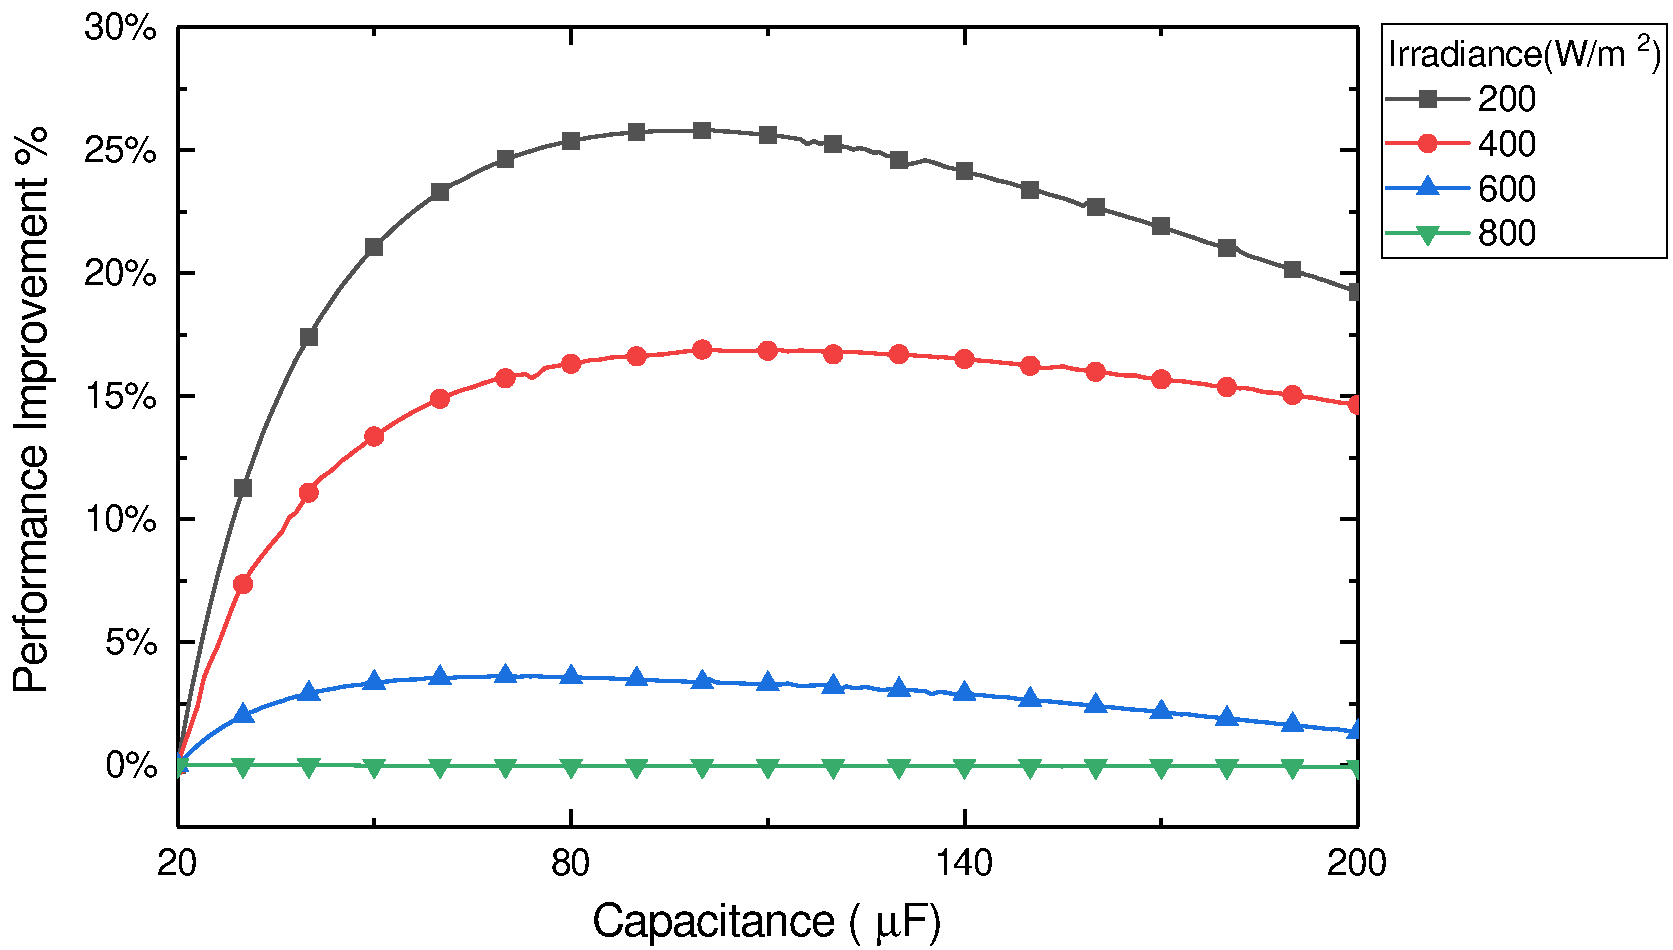
\includegraphics[width=13cm]{figure/work1/VaryCapThrp}
    \caption{Performance improvement (application throughput improvement compared to 20\textmu F capacitance at each energy condition) by increasing capacitance from 20\textmu F to 200\textmu F (at 1\textmu F resolution) given four levels of constant irradiance. }
    \label{Figure:VaryCapThrp}
\end{figure}

To further explain this effect, we investigate a segment of the supply voltage $V_{cc}$ traces at 20\textmu F (minimum performance) and 100\textmu F (maximum performance) under 400$W/m^2$ irradiance (an energy source condition in the Switch region). As shown in Figure \ref{Figure:Vcctrace}, in both traces, $V_{cc}$ experiences discharging and charging intervals periodically. The discharging interval includes resuming execution at $V_{restore}$ = 2.3V and saving state at $V_{save}$ = 2.2V (here, this platform does not need to restore state to resume execution after it wakes up from the sleep mode because this platform keeps volatile state in the sleep mode). In this test, these discharging and charging intervals are periodic because the applied irradiance is constant in these tests. Comparing the 100\textmu F trace to the 20\textmu F one, the increased capacitance prolongs the discharging and charging period, so the save and restore operations are less frequent. The reduction of save and restore operations spares more energy on execution, resulting in higher application throughput. However, increasing capacitance also causes higher leakage, which reduces the amount of usable energy and offsets the improvement gained from increasing storage. This trade-off should be evaluated to find the optimal storage size for maximising performance. 
% starts discharging when reaching the restore threshold ($V_{restore}$ = 2.3V) and triggers saving operation when dropping to the save threshold ($V_{save}$ = 2.2V)

\begin{figure}[H]
    \centering
    \includegraphics[width=13cm]{figure/work1/Vcctrace05-06}
    \caption{Supply Voltage $V_{cc}$ trace segments at 20\textmu F and 100\textmu F under 400$W/m^2$ constant irradiance.}
    \label{Figure:Vcctrace}
\end{figure}

Mathematical equations are developed to abstract this system behaviour and numerically find the trade-off in sizing storage. For covering general cases, a restore operation is included in this analysis between waking up from the sleep mode and resuming execution. 

In one period, the device goes through charging, restoring, executing, and saving intervals sequentially. If we denote $V_{postrestore}$ and $V_{postsave}$ as the voltage after restoring and saving operations, $V_{postrestore}$ and $V_{postsave}$ can be calculated as:

\begin{equation}
    V_{postsave} = V_{save} + \frac{(I_{harvest} - I_{leak} - I_{save}) T_{save}}{C}
    \label{Equation:Vpostsave}
\end{equation}

\begin{equation}
    V_{postrestore} = V_{restore} + \frac{(I_{harvest} - I_{leak} - I_{restore}) T_{restore}}{C}
    \label{Equation:Vpostrestore}
\end{equation}

where $I_{harvest}$, $I_{save}$, and $I_{restore}$ are the average current of harvesting, saving, and restoring in these intervals. If we denote $I_{exe}$ as the average current consumption of execution, the time spent on useful execution $T_{exe}$ can be expressed as:

\begin{equation}
    T_{exe} = \frac{C(V_{postrestore} - V_{save})}{I_{exe} + I_{leak} - I_{harvest}}
    \label{Equation:texe}
\end{equation}

Then, the charging and discharging intervals can be described as:

\begin{equation}
    T_{charge} = \frac{C(V_{restore} - V_{postsave})}{I_{harvest} - I_{leak} - I_{sleep}}
    \label{Equation:tcharge}
\end{equation}

\begin{equation}
    T_{discharge} = T_{restore} + T_{exe} + T_{save}
    \label{Equation:tdischarge}
\end{equation}

Combining Equation \ref{Equation:texe}, \ref{Equation:tcharge}, and \ref{Equation:tdischarge}, we can obtain the percentage of time spent on useful execution:

\begin{equation}
    T_{exe\%} = \frac{T_{exe}}{T_{charge} + T_{discharge}}
\end{equation}

Therefore, the average performance $\overline{S_{app}}$ (represented by application throughput per second) given a constant harvested current in the Switch region can be approximated as:

\begin{equation}
    \overline{S_{app}} = T_{exe\%}\frac{f_{CPU}}{N_{appcycles}}
\end{equation}

where $f_{CPU}$ is the CPU clock frequency, and $N_{appcycles}$ is the number of cycles to complete an application iteration. Here, $\overline{S_{app}}$ can be translated to a function of $C$ and $I_{harvest}$ in the Switch region because all of other parameters are known in parameter settings. After applying the conditions for the Off and On regions (Off: $P_{harvest} < P_{sleep} + P_{leak}$, On: $P_{harvest} > P_{exe} + P_{leak}$), this function for all energy source conditions becomes:

\begin{equation}
    \overline{S_{app}} = f(C, I_{harvest}) = \left\{\begin{aligned}
        & 0 & , & \quad Off \\
        & T_{exe\%} (C, I_{harvest}) \frac{f_{CPU}}{N_{appcycles}} & , & \quad Switch \\
        & \frac{f_{CPU}}{N_{appcycles}} & , & \quad On
    \end{aligned}
    \right.
    \label{Equation:paverage}
\end{equation}

In Equation \ref{Equation:paverage}, we get the relationship between the application performance and the size of energy harvester and storage. $C$ represents the size of the energy storage. $I_{harvest}$ is determined by the energy source condition and the size of the energy harvester. 

We evaluate this theoretical average performance $\overline{S_{app}}$ with our simulation results. An average operating voltage is assumed at $(V_{save} + V_{restore})/2$ to calculate $I_{harvest}$, $I_{exe}$, $I_{sleep}$, $I_{save}$, and $I_{restore}$ in the Switch region. As shown in Figure \ref{Figure:veriTheory}, the theoretical $\overline{S_{app}}$ is compared with simulated $\overline{S_{app}}$ at three energy conditions. The overall mean absolute percentage error (MAPE) is 0.316\%. Therefore, these equations explain the simulation results on performance changes by increasing storage in Figure \ref{Figure:VaryCapThrp}. These equations for estimating the application performance $\overline{S_{app}}$ given constant energy conditions will be used later to estimate $\overline{S_{app}}$ in variable energy conditions. 

% your equations explain what roughly happen in the model/simulation. 
% \dots what does this equation indicate? what cause the change in sizing storage?
% \dots applicable cases. reactive.

\begin{figure}[H]
    \centering
    \begin{subfigure}{0.325\textwidth}
        \centering
        \includegraphics[width=\textwidth]{figure/work1/veriTheory200}
        \caption{Irradiance = 200 $W/m^2$}
    \end{subfigure}
    \begin{subfigure}{0.325\textwidth}
        \centering
        \includegraphics[width=\textwidth]{figure/work1/veriTheory400}
        \caption{Irradiance = 400 $W/m^2$}
    \end{subfigure}
    \begin{subfigure}{0.325\textwidth}
        \centering
        \includegraphics[width=\textwidth]{figure/work1/veriTheory600}
        \caption{Irradiance = 600 $W/m^2$}
    \end{subfigure}
       \caption{Comparison between estimated performance using formulations and simulated performance under constant irradiance.}
       \label{Figure:veriTheory}
\end{figure}

The above analysis indicates that the performance improvement by using larger energy storage is due to reduced saving and restoring overheads in the Switch region, which leads to increased effective computing energy. However, increasing storage also leads to higher leakage consumption. This trade-off is theoretically analysed with mathematical relationships. 

\subsection{Sizing Energy Storage under Real-World Irradiance Conditions} \label{Section:4.3}

We further apply this estimating method for sizing energy storage given real-world energy conditions. 

Real-world energy conditions are time-varying and may cover three operating regions. The previous equations can adapt to time-varying energy conditions by sorting variable energy conditions into time lengths spent on each level of energy condition. To demonstrate this, our method analyses the time distribution of real-world irradiance data, calculates the corresponding performance at each irradiance, and integrate them with time to obtain total throughput (or average performance).

This method is compared with time-based simulation results given monthly irradiance in four different seasons (different amounts of energy sources). As shown in Figure \ref{Figure:CapSizeReal}, an average MAPE is given by 0.892\%. All the four tests shows a maximum performance around 80\textmu F. Comparing the performance at 80\textmu F capacitance to the 20\textmu F one, the performance improvement in the listed tests is 14.5\%, 5.4\%, 4.5\%, and 8.7\% respectively, with an average improvement of 8.3\%.

% \dots how much is the reduction of saving and restoring overhead?

\begin{figure}[H]
    \centering
    \begin{subfigure}{0.49\textwidth}
        \centering
        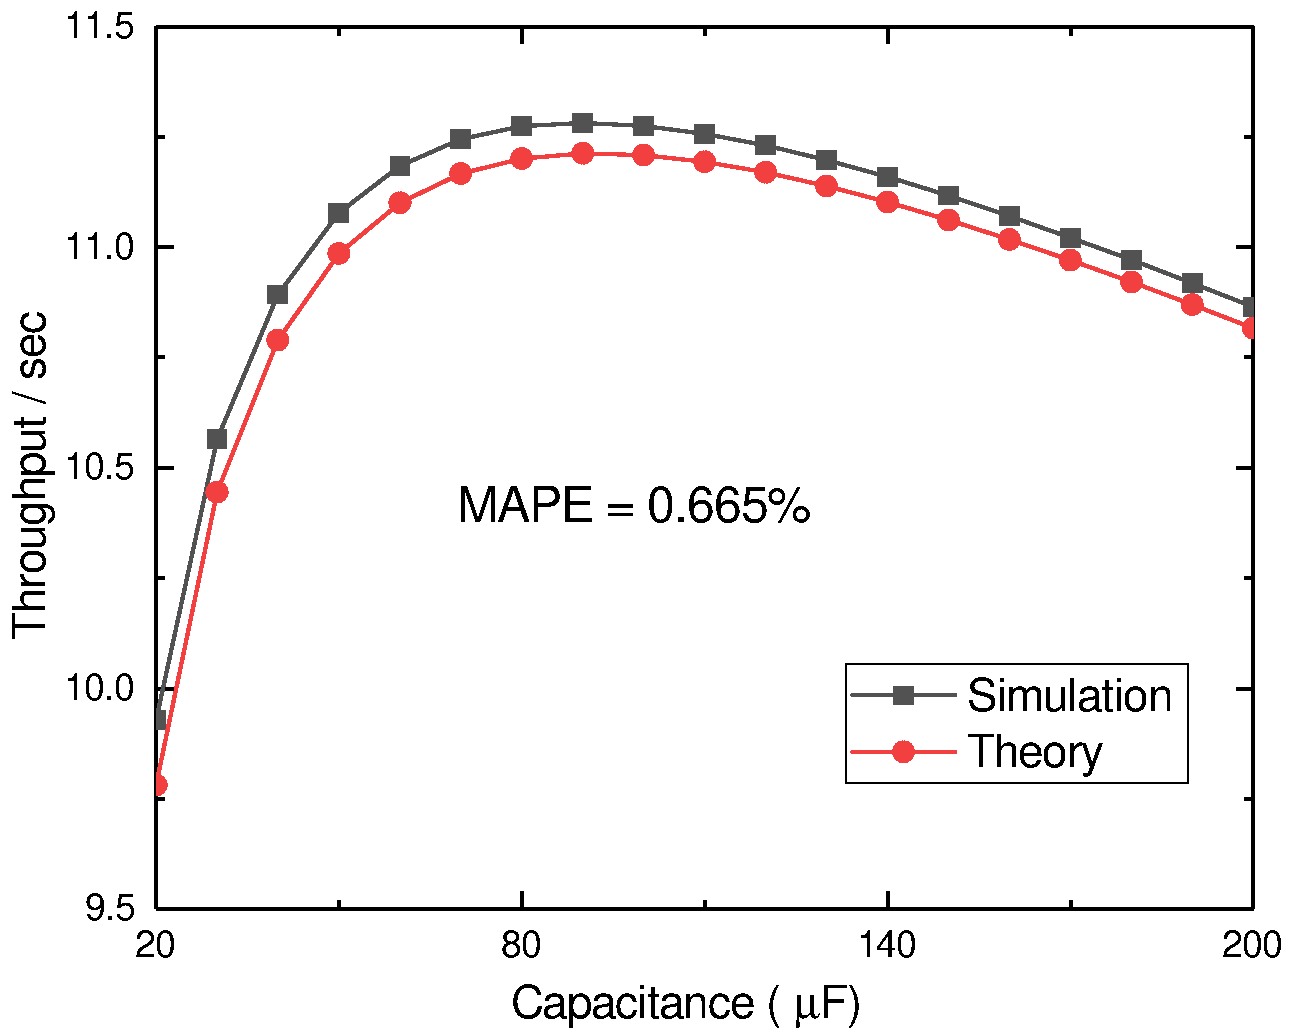
\includegraphics[width=\textwidth]{figure/work1/CapDenvJan}
        \caption{Jan 2018, Denver}
    \end{subfigure}
    \begin{subfigure}{0.49\textwidth}
        \centering
        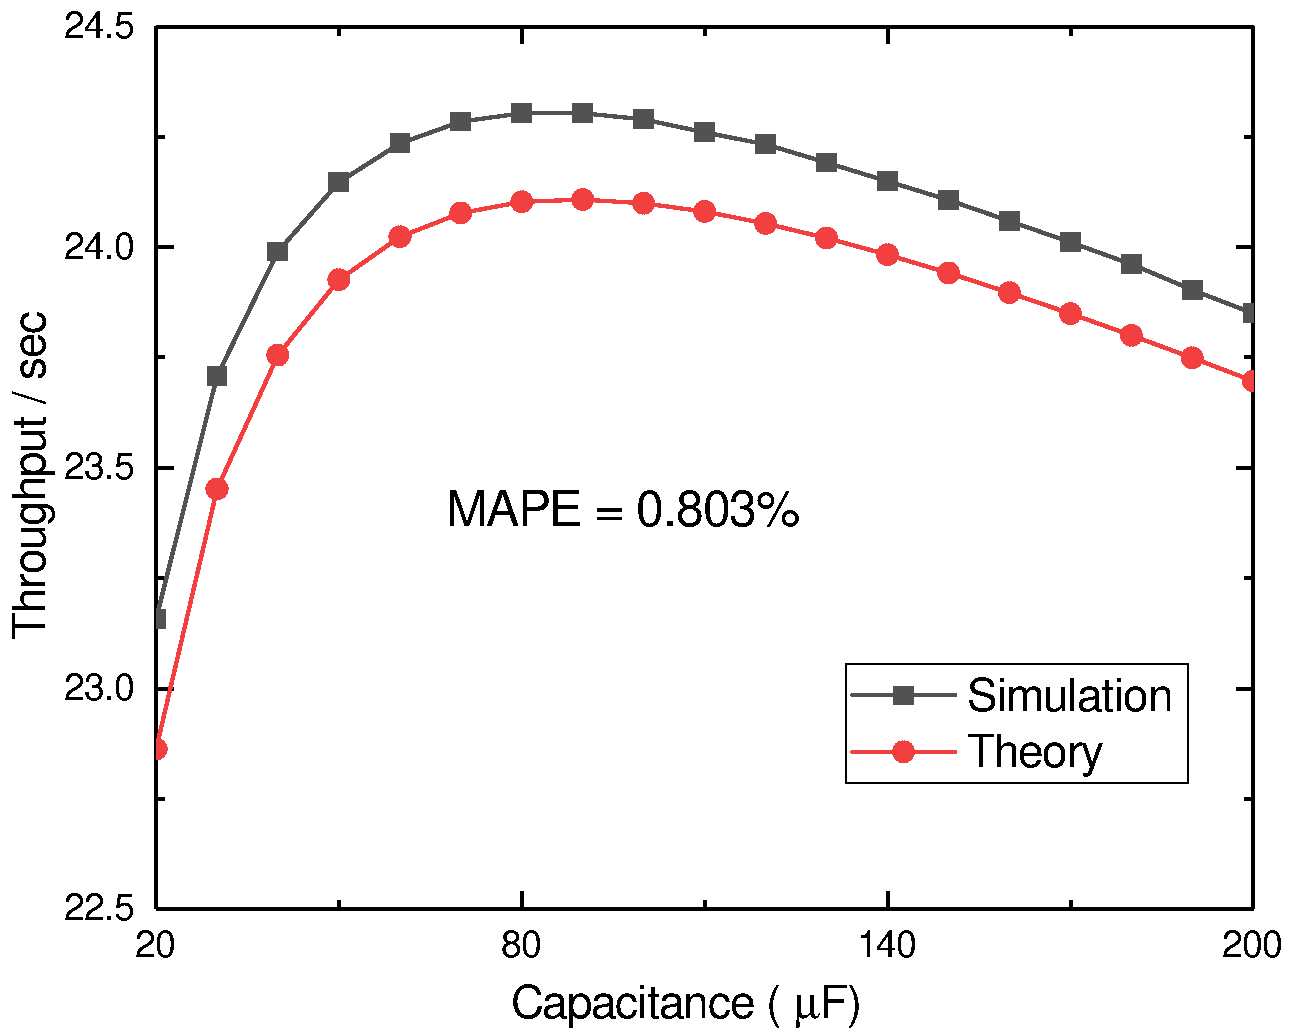
\includegraphics[width=\textwidth]{figure/work1/CapDenvApr}
        \caption{Apr 2018, Denver}
    \end{subfigure}
    \par\bigskip
    \begin{subfigure}{0.49\textwidth}
        \centering
        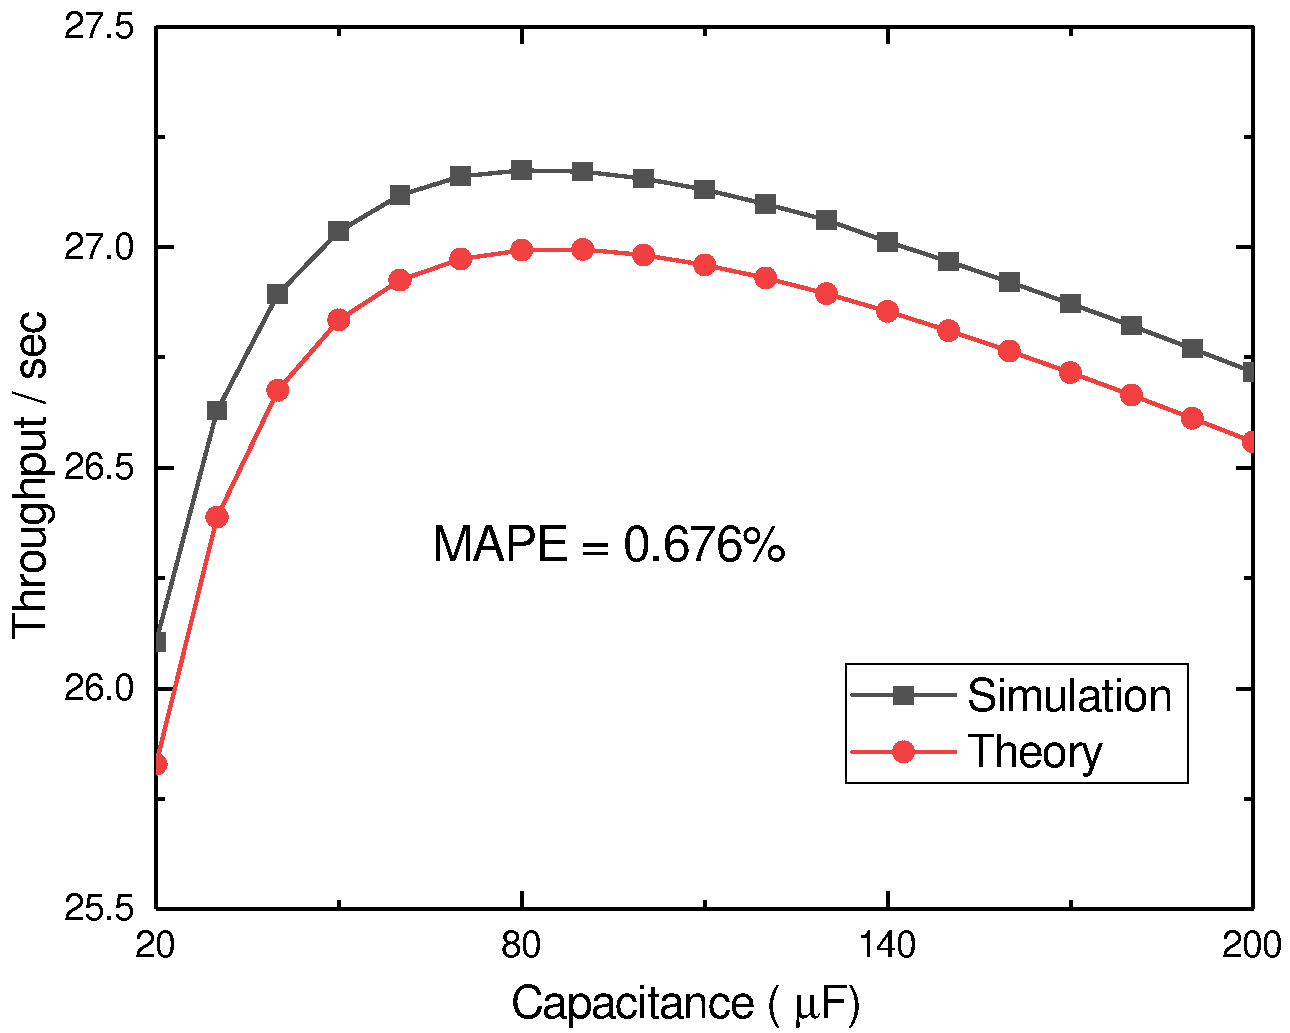
\includegraphics[width=\textwidth]{figure/work1/CapDenvJul}
        \caption{Jul 2018, Denver}
    \end{subfigure}
    \begin{subfigure}{0.49\textwidth}
        \centering
        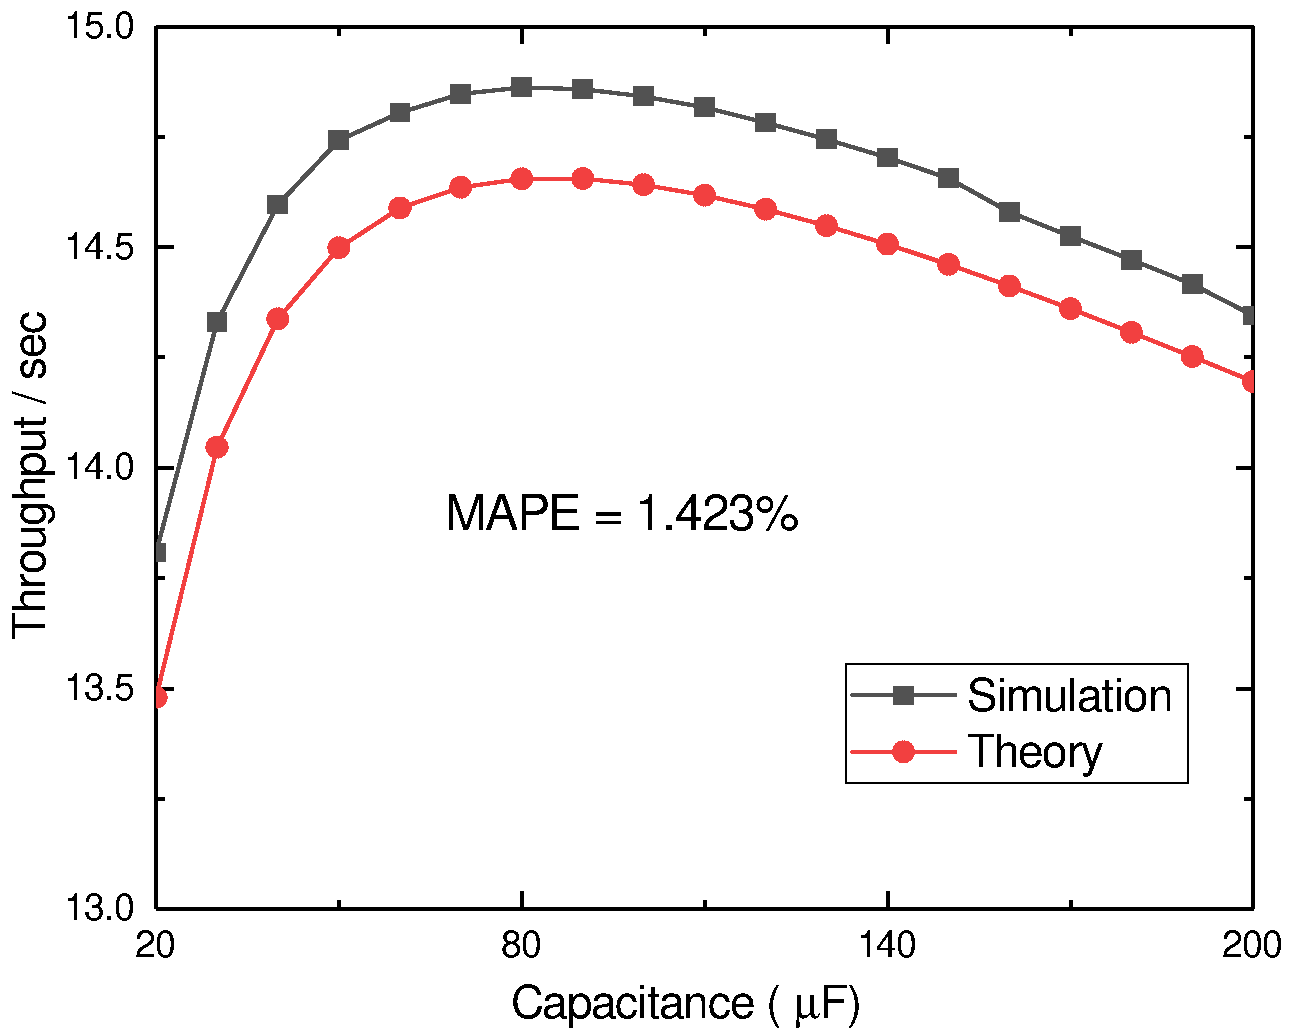
\includegraphics[width=\textwidth]{figure/work1/CapDenvOct}
        \caption{Oct 2018, Denver}
    \end{subfigure}
    \caption{Comparison between estimated and simulated average performance under real-world irradiance data.}
    \label{Figure:CapSizeReal}
\end{figure}
% errors, hysteresis changing between Switch and On

We apply this method to estimate the sizing effect of energy storage on an annual time scale. As shown in Figure \ref{Figure:year2018}, increasing storage from 20\textmu F to 80\textmu F improves the overall throughput by 6.7\% and 5.4\% at the two example locations respectively (given the harvester size used in the prior simulations). However, the system operates in the On region for 10.8\% and 14.6\% of time respectively, which indicates there is excessive power to use. Increasing energy storage cannot make benefit on throughput in the On region, so if the energy conditions are poorer or the harvester size is smaller (where the system spends more time in the Switch region) sizing energy storage will make more improvement. 

\begin{figure}[H]
    \centering
    \begin{subfigure}{0.49\textwidth}
        \centering
        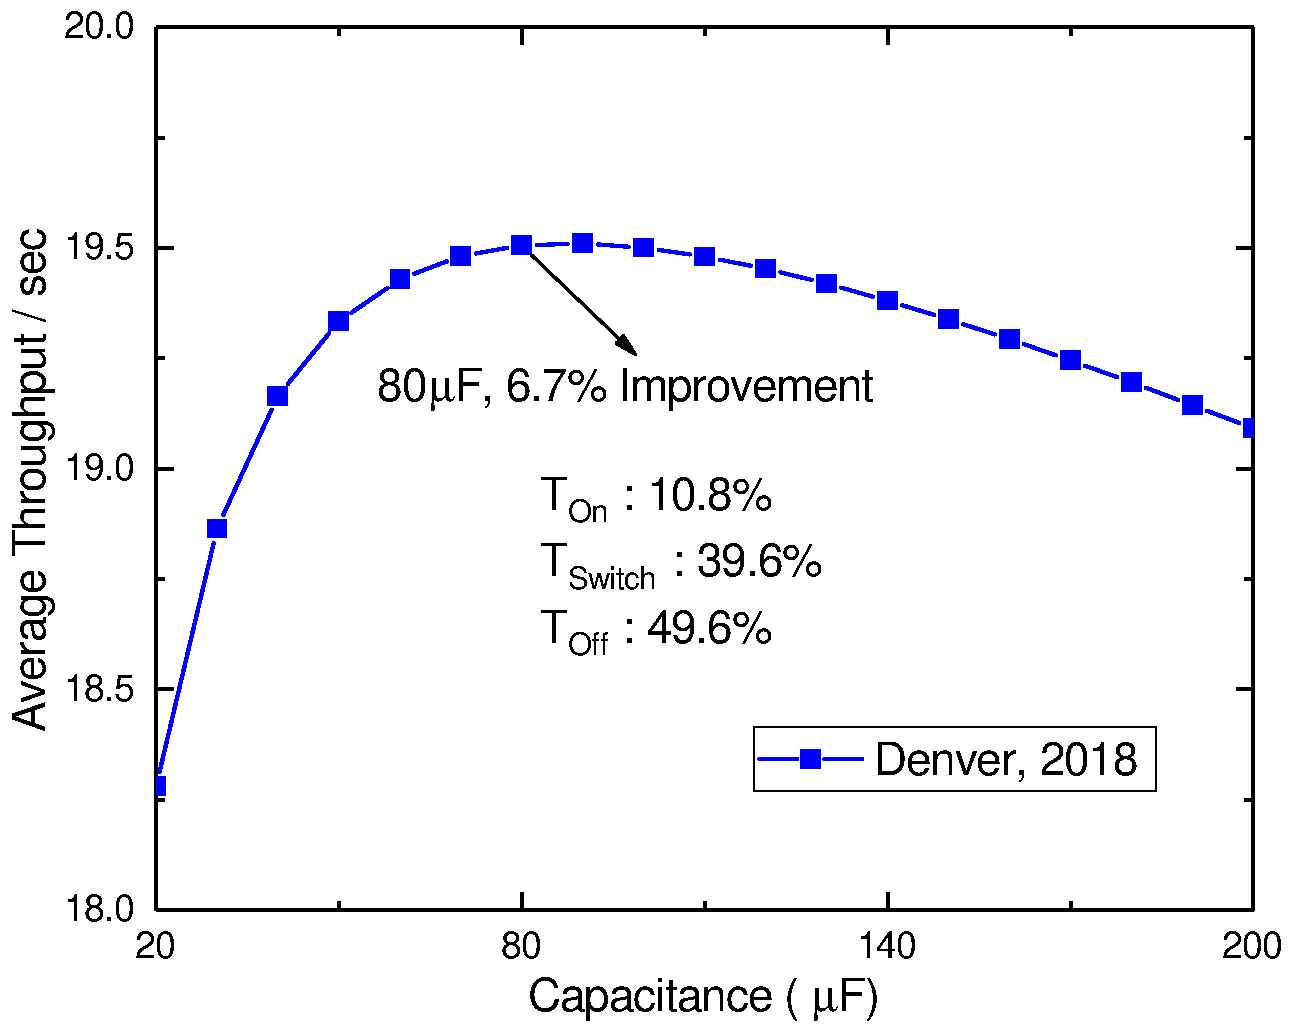
\includegraphics[width=\textwidth]{figure/work1/denver2018}
        \caption{Denver, 2018}
    \end{subfigure}
    \begin{subfigure}{0.49\textwidth}
        \centering
        \includegraphics[width=\textwidth]{figure/work1/hawaii2018}
        \caption{Hawaii, 2018}
    \end{subfigure}
    \caption{Performance estimation given annual solar data, with the time ratio spent on each operating region denoted as $T_{On}$, $T_{Switch}$, and $T_{Off}$.}
    \label{Figure:year2018}
\end{figure}

The dimensions of capacitors varies with its capacity. This capacity-dimension relationship of capacitors is non-linear and largely depends on the packaging methods. A reference for capacitance (in the range discussed) and corresponding dimensions of three example commercial capacitors is listed in Table \ref{Table:capdimension}. Comparing the suggested 80\textmu F capacitor to the minimum 20\textmu F capacitance, which corresponds to 22\textmu F and 82\textmu F capacitors as the nearest available ones in the datasheet of aluminum capacitors, adding this amount of capacitance does not increase the actual dimensions.

\begin{table}[H]
    \caption{Actual dimensions of commercial aluminum and tantalum capacitors with capacitance in the discussed range and 10V rated voltage (D: diameter, L: length, W: width, H: height, unit: millimeters).}
    \label{Table:capdimension}
    \centering
    \begin{tabular}{cccc}
    \toprule
    \textbf{Capacitance} & \textbf{Aluminum} \cite{alcapacitor} & \textbf{Tantalum (Surface Mount)} \cite{tacap1} & \textbf{Tantalum (Dipped Radial Leaded)} \cite{tacap2} \\
    \midrule
    22\textmu F & D5$\times$L11 & L3.2$\times$W1.6$\times$H1.6 & D5.5$\times$L10.5 \\
    33\textmu F & D5$\times$L11 & L3.5$\times$W2.8$\times$H1.9 & D6.0$\times$L11.5 \\
    47\textmu F & D5$\times$L11 & L3.5$\times$W2.8$\times$H1.9 & D6.5$\times$L11.5 \\
    68\textmu F & N/A           & L3.5$\times$W2.8$\times$H1.9 & D7.0$\times$L12.0 \\
    82\textmu F & D5$\times$L11 & N/A                          & N/A \\
    100\textmu F & D5$\times$L11 & L3.5$\times$W2.8$\times$H1.9 & D8.5$\times$L14.0 \\
    120\textmu F & N/A           & L7.3$\times$W4.3$\times$H4.0 & N/A \\
    150\textmu F & D6.3$\times$L11 & L6.0$\times$W3.2$\times$H2.5 & D9.0$\times$L16.0 \\
    220\textmu F & D6.3$\times$L11 & L7.3$\times$W4.3$\times$H2.8 & D10.0$\times$L17.0 \\
    \bottomrule
    \end{tabular}
\end{table}

\subsection{Sizing Energy Harvester under Real-World Irradiance Conditions} \label{Section:4.4}

After exploring the effect of sizing energy storage, we move to explore the effect of sizing energy harvester. Clearly, enlarging energy harvester size, i.e. PV panel area in this case, increases the total amount of harvesting energy, and hence, increases the total application throughput. However, given a certain load deployed under real-world energy conditions, an over-provisioned energy harvester provides more power than the system consumes most of the time. At this point, increasing harvester size makes insignificant improvement on throughput. To evaluate an efficient energy harvester size, we introduce the ratio of the average performance to the energy harvester size (P/S ratio) as a measurement. This measurement indicates how efficiently the harvester size contributes to the application throughput. In our example system powered by PV cells, this measurement corresponds to performance per unit area of PV cells. We will show  that how this measurement varies when scaling the harvester size. 

In Equation \ref{Equation:paverage}, the harvested current $I_{harvest}$ is related to the average performance, and, as mentioned in Section \ref{Section:3.2}, $I_{harvest}$ is proportional to the PV cell area at certain operating voltage and irradiance, so the system performance and the harvester size are linked by $I_{harvest}$. By using the method for performance estimation illustrated in Section \ref{Section:4.2}, an annual average throughput rate is shown in Figure \ref{Figure:SizeHar} with a range of PV panel sizes. To focus on the sizing effect of energy harvester, we avoid sizing energy storage in this test and set the energy storage at 80\textmu F as suggested in the previous simulations. 

\begin{figure}[H]
    \centering
    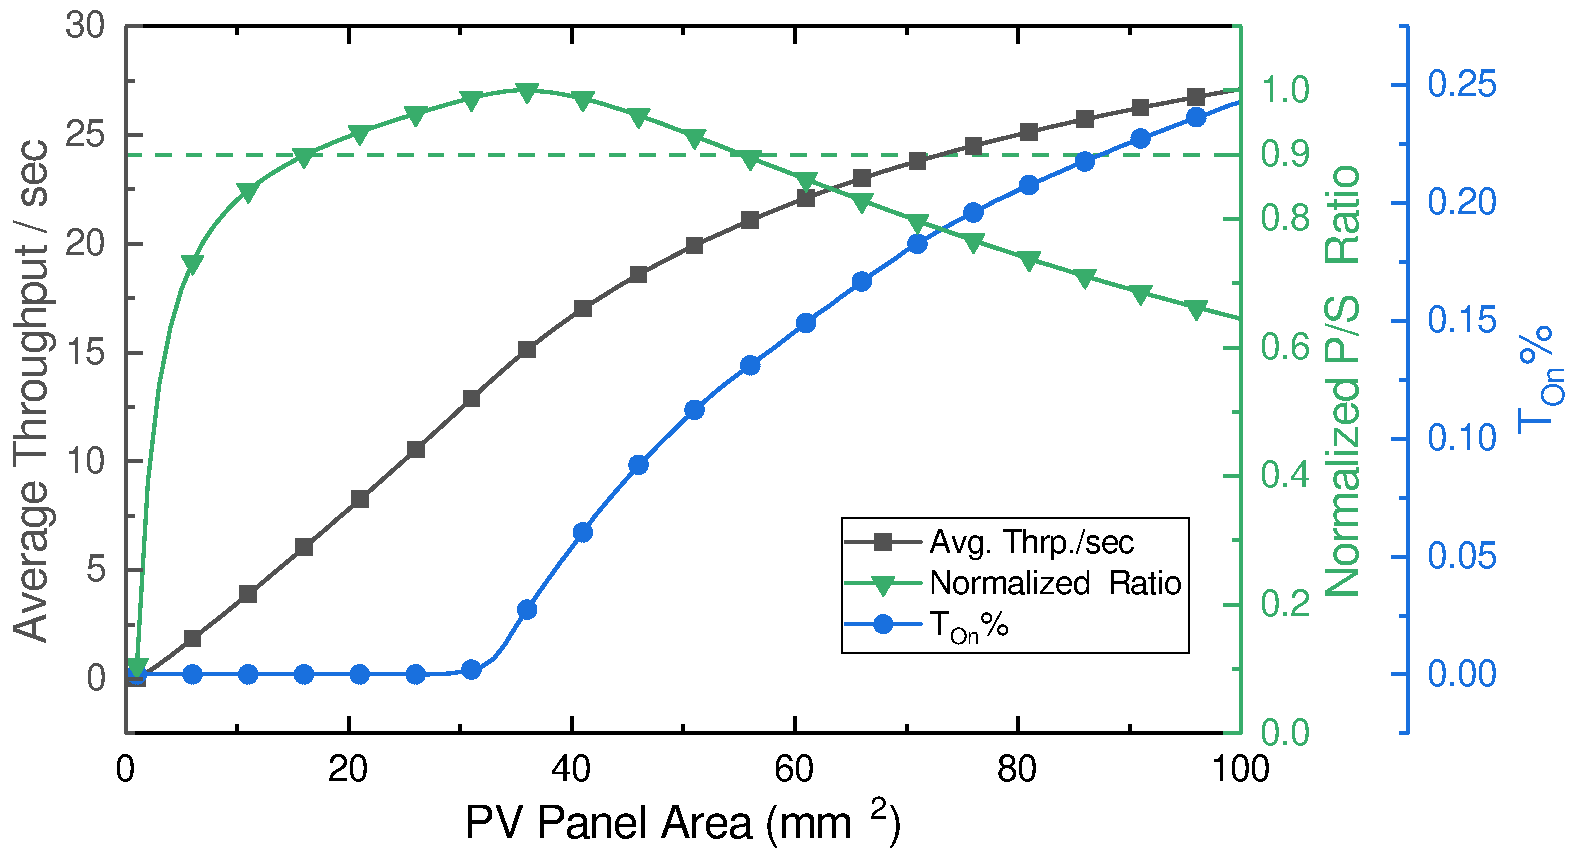
\includegraphics[width=13cm]{figure/work1/SizeHar}
    \caption{Sizing effect of energy harvester given annual outdoor solar irradiance.}
    \label{Figure:SizeHar}
\end{figure}

As shown in Figure \ref{Figure:SizeHar}, the system average performance (throughput per second) increases with the PV panel area, but the relationship is non-linear under real-world varying energy conditions. Given a small harvester (the left end of Figure \ref{Figure:SizeHar}), a large part of the harvested energy is used for compensating the system leakage, so the P/S ratio is low. Given a large harvester (the right end of Figure \ref{Figure:SizeHar}), the system spends nearly 25\% of time in the On region, which means in around half of the daytime the system could have harvested more energy; in this case, enlarging the harvester size is not "profitable". Alternative choices can be using a more powerful load if higher performance is needed or scale down the harvester size if lower performance is still beyond requirement. A harvester size that leads to nearly the maximum P/S ratio is efficient for deploying energy harvesting devices. A reference line of 90\% maximum P/S ratio is given in this figure, and designers can choose a harvester size with P/S ratio above the reference line (from 16mm$^2$ to 56mm$^2$ in this example) according to their needs for minimum performance or maximum area. Nevertheless, harvester sizes outside this range can still be chosen if needed, but that leads to an inefficient harvester deployment. 
% from 18 to 57 mm2

\subsection{Sizing storage and harvester together given real-world irradiance data} \label{Section:4.5}

After explaining the sizing effect of both energy storage and energy harvester, this section presents the combined sizing effect given real-world outdoor solar irradiance as the energy source. As shown in Figure \ref{Figure:SizeHarSto}, the performance is dominated by the energy harvester size because it largely determines how much energy can be generated. For every harvester size shown in this figure, the optimal energy storage size that delivers the best performance occurs at around 80-90\textmu F. This indicates sizing energy storage has little relationship with the energy harvester size. Within a suggested range of efficient energy harvester sizes (from 16$mm^2$ to 56$mm^2$), increasing energy storage to 80\textmu F contributes to 5.7-22.2\% execution speedup. This performance improvement by sizing storage decreases with increased harvester size, because the state management overheads account for a less percentage of the total harvested energy. 

\begin{figure}[H]
    \centering
    \includegraphics[width=13cm]{figure/work1/SizeHarSto}
    \caption{Effect of energy storage and energy harvester sizing on average application performance given yearly outdoor solar irradiance.}
    \label{Figure:SizeHarSto}
\end{figure} 


\section{Discussion}

Although our sizing method considers the distribution of energy conditions after deployment, the variations of energy conditions in the time domain are ignored in this sizing method. Such variations may have an impact on the short-term system behaviours. This impact may not be obvious in solar energy harvesting as the solar source is relatively stable compared to other energy sources, such as radio-frequency signals, human body movements, and acoustic energy. 

Besides the sizing concerns on performance and dimensions discussed above, published works also mention other sizing goals. Colin et al. \cite{Colin:2018:RES:3173162.3173210} propose the need to dynamically scale energy storage at run time to achieve both task atomicity (related to computing correctness in task-based intermittent computing) and execution responsiveness. Also, Jackson \cite{Jackson:2019:COC:3302506.3310400} et al. propose using novel batteries to avoid power intermittency and ensure a high completion rate for periodic workloads.


\section{Summary}

In this chapter, we presented a sizing method for energy storage and energy harvester in energy harvesting IoT deployment, with concerns on device performance and dimensions. We modelled an intermittent computing device based on outdoor solar energy harvesting, with formulations for estimating application performance from harvested power. We analysed the system behaviours of intermittent computing devices and apply our sizing method based on this model. Our sizing method gives a suggestion on energy harvester sizing that balances average performance and device dimensions. Further results show that properly sizing energy storage leads to an execution speedup by 5.7-22.2\% in the suggested range of energy harvester sizes under real-world outdoor deployment. 
% %% ----------------------------------------------------------------
%% CapSizing.tex
%% ----------------------------------------------------------------

\graphicspath{{CapSizing/figure/}}

\chapter{Exploring the Effect of Energy Storage Sizing on Intermittent Computing System Performance}

Batteryless energy-harvesting devices promise to deliver a sustainable Internet of Things. Intermittent computing is an emerging area, where forward progress of application execution is maintained by saving volatile computing state into non-volatile memory before power interruptions, and restored afterwards. Conventional intermittent computing approaches typically minimize energy storage to reduce device dimensions and interruption periods, 
but this can result in high state-saving and -restoring overheads and impede forward progress. 
In this paper, we argue that adding a small amount of energy storage can significantly improve forward progress. 
We develop an intermittent computing model that accurately estimates forward progress, with an experimentally validated mean error of 0.5\%. 
Using this model, we show that sizing energy storage can improve forward progress by up to 65\% with a constant current supply, and 43\% with real-world photovoltaic sources. 

An extension to this approach, which uses a cost function to trade off the energy storage size against forward progress, can save 83\% of capacitor volume and 91\% of interruption periods while maintaining 93\% of the maximum forward progress.

\section{Introduction}

% *** Background of energy harvesting and intermittent systems ***

%Energy harvesting has become a promising power solution for the Internet of Things, liberating wireless sensors from batteries and the power grid~\cite{sliper2020energy-driven}. 
%Batteryless devices harvest ambient energy, such as light, radio-frequency, and mechanical vibration~\cite{sravanthi2008survey, shaikh2016energy}, which is then buffered in a capacitor. 
%As the harvested power is typically insufficient for continuous operation, such devices operate in an intermittent way -- when a certain amount of energy is collected, the processor wakes up, executes program until the amount of energy falls below a threshold, where it sleeps or dies, and waits for the next active cycle\footnote{An active cycle denotes a continuous period that the intermittent system actively executes workloads, i.e. from when it wakes up till it dies or sleeps. }. 
%Prior work in \textit{intermittent systems} has developed sophisticated methods to preserve forward progress across frequent power interruptions by carefully \textit{checkpointing} the volatile computing state in CPU registers and volatile memory into non-volatile memory (NVM), and restoring the state after power interruptions~\cite{umesh2021survey}. 


% *** Previous work on intermittent peripheral operations ***

Apart from computing, embedded sensor systems need to utilize peripherals, such as sensors, computational accelerators, and radios, which typically require \textit{atomicity}~\cite{berthou2020formal}.
In the context of IPSs, an atomic operation should not be checkpointed during execution; if interrupted by power failures, it should restart rather than checkpoint and resume.
% A peripheral operation is considered atomic because it is infeasible to completely read, save, and restore the intermediate internal state of peripherals, and even if possible, could produce unwanted results (e.g. violating timeliness). 
A peripheral operation is considered atomic because it is usually problematic to checkpoint and restore the operation later, even if the intermediate peripheral state is also checkpointed.
For example, checkpointing during a sensor reading and resuming it later can cause incorrect results or an infinite wait as the initialization is lost, and violate timeliness as the sensor does not render the latest and consecutive results~\cite{maeng2019supporting}. 
% disable checkpoints during execution
Prior works on intermittent peripheral operations either customize a design-time calibrated energy budget for each peripheral operation individually~\cite{gomez2016dynamic}, or allocate a universal and large energy budget that ensure the most energy-hungry operation can finish in one active cycle~\cite{maeng2019supporting}.




% *** Offline profiling and fixed threshold is impractical due to variability ***

However, in this paper we argue that manually profiling each peripheral operation and customizing energy thresholds is impractical due to variability in intermittent systems, where we have considered the variability in the data amount to process, peripheral configurations, devices, and energy buffering capacitance (detailed in Section~\ref{subsec:dynamic_energy_consumption}). 
A fixed threshold can be violated if any of the above cases happen, and lead to non-termination\footnote{Non-termination happens when the pre-defined energy budget is less than how much the operation consumes and the supply is not strong enough to fill the energy gap. It is one of the main causes for failures in intermittent systems. }.
In practical deployment, considering the complexity and labour effort, it is unrealistic to profile every atomic operation for every device under every runtime scenario at design time and customize the energy budgets accordingly. 



% *** An optimized threshold improves efficiency ***

On the other hand, using only one high voltage threshold, though probably avoids non-termination, can affect system energy efficiency. 
% Microcontrollers and peripheral devices typically draw more current at a higher supply voltage. 
Intermittent systems typically minimize operating voltage in order to lower quiescent power consumption from power conversion loss and system leakage~\cite{gomez2016dynamic}. 
Also, a high operating voltage can decrease the output current of energy harvesters, making it harder to charge up the buffering capacitor~\cite{pan2017maximize}.
Hence, setting a high wake-up voltage threshold results in a superlinear long charging time, which therefore slows down the system execution or even leave the system in an infinite wait at low input power.
% \todo{Illustrate or demonstrate this?}


% *** What we do to address it ***

To address the above issue, we propose \nn{}\footnote{\nn{}: \underline{O}nline Energy \underline{P}rofiling and \underline{T}hreshold Adaptation for \underline{I}ntermittent \underline{C}omputing Systems. }, a methodology that profiles energy consumption of operations at runtime and dynamically adapts energy thresholds based on newly profiled consumption and user-defined parameters. 
A naive approach of runtime energy profiling can be disconnecting the power supply during profiling and taking two readings of supply voltage before and after an operation~\cite{zhan2020adaptive}, but this can waste the harvested energy during the operation. 
In contrast, \nn{} profiles the maximum drop of supply voltage that an operation can cause while the energy harvesting supply is connected. 
The profiling strategy is to measure the input current in the charging cycle so as to calculate the maximum drop of supply voltage in the discharging cycle. 
The runtime profiled energy budget can closely match the latest energy consumption of an atomic operation. 
Based on the profiling results, \nn{} dynamically adapts the threshold for each atomic operation, with an option of scaling threshold by user-defined parameters or peripheral configurations.
Therefore, \nn{} avoids non-termination and achieves high energy efficiency, improving the workload throughput.

The main contributions of this article are as follows:

\begin{enumerate}
    \item Design exploration (Section~\ref{sec:design_exploration})
    \item Methodology (Section~\ref{sec:method1} and Section~\ref{sec:method2})
    \item Implementation (Section~\ref{sec:implementation})
    \item Experimental evaluation (Section~\ref{sec:experiment})
\end{enumerate}
\input{CapSizing/review2}
%%%%%%%%%%%%%%%%%%%%%%%%%%%%%%%%%%%%%%%%%%%%%%%%%%%%%%%%%%
%%% Section 3: Modelling Reactive
%%%%%%%%%%%%%%%%%%%%%%%%%%%%%%%%%%%%%%%%%%%%%%%%%%%%%%%%%%

\section{Reactive ICS Modelling} \label{section:model}

% The goal of this model is to facilitate making design decisions when deploying intermittent computing devices in real-world environments by enabling designers to observe how the sizes of energy harvester and energy storage have an impact on the key design specifications, i.e. forward progress, dimensions, and interruption periods.

% We then illustrate a formulation which describes the relationship between forward progress and energy storage capacitance given different harvested power level in reactive intermittent computing as a part of the exploration model. 

% Assumptions. low variation in harvested power, how low? what's the impact of high variance input?
% given a constant current supply
To facilitate the understanding and exploration of reactive ICSs, we present a model which outputs the normalized forward progress $\alpha_{exe}$ when powered from a constant current supply $I_{harv}$. Parameters of this model are listed in Table~\ref{tab:parameter}. 
%This accounts for the \textit{Energy Storage} and \textit{Intermittent Load} modules in the system model, allowing the expected forward progress to be evaluated.
% The input parameters $I_{harv}$ and $C$ are related to the size configuration of energy harvester and energy storage respectively. 
% for a period of time that long enough to omit an individual uncompleted operating cycle. 
The model assumes that all configuration parameters remain constant. 

\begin{table}[!t]
    \renewcommand{\arraystretch}{1.2}
    \centering
    \caption{Model parameters of reactive ICS} 
    \label{tab:parameter}
    % Some packages, such as MDW tools, offer better commands for making tables
    % than the plain LaTeX2e tabular which is used here.
    \begin{tabular}{|c|c|}
        % \hline
        % \textbf{Parameter} & \textbf{Description} \\
        \hline
        \multicolumn{2}{|c|}{\textbf{Input Parameters}}\\
        \hline
        $I_{harv}$ & Energy harvester current supply\\
        $C$ & Energy storage capacitance\\
        \hline
        \multicolumn{2}{|c|}{\textbf{Configuration Parameters}}\\
        \hline
        $I_{exe}$ & Execution current draw\\
        $I_{lpm}$ & Low-power mode current draw\\
        %$I_{load}$ & Total current draw of load\\
        $I_{r}$ & Restore current draw\\
        $I_{s}$ & Save current draw\\
        $I_{leak}$ & Leakage current draw\\
        $V_{r}$ & Restore voltage threshold\\
        $V_{s}$ & Save voltage threshold\\
        $T_{r}$ & Restore time overhead\\
        $T_{s}$ & Save time overhead\\
        \hline
        \multicolumn{2}{|c|}{\textbf{Output Parameter}}\\
        \hline
        $\alpha_{exe}$ & Normalized forward progress \\ 
        \hline
    \end{tabular}
\end{table}

% Since supply current $I_{harv}$ and leakage current $I_{leak}$ constantly exist (though could be zero), 
For brevity, $I_{in}$ denotes the usable input current as expressed in (\ref{eq:in}). The effect of capacitor leakage current, $I_{leak}$, is discussed at the end of Section~\ref{subsec:formulation}.
\begin{equation}
  I_{in} = I_{harv} - I_{leak}
  \label{eq:in}
\end{equation}

\subsection{Operating Modes of Reactive ICS}

The behavior of reactive ICSs can be classified into three operating modes depending on the supply current, as shown in \figurename{~\ref{fig:operatingModes}}. These are differentiated by the relationship between input current $I_{in}$ and the system's current draw in its low-power mode (LPM) or active modes, i.e. $I_{lpm}$ and $I_{exe}$. We define the three modes as:

\begin{figure}[!t]
  \centering
  \includegraphics[width=3.2in]{ch3_sizingeffect/figures/OperatingMode0Fig}
  \caption{Operating modes of reactive ICSs, and achieved forward progress against supply current.}
  \label{fig:operatingModes}
\end{figure}

\begin{itemize}
	\item \textit{Off} mode: When $I_{in} < I_{lpm}$, the system stays inactive. The supply voltage $V_{cc}$ cannot rise above the restore threshold $V_{r}$ to wake the system and start execution. The LPM current $I_{lpm}$ includes the consumption of voltage monitoring circuits and system idle current.
	% Here, $I_{lpm}$ is induced after $V_{cc}$ goes above the minimum operating voltage $V_{off}$ where the system waits for $V_{cc}$ to reach $V_{r}$ (when $V_{off} < V_{cc} < V_{R}$). 

    \item \textit{On} mode: When $I_{in} > I_{exe}$, the system executes constantly as the supply voltage $V_{cc}$ never drops below $V_{s}$. $V_{cc}$ grows until $I_{in}$ and $I_{exe}$ are in equilibrium, which may result from $I_{in}$ decreasing due to poor impedance matching, or $I_{exe}$ increasing due to either greater current draw at higher voltage or dissipation through overvoltage protection circuits. 

	\item \textit{Intermittent} mode: When $I_{lpm} < I_{in} < I_{exe}$, the system executes intermittently after $V_{cc} > V_{r}$ and before $V_{cc} < V_{s}$. $V_{cc}$ can rise above $V_{r}$ and the system starts execution. However, the stored energy is then consumed by the load as $I_{in} < I_{exe}$, causing $V_{cc}$ to eventually drop below the save threshold $V_{s}$, where the system saves its state and enters LPM. The system stays in LPM until $V_{cc}$ rises to $V_{r}$ again and then resumes execution. 
	% In this mode, $V_{cc}$ oscillates approximately between $V_{r}$ and $V_{s}$, 'switching' on and off the execution. 
    In general, a higher $I_{in}$ leads to more forward progress in this mode, but the exact relationship between $I_{in}$ and forward progress requires further analysis.
    
	% The excess power either dissipates through circuits or overcharges $V_{cc}$. An overcharged $V_{cc}$ may affect harvesting efficiency due to poor impedance matching and reduce $I_{harv}$, such that current input and consumption are in equilibrium. 
	% In this model case, charging $V_{cc}$ above the maximum power point of the PV cell reduces $I_{harvest}$, and $V_{cc}$ is stable when $I_{harvest} = I_{exe} + I_{leak}$. 
\end{itemize}

\subsection{Formulating Forward Progress} \label{subsec:formulation}

Next, we derive formulations to calculate $\alpha_{exe}$ from $I_{in}$ and energy storage capacitance $C$. We then explore the effect of capacitor leakage on maximum forward progress. 

In the \textit{On} and \textit{Off} modes, the normalized forward progress is trivial to find (simply 1 and 0 respectively). In the \textit{Intermittent} mode,  as shown in \figurename{~\ref{fig:operatingCycle}}, the system goes through four intervals in turn, i.e. charging, restoring, executing, and saving, with current consumption of $I_{lpm}$, $I_{r}$, $I_{exe}$, and $I_{s}$ in each interval respectively. The normalized forward progress, i.e. effective execution time ratio, is indicated as $T_{exe} / T_{cycle}$, where $T_{exe}$ is the time spent on effective execution in one operating cycle and $T_{cycle}$ is the period of operating cycles. Hence, the forward progress given all supply levels is expressed as:
\begin{equation}
    \alpha_{exe} = \left\{
    \begin{aligned}
        & 0 & , & \quad \textit{Off} \, (I_{in} < I_{lpm}) \\
        & \frac{T_{exe}}{T_{cycle}} & , & \quad \textit{Intermittent} \, (I_{lpm} < I_{in} < I_{exe}) \\
        & 1 & , & \quad \textit{On} \, (I_{in} > I_{exe})
    \end{aligned}
    \right.
    \label{eq:feff}
\end{equation}

\begin{figure}[!t]
  \centering
  \includegraphics[width=3.33in]{ch3_sizingeffect/figures/CRESdemoFig}
  \caption{Operating cycles in the \textit{Intermittent} mode. }
  \label{fig:operatingCycle}
\end{figure}

In the following analysis, we focus on deriving $T_{exe} / T_{cycle}$ in the \textit{Intermittent} mode. Let $V_{pr}$ (post-restore) and $V_{ps}$ (post-save) denote the voltage after restoring and saving operations. $V_{pr}$ and $V_{ps}$ can be calculated as:
\begin{equation}
  V_{pr} = V_{r} + \frac{T_{r} (I_{in} - I_{r})}{C}
  \label{eq:vpr}
\end{equation}
\begin{equation}
  V_{ps} = V_{s} + \frac{T_{s} (I_{in} - I_{s})}{C}
  \label{eq:vps}
\end{equation}
With (\ref{eq:vpr}), the time spent on effective execution $T_{exe}$ in one operating cycle can be expressed as:
\begin{equation}
%   \begin{aligned}
    T_{exe} = \frac{C(V_{pr} - V_{s})}{I_{exe} - I_{in}} 
    % & = \frac{C(V_{r} - V_{s}) + T_{r} (I_{in} - I_{r})} {I_{exe} - I_{in}}
%   \end{aligned}
  \label{eq:texe}
\end{equation}
Analogously, with (\ref{eq:vps}), the charging interval can be described as:
\begin{equation}
%   \begin{aligned}
    T_{charge} = \frac{C(V_{r} - V_{ps})}{I_{in} - I_{lpm}}
    % & = \frac{C(V_{r} - V_{s}) - T_{s} (I_{in} - I_{s})} {I_{in} - I_{lpm}}
%   \end{aligned}
  \label{eq:tcharge}
\end{equation}
With (\ref{eq:texe}) and (\ref{eq:tcharge}), the period of an operating cycle is:
\begin{equation}
%   \begin{aligned}
    T_{cycle} = \quad T_{charge} + T_{r} + T_{exe} + T_{s} 
%     = & \quad \frac{C (V_{r} - V_{s}) + T_{s} (I_{s} - I_{lpm})}{I_{in} - I_{lpm}} \quad + \\
%     & \quad \frac{C (V_{r} - V_{s}) + T_{r} (I_{exe} - I_{r})}{I_{exe} - I_{in}}
%   \end{aligned}
  \label{eq:tperiod}
\end{equation}

Finally, combining (\ref{eq:vpr})--(\ref{eq:tperiod}), we obtain normalized forward progress $\alpha_{exe}$ in the \textit{Intermittent} mode as:
\begin{equation}
    \begin{aligned}
        \alpha_{exe} &= \frac{T_{exe}}{T_{cycle}} \\ %, \quad I_{lpm} < I_{in} < I_{exe}
                     &= \frac{\frac{C (V_{r} - V_{s}) + T_{r} (I_{in} - I_{r})} {I_{exe} - I_{in}}}{\quad \frac{C (V_{r} - V_{s}) + T_{s} (I_{s} - I_{lpm})}{I_{in} - I_{lpm}} + \frac{C (V_{r} - V_{s}) + T_{r} (I_{exe} - I_{r})}{I_{exe} - I_{in}}} \\
                    %  &= \frac{\scriptstyle \bigl[C (V_{r} - V_{s}) + T_{r} (I_{in} - I_{r}) \bigr] (I_{in} - I_{lpm})}{\scriptscriptstyle C (V_{r} - V_{s}) (I_{exe} - I_{lpm}) + T_{s} (I_{in} - I_{s}) (I_{exe} - I_{in}) + T_{r} (I_{exe} - I_{r}) (I_{in} - I_{lpm})} \\
    \end{aligned}
    \label{eq:texepercent}
\end{equation}
In the numerator $T_{exe}$, $C(V_{r} - V_{s})$ represents the amount of charge in the capacitor available for restoring and executing. $T_{r} (I_{in} - I_{r})$ represents the charge used by a restore operation. $I_{exe} - I_{in}$ is the rate of charge consumption from the energy storage during execution.

% \footnote{Calculation breakdowns of differential analysis is attached in Appendix.}
% Higher $\alpha_{exe}$ leads to more time spent on forward progress. 

% As $d\alpha_{exe} / dI_{in}$ is positive, higher harvested current $I_{harv}$ leads to more forward progress. 
To explore the effect of energy storage on forward progress, we need to analyze $d\alpha_{exe} / dC$. Here, if we assume that $I_{leak}$ remains constant, $\alpha_{exe}$ keeps increasing and approaches $(I_{in} - I_{lpm}) / (I_{exe} - I_{lpm})$ when energy storage capacitance $C$ increases. Defining $(I_{in} - I_{lpm}) / (I_{exe} - I_{lpm})$ as $\alpha_{exe\_ideal}$, $\alpha_{exe} = \alpha_{exe\_ideal}$ is an ideal case, where restore and save overheads are absent.

In an electrolytic capacitor, however, $I_{leak}$ typically increases with $C$ with the following relationship~\cite{avxleakage}:
\begin{equation}
    I_{leak} = kCV_{cc}
    \label{eq:ileak}
\end{equation}
where $k$ is a constant normally in a range 0.01 to 0.03 ($\frac{A}{F \cdot V}$). Combining (\ref{eq:ileak}) with (\ref{eq:in}), $dI_{in} / dC$ is $-kV_{cc}$, meaning $I_{in}$ decreases linearly as $C$ increases. Thus, when $C$ increases, $\alpha_{exe}$ keeps approaching $\alpha_{exe\_ideal}$ while $\alpha_{exe\_ideal}$ decreases. Hence, we believe that there is a capacitance value that leads to the maximum $\alpha_{exe}$ considering $I_{leak}$ increases with $C$.
% \cite{alcapacitor}
% Also, the time overhead of state saving and restoring operations $T_{RS\%}$ can be calculated as:
% \begin{equation}
%   T_{RS\%} = \frac{T_{R} + T_{S}}{T_{exe} + T_{R} + T_{S}}
% \end{equation}


% In Equation~(\ref{eq:feff}), we get the relationship between forward progress and the sizes of energy harvester and energy storage. 

\section{Experimental Evaluation} \label{sec:experiment}

We experimentally evaluated \nn{}, showing its ability to run with an adaptive minimum threshold that mitigate non-termination and improve energy efficiency. 
\nn{}'s runtime energy profiling presents a low and relatively consistent error across different task scales. 
We show that, despite with reduced capacitance, \nn{} is able to adapt \nm{V}{th} to meet a target end voltage \nm{V}{end} until the highest threshold is reached, while the fixed-threshold comparison \debs{} fails.
We also show that \nn{} improves performance over \debs{} and Samoyed with a PV panel supply owning to its reduced operating voltage. 

\subsection{Experimental Setup and Benchmarks}

A PV panel (Sanyo AM-1417CA) provided the sole power supply for the system. 
It is covered in a black box with a white LED light as the only energy source, producing a consistent supply characteristic (as shown in \fref{fig:pv_iv}) during the experiments.
For the experiment on capacitance reduction only, we instead use a constant low-current supply so as to examine whether the system is able to survive with little energy income during task execution. 

Three common peripheral tasks in IoT sensors were used as the benchmarks for evaluation. 
\begin{itemize}
    \item \textbf{DMA}: Data transfer using an on-chip DMA module, frequently used in data logging.
    \item \textbf{AES}: AES encryption using an on-chip AES accelerator processing up to 4KB data at a time for secure communication.
    \item \textbf{RF}:  Wireless communication through an external nRF24L01 radio module, transmitting a payload up to 96B at a time, configured as a 2Mbps air data rate and a \SI{0}{\decibel{m}} output power. 
    The radio module is connected through an LDO with a \SI{2}{\volt} output voltage to lower the quiescent current consumption, with a \SI{10}{\micro\farad} at the LDO's low side. 
\end{itemize}

% No state retention

% Comparisons: DEBS, Samoyed (without scaling), Plain C (for evaluating overheads)
% Samoyed scales down the atomic task if it fails to complete (but never scales back). 
% It uses an "energy profiler" in previous work to test the whether the smallest scale of all peripheral tasks and randomised inputs can successfully complete. 
% They suggested it is appropriate to set an energy capacity that can run the smallest scale of an operation for hundreds of times in one active cycle. 
% Hence, it does not look for a threshold for a task with a specific configuration, but instead its aim is to minimise the chance of non-termination in practice by giving a high margin.

\subsection{Profiling Accuracy}
% Question: How does our profiling approach perform in terms of accuracy?
% Accuracy compared to manual measurement.

\begin{figure*}[t]
    \centering
    \begin{tikzpicture}
    \begin{groupplot}[
        group style={group size=3 by 1},
        width=0.73\columnwidth, height=4cm,
        xmin=-15,xmax=15,
        ymin=0,ymax=100,
        xtick distance=5,
        xticklabel pos=bottom,
        yticklabel={\pgfmathprintnumber\tick\%},
        every tick label/.append style={font=\small},
        minor x tick num=0,
        area style,
        xlabel={Error (\SI{}{\milli\volt})},
        xlabel style={yshift=3pt,},
        title style={at={(0.5,0)},anchor=north,yshift=-1cm},
        ]

        \nextgroupplot [title={(a) DMA}]
        \addplot 
            plot [ybar interval,mark=no,black,fill=Set1-B,]
            table [x=v_error,y=repa_dma,col sep=comma] {ch5_optic/figures/profiling_accuracy/profiling_accuracy.csv};
        \node (n1) at (axis cs:0,100) {};
        \node (n2) at (axis cs:0,0) {};
        \draw [color=Set1-A,ultra thick,dashed] (n2) -- (n1);
        \node [anchor=north east, font=\footnotesize, color=Set1-A] at (axis cs:0,97) {$\Delta V_{\text{task}}$=\SI{107}{\milli\volt}};

        \nextgroupplot [title={(b) AES}]
        \addplot 
            plot [ybar interval,mark=no,black,fill=Set1-B,]
            table [x=v_error,y=repa_aes,col sep=comma] {ch5_optic/figures/profiling_accuracy/profiling_accuracy.csv};
        \node (n1) at (axis cs:0,100) {};
        \node (n2) at (axis cs:0,0) {};
        \draw [color=Set1-A,ultra thick,dashed] (n2) -- (n1);
        \node [anchor=north east, font=\footnotesize, color=Set1-A] at (axis cs:0,97) {$\Delta V_{\text{task}}$=\SI{583}{\milli\volt}};

        \nextgroupplot [title={(c) RF}]
        \addplot 
            plot [ybar interval,mark=no,black,fill=Set1-B,]
            table [x=v_error,y=repa_radio,col sep=comma] {ch5_optic/figures/profiling_accuracy/profiling_accuracy.csv};
        \node (n1) at (axis cs:0,100) {};
        \node (n2) at (axis cs:0,0) {};
        \draw [color=Set1-A,ultra thick,dashed] (n2) -- (n1);
        \node [anchor=north east, font=\footnotesize, color=Set1-A] at (axis cs:0,97) {$\Delta V_{\text{task}}$=\SI{720}{\milli\volt}};
    \end{groupplot}
    \end{tikzpicture}
    \caption{\nn{} Profiling accuracy. }
    \label{fig:profiling_accuracy}
\end{figure*} 

% % Old figure
% \begin{figure*}[t]
%     \centering
%     \begin{tikzpicture}
%     \begin{groupplot}[
%         group style={group size=3 by 2, vertical sep=43pt},
%         width=0.7\columnwidth, height=3.7cm,
%         xmin=-15,xmax=15,
%         ymin=0,ymax=100,
%         xtick distance=5,
%         % xtick pos=top,
%         xticklabel pos=bottom,
%         yticklabel={\pgfmathprintnumber\tick\%},
%         every tick label/.append style={font=\small},
%         minor x tick num=0,
%         area style,
%         xlabel={Error (\SI{}{\milli\volt})},
%         xlabel style={yshift=3pt,},
%         title style={yshift=-7pt,},
%         ]

%         \nextgroupplot [title={(a) REPA, DMA Transfer}]
%         \addplot 
%             plot [ybar interval,mark=no,black,fill=Set1-B,]
%             table [x=v_error,y=repa_dma,col sep=comma] {figures/profiling_accuracy/profiling_accuracy.csv};
%         \node [anchor=north, font=\footnotesize, color=Set1-A] (n1) at (axis cs:0,100) {\SI{107}{\milli\volt}};
%         \node (n2) at (axis cs:0,0) {};
%         \draw [color=Set1-A,thick,dashed] (n2) -- (n1);

%         \nextgroupplot [title={(b) REPA, AES Encryption}]
%         \addplot 
%             plot [ybar interval,mark=no,black,fill=Set1-B,]
%             table [x=v_error,y=repa_aes,col sep=comma] {figures/profiling_accuracy/profiling_accuracy.csv};
%         \node [anchor=north, font=\footnotesize, color=Set1-A] (n1) at (axis cs:0,100) {\SI{583}{\milli\volt}};
%         \node (n2) at (axis cs:0,0) {};
%         \draw [color=Set1-A,thick,dashed] (n2) -- (n1);

%         \nextgroupplot [title={(c) REPA, Radio Transmission}]
%         \addplot 
%             plot [ybar interval,mark=no,black,fill=Set1-B,]
%             table [x=v_error,y=repa_radio,col sep=comma] {figures/profiling_accuracy/profiling_accuracy.csv};
%         \node [anchor=north, font=\footnotesize, color=Set1-A] (n1) at (axis cs:0,100) {\SI{720}{\milli\volt}};
%         \node (n2) at (axis cs:0,0) {};
%         \draw [color=Set1-A,thick,dashed] (n2) -- (n1);

%         \nextgroupplot [title={(d) Naive, DMA Transfer}]
%         \addplot 
%             plot [ybar interval,mark=no,black,fill=Set1-B,]
%             table [x=v_error,y=naive_dma,col sep=comma] {figures/profiling_accuracy/profiling_accuracy.csv};
%         \node [anchor=north, font=\footnotesize, color=Set1-A] (n1) at (axis cs:0,100) {\SI{107}{\milli\volt}};
%         \node (n2) at (axis cs:0,0) {};
%         \draw [color=Set1-A,thick,dashed] (n2) -- (n1);

%         \nextgroupplot [title={(e) Naive, AES Encryption}]
%         \addplot 
%             plot [ybar interval,mark=no,black,fill=Set1-B,]
%             table [x=v_error,y=naive_aes,col sep=comma] {figures/profiling_accuracy/profiling_accuracy.csv};
%         \node [anchor=north, font=\footnotesize, color=Set1-A] (n1) at (axis cs:0,100) {\SI{583}{\milli\volt}};
%         \node (n2) at (axis cs:0,0) {};
%         \draw [color=Set1-A,thick,dashed] (n2) -- (n1);

%         \nextgroupplot [title={(f) Naive, Radio Transmission}]
%         \addplot 
%             plot [ybar interval,mark=no,black,fill=Set1-B,]
%             table [x=v_error,y=naive_radio,col sep=comma] {figures/profiling_accuracy/profiling_accuracy.csv};
%         \node [anchor=north, font=\footnotesize, color=Set1-A] (n1) at (axis cs:0,100) {\SI{720}{\milli\volt}};
%         \node (n2) at (axis cs:0,0) {};
%         \draw [color=Set1-A,thick,dashed] (n2) -- (n1);
        
%     \end{groupplot}


%     \end{tikzpicture}
%     \caption{Profiling accuracy. }
%     \label{fig:profiling_accuracy}
% \end{figure*} 


\todo[inline]{Should present Figure 5.9 with a smaller division.}

We first measured the profiling accuracy of \nn{}'s runtime energy profiling ability. 
A hundred profiling results were obtained for each workload. 
Manual profiling was also conducted by disconnecting the power supply during task execution and reading $\Delta\nmm{V}{task}$ from a scope, and used as a reference that we evaluate the profiling results against. 
As shown in \fref{fig:profiling_accuracy}, the profiling errors are low and relatively consistent (mostly within \SI{5}{\milli\volt}) across the three workload with different levels of energy consumption. 
The error becomes insignificant with energy-hungry tasks, e.g. RF. 
Compared to the step of voltage thresholds in our implementation (around \SI{30}{\milli\volt}), this \SI{5}{\milli\volt} error is acceptable as it can convert to a relatively stable threshold assuming a fixed energy consumption. 
Additionally, the average profiling results are shown to be a slightly higher than the reference, which 
seems to contradict the theoretical error that is supposed to make the profiling undershoot.
This is majorly due to a positive error in the MCU's internal 1/2 \nm{V}{cc} divider, which also evidences that the theoretical error is insignificant and easily compensated by other factors. 

\todo[inline]{Energy saving compared to the disconnect-supply profiling method?}

\subsection{Reliability with Dynamic Energy Consumption}

Question: Can it still make forward progress correctly with changes (as listed below) while other SoA approaches can't? 

New categories:

\begin{itemize}
    \item Changing once: new operations, device/components variability (including capacitor tolerance).
    \item Changing slowly: capacitor ageing, device ageing, temperature, long-term configuration.
    \item Changing frequently: Data size, configurations. 
\end{itemize}

\subsubsection{New devices / operations (once)}

\begin{figure}
    \centering
    \includegraphics[width=\columnwidth]{ch5_optic/figures/v_trace/v_trace.pdf}
    \caption{Voltage trace. }
    \label{fig:v_trace}
\end{figure}

- Show the voltage trace that illustrates how it profiles and adapts on new devices or new operations. 

\subsubsection{Variability in capacitance due to ageing / tolerance (slowly changing)}


% \begin{figure*}[t]
%     \centering
%     \begin{tikzpicture}
%     \begin{groupplot}[
%         group style={group size=1 by 2,vertical sep=2pt},
%         width=0.5\columnwidth,
%         xmin=0,xmax=80,
%         every tick label/.append style={font=\small},
%         minor x tick num=0,
%         ]

%         % (a) upper
%         \nextgroupplot[
%             const plot,
%             height=4cm,
%             ymin=-0.2,ymax=1.2,
%             ytick distance=1,
%             xticklabel=\empty,
%             yticklabels={,Fail,Done},
%             legend style={
%                 anchor=west,
%                 at={(0.02,0.5)},
%                 font=\footnotesize,
%                 legend columns=2,
%             },
%             ]
%         \addplot 
%             plot [Set1-B,mark=o]
%             table [x=cap_reduction,y=opta_perf,col sep=comma] {ch5_optic/figures/capacitance/cap_test_dma.csv};
%         \addplot 
%             plot [Set1-A,mark=square]
%             table [x=cap_reduction,y=debs_perf,col sep=comma] {ch5_optic/figures/capacitance/cap_test_dma.csv};
%         \legend{\nn{},\debs{}}

%         % (b) upper
%         \nextgroupplot[
%             const plot,
%             height=4cm,
%             ymin=-0.2,ymax=1.2,
%             ytick distance=1,
%             xticklabel=\empty,
%             yticklabels={,Fail,Done},
%             legend style={
%                 anchor=west,
%                 at={(0,0.5)},
%                 font=\footnotesize,
%                 legend columns=2,
%             },
%             ]
%         \addplot 
%             plot [Set1-B,mark=o]
%             table [x=cap_reduction,y=opta_perf,col sep=comma] {ch5_optic/figures/capacitance/cap_test_aes.csv};
%         \addplot 
%             plot [Set1-A,mark=square]
%             table [x=cap_reduction,y=debs_perf,col sep=comma] {ch5_optic/figures/capacitance/cap_test_aes.csv};
%         % \legend{\nn{},\debs{}}

%         % (a) lower
%         \nextgroupplot[
%             height=6cm,
%             title={(a) DMA},
%             title style={at={(0.5,0)},anchor=north,yshift=-30pt,},
%             ymin=1.7,ymax=2.5,
%             xlabel={Capacitance Reduction},
%             ylabel={Start \& End Voltage (V)},
%             ytick distance=0.2,
%             xlabel style={yshift=3pt,},
%             xticklabel={\pgfmathprintnumber\tick\%},
%             legend style={
%                 anchor=north west,
%                 at={(0.02,0.98)},
%                 font=\footnotesize,
%                 legend columns=2,
%             },
%             ]
%         \addplot 
%             plot [Set1-B,mark=*]
%             table [x=cap_reduction,y=opta_v_start,col sep=comma] {ch5_optic/figures/capacitance/cap_test_dma.csv};
%         \addplot 
%             plot [Set1-B,mark=o]
%             table [x=cap_reduction,y=opta_v_end,col sep=comma] {ch5_optic/figures/capacitance/cap_test_dma.csv};
%         \addplot 
%             plot [Set1-A,mark=square*]
%             table [x=cap_reduction,y=debs_v_start,col sep=comma] {ch5_optic/figures/capacitance/cap_test_dma.csv};
%         \addplot 
%             plot [Set1-A,mark=square]
%             table [x=cap_reduction,y=debs_v_end,col sep=comma] {ch5_optic/figures/capacitance/cap_test_dma.csv};
%         \draw [thick,dashed] (axis cs:0,2) -- (axis cs:80,2);
%         \node [anchor=north east,font=\small] at (axis cs:80,2) {Target $V_{\text{end}}$};
%         \draw [thick,dashed] (axis cs:0,1.8) -- (axis cs:80,1.8);
%         \node [anchor=north east,font=\small] at (axis cs:80,1.8) {Fail};
%         \legend{\ ,\nn{} $V_{\text{start}}\ V_{\text{end}}$,\ ,\debs{} $V_{\text{start}}\ V_{\text{end}}$}

%         % (b) lower
%         \nextgroupplot[
%             height=6cm,
%             title={(b) AES},
%             title style={at={(0.5,0)},anchor=north,yshift=-30pt,},
%             ymin=1.55,ymax=3.7,
%             xlabel={Capacitance Reduction},
%             ytick distance=0.5,
%             extra y ticks={1.8},
%             xlabel style={yshift=3pt,},
%             xticklabel={\pgfmathprintnumber\tick\%},
%             legend style={
%                 anchor=north west,
%                 at={(0,1)},
%                 font=\footnotesize,
%                 legend columns=2,
%             },
%             ]
%         \addplot 
%             plot [Set1-B,mark=*]
%             table [x=cap_reduction,y=opta_v_start,col sep=comma] {ch5_optic/figures/capacitance/cap_test_aes.csv};
%         \addplot 
%             plot [Set1-B,mark=o]
%             table [x=cap_reduction,y=opta_v_end,col sep=comma] {ch5_optic/figures/capacitance/cap_test_aes.csv};
%         \addplot 
%             plot [Set1-A,mark=square*]
%             table [x=cap_reduction,y=debs_v_start,col sep=comma] {ch5_optic/figures/capacitance/cap_test_aes.csv};
%         \addplot 
%             plot [Set1-A,mark=square]
%             table [x=cap_reduction,y=debs_v_end,col sep=comma] {ch5_optic/figures/capacitance/cap_test_aes.csv};
%         \draw [thick,dashed] (axis cs:0,2) -- (axis cs:80,2);
%         \node [anchor=south east,font=\small] at (axis cs:80,2) {Target $V_{\text{end}}$};
%         \draw [thick,dashed] (axis cs:0,1.8) -- (axis cs:80,1.8);
%         \node [anchor=north east,font=\small] at (axis cs:80,1.8) {Fail};
%         % \legend{\ ,\nn{} $V_{\text{start}}\ V_{\text{end}}$,\ ,\debs{} $V_{\text{start}}\ V_{\text{end}}$}

%         % (c) upper
%         \nextgroupplot[
%             const plot,
%             height=4cm,
%             ymin=-0.2,ymax=1.2,
%             ytick distance=1,
%             xticklabel=\empty,
%             yticklabels={,Fail,Done},
%             legend style={
%                 anchor=west,
%                 at={(0,0.5)},
%                 font=\footnotesize,
%                 legend columns=2,
%             },
%             ]
%         \addplot 
%             plot [Set1-B,mark=o]
%             table [x=cap_reduction,y=opta_perf,col sep=comma] {ch5_optic/figures/capacitance/cap_test_radio.csv};
%         \addplot 
%             plot [Set1-A,mark=square]
%             table [x=cap_reduction,y=debs_perf,col sep=comma] {ch5_optic/figures/capacitance/cap_test_radio.csv};
%         % \legend{\nn{},\debs{}}
        
%         % (c) lower
%         \nextgroupplot[
%             height=6cm,
%             title={(c) RF},
%             title style={at={(0.5,0)},anchor=north,yshift=-30pt,},
%             ymin=1.72,ymax=3.3,
%             xlabel={Capacitance Reduction},
%             ylabel={Start \& End Voltage (V)},
%             ytick distance=0.4,
%             extra y ticks={1.9},
%             xlabel style={yshift=3pt,},
%             xticklabel={\pgfmathprintnumber\tick\%},
%             legend style={
%                 anchor=north west,
%                 at={(0,1)},
%                 font=\footnotesize,
%                 legend columns=2,
%             },
%             ]
%         \addplot 
%             plot [Set1-B,mark=*]
%             table [x=cap_reduction,y=opta_v_start,col sep=comma] {ch5_optic/figures/capacitance/cap_test_radio.csv};
%         \addplot 
%             plot [Set1-B,mark=o]
%             table [x=cap_reduction,y=opta_v_end,col sep=comma] {ch5_optic/figures/capacitance/cap_test_radio.csv};
%         \addplot 
%             plot [Set1-A,mark=square*]
%             table [x=cap_reduction,y=debs_v_start,col sep=comma] {ch5_optic/figures/capacitance/cap_test_radio.csv};
%         \addplot 
%             plot [Set1-A,mark=square]
%             table [x=cap_reduction,y=debs_v_end,col sep=comma] {ch5_optic/figures/capacitance/cap_test_radio.csv};
%         \draw [thick,dashed] (axis cs:0,2) -- (axis cs:80,2);
%         \node [anchor=south east,font=\small] at (axis cs:80,2) {Target $V_{\text{end}}$};
%         \draw [thick,dashed] (axis cs:0,1.9) -- (axis cs:80,1.9);
%         \node [anchor=north east,font=\small] at (axis cs:80,1.9) {Fail};
%         % \legend{\ ,\nn{} $V_{\text{start}}\ V_{\text{end}}$,\ ,\debs{} $V_{\text{start}}\ V_{\text{end}}$}

%     \end{groupplot}
%     \end{tikzpicture}
%     \caption{Capacitance test. }
%     \label{fig:capacitance_test}
% \end{figure*}

\begin{figure}
	\centering
	\subcaptionbox{DMA}
	{
	\begin{tikzpicture}
    \begin{groupplot}[
        group style={group size=1 by 2,vertical sep=2pt},
        width=0.65\columnwidth,
        xmin=0,xmax=80,
        every tick label/.append style={font=\small},
        minor x tick num=0,
        ]

        % (a) upper
        \nextgroupplot[
            const plot,
            height=3.5cm,
            ymin=-0.2,ymax=1.2,
            ytick distance=1,
            xticklabel=\empty,
            yticklabels={,Fail,Done},
            legend style={
                anchor=west,
                at={(0.02,0.5)},
                font=\footnotesize,
                legend columns=2,
            },
            ]
        \addplot 
            plot [Set1-B,mark=o]
            table [x=cap_reduction,y=opta_perf,col sep=comma] {ch5_optic/figures/capacitance/cap_test_dma.csv};
        \addplot 
            plot [Set1-A,mark=square]
            table [x=cap_reduction,y=debs_perf,col sep=comma] {ch5_optic/figures/capacitance/cap_test_dma.csv};
        \legend{\nn{},\debs{}}

        % (a) lower
        \nextgroupplot[
            height=5cm,
%            title={(a) DMA},
%            title style={at={(0.5,0)},anchor=north,yshift=-30pt,},
            ymin=1.65,ymax=2.5,
            xlabel={Capacitance Reduction},
            ylabel={Start \& End Voltage (V)},
            ytick distance=0.2,
            xlabel style={yshift=3pt,},
            xticklabel={\pgfmathprintnumber\tick\%},
            legend style={
                anchor=north west,
                at={(0.02,0.98)},
                font=\footnotesize,
                legend columns=2,
            },
            ]
        \addplot 
            plot [Set1-B,mark=*]
            table [x=cap_reduction,y=opta_v_start,col sep=comma] {ch5_optic/figures/capacitance/cap_test_dma.csv};
        \addplot 
            plot [Set1-B,mark=o]
            table [x=cap_reduction,y=opta_v_end,col sep=comma] {ch5_optic/figures/capacitance/cap_test_dma.csv};
        \addplot 
            plot [Set1-A,mark=square*]
            table [x=cap_reduction,y=debs_v_start,col sep=comma] {ch5_optic/figures/capacitance/cap_test_dma.csv};
        \addplot 
            plot [Set1-A,mark=square]
            table [x=cap_reduction,y=debs_v_end,col sep=comma] {ch5_optic/figures/capacitance/cap_test_dma.csv};
        \draw [thick,dashed] (axis cs:0,2) -- (axis cs:80,2);
        \node [anchor=north east,font=\small] at (axis cs:80,2) {Target $V_{\text{end}}$};
        \draw [thick,dashed] (axis cs:0,1.8) -- (axis cs:80,1.8);
        \node [anchor=north east,font=\small] at (axis cs:80,1.8) {Fail};
        \legend{\ ,\nn{} $V_{\text{start}}\ V_{\text{end}}$,\ ,\debs{} $V_{\text{start}}\ V_{\text{end}}$}

    \end{groupplot}
	\end{tikzpicture}
	}

	\subcaptionbox{AES}
	{
	\begin{tikzpicture}
    \begin{groupplot}[
        group style={group size=1 by 2,vertical sep=2pt},
        width=0.65\columnwidth,
        xmin=0,xmax=80,
        every tick label/.append style={font=\small},
        minor x tick num=0,
        ]

        % (b) upper
        \nextgroupplot[
            const plot,
            height=3cm,
            ymin=-0.2,ymax=1.2,
            ytick distance=1,
            xticklabel=\empty,
            yticklabels={,Fail,Done},
            legend style={
                anchor=west,
                at={(0,0.5)},
                font=\footnotesize,
                legend columns=2,
            },
            ]
        \addplot 
            plot [Set1-B,mark=o]
            table [x=cap_reduction,y=opta_perf,col sep=comma] {ch5_optic/figures/capacitance/cap_test_aes.csv};
        \addplot 
            plot [Set1-A,mark=square]
            table [x=cap_reduction,y=debs_perf,col sep=comma] {ch5_optic/figures/capacitance/cap_test_aes.csv};
        \legend{\nn{},\debs{}}

        % (b) lower
        \nextgroupplot[
            height=5.5cm,
%            title={(b) AES},
%            title style={at={(0.5,0)},anchor=north,yshift=-30pt,},
            ymin=1.55,ymax=3.7,
            xlabel={Capacitance Reduction},
            ylabel={Start \& End Voltage (V)},
            ytick distance=0.5,
            extra y ticks={1.8},
            xlabel style={yshift=3pt,},
            xticklabel={\pgfmathprintnumber\tick\%},
            legend style={
                anchor=north west,
                at={(0,1)},
                font=\footnotesize,
                legend columns=2,
            },
            ]
        \addplot 
            plot [Set1-B,mark=*]
            table [x=cap_reduction,y=opta_v_start,col sep=comma] {ch5_optic/figures/capacitance/cap_test_aes.csv};
        \addplot 
            plot [Set1-B,mark=o]
            table [x=cap_reduction,y=opta_v_end,col sep=comma] {ch5_optic/figures/capacitance/cap_test_aes.csv};
        \addplot 
            plot [Set1-A,mark=square*]
            table [x=cap_reduction,y=debs_v_start,col sep=comma] {ch5_optic/figures/capacitance/cap_test_aes.csv};
        \addplot 
            plot [Set1-A,mark=square]
            table [x=cap_reduction,y=debs_v_end,col sep=comma] {ch5_optic/figures/capacitance/cap_test_aes.csv};
        \draw [thick,dashed] (axis cs:0,2) -- (axis cs:80,2);
        \node [anchor=south east,font=\small] at (axis cs:80,2) {Target $V_{\text{end}}$};
        \draw [thick,dashed] (axis cs:0,1.8) -- (axis cs:80,1.8);
        \node [anchor=north east,font=\small] at (axis cs:80,1.8) {Fail};
        \node [font=\small] (source) at (axis cs:68,3){Alert};
        \draw[->](source)--(axis cs:68,3.57);
        
        \legend{\ ,\nn{} $V_{\text{start}}\ V_{\text{end}}$,\ ,\debs{} $V_{\text{start}}\ V_{\text{end}}$}

    \end{groupplot}
	\end{tikzpicture}
	}
	\subcaptionbox{RF}
	{
	\begin{tikzpicture}
    \begin{groupplot}[
        group style={group size=1 by 2,vertical sep=2pt},
        width=0.65\columnwidth,
        xmin=0,xmax=80,
        every tick label/.append style={font=\small},
        minor x tick num=0,
        ]

        % (c) upper
        \nextgroupplot[
            const plot,
            height=3cm,
            ymin=-0.2,ymax=1.2,
            ytick distance=1,
            xticklabel=\empty,
            yticklabels={,Fail,Done},
            legend style={
                anchor=west,
                at={(0,0.5)},
                font=\footnotesize,
                legend columns=2,
            },
            ]
        \addplot 
            plot [Set1-B,mark=o]
            table [x=cap_reduction,y=opta_perf,col sep=comma] {ch5_optic/figures/capacitance/cap_test_radio.csv};
        \addplot 
            plot [Set1-A,mark=square]
            table [x=cap_reduction,y=debs_perf,col sep=comma] {ch5_optic/figures/capacitance/cap_test_radio.csv};
        \legend{\nn{},\debs{}}
        
        % (c) lower
        \nextgroupplot[
            height=5.5cm,
%            title={(c) RF},
%            title style={at={(0.5,0)},anchor=north,yshift=-30pt,},
            ymin=1.7,ymax=3.4,
            xlabel={Capacitance Reduction},
            ylabel={Start \& End Voltage (V)},
            ytick distance=0.4,
            extra y ticks={1.9},
            xlabel style={yshift=3pt,},
            xticklabel={\pgfmathprintnumber\tick\%},
            legend style={
                anchor=north west,
                at={(0,1)},
                font=\footnotesize,
                legend columns=2,
            },
            ]
        \addplot 
            plot [Set1-B,mark=*]
            table [x=cap_reduction,y=opta_v_start,col sep=comma] {ch5_optic/figures/capacitance/cap_test_radio.csv};
        \addplot 
            plot [Set1-B,mark=o]
            table [x=cap_reduction,y=opta_v_end,col sep=comma] {ch5_optic/figures/capacitance/cap_test_radio.csv};
        \addplot 
            plot [Set1-A,mark=square*]
            table [x=cap_reduction,y=debs_v_start,col sep=comma] {ch5_optic/figures/capacitance/cap_test_radio.csv};
        \addplot 
            plot [Set1-A,mark=square]
            table [x=cap_reduction,y=debs_v_end,col sep=comma] {ch5_optic/figures/capacitance/cap_test_radio.csv};
        \draw [thick,dashed] (axis cs:0,2) -- (axis cs:80,2);
        \node [anchor=south east,font=\small] at (axis cs:80,2) {Target $V_{\text{end}}$};
        \draw [thick,dashed] (axis cs:0,1.9) -- (axis cs:80,1.9);
        \node [anchor=north east,font=\small] at (axis cs:80,1.9) {Fail};
        \node [font=\small] (source) at (axis cs:65,2.9){Alert};
        \draw[->](source)--(axis cs:67.5,3.22);
        \draw[->](source)--(axis cs:57.5,3.22);
        \legend{\ ,\nn{} $V_{\text{start}}\ V_{\text{end}}$,\ ,\debs{} $V_{\text{start}}\ V_{\text{end}}$}
    \end{groupplot}
	\end{tikzpicture}
	}
	\caption{Effect of Capacitor Degradation on \nn{} and \debs{}.}
	\label{fig:relia_cap}
\end{figure}


- Profile the tasks for DEBS with the target end voltage at 1.8V (need explanation on this) and 30uF capacitance. 

- Build a capacitor bank with a better granularity. The potential testing range of capacitance should be 1.5-11.5uF, with 1uF capacitors per step. 

- Decrease the capacitance step by step. Record the capacitance where DEBS fails, the performance, the adaptive thresholds, and possibly a voltage trace that shows what happens. 

Note that the threshold settings in this experiment are different from the profiling results due to different system capacitance, operating voltage, allowing some switching overheads, and the comparator precision and resolution. 

\subsubsection{Variability in peripheral configurations (single threshold for a rarely/slightly-changing configuration, multiple thresholds for frequently-changing configurations)}

\begin{figure}[t]
    \centering
    \begin{tikzpicture}
    \begin{axis}[
        width=1.0\columnwidth, height=5cm,
        ybar,
        ymin=0,
        ymax=1.1,
        enlarge x limits=0.5,
        legend style={at={(0.5,1.05)},
            anchor=south,legend columns=-1,
            /tikz/every even column/.append style={column sep=0.2cm}},
        legend image code/.code={
            \draw [#1] (0cm,-0.1cm) rectangle (0.2cm,0.25cm);},
        ylabel={Relative Completion Rate},
        symbolic x coords={AES,RF},
        xtick=data,
        tick align=inside,
        ]
    \pgfplotstableread[col sep=comma]{ch5_optic/figures/datasize/datasize.csv}{\mytable};
    % Samoyed
    \addplot
        plot [black,fill=Set1-A,postaction={pattern=north east lines}]
        table [x index=0,y expr=\thisrowno{3} / \thisrowno{1}] {\mytable};
    % DEBS
    \addplot
        plot [black,fill=Set1-B,postaction={pattern=dots}]
        table [x index=0,y expr=\thisrowno{2} / \thisrowno{1}] {\mytable};
    % OPTA
    \addplot
        plot [black,fill=Set1-C,postaction={pattern=north west lines}]
        table [x index=0,y expr=\thisrowno{1} / \thisrowno{1}] {\mytable};
    \legend{Samoyed, \debs{}, \nn{}}
    \end{axis}
    \end{tikzpicture}
    \caption{Data size test.}
    \label{fig:datasize}
\end{figure} 


- Profile the tasks for DEBS with the target end voltage at 1.8V and a "default" configuration. 
    
- Presumably DEBS can only complete the tasks with configurations that consumes the same or less energy as it was profiled, while OPTA adapts the threshold. 

\subsubsection{Variability in the amount of data to process (fast changing, but perhaps could be an unsuitable test case for reliability as it should violate the API requirement to make it fail)}
    
- This would be similar to the capacitance test but with a less granularity needed.

\subsection{Efficiency}

Question: Does it run faster than other SoA approaches (make more progress under the same energy condition) under conditions that all approaches can make forward progress?

Comparisons: DEBS, Samoyed.

Test conditions:
    
- (1) A constant data size (2) Randomised data sizes (DEBS threshold configured for the largest data size)

- A few levels of input current

\subsection{Overheads}

\todo[inline]{Results of current, time, and memory overheads to be measured.}

%Current \& time overheads of profiling and adaptation (with a further breakdown according to sub-operations) compared to Plain C. 
%Time is measured by GPIO signals, and current is calculated by measuring voltage droops. 
%The energy/charge consumption can also be calculated. 
%Memory overhead. Check the section sizes of the compiled code. Compared it to a PlainC version and a Hibernus-like IC version.  


% \subsection{Correctness of computational results (test its intermittent computing functionality, might not be important)}
% Question: does it produce correct results from atomic functions across power failures?
% Compare the output of our approach with intermittent supply vs Plain C solution with continuous supply. Use a computational workload probably, as an atomic function should be guaranteed to finish. 
% \subsection{Case Study}
% Apply the proposed approach on an application that includes multiple atomic operations and the device runs with dynamic energy consumption due to operating conditions. 
    
%%%%%%%%%%%%%%%%%%%%%%%%%%%%%%%%%%%%%%%%%%%%%%%%%%%%%%%%%%
%%% Section 4: Sizing Method
%%%%%%%%%%%%%%%%%%%%%%%%%%%%%%%%%%%%%%%%%%%%%%%%%%%%%%%%%%

\section{Energy Storage Sizing Approach} \label{section:approach}

We propose a sizing approach which recommends appropriate energy storage capacitance for an ICS, trading off forward progress against capacitor volume and interruption periods. We present a system model which accepts real long-term data on environmental energy conditions. The three inputs can be swept for design exploration, but we focus on energy storage in this paper. The model outputs forward progress, capacitor volume, and interruption periods (defined in Section~\ref{subsec:harvstor}). These are subsequently traded off in a cost function to obtain the appropriate energy storage capacitance. This process is summarized in \figurename{~\ref{fig:sizingapproach}} with details explained as follows. 

\begin{figure}[!t]
    \centering
    \includegraphics[width=3.33in]{mdlfrw4}
    \caption{Structure of the proposed system model and sizing approach.}
    \label{fig:sizingapproach}
\end{figure}
% As mentioned, previous designs of intermittent computing typically adopt a minimized energy storage so as to minimize device dimensions and interruption periods. However, such a minimized energy storage leads to frequent save and restore operations, and reduces forward progress; a proper capacitor size instead mitigates the lost forward progress. 
    
\subsection{Input}
A time trace of representative environmental energy conditions in the intended deployment location is provided as an input, along with the energy harvester size; for design exploration, these can optionally be changed to explore variations and scales of harvested power. A pre-defined set of energy storage capacitance values are swept through. 
% A time trace of energy source conditions in the deployed location should be obtained and imported. Assuming the energy source is equally distributed in the deployed space, the energy harvester size can be optionally changed to explore different harvested power scales.

\subsection{System Model}

This contains three modules:
%Design exploration is enabled by changing parameters, for example energy storage and energy harvester sizes.
% As shown in \figurename{~\ref{fig:sizingapproach}}, the system model 
% We provide a system model as further explained in Section~\ref{subsec:systemmodel}. 
%, i.e. \textit{Energy Harvester and Conversion Circuits}, \textit{Energy Storage}, and \textit{Intermittent Load}. The current production $I_{harvest}$ and consumption $I_{load}$ are buffered in the energy storage, which then provides $V_{cc}$ for the load and the harvester output. Due to the variety in each module, they should be individually specified to represent the target platform according to the techniques implemented. 
% The three modules communicate by their voltage and current flows.
\begin{itemize}
    % [topsep=0pt]
    \item \textit{Energy Harvester and Conversion Circuits}: The energy harvester module transduces environmental energy into electricity. 
    % The harvested power is typically conditioned to provide a suitable voltage for charging the energy storage and supplying the load efficiently. 
    In ICSs, conversion circuits may simply be a diode to inhibit backflow of current.
    The energy harvester and conversion circuits can be modelled together as a module because they are usually coupled or integrated. 
    \item \textit{Energy Storage}: Energy storage in ICSs is usually in the form of a \SI{}{\micro\farad}-  to \SI{}{\milli\farad}-scale capacitor. It must be sufficient to complete the most energy-expensive atomic operation, and may be formed only of the decoupling capacitor(s). 
    %provides a minimum energy pulse, which should be set enough
    \item \textit{Intermittent Load}: Includes all the power consumers in an ICS, such as a microcontroller, sensors, and a radio. 
\end{itemize}

The outputs from the system model are the interruption periods, capacitor volume, and forward progress.
%As mentioned, ICS approaches can be classified as static and reactive approaches. These two types of approaches fundamentally differs in how the load consumes power and makes forward progress, and hence require different models for estimating forward progress. Owing to the computing advantage of reactive ICSs as explained in Section~\ref{section:review}, we focus on reactive ICSs for modelling and validation in this paper.
% The unit of energy source conditions should be consistent with the unit of the \textit{Energy Harvester and Conversion Circuits} in the ICS model. 
% Note that the size configuration of energy harvester configures actual dimensions, e.g. PV panel area, while the one of energy storage configures capacitance.
% The size configuration of energy harvester and energy storage can be altered to observe how the design metrics change. 

\subsection{Trade-off}
The appropriate capacitance is then found through a cost function. This may trade off forward progress against capacitor volume and interruption periods.
% The outputs are filtered and any results that fail to meet basic specifications for maximum interruption periods and minimum forward progress are discarded. 


% \begin{itemize}
%     \item [\textbf{S1-}] \textbf{Determine design specifications}: Derive specifications according to a target application, such as minimum forward progress, minimum energy storage capacitance, maximum capacitor dimensions, and maximum interruption periods under certain energy source conditions. 
%     \item [\textbf{S2-}] \textbf{Configure model}: Configure the model as explained in Section~\ref{section:model} according to the target platform and application, and collect energy source conditions of the environment where the device is deployed. 
%     \item [\textbf{S3-}] \textbf{Size Energy Harvester} With the configured model, run tests with the minimum capacitance, and find the energy harvester size to ensure the minimum forward progress under the given energy source conditions. 
%     \item [\textbf{S4-}] \textbf{Optimise capacitor size}: Generate the relationship between forward progress and capacitance. Evaluate the optimal capacitance by balancing the side effects of capacitor volume and interruption periods with forward progress in a cost function. A cost function is given in Equation~(\ref{eq:tradeoff}):
%     \begin{equation}
%         f = \frac{\alpha_{exe}}{k_1} - (\frac{v_{cap}}{k_2}) ^ {2} - (\frac{T_{recharge}}{k_3}) ^ {2} 
%         \label{eq:tradeoff}
%     \end{equation}
%     where $v_{cap}$ represents capacitor volume and $T_{recharge}$ represents interruption periods. $k_1$, $k_2$, and $k_3$ are linear scalers, which are empirically determined according to design specifications. The negative side effects are calculated in quadratic forms so as to punish high values more heavily. We only consider the above three factors in this paper to size energy storage, but other factors (e.g. dimensions of energy harvesters) can be included.
% \end{itemize}

% \subsection{System Model} \label{subsec:systemmodel}

% As shown in \figurename{~\ref{fig:sizingapproach}}, the system model contains three modules, i.e. \textit{Energy Harvester and Conversion Circuits}, \textit{Energy Storage}, and \textit{Intermittent Load}. The three modules communicate by their voltage and current flows. 
% Due to the variety in each module, the three module should be individually specified to represent the target platform according to the techniques implemented. 

% \subsubsection{Energy Harvester and Conversion Circuits} The energy harvester module transduces environmental energy into electrical power. The harvested power is typically conditioned to provide a suitable voltage for charging the energy storage and supplying the load efficiently. 
% However, in ICSs, such conversion circuits may be omitted, using only a diode to prevent current backflow. The energy harvester and conversion circuits can be modelled together as a module because they are usually coupled and integrated. 

% \subsubsection{Energy Storage} Energy storage in ICSs is usually in the form of a \SI{}{\micro\farad}-  to \SI{}{\milli\farad}-scale capacitor. The energy storage provides the minimum length of an execution period, which should be enough to complete the most energy-expensive atomic operation. 

% \subsubsection{Intermittent Load} The load module includes all the power consumers in an ICS, such as a microcontroller, sensors, and a radio. As mentioned, ICS approaches can be classified as \textit{static} and \textit{reactive}. These two types of approaches fundamentally differs in how the load consumes power and makes forward progress, and hence require different models for estimating forward progress. 

% This framework provides a guide to construct an EHIC system model that estimates forward progress of EHIC devices in real-world deployment. 
% based on an assumption that program progress is linear to effective execution time. 

% The model is driven by energy source conditions as a function of time. 

% This model outputs the time distribution of estimated forward progress over the test period of energy source input. 

% The size of energy harvester dominates the scale of power input. Given a constant source power, the harvested power typically increases with the size of energy harvester. For example, solar panel. 

% \footnote{Here, source power denotes the ambient energy source power exposed to energy harvester in a unit of the energy harvester model input. For example, if the energy harvester model is a photovoltaic (PV) cell model which takes irradiance as input, the source power should be defined in the unit of $W/m^2$. }

% Users should input a source power trace as a representation of the energy source conditions at the deployed site, and then alter the sizes of energy harvester and energy storage to explore the sizing effect on the design specifications. 

% For example, solar power from a solar panel is typically paired with a maximum power point tracking circuit to effectively extract solar power. The model should be configured for the specific energy harvester and the corresponding conversion circuits. 

% Static intermittent computing saves state at pre-installed points, and keeps executing until the supply fails, where the unsaved volatile progress is lost and the device has to re-execute from the last saved point. Reactive intermittent computing only saves state when the supply is about to fail (e.g. when the supply voltage is lower than a threshold), and then enters LPM (stop executing and enter a low-power mode). 
% However, to model intermittent computing is still a challenge due to lack of understanding and abstraction of its behaviours. 
% What is the difference of power consumption between these techniques? Power consumption: computing (CPU), memory R/W, peripherals (radio, ADC, sensor). While peripherals are more application-wise and currently we are not considering this, we focus more on memory R/W and CPU power. Memory R/W is related to both app and int techniques. Computing power, Memory R/W power. 

% \subsubsection{Model Outputs} 
% Define the outputs, e.g. forms, meanings. 
% Outputs come from which model in particular?

% Forward progress: a surface? 
% Dimensions: two (scattered) plots? 
% interruption periods: how do you define interruption periods, charging from where?       
%%%%%%%%%%%%%%%%%%%%%%%%%%%%%%%%%%%%%%%%%%%%%%%%%%%%%%%%%%
%%% Section 5: Exploration
%%%%%%%%%%%%%%%%%%%%%%%%%%%%%%%%%%%%%%%%%%%%%%%%%%%%%%%%%%

\section{Exploration of Energy Storage Sizing} \label{section:exploration}

% This section first shows an exploration of how to improve forward progress by sizing energy storage with respect to supply current and volatile state size (Section~\ref{subsec:sizees}), and then demonstrates the sizing approach for energy storage in real-world energy source conditions. The sizing method finds the suitable energy harvester size that achieves a target forward progress and explores the energy storage sizing effect (Section~\ref{subsec:harvstor}), with a trade-off in forward progress, capacitor volume, and interruption periods (Section~\ref{subsec:tradeoff}).

In this section, we configure the reactive ICS model presented in Section~\ref{section:model} to approximate a real ICS platform, and then present an exploration of the relationship between $\alpha_{exe}$ and $C$ with respect to $I_{harv}$ and volatile state size.

\subsection{Model Configuration}

\subsubsection{Energy Storage}

The energy storage is represented as an ideal capacitor with leakage current. Its terminal voltage is directly applied to the load, so is modelled as:
\begin{equation}
  C \frac{dV_{cc}}{dt} = I_{harv} - I_{load} - I_{leak}
\end{equation}
where $I_{load}$ is the current consumption of the load. In this exploration, we refer to the empirical $I_{leak}$ of AVX TAJ low-profile series tantalum capacitors, which depends on capacitance $C$, rated voltage $V_{rated}$, and terminal voltage $V_{cc}$~\cite{avxleakage}:
% an off-the-shelf tantalum capacitor~\cite{tancap1}
\begin{equation}
    % aluminium 
%   I_{leak} = max\{0.03 C V_{rated}, \quad 4 \times 10^{-6}\}    \quad (A)
    % tantalum
    I_{leak} = 0.01 \lambda C V_{rated} \quad (A)
\end{equation}
where $\lambda$ denotes the ratio of the actual current leakage at $V_{cc}$ to the current leakage at $V_{rated}$, and $\lambda$ is approximated as: 
\begin{equation}
    \lambda = 0.05 \times 20^{\frac{V_{cc}}{V_{rated}}}
\end{equation}
We assume a typical load of $<$ \SI{4.0}{\volt} so, to minimize leakage, we select a device with $V_{rated} =$ \SI{10}{\volt} so as to operate between 25-40\% of its rated voltage~\cite{avxleakage}. 

% Here, $V_{cc}$ affects both the energy harvester and the load. On the harvester side, $V_{cc}$ is the operating voltage of PV cells, which has an effect on the harvested current $I_{harvest}$. On the load side, $V_{cc}$ is the supply voltage, which determines when the load wakes up or powers off (affecting $I_{load}$). Hence, the energy storage, the energy harvester, and the load impact on each other through $V_{cc}$, $I_{harvest}$, and $I_{load}$. 

\subsubsection{Intermittent Computing Load} \label{ssubsec:loadconfig}

The load parameters of current draws and time overheads, as listed in Table~\ref{tab:load}, were profiled with the experimental settings explained in Section~\ref{section:experiment}. 
The current draw was profiled with experimental measurements at a range of supply voltages. The variation of $I_{lpm}$ between $V_{off}$ (\SI{1.8}{\volt}) and $V_{r}$ (\SI{2.4}{\volt}) is 2\%, and for $I_{exe}$ between $V_{s}$ (\SI{2.1}{\volt}) and \SI{3.3}{\volt} is 1.5\%. $I_{exe}$ also has a run-time variation of 2.8\% due to a variable memory access rate. We omit these minor variations and use the mean of $I_{exe}$ and $I_{lpm}$ in the model. $I_{r}$ and $I_{s}$ are measured at $V_{r}$ and $V_{s}$ respectively. Given the voltage thresholds and the current consumption, the minimum energy storage capacitance is \SI{6.2}{\micro\farad}. This guarantees that a save and restore operation can complete even if the incoming supply current drops instantaneously to zero. The model parameters in Table~\ref{tab:load} are given as an example, and can be changed for different load characteristics. For example, $T_{r}$ and $T_{s}$ can be tuned for different volatile state sizes.
% $I_{exe}$ also has a run-time variation of \SIrange{-2.4}{+2.8}{\percent} 

\begin{table}[!t]
    \renewcommand{\arraystretch}{1.2}
    \centering
    \caption{Profiled MCU parameters}
    \label{tab:load}
    \begin{tabular}{|c|c|}
    \hline
    \textbf{Parameter} & \textbf{Value}\\
    \hline
    $I_{exe}$ & \SI{887}{\micro\ampere}\\
    $I_{lpm}$ & \SI{26}{\micro\ampere}\\
    $I_{r}$ & \SI{971}{\micro\ampere}\\
    $I_{s}$ & \SI{811}{\micro\ampere}\\
    $T_{r}$ & \SI{1.903}{\milli\second}\\
    $T_{s}$ & \SI{1.880}{\milli\second}\\
    % \multicolumn{2}{c}{Measured Parameters}\\
    % \hline
    % $I_{exe}, I_{R}, I_{S}$ & 0.87 mA\\
    % $I_{lpm}$ & 0.40 mA\\
    % $T_{r}$ & 2.298 ms\\
    % $T_{s}$ & 2.274 ms\\
    % \hline
    % \multicolumn{2}{c}{Simulation Parameters}\\
    % \hline
    % $I_{exe}, I_{R}, I_{S}$ & 1.00 mA\\
    % $I_{lpm}$ & 0.01 mA\\
    \hline
    \end{tabular}
\end{table}



\subsection{Sizing Energy Storage to Improve Forward Progress} \label{subsec:sizees}

% Message/Summary, How, Results. 

\subsubsection{Impact of Supply Current}

Increasing energy storage capacitance above the minimum can improve forward progress by reducing the frequency of power interruptions, but this improvement may be offset by increased leakage. \figurename{~\ref{fig:fpwconstcurr}} shows the relationship between forward progress and energy storage capacitance for a range of constant supply currents. Optimal capacitance values are shown for each current value.
% Forward progress increases with energy storage capacitance. However, , which leads to an optimal storage capacitance. 

% some more explanation about details in this graph
The minimum capacitance (dashed line in \figurename{~\ref{fig:fpwconstcurr}}) is calculated to deliver correct operation even if the supply current instantaneously drops to zero. If it does not drop to zero, this means that correct operation could have continued even with a smaller capacitance, though designing a system in this way would be inadvisable owing to unpredictability of the supply. This property is illustrated in \figurename{~\ref{fig:fpwconstcurr}}, in the area on the left of the dashed line. It may be observed that, for each of the current values, there is a sudden drop-off towards zero forward progress. This illustrates the hazard of setting the capacitance too small: the stored energy is too low to allow a restore and save to be undertaken.
%This steep fall is because the implemented control algorithm enters the low-power mode with volatile state retained after a save operation, and hence the energy used for restoring state in the first operating cycle is then used for effective execution in the following operating cycles as long as the supply voltage recovers to the restore threshold without a power interruption.
 
 % ), the execution may still progress given that the current supply keeps providing energy during execution
Typically, commercially-available capacitors have a $\pm$20\% tolerance. The effect of this variation on maximum forward progress is shown to be negligible ($<$ 0.23\%) in \figurename{~\ref{fig:fpwconstcurr}}. However, it must be pointed out that the effect would be much more pronounced if operating at the minimum capacitance as the variation of forward progress is larger with smaller capacitance values. Thus, it is recommended that a tolerance is considered when designing ICSs with minimum capacitance.

%If the volatile state is not retained in low-power mode (i.e. necessary to restore every operating cycle) or the supply only lasts for a limited period, 

% red zone: when supply current doesn't last for long. 
% (Regarding the red zone, potentially show a graph of the number of operating cycles to approximate constant current supply.)

\begin{figure}[!t]
  \centering
  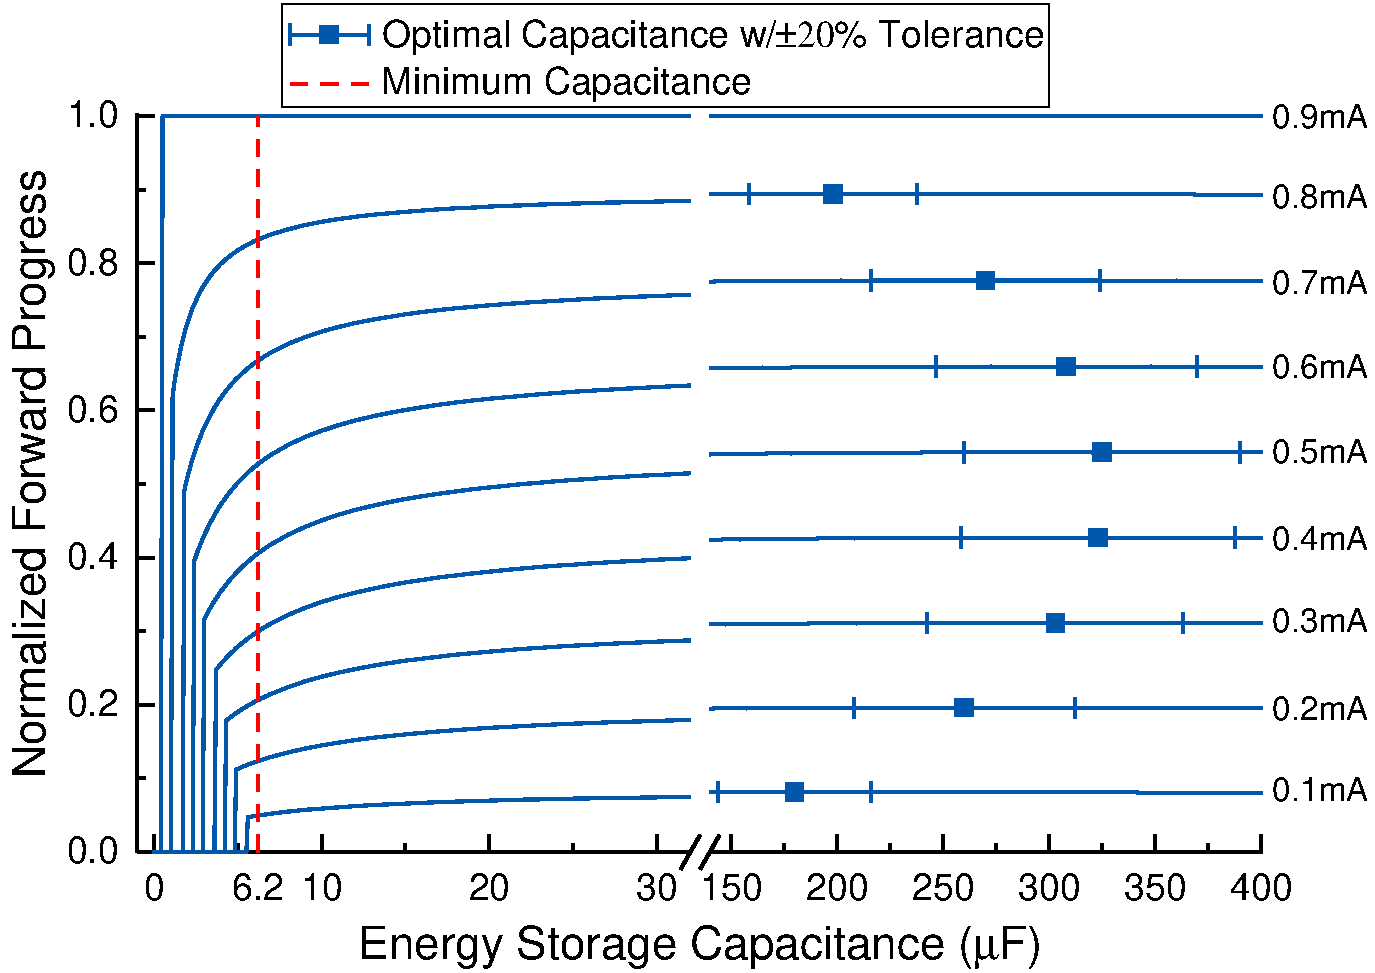
\includegraphics[width=3.2in]{ch3_sizingeffect/figures/StorCCur6Fig} 
  \caption{Forward progress against energy storage capacitance at different levels of constant supply current. Error bars around optimal points denote the impact of typical $\pm$20\% capacitance tolerance. }
  \label{fig:fpwconstcurr}
\end{figure}

\begin{figure}[!t]
  \centering
  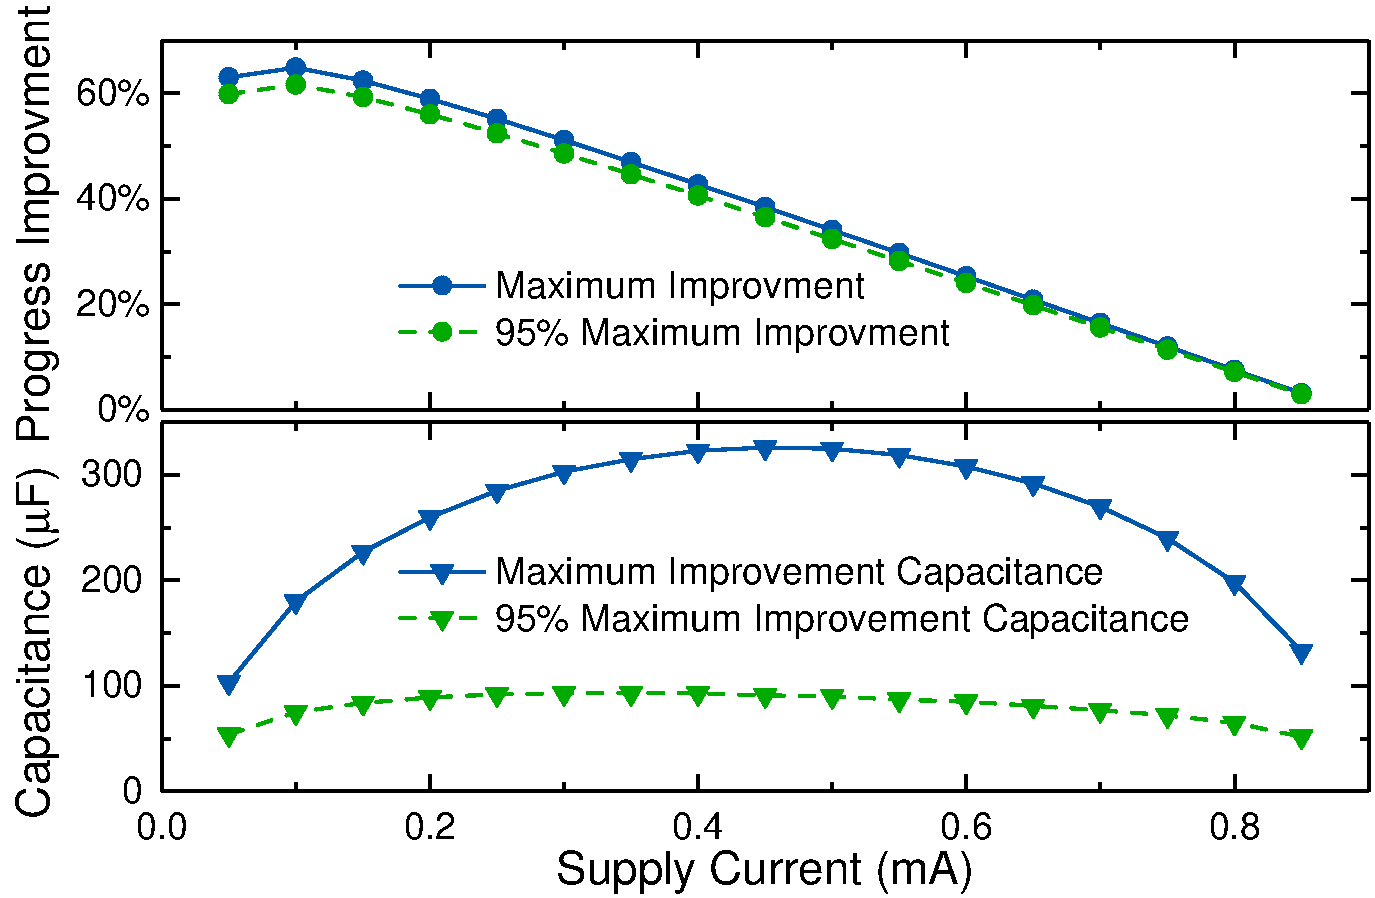
\includegraphics[width=3.2in]{ch3_sizingeffect/figures/StorCCurMax4Fig}
  \caption{Maximum forward progress improvement by sizing energy storage given a spectrum of supply current (normalized by the minimum capacitance case), with the corresponding maximum and sub-maximum (95\% of maximum) capacitance. }
  \label{fig:maxfwp}
\end{figure}

\figurename{~\ref{fig:maxfwp}} shows that an improvement in forward progress of up to 65\%  can be achieved when using the optimal capacitance instead of the minimum. However, it may not be desirable to set the capacitance solely for maximizing forward progress, because there are often trade-offs with other factors including increased interruption periods and dimensions. 
% (explored in Section~\ref{subsec:tradeoff}).
% In real-world energy source conditions, the supply current varies across this spectrum, and hence leads to an overall progress improvement based on its supply distribution. 
% This improvement exists only when the device operates in the Intermittent mode, since the device keeps either inactive in the Off mode or active in the On mode without the need for restoring and saving state. 
% Correspondingly, the optimal energy storage capacity is also plotted against supply current. 
% This optimal capacity exists because of the side effect of capacitor leakage; without capacitor leakage effect, the forward progress would keep approaching the ideal case (as explained in Section~\ref{subsec:formulation}). 
While a large improvement can be delivered with the optimal capacitance, as shown in \figurename{~\ref{fig:maxfwp}}, 95\% of this gain can still be obtained with significantly smaller capacitances (mean 31\% of the optimal value).
For example, reducing from \SI{325}{\micro\farad} to \SI{90}{\micro\farad} gives 95\% of the maximum improvement with a \SI{0.5}{\milli\ampere} supply. 

% in real deployment, storage fixed while current varies, change over a range, we may need to pick a capacity that optimise the majority of energy conditions. 

\subsubsection{Impact of Volatile State Size}

The size of volatile state differs across applications with different amounts of RAM usage, and hence incurs varying time and energy overheads for restore and save operations. We measured time overheads of restore and save operations in the minimum case (64B register data and a 160B stack) and the maximum case (64B register data and a full 2048B RAM) respectively as shown in Table~\ref{tab:ramscale}. As these time overheads are expected to be linear to the state size~\cite{Sliper:2019:ESR:3316781.3317812}, the model can be tuned for various volatile state sizes by linearly scaling the profiled values. 

% In the MCU we explore, volatile state includes CPU registers and SRAM data, which takes 64B and 160-2048B. 

\begin{table}[!t]
    \renewcommand{\arraystretch}{1.2}
    \centering
    \caption{Linear scaling range of volatile state size and restore/save time overheads}
    \label{tab:ramscale}
    \begin{tabular}{|c|cc|}
    \hline
    \textbf{State Size} & \multirow{2}{*}{\textbf{Restore Time}} & \multirow{2}{*}{\textbf{Save Time}}\\
    \textbf{(Registers + SRAM)} & & \\
    \hline
    64B + 160B (lower bound) & \SI{232}{\micro\second} & \SI{208}{\micro\second}\\
    % 64B registers + 160B stack
    64B + 2048B (upper bound) & \SI{2.298}{\milli\second} & \SI{2.274}{\milli\second} \\
    % 64B registers + 2048B RAM
    \hline
    \end{tabular}
\end{table}

An example of this is plotted in \figurename{~\ref{fig:ram}}. The forward progress improvement by sizing energy storage increases with the volatile state size, and the optimal capacitance grows accordingly. The improvement becomes insignificant when the volatile state size is small because the restore and save overheads are already negligible. For example, when the workload uses the least volatile state (the leftmost point), the maximum progress improvement is only 3.6\% although the restore and save overheads are reduced by 93\%. 
% This indicates the more efficiently ICSs save/restore, the more useless this work is. 

\begin{figure}[!t]
    \centering
    \includegraphics[width=3.2in]{ch3_sizingeffect/figures/RSTORAM3Fig}
    \caption{Impact of RAM usage (linear to restore/save overheads) on sizing energy storage with \SI{0.4}{\milli\ampere} current supply. Improvement and reduction are normalized by the minimum capacitance case. }
    \label{fig:ram}
\end{figure}
   
\section{Sizing under Real-World Energy Conditions} \label{sec:c4_demo}

In this section, we model an IPS with a PV energy harvester to explore the energy storage sizing effect in real-world energy conditions, and demonstrate use of the proposed sizing approach. 

\begin{figure}
    \centering
    \includegraphics[width=\columnwidth]{ch4_sizingapproach/figures/solarmodel4}
    \caption{System model of a PV-based IPS.}
    \label{fig:Model}
\end{figure}

\subsection{Simulation Configuration}

We integrate the validated reactive IPS model into a system model with a PV energy-harvesting supply as shown in \fref{fig:Model}. 
The energy storage model and the intermittent load model are as presented in \sref{sec:c3_exploration}. 

We use a converter-less supply circuit where only a Schottky diode is connected to the energy harvester output in order to prevent current backflow. 
The energy source conditions are imported from NREL outdoor solar irradiance data~\cite{stoffel1981nrel} and EnHANTs indoor irradiance data~\cite{6244798}. 
Four sets of light conditions are used to encompass different energy environments. 
To convert irradiance into harvested power, we adopt a PV cell model~\cite{en9050326} which uses the parameters available in common datasheets, so it can easily be reconfigured to suit various devices. 
The output current \nm{I}{o} of the PV cell model can then be described as:
\begin{equation} \label{eq:pvcell}
    \nmm{I}{o} = \frac{G}{\nmm{G}{ref}} \nmm{I}{sc} (1 - (1 - \frac{\nmm{I}{mpp}}{\nmm{I}{sc}}) ^ {\frac{\nmm{V}{o}-\nmm{V}{oc}}{\nmm{V}{mpp} - \nmm{V}{oc}}})
\end{equation}
where \nm{V}{o} is the output voltage of the PV cell, $G$ is the ambient irradiance, \nm{G}{ref} is the reference irradiance (normally \SI{1000}{\watt\per\square\centi\meter}), and \nm{I}{sc}, \nm{V}{oc}, \nm{I}{mpp}, \nm{V}{mpp} are respectively short-circuit current, open-circuit voltage, and the current and voltage at maximum power point (MPP) given the reference irradiance. 
\nm{V}{o} and $G$ are dynamic at run time, while other parameters in this model are constant. 
We refer to Panasonic Amorton glass type solar cells~\cite{solarcell} for PV cell properties as shown in \tref{tab:pvcell}. 
We set four cells in series (with \nm{V}{oc} = 3.56V) to match the operating voltage of the MCU (maximum 3.6V), and model energy harvester sizing by scaling the cell area. 


% A PV panel is an array of PV cells, which amplifies voltage and current output by connecting PV cells in series or parallel. In a PV panel, the open-circuit voltage is proportional to the number of cells in series, and the short-circuit current is proportional to the area of each cell and the number of cells in parallel. 

\begin{table}
    \renewcommand{\arraystretch}{1.2}
    \centering
    \begin{tabular}{|c|c|}
    \hline
    \textbf{Parameter} & \textbf{Value}\\
    \hline
    Open-Circuit Voltage & \SI{0.89}{\volt}/cell\\
    Short-Circuit Current & \SI{14.8}{\milli\ampere\per\square\centi\meter}\\
    Maximum Power Voltage & \SI{0.65}{\volt}/cell\\ 
    Maximum Power Current & \SI{12.1}{\milli\ampere\per\square\centi\meter}\\
    \hline
    \end{tabular}
    \caption{PV cell properties under a \SI{1000}{\watt\per\square\centi\meter}, AM-1.5 light source.}
    \label{tab:pvcell}
\end{table}

Our simulation tool can perform two simulation processes: (a) sort and process the time distribution of environmental conditions, and (b) simulate system state chronologically with a fine-grained time step. 
Process (a) reduces simulation time significantly, e.g. from hours to seconds, but ignores the restore operation after a brownout reset, hence overestimating forward progress, and it overestimates more with smaller capacitance and lower supply current. 
In the following results, \fref{fig:harvstor} comes from Process (a) for fast exploration, and \fref{fig:interruption} and \fref{fig:tradeoff} come from Process (b) for accurate records of interruption periods. 

\subsection{Exploration with Real-World Energy Source Conditions} \label{subsec:harvstor}

% Goal: 
% 1. to show that this model can help designers to find a suitable size of EH to achieve their desired performance;
% 2. to show that sizing energy storage would have different degrees of impact on real deployment depending on the specific energy conditions;
% 3. demonstrate sizing approach. 

In real-world deployments, ambient energy source conditions are dependent on time and location. 
The energy harvester and storage need to be sized to achieve the desired forward progress across the range of expected conditions. 

\subsubsection{Sizing the Energy Harvester}

For the purposes of this exploration, three levels of baseline mean forward progress (\nm{\alpha}{exe}) are set as 0.1, 0.2, and 0.3. 
We use the system model to find the PV panel area that achieves the expected forward progress under the different energy source conditions with minimum energy storage. 
We scale the PV panel area to find that which achieves each baseline \nm{\alpha}{exe}. 
As shown in \fref{fig:harvstor}, the energy harvester sizes that achieve the desired \nm{\alpha}{exe} may span orders of magnitude given different energy source conditions from \SI{}{\square\milli\meter} for outdoor sources ((c) and (d)) to \SI{}{\square\centi\meter} for indoor sources ((a) and (b)).  

\subsubsection{Sizing the Energy Storage}

Having obtained the energy harvester sizes for the baseline forward progress, we then use the modelling approach to size energy storage.
% A table lists the PV panel area to achieve the target \nm{\alpha}{exe} with minimum energy storage capacitance, the optimal capacitance with the forward progress improvement, and the alternative (decreased) PV panel area with the optimal capacitance. 
We analyse the sizing effect of energy storage on forward progress given real-world energy conditions. \fref{fig:harvstor} shows a 7.8-43.3\% improvement in forward progress by sizing energy storage under the given real-world energy conditions and baseline energy harvester sizes. 
It can also be inferred that optimising energy storage can either improve forward progress for a given energy harvester size, or reduce the energy harvester size that achieves the target forward progress. 
Given higher-power energy sources (e.g. Denver 2018 and Hawaii 2018 outdoor solar), increasing the harvester size efficiently improves forward progress with minor dimensional overheads, e.g. tens of \SI{}{\square\milli\meter}; however, given lower-power sources (e.g. EnHANTs Setup~A and Setup~D indoor light), optimising energy storage capacitance can save tens of \SI{}{\square\centi\meter} of PV panel area to achieve the same forward progress.

Also, the progress improvement by sizing energy storage varies accordingly with energy source conditions. 
As mentioned in \cref{chapter:sizingeffect}, this improvement stems from the reduction of restore and save overheads when the supply current is low and the device work in the \textit{Intermittent} mode. 
Thus, the results of EnHANTs Setup~A and Setup~D show a higher progress improvement from sizing energy storage than those of Denver 2018 and Hawaii 2018. 

\begin{figure}
    \centering
    \begin{subfigure}{0.51\columnwidth}
        \centering
        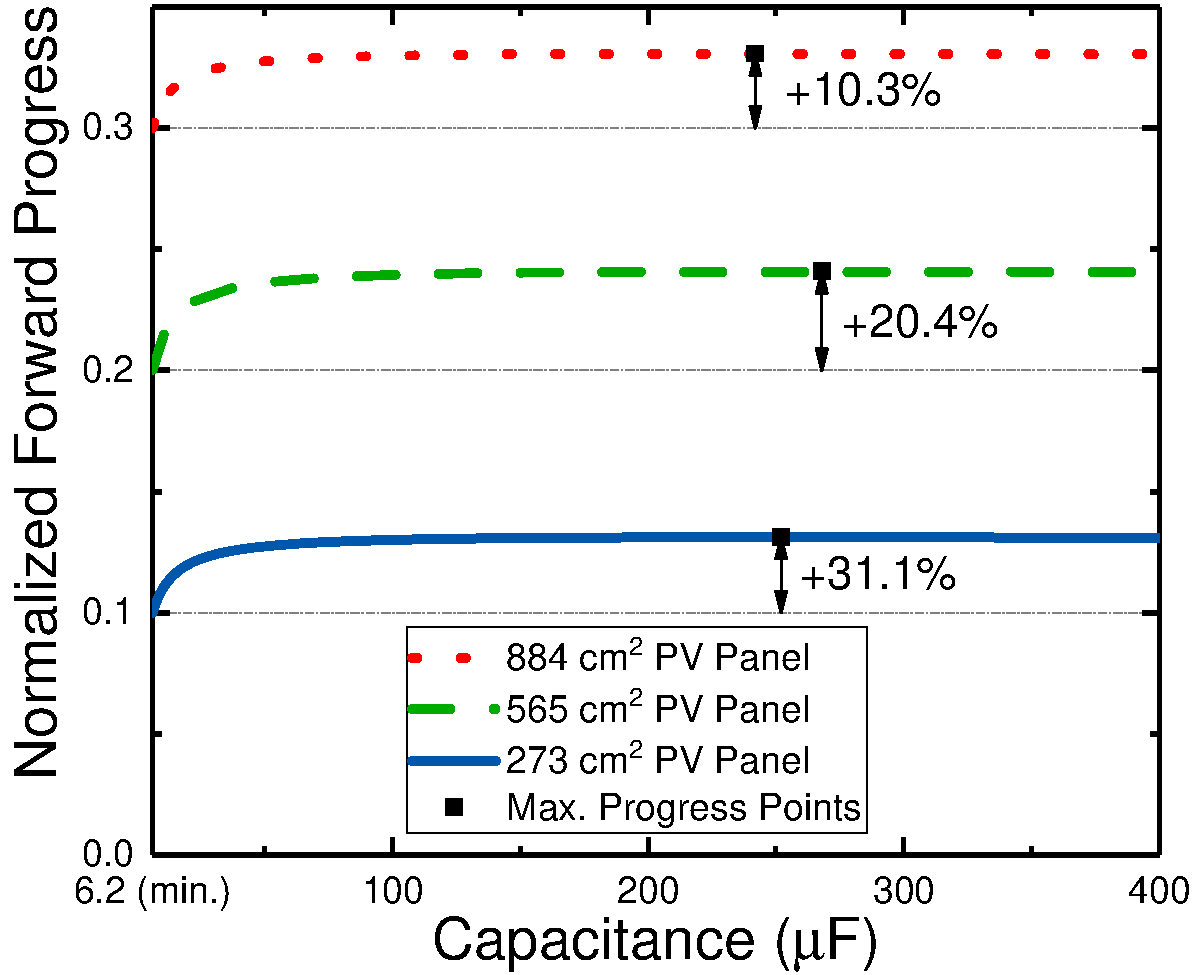
\includegraphics[width=\columnwidth]{ch4_sizingapproach/figures/HarvStorTgFig1}
        \caption{EnHANTs Setup A}
        \label{fig:harvstor1}
    \end{subfigure}
    \begin{subfigure}{0.483\columnwidth}
        \centering
        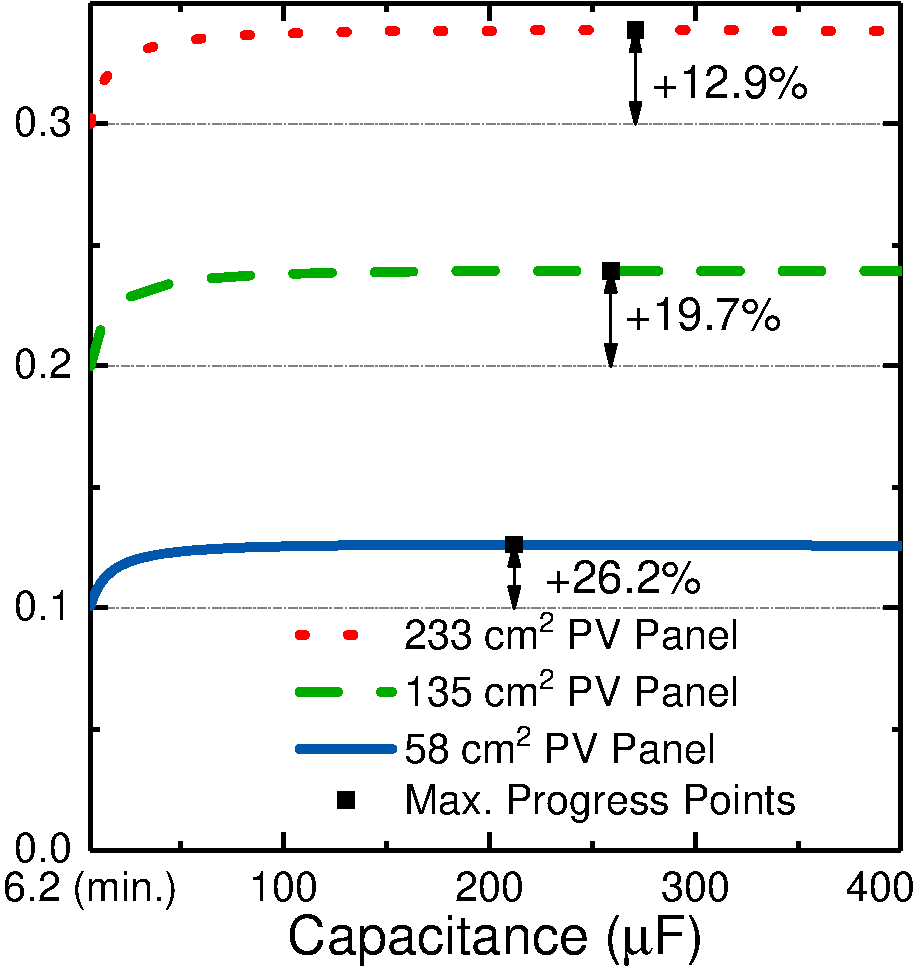
\includegraphics[width=\columnwidth]{ch4_sizingapproach/figures/HarvStorTgFig2}
        \caption{EnHANTs Setup D}
        \label{fig:harvstor2}
    \end{subfigure}
    \hfil
    \begin{subfigure}{0.51\columnwidth}
        \centering
        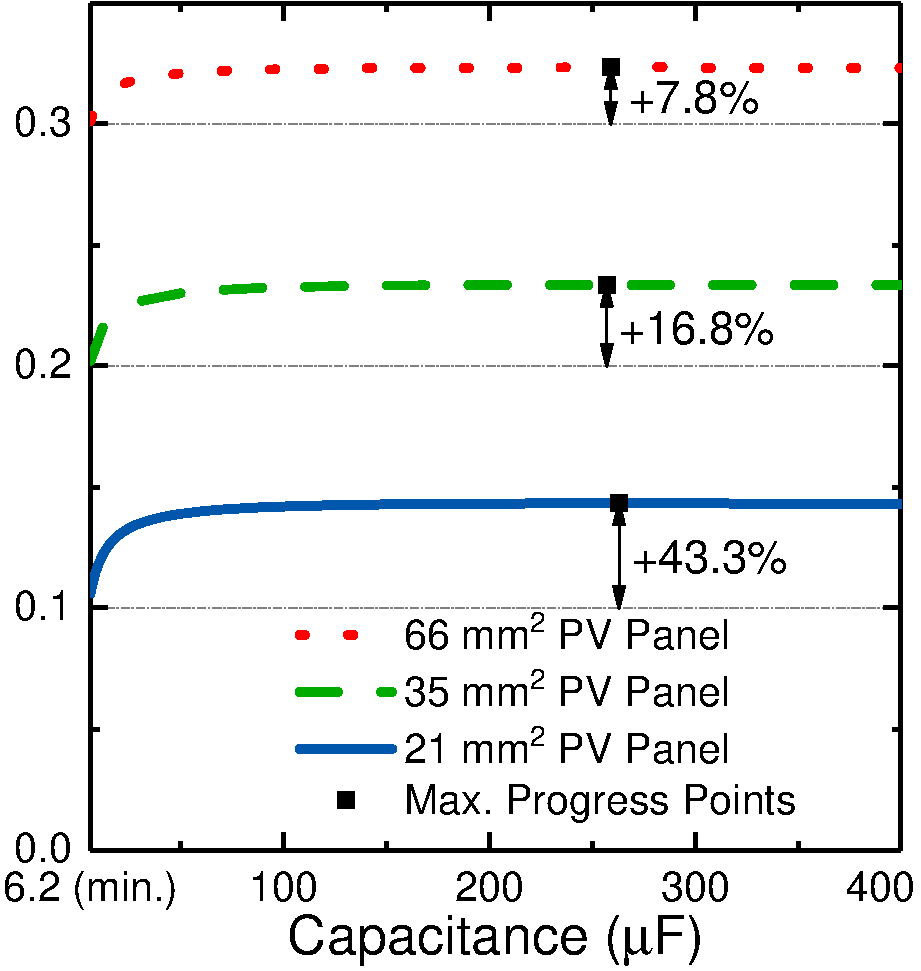
\includegraphics[width=\columnwidth]{ch4_sizingapproach/figures/HarvStorTgFig3}
        \caption{NREL Denver 2018}
        \label{fig:harvstor3}
    \end{subfigure}
    \begin{subfigure}{0.483\columnwidth}
        \centering
        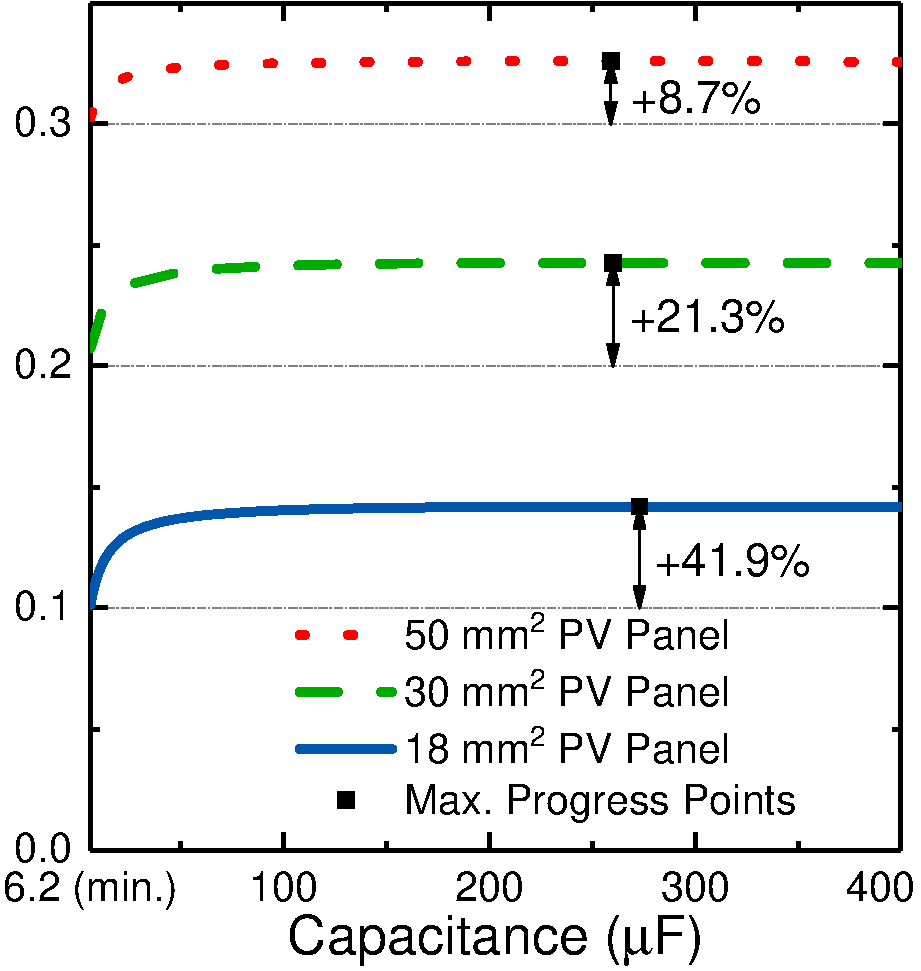
\includegraphics[width=\columnwidth]{ch4_sizingapproach/figures/HarvStorTgFig4}
        \caption{NREL Hawaii 2018}
        \label{fig:harvstor4}
    \end{subfigure}
    \caption{Improvement of average forward progress by sizing energy storage given different PV panel areas under real-world energy source conditions. The model is able to find the PV panel area required for achieving the target mean forward progress. } 
    \label{fig:harvstor}
\end{figure}

The mean forward progress given target \nm{\alpha}{exe} = 0.1 is plotted in \fref{fig:harvstorrange}, with the 60th and 90th time percentiles of forward progress. In all the  above datasets, the energy source is absent and the system is off for around \SI{55}{\percent} of time, so we plot the percentiles from the 60th. The mean progress during the energy-available periods is averaged over the energy-absent periods, so the actual mean forward progress during the energy-available periods is nearly double the annual mean. 

% Absolute improvement are different? Large variations? What other results can I add? 
% The variations of forward progress are significant due to the large variations of energy source conditions, so practical implementation should consider such variation as .
% The improved progress during the energy-available periods is averaged over the energy-absent periods, so the actual amount of improvement when energy is available is higher than the mean. (wrong statement)

\begin{figure}
    \centering
    \begin{subfigure}{0.51\columnwidth}
        \centering
        \includegraphics[width=\columnwidth]{ch4_sizingapproach/figures/HarvStorRan2Fig1}
        \caption{EnHANTs Setup A}
        \label{fig:harvstorrange1}
    \end{subfigure}
    \begin{subfigure}{0.483\columnwidth}
        \centering
        \includegraphics[width=\columnwidth]{ch4_sizingapproach/figures/HarvStorRan2Fig2}
        \caption{EnHANTs Setup D}
        \label{fig:harvstorrange2}
    \end{subfigure}
    \hfil
    \begin{subfigure}{0.51\columnwidth}
        \centering
        \includegraphics[width=\columnwidth]{ch4_sizingapproach/figures/HarvStorRan2Fig3}
        \caption{NREL Denver 2018}
        \label{fig:harvstorrange3}
    \end{subfigure}
    \begin{subfigure}{0.483\columnwidth}
        \centering
        \includegraphics[width=\columnwidth]{ch4_sizingapproach/figures/HarvStorRan2Fig4}
        \caption{NREL Hawaii 2018}
        \label{fig:harvstorrange4}
    \end{subfigure}
    \caption{Time percentiles of forward progress by sizing energy storage with target \nm{\alpha}{exe} = 0.1 and the corresponding PV panel area listed in \fref{fig:harvstor}. The percentiles start from the 60th as the system is off for around \SI{55}{\percent} of time due to insufficient energy source. }
    \label{fig:harvstorrange}
\end{figure}

\subsubsection{Interruption Period} \label{subsubsec:intper}
Besides forward progress, we also explore how the capacitance can change the interruption periods. 
When interrupted by insufficient power supply, an IPS enters an interruption period where it saves its volatile state, waits for supply voltage to recover, and restores the state to resume execution, without making any forward progress. 
Applications that require frequent sensing may be negatively affected by long interruption periods. 
We measure an interruption period as \textit{the period between two successive execution periods}, e.g. a consecutive `SLR' period in \fref{fig:operatingCycle} forms an interruption period. 
We record all the interruption periods during a one-year simulation with \SIrange{10}{50}{\micro\farad} capacitors, the Denver 2018 dataset, and an \SI{80}{\square\milli\meter} PV panel. 
\fref{fig:interruption} presents the distribution of all the interruption periods. 
With increased energy storage, the interruption period is prolonged. 
For example, the 90th percentile of interruption periods increases from \SI{32.2}{\milli\second} at \SI{10}{\micro\farad} to \SI{123.4}{\milli\second} at \SI{50}{\micro\farad} at an approximate rate of \SI{23}{\milli\second} per \SI{10}{\micro\farad}. 
% The majority of the interruption periods are within \SI{200}{\milli\second}. 
Facilitated by the simulator, developers are enabled to estimate whether the distribution of interruption periods meet their application requirement. 

% Whether and how much this would affect  Time-sensitive applications may care 
% the total number of interruptions is reduced,


\begin{figure}
    \centering
    \includegraphics[width=\columnwidth]{ch4_sizingapproach/figures/IntPeriodOrdFig}
    \caption{Distribution of interruption periods. }
    \label{fig:interruption}
\end{figure}

\subsection{Trading Forward Progress, Dimensions, and Interruption Period} \label{subsec:tradeoff}

Although increasing energy storage capacitance improves forward progress, larger capacitance increases both dimensions and interruption periods. 
We evaluate the overheads of increased capacitor dimensions and interruption periods, and then trade them off against forward progress using a cost function to suggest an optimal capacitance value. 

\subsubsection{Metric of Dimensions}

The overhead of capacitor dimensions is evaluated by characteristics of off-the-shelf tantalum capacitors. 
We narrow down the range of sample capacitors within a set of characteristics: low-profile, 10V rated voltage, and surface-mount package, and select six series of capacitors\footnote{The series of capacitor considered were: AVX TAJ, AVX TACmicrochip, AVX F92, Vishay 572D, Vishay 591D, and Vishay 592D.}. 
The volume and capacitance of these devices are plotted in \fref{fig:capvol}. 
We use the regression of these data to approximate a capacitance-volume relationship.
% ~\cite{tancap1, tancap2, tancap3, tancap4, tancap5, tancap6}
% Among the common capacitor chemistries with \textmu F to mF capacitance, tantalum capacitors manifest low leakage 

\begin{figure}
    \centering
    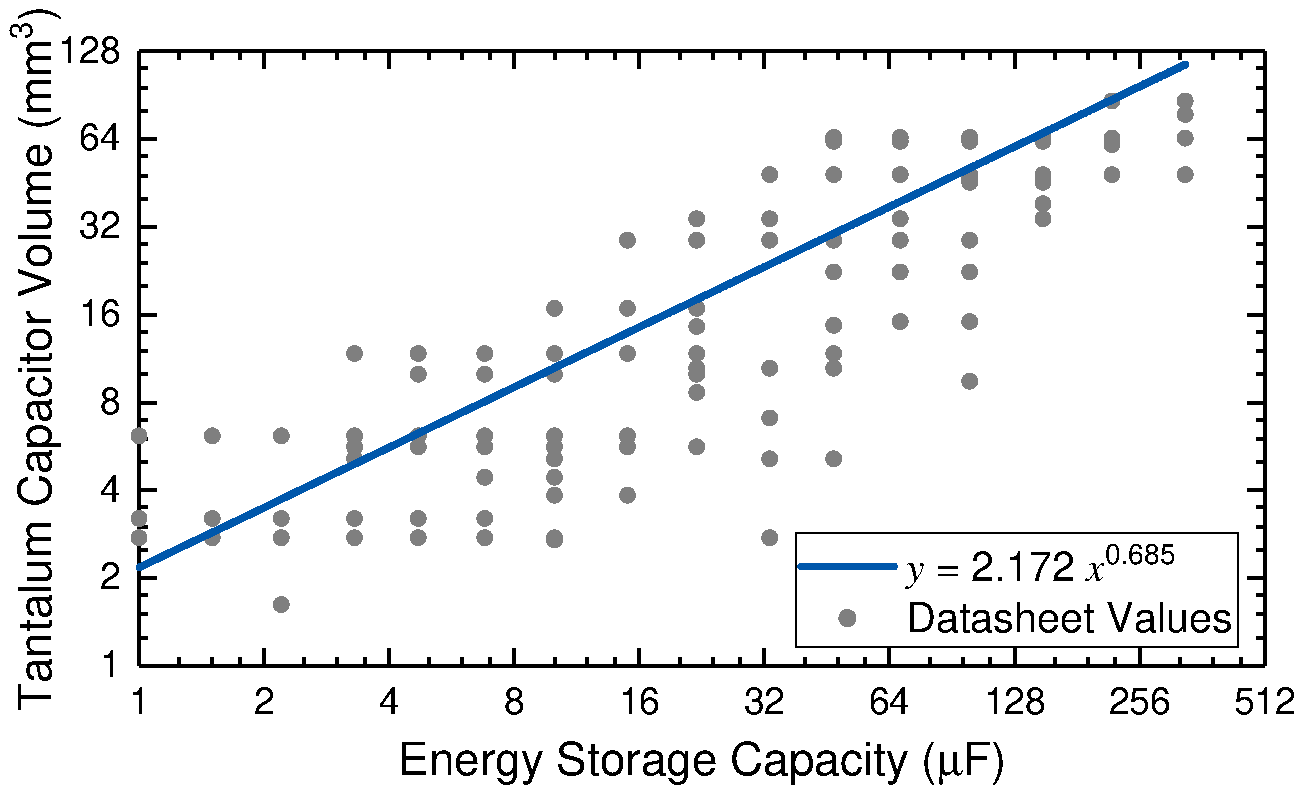
\includegraphics[width=\columnwidth]{ch4_sizingapproach/figures/CapVol2Fig2}
    \caption{Tantalum capacitor volume against capacitance for the six series of capacitors analysed. }
    \label{fig:capvol}
\end{figure}

\subsubsection{Metric of Interruption Periods} \label{subsubsec:metricintper}

% Definition/Measurement of interruption periods. recharging ability? Considering leakage?
% why interruption periods is important, why we consider it.

% , i.e. the period that does not make forward progress. The total interruption periods should be opposite to forward progress. 
Applications may have various requirements on interruption periods. 
To demonstrate the usage of our sizing approach, we consider a designer requests the 90th percentile of all interruption periods as an example metric of interruption periods, denoted as \nm{T}{int}. 
This metric indicates 90\% of interruption periods are shorter than \nm{T}{int}. 
This metric can be adapted for particular application requirements. 
% In We assume that $T_{interrupt}$ is preferable to be short for general application. 

\subsubsection{Cost Function}

From the previous observations (\fref{fig:maxfwp}) we can see that achieving the optimal progress improvement costs much more capacitance (mean 3.2$\times$) than to achieve 95\% improvement. 
A trade-off is necessary to improve forward progress while restricting the overheads of increased capacitor volume and interruption periods. 
This involves a problem of multi-criteria decision making~\cite{triantaphyllou2000multi}, which is outside the scope of this work. 
Nevertheless, we provide a cost function in (\ref{eq:tradeoff}) as an example to illustrate how these three factors could be traded-off, but designers are expected to customise a cost function with parameters of importance to specific application requirements. 
Note that the function (\ref{eq:tradeoff}) is to be maximised to find the recommended capacitance. 
\begin{equation}
    f = \frac{\nmm{\alpha}{exe}}{\nmm{k}{1}} - \left(\frac{\nmm{v}{cap}}{\nmm{k}{2}}\right) ^ {2} - \left(\frac{\nmm{T}{int}}{\nmm{k}{3}}\right) ^ {2} 
    \label{eq:tradeoff}
\end{equation}
\nm{\alpha}{exe} denotes normalised forward progress, \nm{v}{cap} denotes capacitor volume, and \nm{T}{int} denotes application interruption periods as mentioned in \sref{subsubsec:metricintper}. 
\nm{\alpha}{exe}, \nm{v}{cap}, and \nm{T}{int} can be generated from the simulation tool given $C$ as an input. 
\nm{k}{1}, \nm{k}{2}, and \nm{k}{3} are coefficients for normalising each metric, and they are empirically determined according to applications. 
In this example, the undesirable parameters are expressed as quadratic and negative terms to give an increasing cost to higher values. 
While only three parameters are considered here, others (such as the energy harvester size) could be included for a system-wise sizing scenario.
As an example to demonstrate its usage, we arbitrarily configure the function by setting \nm{k}{1} = 0.2, \nm{k}{2} = \SI{200}{\cubic\milli\meter}, and \nm{k}{3} = \SI{500}{\milli\second}. 
%, i.e.:
%\begin{equation}
%    f = \frac{\nmm{\alpha}{exe}}{0.2} - (\frac{\nmm{v}{cap}}{200}) ^ {2} - T_{recharge} ^ {2} 
%    \label{eq:tradeoffuse}
%\end{equation}
% where \nm{v}{cap} is in \SI{}{\cubic\milli\meter} and $T_{recharge}$ is in second. Here, $\frac{1}{\nmm{k}{1}} / \frac{1}{\nmm{k}{2}}$ equals 1000, but this does not mean that forward progress is 1000 times more important than capacitor volume.

\subsubsection{Results}

The effect of the trade-off is plotted in \fref{fig:tradeoff} using the Denver 2018 energy source dataset. 
Compared to the capacitor size that solely maximises forward progress, on average, an appropriately-sized capacitor achieves 93\% of the maximum forward progress, while saving 83\% of capacitor volume and 91\% of interruption periods. 
This also demonstrates the efficacy of the cost function and the chosen coefficients. 
Compared to the minimum storage case, the appropriately-sized capacitor improves forward progress by 12-124\% with energy storage increased from \SI{6.2}{\micro\farad} to \SI{30}{\micro\farad}.

\begin{figure}
    \centering
    \includegraphics[width=\columnwidth]{ch4_sizingapproach/figures/Tradeoff3Fig}
    \caption{The sizing approach trades off forward progress, capacitor volume, and interruption periods. The results are plotted against a range of PV panel area, given Denver 2018 energy source dataset. }
    \label{fig:tradeoff}
\end{figure}

As shown in \fref{fig:capvol}, the closest available capacitance that satisfies the \SI{6.2}{\micro\farad} minimum capacitance is \SI{6.8}{\micro\farad}, whereas the closest available capacitance to the appropriate \SI{30}{\micro\farad} is \SI{33}{\micro\farad}. 
The minimum volumes of \SI{6.8}{\micro\farad} and \SI{33}{\micro\farad} capacitors are both \SI{2.75}{\cubic\milli\meter}, which means using the appropriate capacitance, instead of the minimum one, may not incur dimensional overhead. 
% For \SI{47}{\micro\farad}, the absolute volume (\SI{5.12}{\cubic\milli\meter}) is insignificant compared to the device as a whole, e.g. an MSP430FR6989 MCU chip alone occupies \SI{274.4}{\cubic\milli\meter} (14 $\times$ 14 $\times$ 1.4). 
The regressed volume of the above two capacitance values are \SI{8.1}{\cubic\milli\meter} and \SI{23.8}{\cubic\milli\meter} respectively. 
However, the selection of capacitors can be dependent on factors other than physical volume, such as reliability, operation temperature, and more specific application needs. 
These factors can also be added into the cost function if necessary. 
% Again, such a volume scale is still insignificant in a whole device. 

            


\section{Conclusions} \label{section:conclusion}

% We explored the relationship between forward progress and energy storage capacitance in intermittent computing through a theoretical model.

% In this paper, we presented a model of reactive ICSs that accurately estimates forward progress. 
% Using this model, we explored the sizing effect of energy storage on forward progress with respect to supply current and volatile state size, showing up to \SI{64.9}{\percent} progress improvement under constant current supply and \SIrange{7.8}{43.3}{\percent} improvement on annual mean forward progress 
% under various real-world energy conditions. 

While conventional ICSs have used minimal levels of capacitance, this paper has shown that increasing the amount of energy storage can improve system performance by up to 65\% with a constant current supply and 43\% with real-world PV sources. The work includes a simulation tool which is available to download, enabling researchers to experiment with energy storage sizes to optimize ICS designs. A cost function can be incorporated, allowing various aspects of system performance to be traded-off. Our conclusion is that energy storage should be carefully designed, rather than minimized or indiscriminately picked, to efficiently operate ICSs.
% %% ----------------------------------------------------------------
%% Currentwork.tex
%% ---------------------------------------------------------------- 
\chapter{Effect of Energy Storage Capacity on Power-Neutral Computing} \label{Chapter:Work2}

% Old: This chapter presents a preliminary work on evaluating the effect of energy storage size on forward progress when given an increased capacity (compared to PN systems) of the energy storage under a control scheme adopted in prior PN systems. The varying harvested energy is balanced within seconds due to the increased storage capacity, which leads to a more flexible control of performance scaling. 

% Poster Abstract: Energy harvesting sources have inherited temporal and spatial variability, which is previously overcome by large energy buffers in the form of batteries. Power neutral computing is proposed to tackle the problems involved in battery usage, whereby the instantaneous power consumption is matched with the instantaneous harvested power through dynamic performance scaling with a minimum storage. However, a PN system has to scale its performance and power consumption quickly and passively, rather than actively select the operating points, which might not be ideal in terms of forward progress. This poster evaluates the forward progress when given an increased capacity of the energy storage under a control scheme adopted in prior power neutral systems. Simulation results show that the forward progress can be improved by up to 12% when properly designing an energy storage.

Energy-neutral computing is an established paradigm, which balances the harvested energy against the energy consumption over a period of time by incorporating sufficient energy storage. Unfortunately, large energy storage increases the volume and cost of devices. Recently, power-neutral computing has been proposed to exploit harvested power using only negligible energy storage by matching the instantaneous power consumption with the instantaneous harvested power. However, due to over-reduction of energy storage, significant performance variations in power-neutral computing may cause performance loss. This chapter presents how an increased amount of energy storage affects the overall system performance, i.e. application throughput. The optimal amount of energy storage is explored, providing a design consideration for selecting the right amount of energy storage in an energy harvesting computing system. As evaluated in simulation based on empirical data of a system-on-chip platform, given a time-varying harvested power trace, properly sizing the energy storage delivers a 14.6\% performance improvement, compared to a state-of-the-art power-neutral system, while maintaining the performance scaling scheme. 

\section{Overview}

% The advent of energy harvesters enables a transformation in the powering method of wireless devices from tethered or battery power into harvested power~\cite{beeby2010energy}. Energy harvesting is to generate electricity from scavenging ambient energy sources, such as light, wind, heat, electromagnetic waves, etc. Energy harvesters can significantly prolong the lifetime of wireless sensor nodes~\cite{jayakumar2016energy}. However, energy harvesting sources have inherent temporal and spatial variability, which contradicts a basic requirement of conventional electronic devices: a stable power supply~\cite{sudevalayam2011energy}. 

% In order to cope with this challenge, 
EN computing separates the load from the energy harvesting power supply with large energy storage, which smooths out differences between the harvested energy and the consumed energy over a long period, such as a few hours~\cite{kansal2007power}, a few days~\cite{sharma2010cloudy}, one year~\cite{buchli2014dynamic}, etc. EN systems maintain a service level over a required period of time so that the total energy consumption equals the total harvested energy~\cite{kansal2007power}. Large energy buffers in EN computing work well in compensating and balancing energy variation, which ensures task execution whether the harvested power is available or not. However, the widespread use of batteries and supercapacitors poses environmental and maintenance issues~\cite{peng2012throughput, raghunathan2005design}, and increases the volume of devices, which contradicts the design requirements in some cases, e.g. wearable devices~\cite{mitcheson2010energy, acampora2013survey}.

Without adding large energy storage as EN computing does, PN computing efficiently utilises harvested energy by matching the instantaneous power consumption with the instantaneous harvested power. However, strict power tracking in PN systems leads to significant performance variations due to the fluctuation of the harvested power. Such variations may reduce the overall performance (the total amount of completed execution divided by execution time) because of a convex relationship between the system power consumption and the clock frequency in DVFS.

Allocating more energy storage than the minimum level can mitigate this performance variation by constraining the variation of the supply voltage, and hence improve the overall performance. However, increasing energy storage also impedes the performance growth after systems are woken up and respond to a power pulse in a limited time. Also, the energy stored in the capacitor below the minimum operating voltage of the system is effectively wasted, and it takes more time to charge up larger capacitors. Therefore, there is a trade-off between the pros and cons of having a certain amount of energy storage with respect to the system overall performance. 

This chapter presents a methodology to improve system performance by selecting an optimal amount of energy storage given time-varying harvested power. The contributions of this work includes
\begin{itemize}
    \item A theoretical analysis of why adding a certain amount of energy storage to the minimum level improves the overall performance in an energy harvesting system adopting DVFS for performance scaling. 
    \item A model of an energy harvesting computing system using experimental data of a SoC platform, and simulations that evaluate the optimal amount of energy storage and explain the system behaviours.
\end{itemize} 

\section{Problem Identification}

Dynamic performance variations are a typical characteristic of PN computing. This section illustrates the reason why reducing the performance variations improves the overall performance in DVFS-based PN computing, and then, why increasing the minimised energy storage in PN computing supports such improvement.

\subsection{Performance Improvement in DVFS}

Theoretically, CPU power dissipation can be expressed as:
\begin{equation} \label{eq:cpupower}
    P_{CPU} = a V + b f + c f V^2
\end{equation}
where $a,b,c$ are constant parameters determined by hardware when the workload is constant, $V$ is the core voltage, and $f$ is the operating frequency of CPU~\cite{travers2015cpu}. When $f$ changes, the minimum voltage requirement for supporting this frequency changes accordingly. Assume that in DVFS settings, $V$ is adjusted to the minimum required level for every $f$, and hence $P_{CPU}$ is reduced to the minimum level. According to Equation~\ref{eq:cpupower}, $P_{CPU}$ is a quadratic function of $f$, and hence this function $P_{CPU}(f)$ is convex, nondecreasing and nonnegative. 
%When the system can execute tasks at different speeds by scaling performance using DVFS, the CPU power consumption is a convex function of the clock frequency (computing speed)~\cite{irani2007algorithms}.

Here, we denote $P(\alpha)$ as the total power consumption of a system when executing applications at speed $\alpha$ (a performance metric according to specific applications, typically linear to the operating frequency). When the system performs a CPU intensive application, $P_{CPU}$ constitutes the majority of $P(\alpha)$ and $P(\alpha)$ is a convex, nondecreasing and nonnegative function of $\alpha$.
%here, 'CPU intensive' is mentioned. But how to make sure that CPU consumption is still a large part when the load is performing other types of workloads, e.g. sensing tasks? Is it rigorous here?

Based on the convexity of $P(\alpha)$, we examine a case when the system is active and uninterruptedly executes tasks over a certain duration, and the performance scaling method of this system is DVFS. The convexity of $P(\alpha)$ leads to a phenomenon that, when consuming the same amount of energy within the same length of time, maintaining a constant speed renders higher overall performance than switching between two speeds. The proof and explanation of this are shown below. 

Assume that there are three points on $P(\alpha)$ at speed $\alpha_1,\alpha_2,\alpha_3$ and $0 < \alpha_1 < \alpha_2 < \alpha_3$, and hence $0 < P(\alpha_1) < P(\alpha_2) < P(\alpha_3)$. When the energy cost of maintaining speed $\alpha_2$ equals the energy cost of switching between $\alpha_1$ and $\alpha_3$ within a time duration $T$, the following equation is met:
\begin{equation} \label{eq:dvfs1}
    P(\alpha_2)T = P(\alpha_1)t + P(\alpha_3)(T-t)
\end{equation}
where $t$ is the time spent in operating at $\alpha_1$. Hence, $t$ can be calculated from Equation~\ref{eq:dvfs1} as:
\begin{equation} \label{eq:dvfs2}
    t = \frac{P(\alpha_3)-P(\alpha_2)}{P(\alpha_3)-P(\alpha_1)} T
\end{equation}
Due to the convexity of $P(\alpha)$, the following expression is met:
\begin{equation} \label{eq:dvfs3}
    \frac{P(\alpha_3)-P(\alpha_2)}{\alpha_3-\alpha_2} > \frac{P(\alpha_3)-P(\alpha_1)}{\alpha_3-\alpha_1}
\end{equation}
and this can be transformed to:
\begin{equation} \label{eq:dvfs4}
    (\alpha_3 - \alpha_1) \frac{P(\alpha_3) - P(\alpha_2)}{P(\alpha_3) - P(\alpha_1)} T - (\alpha_3 - \alpha_2) T > 0
\end{equation}
By substituting Equation~\ref{eq:dvfs3} into Equation~\ref{eq:dvfs4}, we can get:
\begin{equation} \label{eq:dvfs5}
    \alpha_2 T > \alpha_1 t + \alpha_3 (T - t)
\end{equation}

In Equation~\ref{eq:dvfs5}, the left is the computation done by operating at $\alpha_2$ throughout duration $T$ and the right is the computation done by switching between $\alpha_1$ and $\alpha_3$. Equation~\ref{eq:dvfs2} is true, so Equation~\ref{eq:dvfs5} is true. Therefore, operating at $\alpha_2$ outperforms switching between $\alpha_1$ and $\alpha_3$. The improvement on the overall performance $\eta$ in percentage is: 
\begin{equation} \label{eq:dvfs6}
    \eta = \frac{\alpha_2 T - [\alpha_1 t + \alpha_3 (T - t)]}{\alpha_1 t + \alpha_3 (T - t)} \times 100\%
\end{equation}
By substituting Equation~\ref{eq:dvfs3} into Equation~\ref{eq:dvfs6}, this improvement can be expressed as:
\begin{equation} \label{eq:dvfs7}
    \eta = \frac{\alpha_2 [P(\alpha_3) - P(\alpha_1)]}{\alpha_1 [P(\alpha_3) - P(\alpha_2)] + \alpha_3 [P(\alpha_2) - P(\alpha_1)]} \times 100\%
\end{equation}

Based on Equation~\ref{eq:dvfs5} which examines a case of three points, we conclude that oscillating between two frequencies renders less overall performance than maintaining one frequency between them when consuming the same amount of energy in the same time length. We can expand this conclusion to a case of four points, where oscillating between the two outer frequencies delivers lower overall performance than oscillating between two closer frequencies in the middle of them. Likewise, we can further obtain a case applied for several performance points: reducing the varying range of performance in DVFS results in higher overall performance when systems consume the same amount of energy in the same period. Besides, if $\alpha_1$ and $\alpha_3$ in Equation~\ref{eq:dvfs7} represent the highest and lowest computing frequencies of the scaling range, Equation~\ref{eq:dvfs7} represents the upper bound of improvement in the overall performance.

\subsection{Function of Energy Storage}

Based on the aforementioned analysis, this part illustrates how increasing the amount of energy storage above the minimum delivers performance improvement in systems incorporating DVFS.

\begin{figure}[!tb]
    \centering
    \includegraphics[width=12cm]{figure/work2/pnanalysis}
    \caption{Example of (a) a time-varying harvested power trace and (b) a system's convex power function.}
    \label{Figure:pnanalysis}
\end{figure} 

As illustrated in~\fref{Figure:pnanalysis}, the left is a trace of time-varying harvested power, and the right is a convex power function of a system. $P_{average}$ is the average harvested power during this time duration. $\alpha_2$ and $\alpha_3$ are the closest two operating points to $P_{average}$ on the power function, delivering the best average performance (in practice, the power function is discrete and there is probably not an operating point that exactly consumes $P_{average}$).

In prior PN works~\cite{balsamo2016graceful, fletcher2017power}, when given only minimum storage for the system to switch the operating point, the proposed solution is to match the power consumption with the input power trace as closely as possible, such that the system utilises the harvested power to the maximum. Specifically, if the small amount of storage can hardly tolerate any power difference, the power consumption can only go just beyond or just below the instantaneous input power anytime. Otherwise, the system stops or the harvested power is wasted. To achieve power matching, the system has to frequently and widely switch among several points between $\alpha_1$ and $\alpha_4$ when responding to the given power trace in~\fref{Figure:pnanalysis}(b).

When the storage is increased from this minimum amount, the system is able to tolerate more temporary power variation. If the storage is large enough to balance the energy over this whole duration, according to the prior analysis, in order to output the highest overall performance within this time duration, the best solution in practice is to oscillate between $\alpha_2$ and $\alpha_3$ for the whole period, rather than scale the frequency across a wider range between $\alpha_1$ and $\alpha_4$. This is why an increased amount of energy storage can improve the overall performance: enabling more energy inequality and allowing more freedom in selecting the operating point and processing tasks. 

However, larger energy storage also introduces longer latency in responding to a power pulse, which leads to inefficient use of harvested energy in both "cold starts" and performance adaptation. Therefore, there is a trade-off between having an amount of energy storage to offset significant power changes and the latency it brings. This trade-off is further evaluated in this work.

\section{System Modelling}

A model is built to evaluate the effect of the amount of energy storage on the overall performance of an energy harvesting computing system. The model structure is based on a simplified architecture of a PN system as shown in~\fref{Figure:modelarch}. This system consists of three main components: an energy harvester, energy storage (a capacitor), and a computing load. These three components are linked by power flows indicated as $P_h$ and $P_c$ representing the harvested power and the system power consumption respectively. Also, the energy harvester is decoupled from the remaining part by a diode to prevent the power backflow, so $P_h \geq 0$ is ensured.

\begin{figure} [!tb]
    \centering
    \includegraphics[width=10cm]{figure/work2/modelarch}
    \caption{Simplified architecture of a PN system.}
    \label{Figure:modelarch}
\end{figure} 

\subsection{Energy Harvester}

The energy harvester is modelled by a time-varying power trace, i.e. harvested power against time. This trace can be either taken from the output data of real energy harvesters, or an arbitrary power trace, such that the simulation based on this model can include different power conditions with flexibility. 

\subsection{Energy Storage}

The energy storage is modelled as an ideal capacitor with the following assumptions: a) no leakage; b) 100\% changing and discharging efficiency. The reason for these assumptions is that we aim to focus on how the system exploits the energy storage for balancing the harvested energy and the energy consumption, instead of the power leakage of the capacitor itself. This capacitor model can be expressed as:
\begin{equation}
    E(t) = \frac{1}{2} C V_{cc}(t)^2
\end{equation}
\begin{equation}
    V_{cc}(t) = \sqrt{\frac{2}{C} \int_0^t [P_h(t) - P_c(t)] dt + V_0^2}
\end{equation}
where $t$ is the time; $C$ is the capacitance; $E(t)$, $V_{cc}(t)$ and $V_0$ are the stored energy, the voltage and the initial voltage of the capacitor respectively; $P_h(t)$ and $P_c(t)$ represent the instantaneous harvested and consumed power of the load.

\subsection{Load}

The model of the load is built based on the experimental data of an ODROID-XU4 board. The ODROID-XU4 board is a heterogeneous multiprocessor system-on-chip (SoC) platform based on the Samsung Exynos5422 big.LITTLE SoC with four 'big' high-performance Arm A15 cores and four 'LITTLE' low-power Arm A7 cores. This platform is equipped with hardware support for DVFS which can be utilised with system-level software methods to adjust the operating frequency and the core voltage. Hence, this platform can achieve PN operation and has been used as the experimental platform in prior PN research~\cite{fletcher2017power}.

To obtain the power function of the ODROID-XU4 board, experiments are done by configuring only one A15 core executing threads and one A7 core idle (other cores turned-off), and processing a CPU intensive ray tracing application Smallpt~\cite{beason10}. The operating frequency is scaled from 200MHz to 2000MHz. The performance of this application is measured by the number of rendered frames per second (FPS) at a quality of 4 samples per pixel. The power consumption of the board is recorded by an external power meter. To eliminate the non-deterministic power consumption of the on-board fan as well as to mitigate thermal effects on the CPU power consumption, an external fan is used to control the temperature of the tested board. As shown by the profiling results in~\fref{Figure:pvs11}, this power function presents a convex characteristic, which corresponds to the previous analysis of DVFS, although some parts appear almost linear (e.g. the part between 0.02-0.03 FPS) because the core voltage in these parts is only slightly adjusted according to the DVFS setting of the platform.

\begin{figure} [!tb]
    \centering
    \includegraphics[width=10cm]{figure/work2/pvs11}
    \caption{Profiling results of the ODROID-XU4 board power consumption with one A15 core processing, operating frequency scaled from 200 to 2000 MHz, running a CPU intensive ray tracing application Smallpt at 4 samples per pixel.}
    \label{Figure:pvs11}
\end{figure} 

The load in the model is directly coupled with the capacitor and the changing harvested power causes the variations of $V_{cc}$, while the profiling results are obtained when the system is powered by a stable 5V voltage supply. Consequently, one concern is whether the varying $V_{cc}$ has a considerable impact on the board power consumption. To address this, an experiment is done by switching $V_{cc}$ from 4.1V to 5.7V (the required operating range of supply voltage for the ODROID-XU4 board) under the same core configuration in the profiling test at four frequency levels, which are 200MHz, 1000MHz, 1400MHz and 2000MHz. The results of this experiment in~\fref{Figure:vc_pc} show that the variation of $V_{cc}$ causes up to only 2.1\% difference from the 5V power consumption at each frequency in the total power consumption\footnote{The reason for this is that this board incorporates on-board converters which condition the voltage supply for the SoC from the external power supply, so the board power consumption is not significantly determined by the board supply voltage $V_{cc}$.}. For simplicity, this impact of $V_{cc}$ on power consumption is ignored in our model and following simulation. 

\begin{figure} [!tb]
    \centering
    \includegraphics[width=10cm]{figure/work2/vc_pc}
    \caption{Impact of varying Vcc on the board power consumption.}
    \label{Figure:vc_pc}
\end{figure} 

% with a minor difference in frequency settings below 1000MHz, which do not affect the reacting speed
The DVFS control scheme for scaling performance and power of the load in this model is adapted from the state-of-the-art PN work~\cite{fletcher2017power}. The flowchart of the control scheme is shown in~\fref{Figure:pncontrol}. In this control scheme, two dynamic voltage thresholds, $V_{inc}$ and $V_{dec}$, are set for detecting voltage changes in the capacitor caused by power inequality, and then the system scales its performance and power consumption accordingly. The width of these two thresholds is set to the same value (144mV) as in the prior PN work. In practical hardware designs, an external voltage monitor is used to detect voltage changes and generate interrupts for the SoC. When the voltage is detected as crossing a threshold, the frequency is switched to increase or decrease a frequency level and the thresholds are updated accordingly. The time and energy overheads for PN performance scaling is low (0.1\% time overheads and less than 0.8\% energy overheads as reported~\cite{fletcher2017power}), so the frequency switching overheads of time and energy are neglected in our model and simulation.

\begin{figure} [!tb]
    \centering
    \includegraphics[width=10cm]{figure/work2/pncontrol}
    \caption{Flowchart of the modelled performance scaling scheme adopting DVFS.}
    \label{Figure:pncontrol}
\end{figure} 

\section{Simulations and Results}

The simulation is to evaluate the overall performance when allocated different sizes of energy storage. The range of capacitance is 47mF to 3F with an increase of 1mF per step, which renders a plot with small granularity in capacitance. This range includes a typical case of PN storage (47mF) in a prior PN work~\cite{fletcher2017power} to an amount which can balance almost all the power variation within this duration.

The relationship between the overall performance and the capacitance is presented in~\fref{Figure:frames}. In this test, the PN case (47mF) renders an overall performance of 0.0260 FPS shown at the left of this plot (normalised to 100\%), and this value is used as a comparison for other capacitance cases. When the storage increases, the overall performance increases and reaches a peak at 875mF with an improvement of 14.6\% (0.0298 FPS). This improvement results from narrowing down the varying range of operating frequency, because increasing capacitance reduces the variation of $V_{cc}$ and hence the variation of frequency according to the control scheme. Besides, there are several jump increases in this plot, because the periodicity of the sinusoidal power input causes periodical variation in $V_{cc}$, and hence when such variation is reduced, sometimes a series of performance points are removed.

\begin{figure} [!tb]
    \centering
    \includegraphics[width=10cm]{figure/work2/frames}
    \caption{Overall performance (calculated by the number of frames/execution time) vs capacitance (0-3F) in the given duration.}
    \label{Figure:frames}
\end{figure} 

However, reducing the variation of $V_{cc}$ by increasing capacitance also slows down the growth of $V_{cc}$ when responding to a power pulse, and hence impedes the growth of operating frequency based on the control scheme. Consequently, with a power pulse available in a limited time, the overall performance decreases if the energy storage is larger than the optimal amount. Therefore, there is a dropping trend of the overall performance when this effect overwhelms the benefit of constraining the range of frequency scaling.

Therefore, there is a trade-off in how much energy storage should be allocated in terms of the overall performance. Properly selecting the size of energy storage according to a specific input power trace can gain an optimal performance improvement (14.6\% in this case).

\begin{figure} [!tb]
    \centering
    \includegraphics[width=11cm]{figure/work2/vcc}
    \caption{Traces of $V_{cc}$ given 47mF and 875mF energy storage respectively in the given duration.}
    \label{Figure:vcc}
\end{figure} 

\begin{figure} [!tb]
    \centering
    \includegraphics[width=11cm]{figure/work2/op}
    \caption{Traces of operating frequency given 47mF and 875mF energy storage respectively in the given duration.}
    \label{Figure:op}
\end{figure} 

As an illustration of the system behaviour, the traces\footnote{The highest voltage is less than 5.2V, which is below a normal rating voltage 5.5V of supercapacitors~\cite{capacitor}.} of $V_{cc}$ during the test duration given the two typical capacitance values 47mF and 875mF are simulated as shown in~\fref{Figure:vcc}. Comparing the trace of 875mF to the one of 47mF in~\fref{Figure:vcc}, the variation of $V_{cc}$ is reduced due to higher capacitance. Because the control scheme is based on detecting the variation of $V_{cc}$, the operating frequency is controlled within a smaller range. As further results shown in~\fref{Figure:op}, the varying range of operating frequency of 875mF is reduced, which increases the average frequency in this duration and consequently improves the overall application performance. Note that after the input power disappears $V_{cc}$ decreases fast and the execution only lasts for a short time (1.1s for 875mF), so this capacitor is still tiny compared to a typical EN one, focusing on refining performance adaptation rather than balancing long-term energy as EN approaches do.

In addition, with respect to the number of instances of performance scaling, i.e. frequency switching, a simulation result in~\fref{Figure:fsw} shows that this number dramatically drops when the storage increases from the minimum level. For example, this number at 47mF is 978, while the one for 875mF is 256, with a reduction of 73.8\%. The discontinuity in this plot is due to the same reason as the jumps in~\fref{Figure:frames}, namely, the periodicity of the sinusoidal input power. Although time and energy overheads for performance scaling are ignored in our simulation, allocating more storage further curtails the cost of power management in practice, and subsequently allowing more energy and time for program execution.

\begin{figure} [!tb]
    \centering
    \includegraphics[width=10cm]{figure/work2/fsw}
    \caption{Number of times of frequency switching vs capacitance (0-3F) in the given duration.}
    \label{Figure:fsw}
\end{figure} 

\section{Discussion}
The above simulation indicates that, when properly selecting the capacitor as an energy buffer, it is possible to improve the overall performance in an energy harvesting computing system performing DVFS. However, there are still some concerns.

\textbf{Input Patterns.} It should be mentioned that the input power trace has a significant impact on how much improvement can be achieved. The improvement in computation stems from balancing the power difference in a certain period and then constraining the performance variation. If the input power is rather constant within this period, which implied that there is not much need for scaling performance, this improvement will be insignificant. Hence, the selection of the proper capacitance depends on the particular power trace. 

\textbf{Dimensions of Capacitors.} Also if the volume of the optimal capacitor is too large to meet the design requirements of devices, this approach will be limited by the range of available capacitors. Therefore, it is also necessary to search and conclude how the volume and weight of capacitors changes in manufacture when the capacitance changes. Since we are evaluating the effect of an increased capacity on the forward progress, if the capacitor is too big to suit a device, a trade-off between the performance and device dimensions is introduced.

\textbf{Suspend and Restore.} The analysis and simulations in this report concentrate on the active time of the system, excluding the case of intermittent computing. It is necessary to include a case when the power supply is not sufficient to persistently sustain the system. In such a case, the performance metric for application forward progress should consider the execution rollbacks and record only effective application outputs. 

\section{Summary}

This work analysed the relationship between the amount of energy storage and the overall performance in energy harvesting computing systems when DVFS is incorporated for performance scaling, providing a design consideration for energy storage in energy harvesting sensor nodes. A theoretical analysis illustrated the principle of this relationship. Modelling and simulations were done to evaluate this effect based on experimental data which represented the behaviour of a SoC platform. Simulation results show that there was a trade-off between the pros and cons of reducing the variation of operating frequency. When appropriately designing the energy storage, a 14.6\% speedup in application execution can be gained given a time-varying sinusoidal power trace in our simulation case. 

Further experimental evaluation should be addressed by tests with different types of real energy harvesters, and how to define a proper size of energy storage according to different power characteristics of various energy sources is still a question. Moreover, research attention can be paid to considering how to design a refined power management scheme with a certain amount of energy storage. Finally, the control scheme settings, i.e. the width of the two voltage thresholds and hardware settings for DVFS, determine what the optimal storage size is, and how to adapt the performance scaling scheme in combination with the storage size can be studied in the future. 

% The above analysis and results indicate that properly designing the size of energy storage can improve forward progress in an energy harvesting computing system that adopts DVFS. The three research questions (Section 1.3) have been addressed in a case where sufficient but variable power supply is provided for the system to keep execution.

% Regarding question 1, the theoretical analysis about the convexity of system power function in DVFS reveals how the selection of operating points affects the forward progress, and this is validated by simulation results where a reduction in switching of system clock frequency leads to more forward progress. 

% Regarding question 2, this report provides an explanation for why the minimum energy storage used in PN systems constrain forward progress and why increasing energy storage can improve forward progress by enabling more flexible operating point selection. 

% Regarding question 3, the modelling and simulations validate the above analysis by evaluating the optimal storage size for the given control scheme and the given time-varying power input, and inspecting the system behaviours.
% and also why adding too much energy storage reduces forward progress due to longer response latency to power pulses
\chapter{Effect of Energy Storage Sizing on Intermittent Computing System Performance}
\label{Chapter:sizingeffect}

%%%%%%%%%%%%%%%%%%%%%%%%%%%%%%%%%%%%%%%%%%%%%%%%%%%%%%%%%%
%%% Section 1: Introduction 
%%%%%%%%%%%%%%%%%%%%%%%%%%%%%%%%%%%%%%%%%%%%%%%%%%%%%%%%%%

\section{Motivation} \label{section:intro}

% \IEEEPARstart{T}{o} establish a ubiquitous Internet of Things (IoT), tens of billions of devices are to be installed, and possibly at hard-to-reach locations~\cite{6064380, 7347318, 7954016, 7488250}. Using non-rechargeable batteries constrains the lifespan of these devices and brings impractical battery replacement work. Enabling IoT devices to harvest ambient energy becomes a solution to circumvent the limited battery lifespan. 

Internet of Things (IoT) devices are becoming ubiquitous, with forecasts of hundreds of billions being installed in the near future~\cite{sparks2017trillion}.
% ~\cite{7954016, sundmaeker2010vision, dave2011next} % old citations for predictions 
% ~\cite{6064380, 7347318, 7954016, 7488250}. 
They are conventionally battery-powered, thus have constrained lifespans, necessitating inconvenient periodic battery replacement. %, and many will be in hard-to-reach locations.
Energy-harvesting is a potential solution. Environmentally harvested power is, however, intrinsically variable and intermittent~\cite{4494336}. Traditionally, large energy storage devices such as rechargeable batteries or supercapacitors are used to smooth out supply variability~\cite{Kansal:2007:PME:1274858.1274870}. Unfortunately, these increase cost and device dimensions~\cite{4494753}, raise pollution concerns~\cite{LIU2014210}, and still limit lifespans~\cite{AKHTAR2015769}. 
%TODO: Look at cutting the last 3 refs in paragraph down to 1
% yet using an energy-harvesting supply without energy buffering hinders execution by frequent power interruptions. 
% Buchli:2014:DPM:2668332.2668333, Wagemann:2017:OER:3136518.3078631,
% ~\cite{5522465, Kansal:2007:PME:1274858.1274870, Jiang:2005:PEP:1147685.1147765, Simjee:2006:ELS:1165573.1165619}

%%%%%%%%%%%%%%%%%%%%%%
% Recent research has developed \textit{intermittent computing} for energy harvesting devices to maintain execution despite frequent power interruptions by saving and restoring system volatile computing state through non-volatile memory (NVM)~\cite{Ransford:2011:MSS:1950365.1950386, 10.1145/2700249, 6960060, Lucia:2015:SSP:2737924.2737978, 6341281}. 
% % In particular, if the supply voltage is charged above a restore threshold, such systems wake up and execute. 
% During active periods, the systems save volatile state (e.g. CPU registers, RAM data) into NVM either at pre-installed points (\textit{static}) or when the supply is about to fail (\textit{reactive}). If the supply voltage drops below the minimum operating threshold, the systems lose all volatile state and shut down, with data in NVM preserved. After the supply voltage recovers to a restore threshold, the systems restore the saved state from NVM and continue execution from the last saved point. Thereby, despite frequent supply interruptions, forward execution is preserved without large energy storage. 
%%%%%%%%%%%%%%%%%%%%%%

% To remove large energy storage while maintain execution despite frequent power interruptions, recent research has developed \textit{intermittent computing} (also known as \textit{intermittent computing}), which saves and restores system volatile computing state (e.g. CPU register data, RAM data) through nonvolatile memory (NVM)~\cite{Ransford:2011:MSS:1950365.1950386, 10.1145/2700249, 6960060, Lucia:2015:SSP:2737924.2737978, 6341281, 199319}. During active periods, the system volatile state is saved into NVM either at pre-installed points (\textit{static}) or just before the power supply fails (\textit{reactive})~\cite{sliper2019efficient}. The volatile state is lost when the supply voltage drops below the minimum operating threshold, while the saved state in NVM is retained. The saved state is restored from NVM when the supply voltage recovers to a restore threshold, and then the execution continues from the last saved point. Therefore, forward execution is preserved without large energy storage despite frequent supply interruptions. In intermittent computing, forward progress denotes the effective program progress, as opposed to re-executed progress, lost progress, and the progress of state-saving and -restoring operations~\cite{7478428, 7056060}. The amount of forward progress directly determines application performance (e.g. program iteration rate or task completion time). 
%%%%%%%%%%%%%%%%%%%%%%%

Recently, \textit{intermittent computing systems} (ICSs) have been proposed as an alternative~\cite{doi:10.1098/rsta.2019.0158}. Instead of using large energy storage devices to sustain execution, they tolerate power interruptions by saving the state of the system into non-volatile memory (NVM) so that computation can continue when power is restored. They may save this state (e.g. CPU registers and RAM contents) either \textit{statically} at pre-defined points, or \textit{reactively} by detecting when the supply is about to fail~\cite{doi:10.1098/rsta.2019.0158}.
% ~\cite{Ransford:2011:MSS:1950365.1950386, 10.1145/2700249, 6960060, Lucia:2015:SSP:2737924.2737978, 6341281, 199319}

Static approaches save state at points determined at design or compile time, either by inserting checkpoints~\cite{Ransford:2011:MSS:1950365.1950386, 7944791} or decomposing a program into atomic tasks\footnote{Atomic operations in ICSs denote operations that should be completed in one continuous period. If an atomic operation is interrupted by a power failure, it should be re-executed rather than resumed. Examples of atomic operations include saving and restoring volatile state, transmitting and receiving packets, and sampling sequences of data from sensors.}~\cite{10.1145/3360285, Maeng:2017:AIE:3152284.3133920}. After a power interruption, progress rolls back and resumes from the last saved checkpoint or task boundary. This can introduce issues such as violation of data memory consistency, along with wasting energy on lost and re-executed progress.
% Advantages include minimizing hardware dependency, and ensuring operation atomicity.However, progress rollback and re-execution
% Static approaches save volatile state into NVM at points determined at design time or compile time, either by inserting checkpoints~\cite{Ransford:2011:MSS:1950365.1950386, 7944791, 222579} or decomposing a program into atomic tasks~\cite{10.1145/3022671.2983995, Maeng:2017:AIE:3152284.3133920}. After power interruptions, the progress rolls back and resumes from the last saved checkpoint or task boundary. Advantages of static approaches include minimizing hardware dependency and ensuring operation atomicity. However, the progress rollback and re-execution introduce violation of data memory consistency, and waste energy on lost and re-executed progress. 
% % Also, if the consumption between two successive checkpoints or task boundaries exceeds the amount that the energy storage can guarantee, the progress may never proceed due to insufficient power input. 

% \subsubsection{Reactive ICS}
Conversely, reactive approaches monitor the supply voltage and only save state when it falls below a threshold~\cite{balsamo2016hibernus++, 7849206, 7807254}, which is set high enough to reliably save state even with a total and immediate drop-off in harvested energy. They then enter a low-power mode, in many cases preserving their volatile memory and avoiding re-execution. These typically make more forward progress than static approaches, e.g. a 2.5$\times$ mean computational speedup~\cite{Maeng:2019:SPI:3314221.3314613}. 
% and memory inconsistency
% In contrast to static approaches, reactive approaches only save volatile state in NVM when supply is about to fail by monitoring supply voltage~\cite{10.1145/2700249, 6960060}. Specifically, a reactive ICS saves volatile state and enters a low-power mode (execution halted) if the supply voltage falls below a save threshold. This save threshold is set high enough to successfully save volatile state before power fails. 
% By entering the low-power mode, reactive approaches avoid re-execution and memory inconsistency, and hence typically make more forward progress than static approaches, e.g. a 2.5$\times$ mean computational speedup presented in~\cite{Maeng:2019:SPI:3314221.3314613}. 
% % In a comparison between static~\cite{Maeng:2017:AIE:3152284.3133920} and reactive~\cite{10.1145/2700249} approaches, the reactive approach demonstrates a 2.5$\times$ mean speedup on computational workloads~\cite{Maeng:2019:SPI:3314221.3314613}. Therefore, we focus on reactive ICSs for modelling and validation in this paper. 


%system computing state, e.g. CPU registers and RAM contents, into nonvolatile memory (NVM). either at pre-installed points (\textit{static methods}) or when the supply is about to fail (\textit{reactive methods})~\cite{sliper2019efficient, doi:10.1098/rsta.2019.0158}. 
% The volatile state is lost when the supply voltage drops below the minimum operating threshold, while the saved state in NVM is retained. The saved state is restored from NVM when the supply voltage recovers to a restore threshold, and then the execution continues from the last saved point. 
% Therefore, forward execution is preserved. 

In ICSs, \textit{forward progress} denotes the effective application progress, excluding re-executed progress, lost progress, and state-saving and -restoring operations~\cite{7478428}. The amount of forward progress directly determines application performance, e.g. program iteration rate or task completion time. In this paper, to allow fair comparison, we define normalized forward progress as \textit{the ratio of the effective execution time to the total elapsed time}, without being restricted to a specific workload. 

%%%%%%%%%%%%%%%%%%%%%%%
% turn into the main topic now: modelling progress, improvement by sizing energy storage 
%%%%%%%%%%%%%%%%%%%%%%%

% Modelling and estimating forward progress of an energy-harvesting intermittent computing (EHIC) device is crucial to evaluation of whether the device can achieve expected performance with variable energy source conditions after deployment, while requires considerations on energy source variability and understanding of intermittent computing systems. 
% However, traditional computer models are not able to achieve this due to lack of considerations on energy source variability and understanding of intermittent computing systems. 

\begin{figure}[!t]
    \centering
    \includegraphics[width=3.33in]{ch3_sizingeffect/figures/ImprValidColorFig1}
    \caption{The relationship between energy storage capacitance and ICS forward progress, for various supply currents. }
    \label{fig:imprvalid1}
\end{figure}
% Increasing energy storage capacitance over minimum or decoupling ones can improve ICS forward progress. Results are produced by the proposed model along with experimental comparisons. 
% especially with a weak supply 

% What we did? What we did differently from them?
% We provide a modelling approach to estimate forward progress of an ICS in real-world deployment, considering energy source conditions as well as the forward progressing behaviours intermittent computing. This model can be used to explore the effect of energy harvester and energy storage sizing on forward progress. Further, we provide an approach for sizing energy storage in intermittent systems. 

With the goal of minimizing device dimensions and interruption periods, most ICS approaches adopt a minimum amount of energy storage~\cite{balsamo2016hibernus++, 10.1145/2700249, 10.1145/2809695.2809707, 10.1145/3281300, 222579}. 
This is typically just sufficient for the most energy-expensive atomic operation. 
% \cite{6960060} // hibernus
% \cite{7403941} // graceful
% \cite{10.1145/3281300} // momentum
% \cite{7442814} // hibernus++
% With the goal of minimizing device dimensions and interruption periods, previous designs in intermittent computing typically adopt only a minimum amount of energy storage, e.g. a decoupling capacitor, which is just enough for the most energy-expensive atomic operation\footnote{Atomic operations in intermittent computing denote operations that should be completed in one continuous period. If an atomic operation is interrupted by a power interruption, it should be re-executed rather than resumed. One example of atomic operations is saving and restoring volatile state. }~\cite{6960060, 7442814, 7403941, 10.1145/2700249, 10.1145/2809695.2809707, 10.1145/3281300, 222579}. 
However, our assertion is that this can be \textit{inherently inefficient in terms of time and energy}. 
We show that a system with minimum energy storage frequently goes through a cycle of: wake up, restore state, execute program, save state, and halt.
We propose that provisioning \textit{slightly more} energy storage can prolong the operating cycles, reduce the frequency of interruptions, and hence improve forward progress. We show with modelled and experimental results that (\figurename{~\ref{fig:imprvalid1}}) using efficiently-sized energy storage capacitance (\SI{43}{\micro\farad}) achieves up to a 55\% improvement in forward progress compared against using the theoretical minimum amount of capacitance (\SI{6.2}{\micro\farad}). This improvement is more significant with a weaker supply. 
%our modelled and experimental results show that 
%and \SI{30.4}{\percent}  and on-board respectively
% It achieves at least \SI{90}{\percent} of the ideal forward progress.
% However, larger energy storage also increases leakage current, occupies greater volume, and requires longer interruption periods. 
However, the relationship between ICS energy storage capacitance and forward progress has not previously been defined. Also, current tools for ICSs (Section~\ref{section:review2}) are not practical for fast estimation of forward progress in a long-term deployment, and lack a method of sizing energy storage to improve forward progress while moderating the physical size and interruption periods. 
% explored
% the challenge of sizing energy storage to improve forward progress while moderating the physical size and interruption periods is largely unaddressed.

This paper presents an approach for sizing energy storage in ICSs, quantifying and trading off forward progress, capacitor volume, and interruption periods. The main contributions are:

% when power production is less than power consumption (which is common in energy-harvesting devices). 


% We develop a theoretical model of reactive intermittent computing to estimate forward progress. Taking advantage of the theoretical model, we explore the effect of energy storage capacitance on forward progress with respect to supply current and volatile state size. We further propose an approach for identifying the proper energy storage size for deploying energy-harvesting intermittent computing (EHIC) devices, which improves forward progress while balances dimensions and interruption periods. We integrate the reactive intermittent computing model into a photovoltaic-based (PV-based) EHIC device framework. We demonstrate the sizing approach with the framework given various real-world indoor and outdoor light source datasets. 

\begin{itemize}
    \item A reactive ICS model which accurately estimates forward progress; experimental validation shows a 0.5\% mean error (Section~\ref{section:model}). %(Section~\ref{section:experiment}).
    \item A model-based sizing approach that recommends appropriate energy storage capacitance in ICSs (Section~\ref{section:approach}).
	\item An exploration based on the model, where we analyze the energy storage sizing effect on forward progress, showing up to 65\% forward progress improvement (Section~\ref{section:exploration}).     % with respect to supply current and volatile state size, 
    % while reduces capacitor volume by \SI{71.7}{\percent} and interruption periods by \SI{83.8}{\percent} as simulated with real energy availability data (Section~\ref{section:demo}). 
    % that trades off forward progress, capacitor volume, and interruption periods in ICSs . 
    \item An evaluation of the impact of sizing in real-world conditions using real energy availability data (Section~\ref{section:demo}). This includes a cost function-based method for trading off parameters. In an example, this reduced capacitor volume and interruption periods by 83\% and 91\% respectively, while sacrificing 7\% of forward progress.
    % compared to solely maximizing forward progress in simulations.%\footnote{). 
%    \color{black}
    % \item A demonstration of the sizing approach with the theoretical model integrated into a photovoltaic-based (PV-based) ICS model under various real-world light source datasets, where the suggested capacitance achieves \SI{98.3}{\percent} of the maximum forward progress while saves \SI{71.7}{\percent} capacitor volume and \SI{83.8}{\percent} interruption periods (Section~\ref{section:demo}). 
    % results show that sizing energy storage can improve annual mean forward progress by \SIrange{7.8}{43.3}{\percent}.

    % \item Experimental validation of the theoretical model, which shows high accuracy with \SI{0.5}{\percent} mean absolute percentage error, and a \SI{43}{\micro\farad} capacitor suggested by the sizing approach improves forward progress by up to \SI{55.2}{\percent} and \SI{30.4}{\percent} compared to a theoretical minimum \SI{6.2}{\micro\farad} one and an on-board \SI{10}{\micro\farad} one across various levels of supply current. 

    % \item where we found that a properly sized capacitor results in up to 30.4\% more forward progress in experiment compared to an on-board one, and improves mean forward progress by up to 35.0\% over one-year indoor and outdoor light energy harvesting simulation compared to a minimum one. 
    
    % \item experiments: which was experimentally validated with accuracy of 0.5\% mean absolute percentage error across various current input. 

    % \item We validate our formulation and model via experiments based on a TI MSP430FR6989 microcontroller, where the results show that 
\end{itemize}
%\color{blue}
% While most ICSs are designed with a minimal amount of energy storage, 
The associated simulation tool, coded in C, is available open-source at \textit{(link to be provided on publication)}. %} with real energy availability data (Section~\ref{section:demo}



% The rest of this paper is organized as follows. Background and related work on intermittent computing and its modelling approaches are provided in Section~\ref{section:review}. The device framework and the theoretical model are illustrated in Section~\ref{section:model}. The sizing approach is presented in Section~\ref{section:approach}. Model configuration and simulation setup are explained in Section~\ref{section:setup}. Design exploration and demonstration of the sizing approach are presented in Section~\ref{section:exploration}. The theoretical model is experimentally validated in Section~\ref{section:experiment}. Finally, Section~\ref{section:conclusion} concludes this paper. 

% Design considerations: forward progress, energy storage, energy harvester
% Design specifications in intermittent computing devices typically focus on three things according to applications: forward progress, interruption periods, and device dimensions. 
% interruption periods denotes the time required to wake up the device when there is power available. In some event-driven applications, interruption periods should be reduced to ensure timely event handling. Device dimensions are restricted in some size-constrained applications, for example, wearable devices or in-body sensing. Sizing energy harvester and energy storage impacts these design specifications. 

% Besides energy storage, the size of energy harvester dominates the harvested power scale. Oversized energy harvester unnecessarily increases device costs, providing excess energy beyond the necessary amount to satisfy forward progress requirement. However, there is not a method for designers to seek a cost-efficient energy harvester size to meet their design specifications in real-world deployment. 

% A general problem statement. A general summary of this work. 
% In the deployment of intermittent computing devices, it is a challenge for designers to determine the sizes of energy harvester and energy storage to both satisfy application specifications and achieve cost-efficiency. 
% perhaps explain this cost-efficiency somewhere before this place, say that using minimum storage require perhaps a large energy harvester to achieve the performance spec, but increasing storage reduce that cost without dimensional penalty. 
% In this paper, we propose a modelling approach to explore the design space in sizing energy harvester and energy storage in the deployment of intermittent computing devices. 

%%%%%%%%%%%%%%%%%%%%%%%%%%%%%%%%%%%%%%%%%%%%%%%%%%%%%%%%%%
%%% Section 3: Modelling Reactive
%%%%%%%%%%%%%%%%%%%%%%%%%%%%%%%%%%%%%%%%%%%%%%%%%%%%%%%%%%

\section{Reactive ICS Modelling} \label{section:model}

% The goal of this model is to facilitate making design decisions when deploying intermittent computing devices in real-world environments by enabling designers to observe how the sizes of energy harvester and energy storage have an impact on the key design specifications, i.e. forward progress, dimensions, and interruption periods.

% We then illustrate a formulation which describes the relationship between forward progress and energy storage capacitance given different harvested power level in reactive intermittent computing as a part of the exploration model. 

% Assumptions. low variation in harvested power, how low? what's the impact of high variance input?
% given a constant current supply
To facilitate the understanding and exploration of reactive ICSs, we present a model which outputs the normalized forward progress $\alpha_{exe}$ when powered from a constant current supply $I_{harv}$. Parameters of this model are listed in Table~\ref{tab:parameter}. 
%This accounts for the \textit{Energy Storage} and \textit{Intermittent Load} modules in the system model, allowing the expected forward progress to be evaluated.
% The input parameters $I_{harv}$ and $C$ are related to the size configuration of energy harvester and energy storage respectively. 
% for a period of time that long enough to omit an individual uncompleted operating cycle. 
The model assumes that all configuration parameters remain constant. 

\begin{table}[!t]
    \renewcommand{\arraystretch}{1.2}
    \centering
    \caption{Model parameters of reactive ICS} 
    \label{tab:parameter}
    % Some packages, such as MDW tools, offer better commands for making tables
    % than the plain LaTeX2e tabular which is used here.
    \begin{tabular}{|c|c|}
        % \hline
        % \textbf{Parameter} & \textbf{Description} \\
        \hline
        \multicolumn{2}{|c|}{\textbf{Input Parameters}}\\
        \hline
        $I_{harv}$ & Energy harvester current supply\\
        $C$ & Energy storage capacitance\\
        \hline
        \multicolumn{2}{|c|}{\textbf{Configuration Parameters}}\\
        \hline
        $I_{exe}$ & Execution current draw\\
        $I_{lpm}$ & Low-power mode current draw\\
        %$I_{load}$ & Total current draw of load\\
        $I_{r}$ & Restore current draw\\
        $I_{s}$ & Save current draw\\
        $I_{leak}$ & Leakage current draw\\
        $V_{r}$ & Restore voltage threshold\\
        $V_{s}$ & Save voltage threshold\\
        $T_{r}$ & Restore time overhead\\
        $T_{s}$ & Save time overhead\\
        \hline
        \multicolumn{2}{|c|}{\textbf{Output Parameter}}\\
        \hline
        $\alpha_{exe}$ & Normalized forward progress \\ 
        \hline
    \end{tabular}
\end{table}

% Since supply current $I_{harv}$ and leakage current $I_{leak}$ constantly exist (though could be zero), 
For brevity, $I_{in}$ denotes the usable input current as expressed in (\ref{eq:in}). The effect of capacitor leakage current, $I_{leak}$, is discussed at the end of Section~\ref{subsec:formulation}.
\begin{equation}
  I_{in} = I_{harv} - I_{leak}
  \label{eq:in}
\end{equation}

\subsection{Operating Modes of Reactive ICS}

The behavior of reactive ICSs can be classified into three operating modes depending on the supply current, as shown in \figurename{~\ref{fig:operatingModes}}. These are differentiated by the relationship between input current $I_{in}$ and the system's current draw in its low-power mode (LPM) or active modes, i.e. $I_{lpm}$ and $I_{exe}$. We define the three modes as:

\begin{figure}[!t]
  \centering
  \includegraphics[width=3.2in]{ch3_sizingeffect/figures/OperatingMode0Fig}
  \caption{Operating modes of reactive ICSs, and achieved forward progress against supply current.}
  \label{fig:operatingModes}
\end{figure}

\begin{itemize}
	\item \textit{Off} mode: When $I_{in} < I_{lpm}$, the system stays inactive. The supply voltage $V_{cc}$ cannot rise above the restore threshold $V_{r}$ to wake the system and start execution. The LPM current $I_{lpm}$ includes the consumption of voltage monitoring circuits and system idle current.
	% Here, $I_{lpm}$ is induced after $V_{cc}$ goes above the minimum operating voltage $V_{off}$ where the system waits for $V_{cc}$ to reach $V_{r}$ (when $V_{off} < V_{cc} < V_{R}$). 

    \item \textit{On} mode: When $I_{in} > I_{exe}$, the system executes constantly as the supply voltage $V_{cc}$ never drops below $V_{s}$. $V_{cc}$ grows until $I_{in}$ and $I_{exe}$ are in equilibrium, which may result from $I_{in}$ decreasing due to poor impedance matching, or $I_{exe}$ increasing due to either greater current draw at higher voltage or dissipation through overvoltage protection circuits. 

	\item \textit{Intermittent} mode: When $I_{lpm} < I_{in} < I_{exe}$, the system executes intermittently after $V_{cc} > V_{r}$ and before $V_{cc} < V_{s}$. $V_{cc}$ can rise above $V_{r}$ and the system starts execution. However, the stored energy is then consumed by the load as $I_{in} < I_{exe}$, causing $V_{cc}$ to eventually drop below the save threshold $V_{s}$, where the system saves its state and enters LPM. The system stays in LPM until $V_{cc}$ rises to $V_{r}$ again and then resumes execution. 
	% In this mode, $V_{cc}$ oscillates approximately between $V_{r}$ and $V_{s}$, 'switching' on and off the execution. 
    In general, a higher $I_{in}$ leads to more forward progress in this mode, but the exact relationship between $I_{in}$ and forward progress requires further analysis.
    
	% The excess power either dissipates through circuits or overcharges $V_{cc}$. An overcharged $V_{cc}$ may affect harvesting efficiency due to poor impedance matching and reduce $I_{harv}$, such that current input and consumption are in equilibrium. 
	% In this model case, charging $V_{cc}$ above the maximum power point of the PV cell reduces $I_{harvest}$, and $V_{cc}$ is stable when $I_{harvest} = I_{exe} + I_{leak}$. 
\end{itemize}

\subsection{Formulating Forward Progress} \label{subsec:formulation}

Next, we derive formulations to calculate $\alpha_{exe}$ from $I_{in}$ and energy storage capacitance $C$. We then explore the effect of capacitor leakage on maximum forward progress. 

In the \textit{On} and \textit{Off} modes, the normalized forward progress is trivial to find (simply 1 and 0 respectively). In the \textit{Intermittent} mode,  as shown in \figurename{~\ref{fig:operatingCycle}}, the system goes through four intervals in turn, i.e. charging, restoring, executing, and saving, with current consumption of $I_{lpm}$, $I_{r}$, $I_{exe}$, and $I_{s}$ in each interval respectively. The normalized forward progress, i.e. effective execution time ratio, is indicated as $T_{exe} / T_{cycle}$, where $T_{exe}$ is the time spent on effective execution in one operating cycle and $T_{cycle}$ is the period of operating cycles. Hence, the forward progress given all supply levels is expressed as:
\begin{equation}
    \alpha_{exe} = \left\{
    \begin{aligned}
        & 0 & , & \quad \textit{Off} \, (I_{in} < I_{lpm}) \\
        & \frac{T_{exe}}{T_{cycle}} & , & \quad \textit{Intermittent} \, (I_{lpm} < I_{in} < I_{exe}) \\
        & 1 & , & \quad \textit{On} \, (I_{in} > I_{exe})
    \end{aligned}
    \right.
    \label{eq:feff}
\end{equation}

\begin{figure}[!t]
  \centering
  \includegraphics[width=3.33in]{ch3_sizingeffect/figures/CRESdemoFig}
  \caption{Operating cycles in the \textit{Intermittent} mode. }
  \label{fig:operatingCycle}
\end{figure}

In the following analysis, we focus on deriving $T_{exe} / T_{cycle}$ in the \textit{Intermittent} mode. Let $V_{pr}$ (post-restore) and $V_{ps}$ (post-save) denote the voltage after restoring and saving operations. $V_{pr}$ and $V_{ps}$ can be calculated as:
\begin{equation}
  V_{pr} = V_{r} + \frac{T_{r} (I_{in} - I_{r})}{C}
  \label{eq:vpr}
\end{equation}
\begin{equation}
  V_{ps} = V_{s} + \frac{T_{s} (I_{in} - I_{s})}{C}
  \label{eq:vps}
\end{equation}
With (\ref{eq:vpr}), the time spent on effective execution $T_{exe}$ in one operating cycle can be expressed as:
\begin{equation}
%   \begin{aligned}
    T_{exe} = \frac{C(V_{pr} - V_{s})}{I_{exe} - I_{in}} 
    % & = \frac{C(V_{r} - V_{s}) + T_{r} (I_{in} - I_{r})} {I_{exe} - I_{in}}
%   \end{aligned}
  \label{eq:texe}
\end{equation}
Analogously, with (\ref{eq:vps}), the charging interval can be described as:
\begin{equation}
%   \begin{aligned}
    T_{charge} = \frac{C(V_{r} - V_{ps})}{I_{in} - I_{lpm}}
    % & = \frac{C(V_{r} - V_{s}) - T_{s} (I_{in} - I_{s})} {I_{in} - I_{lpm}}
%   \end{aligned}
  \label{eq:tcharge}
\end{equation}
With (\ref{eq:texe}) and (\ref{eq:tcharge}), the period of an operating cycle is:
\begin{equation}
%   \begin{aligned}
    T_{cycle} = \quad T_{charge} + T_{r} + T_{exe} + T_{s} 
%     = & \quad \frac{C (V_{r} - V_{s}) + T_{s} (I_{s} - I_{lpm})}{I_{in} - I_{lpm}} \quad + \\
%     & \quad \frac{C (V_{r} - V_{s}) + T_{r} (I_{exe} - I_{r})}{I_{exe} - I_{in}}
%   \end{aligned}
  \label{eq:tperiod}
\end{equation}

Finally, combining (\ref{eq:vpr})--(\ref{eq:tperiod}), we obtain normalized forward progress $\alpha_{exe}$ in the \textit{Intermittent} mode as:
\begin{equation}
    \begin{aligned}
        \alpha_{exe} &= \frac{T_{exe}}{T_{cycle}} \\ %, \quad I_{lpm} < I_{in} < I_{exe}
                     &= \frac{\frac{C (V_{r} - V_{s}) + T_{r} (I_{in} - I_{r})} {I_{exe} - I_{in}}}{\quad \frac{C (V_{r} - V_{s}) + T_{s} (I_{s} - I_{lpm})}{I_{in} - I_{lpm}} + \frac{C (V_{r} - V_{s}) + T_{r} (I_{exe} - I_{r})}{I_{exe} - I_{in}}} \\
                    %  &= \frac{\scriptstyle \bigl[C (V_{r} - V_{s}) + T_{r} (I_{in} - I_{r}) \bigr] (I_{in} - I_{lpm})}{\scriptscriptstyle C (V_{r} - V_{s}) (I_{exe} - I_{lpm}) + T_{s} (I_{in} - I_{s}) (I_{exe} - I_{in}) + T_{r} (I_{exe} - I_{r}) (I_{in} - I_{lpm})} \\
    \end{aligned}
    \label{eq:texepercent}
\end{equation}
In the numerator $T_{exe}$, $C(V_{r} - V_{s})$ represents the amount of charge in the capacitor available for restoring and executing. $T_{r} (I_{in} - I_{r})$ represents the charge used by a restore operation. $I_{exe} - I_{in}$ is the rate of charge consumption from the energy storage during execution.

% \footnote{Calculation breakdowns of differential analysis is attached in Appendix.}
% Higher $\alpha_{exe}$ leads to more time spent on forward progress. 

% As $d\alpha_{exe} / dI_{in}$ is positive, higher harvested current $I_{harv}$ leads to more forward progress. 
To explore the effect of energy storage on forward progress, we need to analyze $d\alpha_{exe} / dC$. Here, if we assume that $I_{leak}$ remains constant, $\alpha_{exe}$ keeps increasing and approaches $(I_{in} - I_{lpm}) / (I_{exe} - I_{lpm})$ when energy storage capacitance $C$ increases. Defining $(I_{in} - I_{lpm}) / (I_{exe} - I_{lpm})$ as $\alpha_{exe\_ideal}$, $\alpha_{exe} = \alpha_{exe\_ideal}$ is an ideal case, where restore and save overheads are absent.

In an electrolytic capacitor, however, $I_{leak}$ typically increases with $C$ with the following relationship~\cite{avxleakage}:
\begin{equation}
    I_{leak} = kCV_{cc}
    \label{eq:ileak}
\end{equation}
where $k$ is a constant normally in a range 0.01 to 0.03 ($\frac{A}{F \cdot V}$). Combining (\ref{eq:ileak}) with (\ref{eq:in}), $dI_{in} / dC$ is $-kV_{cc}$, meaning $I_{in}$ decreases linearly as $C$ increases. Thus, when $C$ increases, $\alpha_{exe}$ keeps approaching $\alpha_{exe\_ideal}$ while $\alpha_{exe\_ideal}$ decreases. Hence, we believe that there is a capacitance value that leads to the maximum $\alpha_{exe}$ considering $I_{leak}$ increases with $C$.
% \cite{alcapacitor}
% Also, the time overhead of state saving and restoring operations $T_{RS\%}$ can be calculated as:
% \begin{equation}
%   T_{RS\%} = \frac{T_{R} + T_{S}}{T_{exe} + T_{R} + T_{S}}
% \end{equation}


% In Equation~(\ref{eq:feff}), we get the relationship between forward progress and the sizes of energy harvester and energy storage. 

%%%%%%%%%%%%%%%%%%%%%%%%%%%%%%%%%%%%%%%%%%%%%%%%%%%%%%%%%%
%%% Section 5: Exploration
%%%%%%%%%%%%%%%%%%%%%%%%%%%%%%%%%%%%%%%%%%%%%%%%%%%%%%%%%%

\section{Exploration of Energy Storage Sizing} \label{section:exploration}

% This section first shows an exploration of how to improve forward progress by sizing energy storage with respect to supply current and volatile state size (Section~\ref{subsec:sizees}), and then demonstrates the sizing approach for energy storage in real-world energy source conditions. The sizing method finds the suitable energy harvester size that achieves a target forward progress and explores the energy storage sizing effect (Section~\ref{subsec:harvstor}), with a trade-off in forward progress, capacitor volume, and interruption periods (Section~\ref{subsec:tradeoff}).

In this section, we configure the reactive ICS model presented in Section~\ref{section:model} to approximate a real ICS platform, and then present an exploration of the relationship between $\alpha_{exe}$ and $C$ with respect to $I_{harv}$ and volatile state size.

\subsection{Model Configuration}

\subsubsection{Energy Storage}

The energy storage is represented as an ideal capacitor with leakage current. Its terminal voltage is directly applied to the load, so is modelled as:
\begin{equation}
  C \frac{dV_{cc}}{dt} = I_{harv} - I_{load} - I_{leak}
\end{equation}
where $I_{load}$ is the current consumption of the load. In this exploration, we refer to the empirical $I_{leak}$ of AVX TAJ low-profile series tantalum capacitors, which depends on capacitance $C$, rated voltage $V_{rated}$, and terminal voltage $V_{cc}$~\cite{avxleakage}:
% an off-the-shelf tantalum capacitor~\cite{tancap1}
\begin{equation}
    % aluminium 
%   I_{leak} = max\{0.03 C V_{rated}, \quad 4 \times 10^{-6}\}    \quad (A)
    % tantalum
    I_{leak} = 0.01 \lambda C V_{rated} \quad (A)
\end{equation}
where $\lambda$ denotes the ratio of the actual current leakage at $V_{cc}$ to the current leakage at $V_{rated}$, and $\lambda$ is approximated as: 
\begin{equation}
    \lambda = 0.05 \times 20^{\frac{V_{cc}}{V_{rated}}}
\end{equation}
We assume a typical load of $<$ \SI{4.0}{\volt} so, to minimize leakage, we select a device with $V_{rated} =$ \SI{10}{\volt} so as to operate between 25-40\% of its rated voltage~\cite{avxleakage}. 

% Here, $V_{cc}$ affects both the energy harvester and the load. On the harvester side, $V_{cc}$ is the operating voltage of PV cells, which has an effect on the harvested current $I_{harvest}$. On the load side, $V_{cc}$ is the supply voltage, which determines when the load wakes up or powers off (affecting $I_{load}$). Hence, the energy storage, the energy harvester, and the load impact on each other through $V_{cc}$, $I_{harvest}$, and $I_{load}$. 

\subsubsection{Intermittent Computing Load} \label{ssubsec:loadconfig}

The load parameters of current draws and time overheads, as listed in Table~\ref{tab:load}, were profiled with the experimental settings explained in Section~\ref{section:experiment}. 
The current draw was profiled with experimental measurements at a range of supply voltages. The variation of $I_{lpm}$ between $V_{off}$ (\SI{1.8}{\volt}) and $V_{r}$ (\SI{2.4}{\volt}) is 2\%, and for $I_{exe}$ between $V_{s}$ (\SI{2.1}{\volt}) and \SI{3.3}{\volt} is 1.5\%. $I_{exe}$ also has a run-time variation of 2.8\% due to a variable memory access rate. We omit these minor variations and use the mean of $I_{exe}$ and $I_{lpm}$ in the model. $I_{r}$ and $I_{s}$ are measured at $V_{r}$ and $V_{s}$ respectively. Given the voltage thresholds and the current consumption, the minimum energy storage capacitance is \SI{6.2}{\micro\farad}. This guarantees that a save and restore operation can complete even if the incoming supply current drops instantaneously to zero. The model parameters in Table~\ref{tab:load} are given as an example, and can be changed for different load characteristics. For example, $T_{r}$ and $T_{s}$ can be tuned for different volatile state sizes.
% $I_{exe}$ also has a run-time variation of \SIrange{-2.4}{+2.8}{\percent} 

\begin{table}[!t]
    \renewcommand{\arraystretch}{1.2}
    \centering
    \caption{Profiled MCU parameters}
    \label{tab:load}
    \begin{tabular}{|c|c|}
    \hline
    \textbf{Parameter} & \textbf{Value}\\
    \hline
    $I_{exe}$ & \SI{887}{\micro\ampere}\\
    $I_{lpm}$ & \SI{26}{\micro\ampere}\\
    $I_{r}$ & \SI{971}{\micro\ampere}\\
    $I_{s}$ & \SI{811}{\micro\ampere}\\
    $T_{r}$ & \SI{1.903}{\milli\second}\\
    $T_{s}$ & \SI{1.880}{\milli\second}\\
    % \multicolumn{2}{c}{Measured Parameters}\\
    % \hline
    % $I_{exe}, I_{R}, I_{S}$ & 0.87 mA\\
    % $I_{lpm}$ & 0.40 mA\\
    % $T_{r}$ & 2.298 ms\\
    % $T_{s}$ & 2.274 ms\\
    % \hline
    % \multicolumn{2}{c}{Simulation Parameters}\\
    % \hline
    % $I_{exe}, I_{R}, I_{S}$ & 1.00 mA\\
    % $I_{lpm}$ & 0.01 mA\\
    \hline
    \end{tabular}
\end{table}



\subsection{Sizing Energy Storage to Improve Forward Progress} \label{subsec:sizees}

% Message/Summary, How, Results. 

\subsubsection{Impact of Supply Current}

Increasing energy storage capacitance above the minimum can improve forward progress by reducing the frequency of power interruptions, but this improvement may be offset by increased leakage. \figurename{~\ref{fig:fpwconstcurr}} shows the relationship between forward progress and energy storage capacitance for a range of constant supply currents. Optimal capacitance values are shown for each current value.
% Forward progress increases with energy storage capacitance. However, , which leads to an optimal storage capacitance. 

% some more explanation about details in this graph
The minimum capacitance (dashed line in \figurename{~\ref{fig:fpwconstcurr}}) is calculated to deliver correct operation even if the supply current instantaneously drops to zero. If it does not drop to zero, this means that correct operation could have continued even with a smaller capacitance, though designing a system in this way would be inadvisable owing to unpredictability of the supply. This property is illustrated in \figurename{~\ref{fig:fpwconstcurr}}, in the area on the left of the dashed line. It may be observed that, for each of the current values, there is a sudden drop-off towards zero forward progress. This illustrates the hazard of setting the capacitance too small: the stored energy is too low to allow a restore and save to be undertaken.
%This steep fall is because the implemented control algorithm enters the low-power mode with volatile state retained after a save operation, and hence the energy used for restoring state in the first operating cycle is then used for effective execution in the following operating cycles as long as the supply voltage recovers to the restore threshold without a power interruption.
 
 % ), the execution may still progress given that the current supply keeps providing energy during execution
Typically, commercially-available capacitors have a $\pm$20\% tolerance. The effect of this variation on maximum forward progress is shown to be negligible ($<$ 0.23\%) in \figurename{~\ref{fig:fpwconstcurr}}. However, it must be pointed out that the effect would be much more pronounced if operating at the minimum capacitance as the variation of forward progress is larger with smaller capacitance values. Thus, it is recommended that a tolerance is considered when designing ICSs with minimum capacitance.

%If the volatile state is not retained in low-power mode (i.e. necessary to restore every operating cycle) or the supply only lasts for a limited period, 

% red zone: when supply current doesn't last for long. 
% (Regarding the red zone, potentially show a graph of the number of operating cycles to approximate constant current supply.)

\begin{figure}[!t]
  \centering
  \includegraphics[width=3.2in]{ch3_sizingeffect/figures/StorCCur6Fig} 
  \caption{Forward progress against energy storage capacitance at different levels of constant supply current. Error bars around optimal points denote the impact of typical $\pm$20\% capacitance tolerance. }
  \label{fig:fpwconstcurr}
\end{figure}

\begin{figure}[!t]
  \centering
  \includegraphics[width=3.2in]{ch3_sizingeffect/figures/StorCCurMax4Fig}
  \caption{Maximum forward progress improvement by sizing energy storage given a spectrum of supply current (normalized by the minimum capacitance case), with the corresponding maximum and sub-maximum (95\% of maximum) capacitance. }
  \label{fig:maxfwp}
\end{figure}

\figurename{~\ref{fig:maxfwp}} shows that an improvement in forward progress of up to 65\%  can be achieved when using the optimal capacitance instead of the minimum. However, it may not be desirable to set the capacitance solely for maximizing forward progress, because there are often trade-offs with other factors including increased interruption periods and dimensions. 
% (explored in Section~\ref{subsec:tradeoff}).
% In real-world energy source conditions, the supply current varies across this spectrum, and hence leads to an overall progress improvement based on its supply distribution. 
% This improvement exists only when the device operates in the Intermittent mode, since the device keeps either inactive in the Off mode or active in the On mode without the need for restoring and saving state. 
% Correspondingly, the optimal energy storage capacity is also plotted against supply current. 
% This optimal capacity exists because of the side effect of capacitor leakage; without capacitor leakage effect, the forward progress would keep approaching the ideal case (as explained in Section~\ref{subsec:formulation}). 
While a large improvement can be delivered with the optimal capacitance, as shown in \figurename{~\ref{fig:maxfwp}}, 95\% of this gain can still be obtained with significantly smaller capacitances (mean 31\% of the optimal value).
For example, reducing from \SI{325}{\micro\farad} to \SI{90}{\micro\farad} gives 95\% of the maximum improvement with a \SI{0.5}{\milli\ampere} supply. 

% in real deployment, storage fixed while current varies, change over a range, we may need to pick a capacity that optimise the majority of energy conditions. 

\subsubsection{Impact of Volatile State Size}

The size of volatile state differs across applications with different amounts of RAM usage, and hence incurs varying time and energy overheads for restore and save operations. We measured time overheads of restore and save operations in the minimum case (64B register data and a 160B stack) and the maximum case (64B register data and a full 2048B RAM) respectively as shown in Table~\ref{tab:ramscale}. As these time overheads are expected to be linear to the state size~\cite{Sliper:2019:ESR:3316781.3317812}, the model can be tuned for various volatile state sizes by linearly scaling the profiled values. 

% In the MCU we explore, volatile state includes CPU registers and SRAM data, which takes 64B and 160-2048B. 

\begin{table}[!t]
    \renewcommand{\arraystretch}{1.2}
    \centering
    \caption{Linear scaling range of volatile state size and restore/save time overheads}
    \label{tab:ramscale}
    \begin{tabular}{|c|cc|}
    \hline
    \textbf{State Size} & \multirow{2}{*}{\textbf{Restore Time}} & \multirow{2}{*}{\textbf{Save Time}}\\
    \textbf{(Registers + SRAM)} & & \\
    \hline
    64B + 160B (lower bound) & \SI{232}{\micro\second} & \SI{208}{\micro\second}\\
    % 64B registers + 160B stack
    64B + 2048B (upper bound) & \SI{2.298}{\milli\second} & \SI{2.274}{\milli\second} \\
    % 64B registers + 2048B RAM
    \hline
    \end{tabular}
\end{table}

An example of this is plotted in \figurename{~\ref{fig:ram}}. The forward progress improvement by sizing energy storage increases with the volatile state size, and the optimal capacitance grows accordingly. The improvement becomes insignificant when the volatile state size is small because the restore and save overheads are already negligible. For example, when the workload uses the least volatile state (the leftmost point), the maximum progress improvement is only 3.6\% although the restore and save overheads are reduced by 93\%. 
% This indicates the more efficiently ICSs save/restore, the more useless this work is. 

\begin{figure}[!t]
    \centering
    \includegraphics[width=3.2in]{ch3_sizingeffect/figures/RSTORAM3Fig}
    \caption{Impact of RAM usage (linear to restore/save overheads) on sizing energy storage with \SI{0.4}{\milli\ampere} current supply. Improvement and reduction are normalized by the minimum capacitance case. }
    \label{fig:ram}
\end{figure}

\section{Experimental Validation} \label{sec:c3_experiment}

This section compares experimental forward progress with the modelled one to validate the proposed reactive IPS model and the presented energy storage sizing effects. 

% As the sizing approach suggests the optimal energy storage capacitance in \SIrange{36}{46}{\micro\farad}, we select a \SI{43}{\micro\farad} capacitance in the experiment as an optimal value of the proposed sizing approach for comparison. 
% The forward progress with the optimal capacitance is compared to that with minimum and on-board ones, and an ideal case for a range of supply current. 
% Two goals:
% 1. To validate this model, to show that this model has high accuracy, so it can predict the forward progress reliably, across different energy storage capacitance and supply current. 
% 2. To show that the improvement / optimization of sizing energy storage given different current input conditions (so different energy source conditions). (Given our platform characteristics)

\subsection{Experiment Setup}

We validated our model on the IPS system that we parameterised for exploration (\sref{sec:c3_exploration}), so its IPS method, voltage thresholds, current draws, and workload are as mentioned.
The on-board decoupling capacitance was measured as \SI{10.0}{\micro\farad}, and hence was the minimum capacitance that could be tested. 
Further capacitance was added to provide extra energy storage up to a maximum of \SI{43}{\micro\farad}, as forward progress with this capacitance can approximate \nm{\alpha}{exe\_ideal} (an upper bound), which is linear to supply current \nm{I}{in} when $\nmm{I}{lpm} < \nmm{I}{in} < \nmm{I}{exe}$ (mentioned in \sref{subsec:formulation}).

% === The following paragraph about the actually leakage is a bit weak, so removed for now. ===
% The leakage current of these capacitors was measured to be less than \SI{10}{\nano\ampere} at \SI{3}{\volt}, which is negligible compared to the \SI{}{\micro\ampere}-level current consumption of the platform; hence we omit capacitor leakage in the following experiment and model output. However, this is only applicable to the capacitors and the capacitance range in this experiment; we consider that a leakage model is still necessary for general application.
% the specific leakage current we measured does not deny that \SI{}{\micro\ampere}-level leakage may exist in most electrolytic capacitors;

\correct{
In practical IPSs, the effective execution time ratio (the metric of forward progress in this chapter) that contributes to the effective output is not easy to differentiate from the execution time that is wasted.
Therefore, in the experiment, the task completion rate, i.e. the number of tasks completed per second, was measured because it directly reflects forward progress and closely relates to the effective execution time ratio.
A task completion was indicated by a positive output pulse from the MCU at the end of a task.
The task completion rate was then obtained by giving an observation window in the oscilloscope that covers a number of output pulses and measuring the frequency of these pulses. 
The task complete rate in the \textit{Intermittent} mode was divided by the one in the \textit{On} mode to obtain the experimental normalised forward progress.
}

\subsection{Model Validation} 

\begin{figure}
	\centering
	\includegraphics[width=\columnwidth]{ch3_sizingeffect/figures/ModelValidFig}
	\caption{Model validation with experimental and modelled forward progress. }
	\label{fig:modelvalid}
\end{figure}

To validate the accuracy of our model, we powered the device with a range of supply currents (\SIrange{0}{0.9}{\milli\ampere}) to operate the device in \textit{Intermittent} mode, and repeated the tests with three energy storage capacities: a) \SI{10.0}{\micro\farad} decoupling capacitance; b) \SI{21.5}{\micro\farad} (\SI{11.5}{\micro\farad} added); c) \SI{43.0}{\micro\farad} (\SI{33.0}{\micro\farad} added).
We compared the actual forward progress against predictions generated from our model. 
As shown in \figurename{~\ref{fig:modelvalid}}, the model-generated forward progress matches closely with the experimental results with only 0.5\% mean absolute percentage error across all the results. 
Hence, the proposed model is able to accurately estimate forward progress for design exploration. 

\subsection{Validation of Sizing Effects}

\begin{figure}
    \centering
    \includegraphics[width=\columnwidth]{ch3_sizingeffect/figures/ImprValidColorFig1}
    \caption{The relationship between energy storage capacitance and IPS forward progress, for various supply currents. }
    \label{fig:imprvalid1}
\end{figure}

As shown with modelled and experimental results in \fref{fig:imprvalid1}, the efficiently-sized energy storage capacitance (\SI{43}{\micro\farad}) improves forward progress by up to 55\% and 30\% compared against using the minimum and decoupling capacitance respectively. 
We notice that this improvement becomes significant when the supply current attenuates because the save and restore overheads consume a larger proportion of the available energy. 
Also, the efficiently-sized capacitor achieves at least 90\% of the ideal forward progress across the tested supply currents.
The ideal case only switches between LPM and execution, without restoring and saving overheads (explained in \sref{subsec:formulation}). 
These results illustrate the importance of this technique, in particular for conditions where the supply current is low.

\section{Summary} \label{sec:c3_summary}

% Outline:
% Main work done, and results found
% Knowledge gained
% Link to the next chapter

While conventional IPSs have used minimal levels of capacitance, this chapter explored the energy storage sizing effect on IPS's forward progress.
A model of reactive IPSs was proposed to facilitate the understanding and design exploration of IPSs, explaining a mathematical relationship between forward progress and system parameters, e.g. energy storage capacitance and supply current.
We then configured the proposed model with an experimentally-profiled IPS platform, and utilised it to explore the energy storage sizing effect. 
The exploration results showed that sizing energy storage can improve forward progress by up to 65\%.
We also found that this improvement becomes significant when the supply current attenuates, which implies the importance of sizing energy storage in energy harvesting conditions where the supply current is low. 
The model was experimentally validated across a range of supply current and energy storage capacitance, showing a mean absolute percentage error of 0.5\%. 
We conclude that adding a relatively small amount of energy storage can significantly improve forward progress. 

The proposed model has demonstrated its potential for design exploration of IPSs. 
In the next chapter, we will incorporate the model in a simulation framework that recommends an appropriate energy storage size in real-world energy conditions. 



% Chapter 4
\chapter{Energy Storage Sizing Approach for Deploying IPSs}
\label{chapter:sizingapproach}

Having presented the effect of energy storage sizing, this chapter focusses on the energy storage sizing effect of the whole system under real-world energy conditions, and trading off multiple design factors. 
Current tools for ICSs (Section~\ref{section:review2}) are not practical for fast estimation of forward progress in a long-term deployment, and lack a method of sizing energy storage to improve forward progress while moderating the physical size and interruption periods. 
% the challenge of sizing energy storage to improve forward progress while moderating the physical size and interruption periods is largely unaddressed.
This chapter presents an approach for sizing energy storage in ICSs, quantifying and trading off forward progress, capacitor volume, and interruption periods. 
The main contributions are:
\begin{itemize}
    \item A model-based sizing approach that recommends appropriate energy storage capacitance in ICSs (Section~\ref{section:approach}).
    \item An evaluation of the impact of sizing in real-world conditions using real energy availability data (Section~\ref{section:demo}). 
    This includes a cost function-based method for trading off parameters. 
    In an example, this reduced capacitor volume and interruption periods by 83\% and 91\% respectively, while sacrificing 7\% of forward progress.
\end{itemize}

The associated simulation tool, coded in C, is available open-source~\footnote{\url{https://git.soton.ac.uk/energy-driven/energy-storage-sizing}}. 

% \section{Related Work} \label{sec:c4_review}

To explore forward progress of IPSs, simulation tools need to represent transient operation (timescales of \SI{}{\micro\second}-\SI{}{\milli\second}) as well as long-term overall performance (from days up to years). 

Su \textit{et al.}~\cite{Su:2019:TFR:3340300.3320270} modelled a dual-channel solar-powered nonvolatile sensor node, and Jackson \textit{et al.}~\cite{Jackson:2019:COC:3302506.3310400} provided a model to explore battery usage in IPSs. Both were configured for long-term simulations and large energy storage (from \SI{}{\milli\farad}-scale supercapacitors to batteries), thus cannot respond to frequent power interruptions and accurately estimate forward progress when using minimized energy storage (e.g. \SI{4.7}{\micro\farad}~\cite{10.1145/3281300}).

In contrast, a set of fine-grained models have been proposed to accurately simulate the frequent micro-operations in IPSs. 
NVPsim~\cite{7428003} is a gem5-based simulator for nonvolatile processors.
Fused~\cite{sliper2020fused} is a closed-loop simulator which allows interaction between power consumption, power supply, and forward progress. EH model~\cite{8574572} can compare a range of IPS approaches in a single active period with the same energy budget, quantifying forward progress by the energy spent on effective execution. These fine-grained models are inefficient for processing long-term energy data, especially when iterative tests are needed for various system configurations. 

Besides models and simulators, hardware emulators of energy harvesters~\cite{10.1145/2668332.2668336, 10.1145/3356250.3360042} can provide repeatable power profiles recorded from energy harvesters for experimental comparisons. Though they provide practical results, hardware emulations are limited by hardware options and are generally impractical for performing long-term trials.

To address the above problem, we provide a reactive IPS model to estimate forward progress, as well as a simulation tool that enables fast exploration with long-term real-world environmental conditions. Further, we provide a sizing approach which recommends appropriate energy storage capacitance for deploying IPSs. 
\section{Energy Storage Sizing Approach} \label{sec:c4_approach}

As mentioned, previous IPS designs typically adopt a minimised capacitor size so as to minimise device dimensions and interruption periods, but this can also reduce forward progress.
An appropriate capacitor size instead may balance the three factors. 

We propose a sizing approach which recommends appropriate energy storage capacitance for an IPS, trading off forward progress against capacitor volume and interruption periods. 
We present a system model which accepts real long-term data on environmental energy conditions. 
The three inputs can be swept for design exploration, but we focus on energy storage in this chapter. 
The model outputs forward progress, capacitor volume, and interruption periods (defined in \sref{subsec:harvstor}). 
These are subsequently traded off in a cost function to obtain the appropriate energy storage capacitance. 
This process is summarised \fref{fig:sizingapproach} with details explained as follows. 

\begin{figure}
    \centering
    \includegraphics[width=\columnwidth]{ch4_sizingapproach/figures/mdlfrw5}
    \caption{Structure of the proposed system model and sizing approach.}
    \label{fig:sizingapproach}
\end{figure}
    
\subsection{Input}
A time trace of representative environmental energy conditions in the intended deployment location is provided as an input, along with the energy harvester size. 
For design exploration, assuming the energy source is equally distributed in the deployed space, these can optionally be changed to explore variations and scales of harvested power. 
A pre-defined set of energy storage capacitance values are swept through. 

\subsection{System Model}

This contains three modules, i.e. \textit{Energy Harvester and Conversion Circuits}, \textit{Energy Storage}, and \textit{Intermittent Load}. 
The three modules communicate by their voltage and current flows.
The current production \nm{I}{harv} and consumption \nm{I}{load} are buffered in the energy storage, which then calculates \nm{V}{cc} for the load and the harvester output. 
Due to the variety in each module, they should be individually specified to represent the target platform according to the techniques implemented. 

\begin{itemize}
    \item \textit{Energy Harvester and Conversion Circuits:} The energy harvester module transduces environmental energy into electricity. 
    The harvested power is typically conditioned to provide a suitable voltage for charging the energy storage and supplying the load efficiently. 
    In IPSs, conversion circuits may simply be a diode to inhibit backflow of current.
    The energy harvester and conversion circuits can be modelled together as a module because they are usually coupled or integrated. 
    \item \textit{Energy Storage:} Energy storage in IPSs is usually in the form of a \SI{}{\micro\farad}-  to \SI{}{\milli\farad}-scale capacitor. 
    It must be sufficient to complete the most energy-expensive atomic operation, and may be formed only of the decoupling capacitor(s). 
    This also includes an empirical model relating capacitance to capacitor volume (discussed in \sref{subsec:tradeoff}).
    %provides a minimum energy pulse, which should be set enough
    \item \textit{Intermittent Load:} It includes all the power consumers in an IPS, such as a microcontroller, sensors, and a radio. 
    This module outputs forward progress and interruption periods using the model presented in \sref{sec:c3_model}.
\end{itemize}

% As mentioned, IPS approaches can be classified as static and reactive approaches. These two types of approaches fundamentally differs in how the load consumes power and makes forward progress, and hence require different models for estimating forward progress. Owing to the computing advantage of reactive IPSs as explained in \sref{section:review}, we focus on reactive IPSs for modelling and validation in this paper.
% The unit of energy source conditions should be consistent with the unit of the \textit{Energy Harvester and Conversion Circuits} in the IPS model. 
% Note that the size configuration of energy harvester configures actual dimensions, e.g. PV panel area, while the one of energy storage configures capacitance.
% The size configuration of energy harvester and energy storage can be altered to observe how the design metrics change. 

\subsection{Trade-off}

The appropriate capacitance is then found through a cost function (an example of which is presented in \sref{subsec:tradeoff}). 
This may trade-off forward progress against capacitor volume and interruption periods.

% \footnote{Here, source power denotes the ambient energy source power exposed to energy harvester in a unit of the energy harvester model input. For example, if the energy harvester model is a photovoltaic (PV) cell model which takes irradiance as input, the source power should be defined in the unit of $W/m^2$. }

% Users should input a source power trace as a representation of the energy source conditions at the deployed site, and then alter the sizes of energy harvester and energy storage to explore the sizing effect on the design specifications. 

% For example, solar power from a solar panel is typically paired with a maximum power point tracking circuit to effectively extract solar power. The model should be configured for the specific energy harvester and the corresponding conversion circuits. 

% Static intermittent computing saves state at pre-installed points, and keeps executing until the supply fails, where the unsaved volatile progress is lost and the device has to re-execute from the last saved point. Reactive intermittent computing only saves state when the supply is about to fail (e.g. when the supply voltage is lower than a threshold), and then enters LPM (stop executing and enter a low-power mode). 
% However, to model intermittent computing is still a challenge due to lack of understanding and abstraction of its behaviours. 
% What is the difference of power consumption between these techniques? Power consumption: computing (CPU), memory R/W, peripherals (radio, ADC, sensor). While peripherals are more application-wise and currently we are not considering this, we focus more on memory R/W and CPU power. Memory R/W is related to both app and int techniques. Computing power, Memory R/W power. 
\section{Sizing under Real-World Energy Conditions} \label{sec:c4_demo}

In this section, we model an IPS with a PV energy harvester to explore the energy storage sizing effect in real-world energy conditions, and demonstrate use of the proposed sizing approach. 

\begin{figure}
    \centering
    \includegraphics[width=\columnwidth]{ch4_sizingapproach/figures/solarmodel4}
    \caption{System model of a PV-based IPS.}
    \label{fig:Model}
\end{figure}

\subsection{Simulation Configuration}

We integrate the validated reactive IPS model into a system model with a PV energy-harvesting supply as shown in \fref{fig:Model}. 
The energy storage model and the intermittent load model are as presented in \sref{sec:c3_exploration}. 

We use a converter-less supply circuit where only a Schottky diode is connected to the energy harvester output in order to prevent current backflow. 
The energy source conditions are imported from NREL outdoor solar irradiance data~\cite{stoffel1981nrel} and EnHANTs indoor irradiance data~\cite{6244798}. 
Four sets of light conditions are used to encompass different energy environments. 
To convert irradiance into harvested power, we adopt a PV cell model~\cite{en9050326} which uses the parameters available in common datasheets, so it can easily be reconfigured to suit various devices. 
The output current \nm{I}{o} of the PV cell model can then be described as:
\begin{equation} \label{eq:pvcell}
    \nmm{I}{o} = \frac{G}{\nmm{G}{ref}} \nmm{I}{sc} (1 - (1 - \frac{\nmm{I}{mpp}}{\nmm{I}{sc}}) ^ {\frac{\nmm{V}{o}-\nmm{V}{oc}}{\nmm{V}{mpp} - \nmm{V}{oc}}})
\end{equation}
where \nm{V}{o} is the output voltage of the PV cell, $G$ is the ambient irradiance, \nm{G}{ref} is the reference irradiance (normally \SI{1000}{\watt\per\square\centi\meter}), and \nm{I}{sc}, \nm{V}{oc}, \nm{I}{mpp}, \nm{V}{mpp} are respectively short-circuit current, open-circuit voltage, and the current and voltage at maximum power point (MPP) given the reference irradiance. 
\nm{V}{o} and $G$ are dynamic at run time, while other parameters in this model are constant. 
We refer to Panasonic Amorton glass type solar cells~\cite{solarcell} for PV cell properties as shown in \tref{tab:pvcell}. 
We set four cells in series (with \nm{V}{oc} = 3.56V) to match the operating voltage of the MCU (maximum 3.6V), and model energy harvester sizing by scaling the cell area. 


% A PV panel is an array of PV cells, which amplifies voltage and current output by connecting PV cells in series or parallel. In a PV panel, the open-circuit voltage is proportional to the number of cells in series, and the short-circuit current is proportional to the area of each cell and the number of cells in parallel. 

\begin{table}
    \renewcommand{\arraystretch}{1.2}
    \centering
    \begin{tabular}{|c|c|}
    \hline
    \textbf{Parameter} & \textbf{Value}\\
    \hline
    Open-Circuit Voltage & \SI{0.89}{\volt}/cell\\
    Short-Circuit Current & \SI{14.8}{\milli\ampere\per\square\centi\meter}\\
    Maximum Power Voltage & \SI{0.65}{\volt}/cell\\ 
    Maximum Power Current & \SI{12.1}{\milli\ampere\per\square\centi\meter}\\
    \hline
    \end{tabular}
    \caption{PV cell properties under a \SI{1000}{\watt\per\square\centi\meter}, AM-1.5 light source.}
    \label{tab:pvcell}
\end{table}

Our simulation tool can perform two simulation processes: (a) sort and process the time distribution of environmental conditions, and (b) simulate system state chronologically with a fine-grained time step. 
Process (a) reduces simulation time significantly, e.g. from hours to seconds, but ignores the restore operation after a brownout reset, hence overestimating forward progress, and it overestimates more with smaller capacitance and lower supply current. 
In the following results, \fref{fig:harvstor} comes from Process (a) for fast exploration, and \fref{fig:interruption} and \fref{fig:tradeoff} come from Process (b) for accurate records of interruption periods. 

\subsection{Exploration with Real-World Energy Source Conditions} \label{subsec:harvstor}

% Goal: 
% 1. to show that this model can help designers to find a suitable size of EH to achieve their desired performance;
% 2. to show that sizing energy storage would have different degrees of impact on real deployment depending on the specific energy conditions;
% 3. demonstrate sizing approach. 

In real-world deployments, ambient energy source conditions are dependent on time and location. 
The energy harvester and storage need to be sized to achieve the desired forward progress across the range of expected conditions. 

\subsubsection{Sizing the Energy Harvester}

For the purposes of this exploration, three levels of baseline mean forward progress (\nm{\alpha}{exe}) are set as 0.1, 0.2, and 0.3. 
We use the system model to find the PV panel area that achieves the expected forward progress under the different energy source conditions with minimum energy storage. 
We scale the PV panel area to find that which achieves each baseline \nm{\alpha}{exe}. 
As shown in \fref{fig:harvstor}, the energy harvester sizes that achieve the desired \nm{\alpha}{exe} may span orders of magnitude given different energy source conditions from \SI{}{\square\milli\meter} for outdoor sources ((c) and (d)) to \SI{}{\square\centi\meter} for indoor sources ((a) and (b)).  

\subsubsection{Sizing the Energy Storage}

Having obtained the energy harvester sizes for the baseline forward progress, we then use the modelling approach to size energy storage.
% A table lists the PV panel area to achieve the target \nm{\alpha}{exe} with minimum energy storage capacitance, the optimal capacitance with the forward progress improvement, and the alternative (decreased) PV panel area with the optimal capacitance. 
We analyse the sizing effect of energy storage on forward progress given real-world energy conditions. \fref{fig:harvstor} shows a 7.8-43.3\% improvement in forward progress by sizing energy storage under the given real-world energy conditions and baseline energy harvester sizes. 
It can also be inferred that optimising energy storage can either improve forward progress for a given energy harvester size, or reduce the energy harvester size that achieves the target forward progress. 
Given higher-power energy sources (e.g. Denver 2018 and Hawaii 2018 outdoor solar), increasing the harvester size efficiently improves forward progress with minor dimensional overheads, e.g. tens of \SI{}{\square\milli\meter}; however, given lower-power sources (e.g. EnHANTs Setup~A and Setup~D indoor light), optimising energy storage capacitance can save tens of \SI{}{\square\centi\meter} of PV panel area to achieve the same forward progress.

Also, the progress improvement by sizing energy storage varies accordingly with energy source conditions. 
As mentioned in \cref{chapter:sizingeffect}, this improvement stems from the reduction of restore and save overheads when the supply current is low and the device work in the \textit{Intermittent} mode. 
Thus, the results of EnHANTs Setup~A and Setup~D show a higher progress improvement from sizing energy storage than those of Denver 2018 and Hawaii 2018. 

\begin{figure}
    \centering
    \begin{subfigure}{0.51\columnwidth}
        \centering
        \includegraphics[width=\columnwidth]{ch4_sizingapproach/figures/HarvStorTgFig1}
        \caption{EnHANTs Setup A}
        \label{fig:harvstor1}
    \end{subfigure}
    \begin{subfigure}{0.483\columnwidth}
        \centering
        \includegraphics[width=\columnwidth]{ch4_sizingapproach/figures/HarvStorTgFig2}
        \caption{EnHANTs Setup D}
        \label{fig:harvstor2}
    \end{subfigure}
    \hfil
    \begin{subfigure}{0.51\columnwidth}
        \centering
        \includegraphics[width=\columnwidth]{ch4_sizingapproach/figures/HarvStorTgFig3}
        \caption{NREL Denver 2018}
        \label{fig:harvstor3}
    \end{subfigure}
    \begin{subfigure}{0.483\columnwidth}
        \centering
        \includegraphics[width=\columnwidth]{ch4_sizingapproach/figures/HarvStorTgFig4}
        \caption{NREL Hawaii 2018}
        \label{fig:harvstor4}
    \end{subfigure}
    \caption{Improvement of average forward progress by sizing energy storage given different PV panel areas under real-world energy source conditions. The model is able to find the PV panel area required for achieving the target mean forward progress. } 
    \label{fig:harvstor}
\end{figure}

The mean forward progress given target \nm{\alpha}{exe} = 0.1 is plotted in \fref{fig:harvstorrange}, with the 60th and 90th time percentiles of forward progress. In all the  above datasets, the energy source is absent and the system is off for around \SI{55}{\percent} of time, so we plot the percentiles from the 60th. The mean progress during the energy-available periods is averaged over the energy-absent periods, so the actual mean forward progress during the energy-available periods is nearly double the annual mean. 

% Absolute improvement are different? Large variations? What other results can I add? 
% The variations of forward progress are significant due to the large variations of energy source conditions, so practical implementation should consider such variation as .
% The improved progress during the energy-available periods is averaged over the energy-absent periods, so the actual amount of improvement when energy is available is higher than the mean. (wrong statement)

\begin{figure}
    \centering
    \begin{subfigure}{0.51\columnwidth}
        \centering
        \includegraphics[width=\columnwidth]{ch4_sizingapproach/figures/HarvStorRan2Fig1}
        \caption{EnHANTs Setup A}
        \label{fig:harvstorrange1}
    \end{subfigure}
    \begin{subfigure}{0.483\columnwidth}
        \centering
        \includegraphics[width=\columnwidth]{ch4_sizingapproach/figures/HarvStorRan2Fig2}
        \caption{EnHANTs Setup D}
        \label{fig:harvstorrange2}
    \end{subfigure}
    \hfil
    \begin{subfigure}{0.51\columnwidth}
        \centering
        \includegraphics[width=\columnwidth]{ch4_sizingapproach/figures/HarvStorRan2Fig3}
        \caption{NREL Denver 2018}
        \label{fig:harvstorrange3}
    \end{subfigure}
    \begin{subfigure}{0.483\columnwidth}
        \centering
        \includegraphics[width=\columnwidth]{ch4_sizingapproach/figures/HarvStorRan2Fig4}
        \caption{NREL Hawaii 2018}
        \label{fig:harvstorrange4}
    \end{subfigure}
    \caption{Time percentiles of forward progress by sizing energy storage with target \nm{\alpha}{exe} = 0.1 and the corresponding PV panel area listed in \fref{fig:harvstor}. The percentiles start from the 60th as the system is off for around \SI{55}{\percent} of time due to insufficient energy source. }
    \label{fig:harvstorrange}
\end{figure}

\subsubsection{Interruption Period} \label{subsubsec:intper}
Besides forward progress, we also explore how the capacitance can change the interruption periods. 
When interrupted by insufficient power supply, an IPS enters an interruption period where it saves its volatile state, waits for supply voltage to recover, and restores the state to resume execution, without making any forward progress. 
Applications that require frequent sensing may be negatively affected by long interruption periods. 
We measure an interruption period as \textit{the period between two successive execution periods}, e.g. a consecutive `SLR' period in \fref{fig:operatingCycle} forms an interruption period. 
We record all the interruption periods during a one-year simulation with \SIrange{10}{50}{\micro\farad} capacitors, the Denver 2018 dataset, and an \SI{80}{\square\milli\meter} PV panel. 
\fref{fig:interruption} presents the distribution of all the interruption periods. 
With increased energy storage, the interruption period is prolonged. 
For example, the 90th percentile of interruption periods increases from \SI{32.2}{\milli\second} at \SI{10}{\micro\farad} to \SI{123.4}{\milli\second} at \SI{50}{\micro\farad} at an approximate rate of \SI{23}{\milli\second} per \SI{10}{\micro\farad}. 
% The majority of the interruption periods are within \SI{200}{\milli\second}. 
Facilitated by the simulator, developers are enabled to estimate whether the distribution of interruption periods meet their application requirement. 

% Whether and how much this would affect  Time-sensitive applications may care 
% the total number of interruptions is reduced,


\begin{figure}
    \centering
    \includegraphics[width=\columnwidth]{ch4_sizingapproach/figures/IntPeriodOrdFig}
    \caption{Distribution of interruption periods. }
    \label{fig:interruption}
\end{figure}

\subsection{Trading Forward Progress, Dimensions, and Interruption Period} \label{subsec:tradeoff}

Although increasing energy storage capacitance improves forward progress, larger capacitance increases both dimensions and interruption periods. 
We evaluate the overheads of increased capacitor dimensions and interruption periods, and then trade them off against forward progress using a cost function to suggest an optimal capacitance value. 

\subsubsection{Metric of Dimensions}

The overhead of capacitor dimensions is evaluated by characteristics of off-the-shelf tantalum capacitors. 
We narrow down the range of sample capacitors within a set of characteristics: low-profile, 10V rated voltage, and surface-mount package, and select six series of capacitors\footnote{The series of capacitor considered were: AVX TAJ, AVX TACmicrochip, AVX F92, Vishay 572D, Vishay 591D, and Vishay 592D.}. 
The volume and capacitance of these devices are plotted in \fref{fig:capvol}. 
We use the regression of these data to approximate a capacitance-volume relationship.
% ~\cite{tancap1, tancap2, tancap3, tancap4, tancap5, tancap6}
% Among the common capacitor chemistries with \textmu F to mF capacitance, tantalum capacitors manifest low leakage 

\begin{figure}
    \centering
    \includegraphics[width=\columnwidth]{ch4_sizingapproach/figures/CapVol2Fig2}
    \caption{Tantalum capacitor volume against capacitance for the six series of capacitors analysed. }
    \label{fig:capvol}
\end{figure}

\subsubsection{Metric of Interruption Periods} \label{subsubsec:metricintper}

% Definition/Measurement of interruption periods. recharging ability? Considering leakage?
% why interruption periods is important, why we consider it.

% , i.e. the period that does not make forward progress. The total interruption periods should be opposite to forward progress. 
Applications may have various requirements on interruption periods. 
To demonstrate the usage of our sizing approach, we consider a designer requests the 90th percentile of all interruption periods as an example metric of interruption periods, denoted as \nm{T}{int}. 
This metric indicates 90\% of interruption periods are shorter than \nm{T}{int}. 
This metric can be adapted for particular application requirements. 
% In We assume that $T_{interrupt}$ is preferable to be short for general application. 

\subsubsection{Cost Function}

From the previous observations (\fref{fig:maxfwp}) we can see that achieving the optimal progress improvement costs much more capacitance (mean 3.2$\times$) than to achieve 95\% improvement. 
A trade-off is necessary to improve forward progress while restricting the overheads of increased capacitor volume and interruption periods. 
This involves a problem of multi-criteria decision making~\cite{triantaphyllou2000multi}, which is outside the scope of this work. 
Nevertheless, we provide a cost function in (\ref{eq:tradeoff}) as an example to illustrate how these three factors could be traded-off, but designers are expected to customise a cost function with parameters of importance to specific application requirements. 
Note that the function (\ref{eq:tradeoff}) is to be maximised to find the recommended capacitance. 
\begin{equation}
    f = \frac{\nmm{\alpha}{exe}}{\nmm{k}{1}} - \left(\frac{\nmm{v}{cap}}{\nmm{k}{2}}\right) ^ {2} - \left(\frac{\nmm{T}{int}}{\nmm{k}{3}}\right) ^ {2} 
    \label{eq:tradeoff}
\end{equation}
\nm{\alpha}{exe} denotes normalised forward progress, \nm{v}{cap} denotes capacitor volume, and \nm{T}{int} denotes application interruption periods as mentioned in \sref{subsubsec:metricintper}. 
\nm{\alpha}{exe}, \nm{v}{cap}, and \nm{T}{int} can be generated from the simulation tool given $C$ as an input. 
\nm{k}{1}, \nm{k}{2}, and \nm{k}{3} are coefficients for normalising each metric, and they are empirically determined according to applications. 
In this example, the undesirable parameters are expressed as quadratic and negative terms to give an increasing cost to higher values. 
While only three parameters are considered here, others (such as the energy harvester size) could be included for a system-wise sizing scenario.
As an example to demonstrate its usage, we arbitrarily configure the function by setting \nm{k}{1} = 0.2, \nm{k}{2} = \SI{200}{\cubic\milli\meter}, and \nm{k}{3} = \SI{500}{\milli\second}. 
%, i.e.:
%\begin{equation}
%    f = \frac{\nmm{\alpha}{exe}}{0.2} - (\frac{\nmm{v}{cap}}{200}) ^ {2} - T_{recharge} ^ {2} 
%    \label{eq:tradeoffuse}
%\end{equation}
% where \nm{v}{cap} is in \SI{}{\cubic\milli\meter} and $T_{recharge}$ is in second. Here, $\frac{1}{\nmm{k}{1}} / \frac{1}{\nmm{k}{2}}$ equals 1000, but this does not mean that forward progress is 1000 times more important than capacitor volume.

\subsubsection{Results}

The effect of the trade-off is plotted in \fref{fig:tradeoff} using the Denver 2018 energy source dataset. 
Compared to the capacitor size that solely maximises forward progress, on average, an appropriately-sized capacitor achieves 93\% of the maximum forward progress, while saving 83\% of capacitor volume and 91\% of interruption periods. 
This also demonstrates the efficacy of the cost function and the chosen coefficients. 
Compared to the minimum storage case, the appropriately-sized capacitor improves forward progress by 12-124\% with energy storage increased from \SI{6.2}{\micro\farad} to \SI{30}{\micro\farad}.

\begin{figure}
    \centering
    \includegraphics[width=\columnwidth]{ch4_sizingapproach/figures/Tradeoff3Fig}
    \caption{The sizing approach trades off forward progress, capacitor volume, and interruption periods. The results are plotted against a range of PV panel area, given Denver 2018 energy source dataset. }
    \label{fig:tradeoff}
\end{figure}

As shown in \fref{fig:capvol}, the closest available capacitance that satisfies the \SI{6.2}{\micro\farad} minimum capacitance is \SI{6.8}{\micro\farad}, whereas the closest available capacitance to the appropriate \SI{30}{\micro\farad} is \SI{33}{\micro\farad}. 
The minimum volumes of \SI{6.8}{\micro\farad} and \SI{33}{\micro\farad} capacitors are both \SI{2.75}{\cubic\milli\meter}, which means using the appropriate capacitance, instead of the minimum one, may not incur dimensional overhead. 
% For \SI{47}{\micro\farad}, the absolute volume (\SI{5.12}{\cubic\milli\meter}) is insignificant compared to the device as a whole, e.g. an MSP430FR6989 MCU chip alone occupies \SI{274.4}{\cubic\milli\meter} (14 $\times$ 14 $\times$ 1.4). 
The regressed volume of the above two capacitance values are \SI{8.1}{\cubic\milli\meter} and \SI{23.8}{\cubic\milli\meter} respectively. 
However, the selection of capacitors can be dependent on factors other than physical volume, such as reliability, operation temperature, and more specific application needs. 
These factors can also be added into the cost function if necessary. 
% Again, such a volume scale is still insignificant in a whole device. 


\section{Summary} \label{sec:c4_summary}

This chapter has presented an approach for sizing energy storage when deploying IPSs, trading off forward progress against capacitor volume and interruption periods. 
The work includes a simulation tool which is available to download, enabling researchers to experiment with energy storage sizes to optimise IPS designs. 
The approach was configured and demonstrated with an experimentally-profiled IPS and real-world data of PV sources, showing up to a 43\% annual forward progress gain by sizing energy storage. 
A cost function can be incorporated, allowing various properties of the system to be traded-off. 
The results showed that the suggested energy storage capacitance achieves \SI{93}{\percent} of the maximum forward progress while saving \SI{83}{\percent} capacitor volume and \SI{91}{\percent} interruption periods. 
Our conclusion is that energy storage should be carefully designed, rather than minimised or indiscriminately picked, to efficiently operate IPSs. 



% Chapter 5
\chapter{Runtime Energy Profiling and Adaptation for IPSs}
\label{chapter:opta}

\section{Introduction}

% *** Background of energy harvesting and intermittent systems ***

%Energy harvesting has become a promising power solution for the Internet of Things, liberating wireless sensors from batteries and the power grid~\cite{sliper2020energy-driven}. 
%Batteryless devices harvest ambient energy, such as light, radio-frequency, and mechanical vibration~\cite{sravanthi2008survey, shaikh2016energy}, which is then buffered in a capacitor. 
%As the harvested power is typically insufficient for continuous operation, such devices operate in an intermittent way -- when a certain amount of energy is collected, the processor wakes up, executes program until the amount of energy falls below a threshold, where it sleeps or dies, and waits for the next active cycle\footnote{An active cycle denotes a continuous period that the intermittent system actively executes workloads, i.e. from when it wakes up till it dies or sleeps. }. 
%Prior work in \textit{intermittent systems} has developed sophisticated methods to preserve forward progress across frequent power interruptions by carefully \textit{checkpointing} the volatile computing state in CPU registers and volatile memory into non-volatile memory (NVM), and restoring the state after power interruptions~\cite{umesh2021survey}. 


% *** Previous work on intermittent peripheral operations ***

Apart from computing, embedded sensor systems need to utilize peripherals, such as sensors, computational accelerators, and radios, which typically require \textit{atomicity}~\cite{berthou2020formal}.
In the context of IPSs, an atomic operation should not be checkpointed during execution; if interrupted by power failures, it should restart rather than checkpoint and resume.
% A peripheral operation is considered atomic because it is infeasible to completely read, save, and restore the intermediate internal state of peripherals, and even if possible, could produce unwanted results (e.g. violating timeliness). 
A peripheral operation is considered atomic because it is usually problematic to checkpoint and restore the operation later, even if the intermediate peripheral state is also checkpointed.
For example, checkpointing during a sensor reading and resuming it later can cause incorrect results or an infinite wait as the initialization is lost, and violate timeliness as the sensor does not render the latest and consecutive results~\cite{maeng2019supporting}. 
% disable checkpoints during execution
Prior works on intermittent peripheral operations either customize a design-time calibrated energy budget for each peripheral operation individually~\cite{gomez2016dynamic}, or allocate a universal and large energy budget that ensure the most energy-hungry operation can finish in one active cycle~\cite{maeng2019supporting}.




% *** Offline profiling and fixed threshold is impractical due to variability ***

However, in this paper we argue that manually profiling each peripheral operation and customizing energy thresholds is impractical due to variability in intermittent systems, where we have considered the variability in the data amount to process, peripheral configurations, devices, and energy buffering capacitance (detailed in Section~\ref{subsec:dynamic_energy_consumption}). 
A fixed threshold can be violated if any of the above cases happen, and lead to non-termination\footnote{Non-termination happens when the pre-defined energy budget is less than how much the operation consumes and the supply is not strong enough to fill the energy gap. It is one of the main causes for failures in intermittent systems. }.
In practical deployment, considering the complexity and labour effort, it is unrealistic to profile every atomic operation for every device under every runtime scenario at design time and customize the energy budgets accordingly. 



% *** An optimized threshold improves efficiency ***

On the other hand, using only one high voltage threshold, though probably avoids non-termination, can affect system energy efficiency. 
% Microcontrollers and peripheral devices typically draw more current at a higher supply voltage. 
Intermittent systems typically minimize operating voltage in order to lower quiescent power consumption from power conversion loss and system leakage~\cite{gomez2016dynamic}. 
Also, a high operating voltage can decrease the output current of energy harvesters, making it harder to charge up the buffering capacitor~\cite{pan2017maximize}.
Hence, setting a high wake-up voltage threshold results in a superlinear long charging time, which therefore slows down the system execution or even leave the system in an infinite wait at low input power.
% \todo{Illustrate or demonstrate this?}


% *** What we do to address it ***

To address the above issue, we propose \nn{}\footnote{\nn{}: \underline{O}nline Energy \underline{P}rofiling and \underline{T}hreshold Adaptation for \underline{I}ntermittent \underline{C}omputing Systems. }, a methodology that profiles energy consumption of operations at runtime and dynamically adapts energy thresholds based on newly profiled consumption and user-defined parameters. 
A naive approach of runtime energy profiling can be disconnecting the power supply during profiling and taking two readings of supply voltage before and after an operation~\cite{zhan2020adaptive}, but this can waste the harvested energy during the operation. 
In contrast, \nn{} profiles the maximum drop of supply voltage that an operation can cause while the energy harvesting supply is connected. 
The profiling strategy is to measure the input current in the charging cycle so as to calculate the maximum drop of supply voltage in the discharging cycle. 
The runtime profiled energy budget can closely match the latest energy consumption of an atomic operation. 
Based on the profiling results, \nn{} dynamically adapts the threshold for each atomic operation, with an option of scaling threshold by user-defined parameters or peripheral configurations.
Therefore, \nn{} avoids non-termination and achieves high energy efficiency, improving the workload throughput.

The main contributions of this article are as follows:

\begin{enumerate}
    \item Design exploration (Section~\ref{sec:design_exploration})
    \item Methodology (Section~\ref{sec:method1} and Section~\ref{sec:method2})
    \item Implementation (Section~\ref{sec:implementation})
    \item Experimental evaluation (Section~\ref{sec:experiment})
\end{enumerate}
\section{Related Work} \label{sec:c5_review}

% Outline
% Review the profiling methods/concepts in prior work.
% Peripheral papers
%   1. How they manage to do peripheral operations?
%   2. Are they supposed to fail in our scenarios?
%       - DEBS fails (if no margin) or inefficient (if large margin)
%       - Samoyed is not likely to fail because of large energy storage and subdivision, but inefficient charging because of large energy budget
%       - Samoyed and RESTOP have overheads: saving state, and restoring state if interrupted. RESTOP: redo-logging, Samoyed: undo-logging. 
%   Threshold setting: low - risky, efficient vs high - safe, inefficient


% \subsection{Intermittent Peripheral Operations}

% Intro
% While prior work in intermittent computing have been able to efficiently maintain forward progress on computational workloads, intermittent peripheral operations are not widely studied. 
% This is typically achieved by carefully saving volatile computing state (e.g. data in CPU registers, SRAM) into NVM before a power failure, and restoring it on power recovery. 
% Some of the published approaches intrinsically guarantee the atomicity and termination of peripheral operations, while others focus on computational workloads without support for peripherals. 
Several existing designs have been able to handle atomic peripheral operations in IPSs, where energy profiling of workloads is an inherent part of their methodologies.

% DEBS
\debs{}~\cite{gomez2016dynamic} experimentally profiles the energy consumption of each task at design time, and designates a threshold to each task individually.
After completing an operation, \debs{} enters a low-power mode (LPM) and waits for energy to be replenished to the next threshold. 

% Samoyed, Alpaca
Samoyed~\cite{maeng2019supporting} utilises a custom design-time \textit{energy profiler} to identify an energy storage size that suffices to run an adequate number (hundreds, as suggested) of peripheral operations in one active cycle. 
At runtime, Samoyed starts execution when energy is refilled to a certain threshold, and keeps executing until energy is depleted. 
% Samoyed is a proactive approach where the program knows the boundaries of atomic operations, such that it only outputs valid data on the completion of an atomic operation and disables checkpoints during execution. 
Samoyed differs from proacitve intermittent computing approaches, e.g. Alpaca~\cite{maeng2017alpaca}, mainly on handling computational workloads where it reactively checkpoints when the buffered energy is below a threshold, and supports user-customised subdivision of peripheral operations when the operation cannot complete in one active cycle. 
% Samoyed is unlikely to fail (non-termination) because it assumes a very large capacitor and supports, but it can be inefficient due to the poor charging efficiency (or you need an EMU, like bq25504, which also consumes energy).

% RESTOP (similar to re-execution)
RESTOP~\cite{rodriguez2018restop} provides programmer-configurable rules that track the instructions issued to peripherals through serial interfaces in a history table.
On power recovery, RESTOP re-issues instructions saved in the history table and then resumes the interrupted operation. 
At design time, RESTOP needs to profile the worst-case energy consumption for restoring peripheral state to identify the minimum (most-efficient) restore threshold. 

% Review Adaptive?
% Online profiling but inefficient for long, low-power operations

% Review other papers about or support peripherals
%   Karma? Sytare?


As reviewed above, prior work profiles the energy consumption of atomic peripheral operations at design time to determine a voltage threshold or a capacitor size that avoids non-termination. 
However, this does not actually guarantee the completion of every atomic operation because energy consumption can change with any runtime conditions different to the profiling setup (demonstrated in \sref{subsec:dynamic_energy_consumption}). 
% Hence, previous designs typically achieve atomicity by carefully managing the system state, such that the atomic operation does not output valid data until completion, and, if a power failure happens during the operation, the system state rolls back to the start of the operation upon power recovery (rather than checkpoint and resume). 
Hence, to tolerate dynamic variations, previous designs should usually leave an inefficiently large margin when allocating energy budgets. 
If this large margin is not given, they can cause either non-termination or high overheads of tracking and restoring state, where \debs{} fails, Samoyed undo-logs the NVM data, and RESTOP re-issues peripheral instructions. 

% Comments: Justify Samoyed and DEBS as comparisons in this paper? 


\section{Motivation} 
\label{sec:design_exploration}

In this section, we study the variability in IPSs that can violate a predefined fixed threshold. 
We then investigate how existing approaches fail or become inefficient under this variability, and explore the potential of an adaptive thresholding scheme. 

\subsection{Variability in Intermittent Systems} 
\label{subsec:dynamic_energy_consumption}
 
Design-time profiling of workloads' energy consumption in the prior work can be potentially violated by the variability of IPSs.
To study and demonstrate the variability, we chose the built-in AES accelerator on the TI MSP430FR5994 microcontroller unit (MCU) as an example peripheral workload.  
The example AES function encrypts data in the cypher block chain mode, and can process up to 4KB data with a 128-, 192-, or 256-bit key length. 
As mentioned, we measured $\Delta \nmm{V}{task}$ as the energy budget of these tasks.
We used Device 1 in Table~\ref{tab:device}, which has \SI{11.5}{\micro\farad} energy buffering capacitance, for the tests for variable data sizes and peripheral configurations, whereas in the device variability test we tested 3 devices.
We explored four factors that can possibly change $\Delta \nmm{V}{task}$, which are variable data amounts, variable peripheral configurations, devices variability, and capacitor degradation and tolerance. 
Besides the above four, energy consumption can also change with other factors, such as temperature, clock frequency, and silicon ageing, but we have found them either insignificant or hard to validate on our experimental platform. 


% 22 uF extra capacitance, or 33 uF extra capacitance
% the MCU board has a 10 + 1.5 uF capacitance


\subsubsection{Variable Data Sizes}

A peripheral function can accept a runtime variable amount of data, such as a variable data size to encrypt or different lengths of packets for a radio to transmit. 
An example of this is plotted in Figure~\ref{fig:variable_datasize}, where the size of the square dots represent a \SI{5}{\milli\volt} precision error of the scope and the lines represent linear regression. 
We observed that $\Delta \nmm{V}{task}$ has a linear relationship with the data size, with an offset energy consumption that accounts for the initialisation. 
%The dynamic range of $\Delta \nmm{V}{task}$ is \SIrange{17}{194}{\milli\volt}.
In this case, the linearly scaled $\Delta \nmm{V}{task}$ comes from linearly scaled run time. 

\begin{figure}
    \centering
    \begin{tikzpicture}
    \pgfplotsset{set layers}
    \begin{axis}[
        scale only axis,
        width=0.6\columnwidth,
        height=5cm,
        ymin=0,ymax=600,
        xmin=0,xmax=4,
        axis y line*=left,
        y axis line style={Set1-A},
        xlabel=Data Size to Encrypt (KiB),
        ylabel=$\Delta V_{\text{task}}$ (mV),
        legend style={at={(0.05,0.95)},
        anchor=north west,legend columns=1},
        ]
        \addplot
            plot [Set1-A,only marks,mark=square]
            table [x=data_size, y=voltage_drop,col sep=comma] {ch5_optic/figures/variable_data/variable_data.csv};
            \label{delta_V_task}
        \addplot
            plot [Set1-A]
            {133.32 * x + 50.10};
        % \legend{$\Delta V_{\text{task}}$}
    \end{axis}
    \begin{axis}[
        scale only axis,
        width=0.6\columnwidth,
        height=5cm,
        ymin=0,ymax=7,
        xmin=0,xmax=4,
        axis y line*=right,
        y axis line style={Set1-B},
        axis x line=none,
        ylabel=Run Time (ms),
        legend style={at={(0.95,0.05)},
        anchor=south east,legend columns=1},
        ]
        \addlegendimage{/pgfplots/refstyle=delta_V_task}\addlegendentry{$\Delta V_{\text{task}}$}
        \addplot
            plot [Set1-B,only marks,mark=o] 
            table [x=data_size, y=time,col sep=comma] {ch5_optic/figures/variable_data/variable_data.csv};
            \addlegendentry{Run Time}
        \addplot
            plot [Set1-B]
            {1.6044 * x + 0.0767};
        % \legend{Run Time}
    \end{axis}
    \end{tikzpicture}
    \caption{$\Delta V_{\text{task}}$ varying linearly with the data size in AES 128-bit encryption.}
    \label{fig:variable_datasize}
\end{figure}


\subsubsection{Variability in Peripheral Configurations}

A peripheral can run with variable configurations at runtime, and demonstrate variable performance and energy consumption. 
For example, as shown in Table~\ref{tab:configurations}, an AES accelerator can encrypt data with 128-, 192-, or 256-bit keys. 
A longer key provides higher security, but also takes more time and energy to complete.
The dynamic range of configuration variability in this case can be a 26\% increase in $\Delta \nmm{V}{task}$ and a 33\% increase in run time.
% Can refer to "A control flow" for the need of runtime configurations

\begin{table}
    \renewcommand{\arraystretch}{1.2}
    \centering
    \begin{tabular}{|c|c|c|}
    \hline
    \textbf{Configuration} & \textbf{$\Delta \nmm{V}{task}$} & \textbf{Run Time} \\
    \hline
    128-bit key & \SI{583}{\milli\volt} & \SI{6.479}{\milli\second} \\
    192-bit key & \SI{690}{\milli\volt} & \SI{7.638}{\milli\second} \\
    256-bit key & \SI{736}{\milli\volt} & \SI{8.606}{\milli\second} \\
    \hline
    \end{tabular}
    \caption{$\Delta \nmm{V}{task}$ Varying with Configurations in AES 4KB Encryption.}
    \label{tab:configurations}
\end{table}

\subsubsection{Device Variability}

Devices have their variation in power consumption, even with the same part number. 
A threshold profiled on one device can be inadequate on another. 
We did a test on the same three development boards, where they run 128-bit AES encryption on 4KB data. 
As listed in Table~\ref{tab:device}, the effect of device variability on $\Delta \nmm{V}{task}$ is up to 9\% among the three devices, though with almost the same run time (0.5\% variation). 
% This has been moderated by the larger on-board capacitance on Device 1 -- the actual charge consumption is supposed to be 31\% larger than Device 3.
It should also be noticed that device variability can present across platforms that run the same or similar code. 

\begin{table}
    \renewcommand{\arraystretch}{1.2}
    \centering
    \begin{tabular}{|c|c|c|}
    \hline
    \textbf{Device No.} & \textbf{$\Delta \nmm{V}{task}$} & \textbf{Run Time} \\
    \hline
    % 1 & \SI{764}{\micro\ampere}\\
    % 2 & \SI{773}{\micro\ampere}\\
    % 3 & \SI{756}{\micro\ampere}\\
    1 & \SI{583}{\milli\volt} & \SI{6.479}{\milli\second} \\
    2 & \SI{555}{\milli\volt} & \SI{6.444}{\milli\second} \\
    3 & \SI{535}{\milli\volt} & \SI{6.462}{\milli\second} \\
    \hline
    \end{tabular}
    \caption{$\Delta \nmm{V}{task}$ Varying among Devices in AES 128-bit 4KB Encryption.}
    \label{tab:device}
\end{table}

\subsubsection{Capacitor Ageing and Tolerance}
\label{subsubsec:capacitance_variability}

As the component for buffering energy in IPSs, capacitors typically present a $\pm$10-20\% tolerance on rated capacitance as reported in many commercial capacitors~\cite{tancap1, tancap2, tancap3, alcapacitor}. 
Capacitors also age over time~\cite{teverovsky2014insulation}. 
It is shown that capacitance can decrease by 7.2\% in 3000 hours (125 days) under a \SI{25}{\celsius} ambient temperature in experiments~\cite{kulkarni2010experimental}, and by 50\% within 10 years under \SI{40}{\celsius} as manufacturers stated~\cite{vishaycapacitor}.
A degraded capacitor does not change the load consumption, but can increase $\Delta \nmm{V}{task}$, and hence makes the pre-defined voltage threshold unsafe or inefficient. 


The above four examples present that the variability in IPSs can potentially make a predefined $\Delta \nmm{V}{task}$ insufficient. 
It is unrealistic to profile the $\Delta \nmm{V}{task}$ in each scenario at design time in practice considering the complexity of the variations, and still cannot encompass unexpected situations, necessitating a runtime energy profiling approach. 


% Simulation
\subsection{Performance Improvement with Adaptive Thresholds}

Having presented the variability in IPSs, we explore in modelling and simulation the potential of adaptive thresholds on coping with such variability, as opposed to existing fixed-threshold approaches, which may fail or run inefficiently under such variability.

% i.e. the system always set the lowest possible threshold for the next operation.

\subsubsection{Power Analysis}

As suggested in prior work~\cite{gomez2016dynamic, pan2017maximize}, operating at a lower voltage can improve system energy efficiency due to a higher charging efficiency and a lower power consumption.

To validate this, we analysed the charging characteristic of a glass-type amorphous PV panel in an white LED lighting environment. 
We used the PV panel to charge a capacitor with \SI{103}{\micro\farad} capacitance as measured from \SI{0}{\volt} to \SI{3.05}{\volt}, at which point the capacitor cannot be charged further. 
The voltage-time charging trace was then differentiated to gain an I-V curve that represents the PV panel in the model (\fref{fig:pv_iv}). 
% The scattered dots do not line up in a smooth curve thanks to the precision error of the scope. 
To model this curve, we performed a linear regression for the data in \SIrange{0}{2.3}{\volt}, and adapted a published PV panel model~\cite{en9050326} to represent the curve in \SIrange{2.3}{3.05}{\volt}.
The model function of this I-V curve is then expressed as:
\correct{
\begin{equation}
    \nmm{I}{in} = \left\{
    \begin{aligned}
        & (-16.25 \nmm{V}{in} + 276.10) \times 10^{-6}  & , & \quad \SI{0}{\volt} < \nmm{V}{in} <= \SI{2.3}{\volt} \\
        & \nmm{I}{sc} (1 - (1 - \frac{\nmm{I}{mpp}}{\nmm{I}{sc}})^{\frac{\nmm{V}{in} - \nmm{V}{oc}}{\nmm{V}{mpp} - \nmm{V}{oc}}}) & , & \quad \SI{2.3}{\volt} < \nmm{V}{in} <= \SI{3.05}{\volt}
%         I_sc * (1 - math.exp(math.log(1 - I_mpp / I_sc) * (v - V_oc) / (V_mpp - V_oc)))
    \end{aligned}
    \right. 
    \quad (\SI{}{\ampere})
    \label{eq:pv_iv}
\end{equation}
}
where we set \nm{I}{sc} = \SI{276}{\micro\ampere}, \nm{V}{oc} = \SI{3.05}{\volt}, \nm{I}{mpp} = \SI{237}{\micro\ampere}, and \nm{V}{mpp} = \SI{2.3}{\volt}.

\begin{figure}[!t]
    \centering
    \begin{tikzpicture}
    \begin{axis}[
            width=1.0\columnwidth,
            height=5cm,
            ymin=0,
            ymax=150,
            xmin=0,
            xmax=5.3,
            xlabel=Voltage (V),
            ylabel=Current (\SI{}{\micro\ampere}),
            legend style={at={(0.05,0.05)},
            anchor=south west,legend columns=1},
        ]
        \addplot
            plot [black,only marks]
            table [x=v, y=i,col sep=comma] {ch5_optic/figures/pv_curve/pv_curve.csv};
        \addplot
            plot [gray,ultra thick,domain=0:4,on layer=foreground]{-7.02 * x + 123.9};
        \legend{Measurements, Linear Fit for \SIrange{0}{4}{\volt}}
    \end{axis}
    \end{tikzpicture}
    \caption{An I-V curve of an amorphous PV panel (Sanyo AM-1815CA) under an indoor office condition.}
    \label{fig:pv_iv}
\end{figure}

In the MSP430FR5994 platform, we did not observe a significant change in current consumption with supply voltage (only up to 2\%). 
This is \correct{mostly} due to an on-chip LDO that lowers down the external supply voltage to a constant internal supply voltage, and hence maintains a relatively stable current draw as the external supply voltage changes. 
Hence, we omitted the voltage effect on current consumption in this simulation. 

We used the energy and time overheads of AES encryption presented in \sref{subsec:dynamic_energy_consumption} to simulate the workload characteristics. 
In simulation, the current draw remains constant during one operation, but changes with dynamic data sizes and configurations due to the variable charge consumption and run time.

\subsubsection{Runtime Control Models}

We modelled an ideal adaptive threshold scheme, named as \nn{} Oracle, against two State-of-the-Art fixed-threshold schemes, i.e. \debs{}~\cite{gomez2016dynamic} and Samoyed~\cite{maeng2019supporting}.
We focussed on modelling the control logic and threshold settings, and omitted the state management overhead as it can be dependent on the actual implementation. 

In \nn{} Oracle, the system knows exactly how much energy is needed for the next operation and sets the lowest threshold that suffices the energy budget. 

\debs{} sets a minimum threshold for a fixed operation. 
We explored two cases of \debs{}, labelled as \debs{} Low and \debs{} High.
We firstly modelled \debs{} Low, which does not foresee any possible changes in data sizes and configurations. 
\debs{} Low's threshold was profiled with 1KB data and a 128-bit key length without considering any variability. 
We then modelled \debs{} High in a case where it foresees the possible dynamic increase in workload consumption due to variable data sizes and configurations and sets its threshold based on the most energy-hungry setup, while it does not consider further capacitor ageing.
% Unfortunately, \debs{} Low fails to achieve any progress except for few operations at the beginning of the simulation given origin capacitance.
% Thus, we use \debs{} High to represent \debs{} in the following results.

Samoyed differs from \debs{} and \nn{} Oracle in its control, where, when completing an operation, it keeps executing until it dies rather than sleeps and waits for the next threshold.
Samoyed suggests allocating an abundant energy budget, so its threshold is also set to the highest possible operating voltage.

% DEBS High is probably not the most efficient DEBS. 
% An efficient DEBS can have multiple, but a limited number of, thresholds. 
% This is a bit unfair.

\subsubsection{Simulation Setup}

The above models were implemented as a numeric simulation program in Python.
In simulation, the system has \SI{10}{\micro\farad} system capacitance without charge at the start. 
The shutdown threshold is \SI{1.8}{\volt}, against which \debs{} and \nn{} Oracle set their threshold, with a \SI{10}{\milli\volt} small margin. 
The system consumes \SI{10}{\micro\ampere} when it is inactive.
To evaluate the performance of the three schemes, we conducted two tests that simulate a variable workload and capacitance reduction respectively.  
The variable workload test runs a random data amount from 16B to 4080B (1 to 255 blocks of data, 16B per block), and also a random 128-, 192-, or 256-bit key length, both uniformly distributed. 
The energy harvesting characteristics presented in \fref{fig:pv_iv} are used as the supply for this test. 
All the schemes take the same random series of data sizes and configurations.
The capacitance reduction test runs with 0-60\% reduced capacitance, in line with the maximum possible reduction shown in \sref{subsubsec:capacitance_variability}.
The system in this test is supplied with a \SI{50}{\micro\ampere} constant current and runs only the most energy-hungry operation, in order to examine whether the system can avoid non-termination even under the worst case.  
We ran 10 rounds of simulations for each setup, and each round simulates for \SI{10}{\second}. 

\subsubsection{Results}

% Separate figures
% \input{figures/exploration_results/failures.tex}
% \input{figures/exploration_results/completions.tex}
% Figure~\ref{fig:failure}
% Figure~\ref{fig:completion}

% Grouped figure
%\begin{figure}[t]
    \centering
    \begin{tikzpicture}
    \begin{groupplot}[
        group style={group size=1 by 2,vertical sep=10pt,x descriptions at=edge bottom},
        width=0.7\columnwidth, height=5cm,
        ybar,
        ymin=0,
        enlarge x limits=0.3,
        legend style={at={(1,1.07)},
            anchor=south east,legend columns=-1,
            /tikz/every even column/.append style={column sep=0.2cm}},
        legend image code/.code={
            \draw [#1] (0cm,-0.1cm) rectangle (0.2cm,0.25cm);},
        xlabel={Reduction of Capacitance},
        symbolic x coords={0\%,30\%,60\%},
        xtick=data,
        tick align=inside,
        ]
        \nextgroupplot[ymax=60,ylabel={No. Completions},]
        % DEBS low
        \addplot
            plot [black,fill=Set1-A,postaction={pattern=dots},error bars/.cd,y dir=both,y explicit]
            table [x=cap_reduct,y=debs_l_perf,y error plus=debs_l_perf+, y error minus=debs_l_perf-, col sep=comma] {ch5_optic/figures/exploration_results/results.csv};
        % Samoyed
        \addplot
            plot [black,fill=Set1-B,postaction={pattern=north east lines},error bars/.cd,y dir=both,y explicit]
            table [x=cap_reduct,y=samoyed_perf,y error plus=samoyed_perf+, y error minus=samoyed_perf-, col sep=comma] {ch5_optic/figures/exploration_results/results.csv};
        % DEBS high
        \addplot
            plot [black,fill=Set1-C,postaction={pattern=north west lines},error bars/.cd,y dir=both,y explicit]
            table [x=cap_reduct,y=debs_h_perf,y error plus=debs_h_perf+, y error minus=debs_h_perf-, col sep=comma] {ch5_optic/figures/exploration_results/results.csv};
        % REPA
        \addplot
            plot [black,fill=Set1-D,postaction={pattern=grid},error bars/.cd,y dir=both,y explicit]
            table [x=cap_reduct,y=repa_perf,y error plus=repa_perf+, y error minus=repa_perf-, col sep=comma] {ch5_optic/figures/exploration_results/results.csv};
        \legend{\debs{} Low, Samoyed , \debs{} High , Adaptive}

        \nextgroupplot[ymax=30,ylabel={No. Failures},]
            % DEBS low
        \addplot
            plot [black,fill=Set1-A,postaction={pattern=dots},error bars/.cd,y dir=both,y explicit]
            table [x=cap_reduct,y=debs_l_fail,y error plus=debs_l_fail+, y error minus=debs_l_fail-, col sep=comma] {ch5_optic/figures/exploration_results/results.csv};
        % Samoyed
        \addplot
            plot [black,fill=Set1-B,postaction={pattern=north east lines},error bars/.cd,y dir=both,y explicit]
            table [x=cap_reduct,y=samoyed_fail,y error plus=samoyed_fail+, y error minus=samoyed_fail-, col sep=comma] {ch5_optic/figures/exploration_results/results.csv};
        % DEBS high
        \addplot
            plot [black,fill=Set1-C,postaction={pattern=north west lines},error bars/.cd,y dir=both,y explicit]
            table [x=cap_reduct,y=debs_h_fail,y error plus=debs_h_fail+, y error minus=debs_h_fail-, col sep=comma] {ch5_optic/figures/exploration_results/results.csv};
        % REPA
        \addplot
            plot [black,fill=Set1-D,postaction={pattern=grid},error bars/.cd,y dir=both,y explicit]
            table [x=cap_reduct,y=repa_fail,y error plus=repa_fail+, y error minus=repa_fail-, col sep=comma] {ch5_optic/figures/exploration_results/results.csv};
    \end{groupplot}
    \end{tikzpicture}
    \caption{Numbers of completed and failed operations among four control schemes given random data sizes and configurations under three capacitance conditions. }
    \label{fig:simulation}
\end{figure} 


\fref{fig:simulation_perf} shows the mean, maximum, and minimum numbers of completed and failed operations in the variable workload test. 
\debs{} Low cannot terminate once it encounters an operation that consumes more than what it is profiled for and the supply is too weak to provide the energy gap. 
\debs{} Low can only occasionally get progress on lightweight operations before non-termination. 
Samoyed also suffers performance loss from waiting for a high energy threshold (\SI{2.9}{\volt} in this case), and failing an operation at the end of an active cycle. 
\debs{} High is relatively efficient because it does not usually fail due to a sufficient energy budget and a sleep-after-completion control. 
\nn{} Oracle runs the most efficiently among these four.
It runs at reduced operating voltage that improves system energy efficiency, and also guarantees the completion of every task by setting a minimised but safe threshold.
As an example voltage trace shown in \fref{fig:simulation_voltage}, \nn{} Oracle runs with \SI{2.11}{\volt} mean voltage, while the ones for Samoyed and \debs{} High are \SI{2.36}{\volt} and \SI{2.40}{\volt} respectively. 
Due to the above reasons, \nn{} Oracle completes more operations over Samoyed by 50\% and \debs{} High by 15\% on average.

\begin{figure}
    \centering
    \begin{tikzpicture}
    \begin{groupplot}[
        group style={group size=1 by 2,vertical sep=40pt},
        width=0.7\columnwidth,height=4cm,
        xbar,
        symbolic y coords={samoyed,debs,adaptive},
        xmin=0,
        enlarge y limits=0.2,
        tick align=inside,
        ytick style={draw=none},
        yticklabels={,Samoyed, \debs{}, Adaptive},
        ]
        \nextgroupplot[xmax=600,xlabel={No. of Completions}]
        \addplot
            plot [black,fill=Set1-B,error bars/.cd,x dir=both,x explicit]
            table [y=method,x=perf,x error plus=perf+,x error minus=perf-,col sep=comma] {ch5_optic/figures/exploration_results/perf.csv};

        \nextgroupplot[xmax=40,xlabel={No. of Failures}]
        \addplot
            plot [black,fill=Set1-A]
            table [y=method,x=fail,col sep=comma] {ch5_optic/figures/exploration_results/perf.csv};
        \node [anchor=west, font=\footnotesize, Set1-A] at (axis cs:0,adaptive) {0};
        \node [anchor=west, font=\footnotesize, Set1-A] at (axis cs:0,debs) {0};
        % \node [anchor=west, font=\footnotesize, black] at (axis cs:0,debsl) {Non-Termination};

    \end{groupplot}
    \end{tikzpicture}
    \caption{Numbers of completed and failed operations of Samoyed,\debs{}, and Adaptive given random data sizes and configurations and a PV supply. }
    \label{fig:simulation_perf}
\end{figure} 

% DEBS low data from old csv
% debsl,0.3,1.7,0.3,158.2,1.8,4.2

\begin{figure}
    \centering
    \includegraphics[width=\columnwidth]{ch5_optic/figures/voltage_traces.pdf}
    \caption{An instance of supply voltage traces in simulation. }
    \label{fig:simulation_voltage}
\end{figure}

\begin{figure}
    \centering
    \begin{tikzpicture}
    \begin{axis}[
        width=0.8\columnwidth,height=5cm,
        ymin=0,ymax=50,
        xmin=0,xmax=60,
        xlabel={Capacitance Reduction},
        ylabel={No. of Completions},
        xticklabel={\pgfmathprintnumber\tick\%},
        xticklabel shift={3pt},
        legend style={
            anchor=south,
            at={(0.5,0.1)},
            legend columns=3,
        },
        ]
        \pgfplotstableread[col sep=comma]{ch5_optic/figures/exploration_results/cap.csv}{\mytable};
        \addplot 
            plot [Set1-A,mark=triangle*,dashed]
            table [x=cap_reduction,y=samoyed_perf] {\mytable};
        \addplot 
            plot [Set1-B,mark=square*,dashed]
            table [x=cap_reduction,y=debs_perf] {\mytable};
        \addplot 
            plot [Set1-C,mark=*,dashed]
            table [x=cap_reduction,y=repa_perf] {\mytable};
        \legend{Samoyed,\debs{} High,Adaptive}
    \end{axis}
    \end{tikzpicture}
    \caption{Number of completed operations of Samoyed,\debs{} High, and the Adaptive scheme with capacitance reduction}
    \label{fig:simulation_cap}
\end{figure}

\fref{fig:simulation_cap} shows the results of the capacitance reduction test, where we have omitted \debs{} Low as it has already failed in non-termination with original capacitance (so will still fail with reduced capacitance). 
With the capacitance decreased, \debs{} High also falls into non-termination like \debs{} Low. 
Samoyed, where its threshold is set to \SI{3.6}{\volt} in this case, can still progress until a 60\% reduction of capacitance because its abundant energy budget can support at least one or a few operations in one active cycle.
\nn{} Oracle still maintains the highest forward progress among these control scheme. 


The above exploration presents that using a fixed low threshold can leave the system in non-termination (e.g. \debs{} Low and \debs{} High) but allocating an abundant energy budget compromises system efficiency (\debs{} High and Samoyed). 
An adaptive threshold can potentially overcome both problems.

Motivated by the previous examples of variable energy consumption and the benefit of an adaptive threshold, we propose \nn{}, a new methodology for profiling energy consumption of tasks at runtime and adapting energy budgets to the variable energy consumption of tasks. 

\section{\nn{} Runtime Energy Profiling} \label{sec:method1}

\nn{}'s runtime energy profiling method efficiently profiles the maximum drop of supply voltage that a task can cause, i.e. the aforementioned $\Delta \nmm{V}{task}$. 
Unlike the previous disconnecting-supply method, \nn{}'s performs energy profiling with the supply connected, so as to reserve energy input during profiling.
When the supply is connected, $\Delta \nmm{V}{task}$ cannot be measured simply by two voltage measurements at the beginning and the end of a task because the supply keeps charging the system during execution. 
Instead, \nn{} analyses the supply current in the charge cycle, and uses it to derive $\Delta \nmm{V}{task}$ in the discharge cycle. 
% Thus, this profiling method is more suitable for power supplies that change slowly, e.g. PV cells, so that input current does not change significantly in a charge-discharge cycle. 
% We will illustrate the mathematical reasoning of this method first, and then discuss possible imperfections in implementation. 

\nn{}'s runtime energy profiling method assumes an IPS is able to measure the supply voltage and to record time when asleep and active. 
Usually, these two functions can be achieved with efficient on-chip ADCs and timers on common off-the-shelf MCUs, e.g. MSP430FR series (an example platform used in the IPS literature). 

% Atomicity: no preemption during the task. 

\subsection{A disconnecting-supply approach}

Before introducing \nn{}'s energy profiling method, a naive method for runtime energy profiling is disconnecting the supply and measure the supply voltage at the beginning (\nm{V}{1}) and the end (\nm{V}{2}) of a task, hence $\Delta\nmm{V}{task}$ can be calculated as:
\begin{equation}
    \Delta\nmm{V}{task} = \nmm{V}{1} - \nmm{V}{2}
    \label{eq:naive_profiling}
\end{equation}
However, this can waste the energy input during the task execution. 
The total wasted charge is: 
\begin{equation}
    \nmm{Q}{waste} = \nmm{I}{in}\nmm{T}{task}
    \label{eq:qwaste}
\end{equation}
which increases linearly with the current input and the time length of a task. 

\begin{figure}
  \centering
  \includegraphics[width=0.9\columnwidth]{ch5_optic/figures/naive_circuit.pdf}
  \caption{Experimental schematic.}
  \label{fig:naive_circuit}
\end{figure}

An example circuit to achieve this method is shown in \fref{fig:naive_circuit}. 
It utilises an N-channel FET to short-circuit the energy harvesting supply during calibration, with a pull-down resistor to keep the gate low when MCU is not powered. 
The supply is decoupled by a diode to prevent current backflow. 
The MSP430FR5994 MCU uses its internal comparator and ADC to monitor and measure a divided supply voltage $\frac{1}{3}V_{cc}$. 

\subsection{Principles}

To obtain $\Delta\nmm{V}{task}$, \nn{}'s runtime energy profiling method compensates the voltage difference before and after an operation by an estimated voltage gain brought by the supply during the operation.
The estimated voltage gain is calculated by measuring the charging ability in the last charge cycle and scaling it with the duration of the discharge cycle. 
Thus, \nn{} takes three voltage readings and two timer readings to perform one energy profiling. 

To focus on the profiling rationale in the following illustration, we temporarily assume the mean supply current in a charge cycle remains the same in the next discharge cycle, both denoted as $\nmm{I}{in}$. 
We will discuss the effect of volatile supply current shortly. 
We also omit the overhead of ADC voltage reading here. 

\begin{figure}
    \centering
    \includegraphics[width=0.9\columnwidth]{ch5_optic/figures/temp.pdf}
    \caption{An illustrative supply voltage trace for explaining \nn{}'s runtime energy profiling method. }
    \label{fig:math}
\end{figure}
% \todo[inline]{\fref{fig:math} to be replaced with a more 'academic' look. }

\begin{table}
    \renewcommand{\arraystretch}{1.2}
    \centering
    \begin{tabular}{|c|c|}
    \hline
    \textbf{Symbol} & \textbf{Definition} \\
    \hline
    $\Delta \nmm{V}{task}$ & Maximum voltage decrease of a task \\
    $\Delta \nmm{V}{charge}$ & Voltage increase of a charge cycle \\
    $\Delta \nmm{V}{discharge}$ & Voltage decrease of a discharge cycle \\
    $C$ & System energy storage capacitance \\
    $\nmm{I}{in}$ & Input current from energy harvester \\
    $\nmm{I}{sleep}$ & System sleep current draw \\
    $\nmm{I}{task}$ & System execution current draw during a task \\
    $\nmm{T}{charge}$ & Time length of a charge cycle  \\
    $\nmm{T}{task}$ & Time length of a task execution cycle  \\
    \hline
    \end{tabular}
    \caption{Definitions of Mathematical Symbols.}
    \label{tab:symbols}
\end{table}

We show an illustrative trace of supply voltage across a charge-discharge cycle in \fref{fig:math} with the symbols listed in \tref{tab:symbols}. 

The system charge increase in the charging cycle can be described as
\begin{equation}
    \Delta \nmm{V}{charge} C = (\nmm{I}{in} - \nmm{I}{sleep}) \nmm{T}{charge}
    \label{eq:vcharge} 
\end{equation}
where $\nmm{I}{sleep}$ is the current draw of the whole system when it sleeps and waits for energy refilling, including the current consumption for voltage monitoring, time recording, and other quiescent or leakage current.  

The system charge reduction in the discharging cycle can be described as
\begin{equation}
    \Delta \nmm{V}{discharge} C = (\nmm{I}{task} - \nmm{I}{in}) \nmm{T}{task}
    \label{eq:vdischarge} 
\end{equation}
where $\nmm{I}{task}$ consists of the current draw of the main workload, voltage monitoring, time recording, and other quiescent or leakage current. 

The actual charge consumption of a task comes from the consumer part in \eref{eq:vdischarge}, which is
\begin{equation}
    \Delta \nmm{V}{task} C = \nmm{I}{task} \nmm{T}{task}
    \label{eq:vtaskc} 
\end{equation}

Hence, combining and rearranging \eref{eq:vcharge}, \eref{eq:vdischarge}, and \eref{eq:vtaskc}, we can get the expression of $\Delta \nmm{V}{task}$ as
\begin{equation}
    \Delta \nmm{V}{task} = \Delta \nmm{V}{discharge} + \Delta \nmm{V}{charge} \frac{\nmm{T}{task}}{\nmm{T}{charge}} + \frac{\nmm{I}{sleep}\nmm{T}{task}}{C}
    \label{eq:vtask} 
\end{equation}

$\Delta \nmm{V}{task}$ is the actual voltage drop that a task can cause, and directly determines the voltage threshold a system should set for the task to safely complete.
In \eref{eq:vtask}, $\Delta \nmm{V}{charge}$, $\Delta \nmm{V}{discharge}$, $\nmm{T}{task}$, and $\nmm{T}{charge}$ are all perceivable values.
$\Delta \nmm{V}{charge}$ and $\Delta \nmm{V}{discharge}$ can be measured by three voltage readings at the transition points of charge and discharge cycles.  
$\nmm{T}{task}$ and $\nmm{T}{charge}$ can be measured with an on-chip timer. 

$\frac{\nmm{I}{sleep}\nmm{T}{task}}{C}$ is a theoretical profiling error of this approach.
If it is negligible or compensable, $\Delta \nmm{V}{task}$ can be derived at runtime with all perceivable values. 

\subsection{Minimising and Compensating Theoretical Profiling Error}

As the profiling method ignores the last term $\frac{\nmm{I}{sleep}\nmm{T}{task}}{C}$ in \eref{eq:vtask}, the profiled value can be theoretically smaller than the actual one.
However, the empirical values of $\nmm{I}{sleep}$, $\nmm{T}{task}$, and $C$ in IPSs indicate that this error is relatively small. 
The system sleep current $\nmm{I}{sleep}$ is a key property that is to be minimised in IPSs, and can be down to even sub-\SI{}{\micro\ampere} with modern low power techniques. 
The system's energy buffering capacitance $C$ is typically in the \SI{}{\micro\farad} level in IPSs. 
The execution time of a task $\nmm{T}{task}$ is typically a few or tens of \SI{}{\milli\second} as the energy buffering capacitor cannot afford a long, energy-hungry task. 
Hence, $\frac{\nmm{I}{sleep}\nmm{T}{task}}{C}$ should be typically under \SI{10}{\milli\volt}. 
This is insignificant compared to the voltage drop of a task (potentially hundreds of \SI{}{\milli\volt}), and can be easily or intrinsically compensated by margins in implementation.
For example, a voltage comparator may not have such resolution and precision, and thus may over-provision a small energy budget that compensate this error. 
% Also, the accuracy of voltage reading can also be 
Manually adding a small software offset to the profiling results can also overcome this error. 
Therefore, this theoretical profiling error is insignificant in implementation and can be easily compensated. 

% \todo{Refs for these rough numbers. Make a table for this?}
% Comment: And it's potentially possible to calibrate this error using the disconnecting supply method?}
    
\subsection{Effect of Volatile Supply Current}

The profiling method uses the average current input in the charge cycle as the current input in the next discharge cycle to derive the actual charge consumption. 
A charge-discharge cycle can be typically from tens to hundreds of \SI{}{\milli\second}, considering the capacitor size and the supply power in IPSs.
From our practical observation on some types of energy harvesters (e.g. PV cells), \nn{}'s profiling method performs stably (results presented in \sref{sec:experiment}) as the supply current pattern complies with the assumption on supply current. 
However, we still anticipate there can be more volatile energy sources and discuss the consequent effect. 

% However, as $\nmm{I}{in\_discharge}$ is increasing, the task can usually finish with the additional energy. 
We denote the the mean current in charge and discharge cycles as $\nmm{I}{in\_charge}$ and $\nmm{I}{in\_discharge}$ respectively. 
When $\nmm{I}{in\_charge} > \nmm{I}{in\_discharge}$, the system over-profiles $\Delta \nmm{V}{task}$ by $(\nmm{I}{in\_charge} - \nmm{I}{in\_discharge}) \nmm{T}{task} / C$ higher. 
When $\nmm{I}{in\_charge} < \nmm{I}{in\_discharge}$, the system under-profiles $\Delta \nmm{V}{task}$ by $(\nmm{I}{in\_discharge} - \nmm{I}{in\_charge}) \nmm{T}{task} / C$ lower. 
While the over-profiled energy budget should be safe, the under-profiled energy budget could be inadequate, making the following task failed. 
An unfortunate case is when the system first under-profiles a task with a rapidly increasing supply current, and then executes the task again using the newly profiled budget while no further energy is harvested during the execution. 
This can lead to a task failure, where the system needs the existing approaches in IPSs to maintain atomic progress, e.g. disabling checkpoints during atomic sections.
The over- or under-profiled results can be corrected when $\nmm{I}{in\_charge}$ and $\nmm{I}{in\_discharge}$ match again.

As discussed, it is indicated that \nn{}'s profiling method is suitable for energy sources that are not liable to change significantly across a charge-discharge cycle. 
If the energy source is too volatile to obtain reliable profiling results, a disconnecting-supply profiling method could be adopted as a workaround. 

% \subsection{Discussion}

% The profiling method is intended to profile the latest energy consumption of a task with high energy efficiency, but not to guarantee the completion of the following tasks as they may have different consumption and the profiling result using this method could be less than the actual one. 

% threshold adaptation (e.g. increment after failure), for helping the Vth to restore quicker

\section{\nn{} Runtime Energy Adaptation} \label{sec:method2}

Support three types of adaptation.

With a target end voltage $\symb{V}{end}$ below which the system fails, the voltage threshold $\symb{V}{th}$ that the system should set to ensure a task's completion is
\begin{equation}
    \symb{V}{th} = \symb{V}{end} + \Delta \symb{V}{task}
\end{equation}

\subsection{Profiling Strategy}

When should we take a profiling measurement?

Goal: Reduce unnecessary/redundant measurements and take necessary measurements.

\subsection{Learning Algorithm}

How do we use the measurements to update the voltage threshold?

Enable voltage threshold adaptation against runtime variation of energy consumption due to unforeseeable operating conditions, and also enable linear adaptation to function knobs that are known to the system. 

\begin{itemize}
    \item Without function knobs: use the latest profiled threshold.
    \item With function knobs: do a linear regression based on a number of recent measurements. 
\end{itemize}

\subsection{Discussion}

The ability to fall back differentiates it from a "simply-incrementing-threshold" DEBS.

\section{Implementation} \label{sec:implementation}

\nn{} was implemented based on an MSP430FR5994 development board.
Its runtime is implemented as a C library and used with function calls. 
\nn{} is available open-source\footnote{\url{https://git.soton.ac.uk/jz8u17/atom-energy}}, along with the simulation program of design exploration, comparisons of runtime (Samoyed and \debs{}), and benchmarks.
A picture of \nn{} in experiments is shown in \fref{fig:experiment_photo}.

\begin{figure}[!t]
    \centering
    \includegraphics[width=0.65\columnwidth]{ch5_optic/figures/experiment.png}
    \caption{A picture of \nn{}'s implementation based on an MSP430FR5994 development board. The MCU is intermittently powered by a digital power supply (constant low current source), and can also be powered by a PV panel. The workload in this picture transmits wireless packets to an always-on receiver. }
    \label{fig:experiment_photo}
\end{figure}

The system schematic is shown in \fref{fig:schematic}.
To reduce power consumption, the system utilises the MCU's on-chip ADC, timer, and voltage reference to perform energy profiling, and an external voltage monitor to monitor and control the threshold. 
The energy harvester is decoupled from the rest of the system by a diode to prevent the backflow of current when the harvester's power output drops off.
The harvested energy is then buffered in a \SI{10}{\micro\farad} capacitor (\nm{C}{ext}). 
Together with \SI{1.5}{\micro\farad} on-board decoupling capacitance, the system has an energy buffering capacity of \SI{11.5}{\micro\farad} in total. 

\begin{figure}[!t]
    \centering
    \includegraphics[width=\columnwidth]{ch5_optic/figures/circuit_v2.pdf}
    \caption{\nn{} system schematic. }
    \label{fig:schematic}
\end{figure}

% Energy profiling hardware
The energy profiling is achieved through the on-chip modules.
The ADC reads voltage from a built-in 1/2 \nm{V}{cc} channel, and thus an external voltage divider is not needed. 
A \SI{2}{\volt} voltage reference is used by the ADC to convert the voltage reading, hence providing a \SIrange{0}{4}{\volt} reading range. 
A timer, driven by a \SI{10}{\kilo\hertz} low-power clock, records the charge and discharge cycle for \nn{}'s energy profiling.

\subsection{External Voltage Monitor}

As shown in \fref{fig:schematic}, we built an external voltage monitor to control the threshold that signals the MCU to wake up or sleep. 
The voltage monitor consists of a \SI{100}{\kilo\ohm} 129-step digital potentiometer (MCP4131-104) controlled through SPI, a voltage comparator (LT6703HVIS5-3) with \SI{400}{\milli\volt} internal reference. 
Two resistors, \SI{560}{\kilo\ohm} and \SI{68}{\kilo\ohm}, were connected with the digital potentiometer to provide a detection range of \SIrange{1.73}{4.28}{\volt}, which covers the operating voltage range of the system. 
A \SI{1}{\mega\ohm} pull-up resistor was added at the comparator's open-collector output.
Hence, the detected voltage threshold of \nm{V}{cc} is:
\begin{equation}
    \nmm{V}{th} = \frac{560 + 100 + 68}{\frac{\nmm{N}{wiper}}{128} * 100 + 68} \times 0.4 \quad(\SI{}{\volt})
    \label{eq:pot_thr}
\end{equation}
where \nm{N}{wiper} is the wiper step of the potentiometer, ranged in 0-128 inclusively. 
Also, the profiling result of $\Delta\nmm{V}{task}$ is stored as \nm{N}{profiling} in a digital ADC-scale format:
\begin{equation}
    \Delta\nmm{V}{task} = \frac{\nmm{N}{profiling}}{\nmm{N}{adcmax}} \times \nmm{V}{adcmax} 
    \label{eq:digit_profiling_result}
\end{equation}
where $\Delta\nmm{V}{task}$ is as defined in \eref{eq:vth_definition}. \nm{N}{adcmax} and \nm{V}{adcmax} are the maximum digital ADC reading and its corresponding voltage, which are 4095 and \SI{4}{\volt} respectively in our implementation.
Combining \eref{eq:vth_definition}, \eref{eq:pot_thr}, and \eref{eq:digit_profiling_result}, we can obtain the relationship between \nm{N}{profiling} and \nm{N}{wiper} as:
\begin{equation}
    \frac{\nmm{N}{profiling}}{\nmm{N}{adcmax}} \times \nmm{V}{adcmax} + \nmm{V}{end} = \frac{560 + 100 + 68}{\frac{\nmm{N}{wiper}}{128} * 100 + 68} \times 0.4
    \label{eq:adc_thr}
\end{equation}

where \nm{V}{end} is the target end voltage, which we set at \SI{2}{\volt} because the energy profiling  uses the \SI{2}{\volt} voltage reference for ADC reading such that the energy profiling can correctly work above \nm{V}{end}. 

In order to speed up the threshold setting from this non-linear relationship (\eref{eq:adc_thr}), We generated a look-up table to efficiently convert a profiling result \nm{N}{profiling} into the corresponding voltage threshold setting \nm{N}{wiper}. 
To avoid unnecessarily fine-grained steps, we equally divide \nm{N}{profiling} by a step of \nm{N}{step}. We recommend setting \nm{N}{step} as a power of 2 for an efficient threshold conversion, and we set \nm{N}{step} as 32, which translates to a voltage step of about \SI{31}{\milli\volt}.
We traversed \nm{N}{wiper} to find the closest \nm{V}{th} for each step of \nm{N}{profiling}, and the look-up table is then formed by the array of \nm{N}{wiper}. 
We also shifted the look-up table by one step higher so that the look-up table can inherently round up the threshold. 
Therefore, the corresponding threshold setting \nm{N}{wiper} of a profiling result \nm{N}{profiling} can be found in the look-up table with a computation-efficient index of $\frac{\nmm{N}{profiling}}{\nmm{N}{step}}$ as shown in \eref{eq:n_wiper}.
\begin{equation}
    \nmm{N}{wiper} = lookup\_table(\frac{\nmm{N}{profiling}}{\nmm{N}{step}})
    \label{eq:n_wiper}
\end{equation}


\subsection{Software}

\nn{}'s software is implemented as a library that accounts for the bootstrap configuration, function interfaces, memory mapping, and state retention. 
The bootstrap performs necessary system initialisation, such as configuring clocks, GPIOs, essential peripherals, and loading RAM data. 
\nn{}'s software interface is implemented as two function calls at the entry and exit of an atomic task. 
Each atomic task should be assigned with a function ID such that its state is independent from other atomic tasks. 
The state of an atomic task consists of a minimum of 2 bytes non-volatile data that accounts for a failure check and an adaptive threshold, with optional data for a user-defined control logic (e.g. a delay counter) or linear adaptation. 
The state retention mechanism is implemented as a style of reactive intermittent computing as in~\cite{balsamo2015hibernus, jayakumar2014quickrecall}.
The usage of \nn{}'s software is straightforward by assigning an ID to an atomic task in the library's header and calling the functions with the ID at the entry and exit of the atomic task. 

\section{Experimental Evaluation} \label{sec:experiment}

We experimentally evaluated \nn{}, showing its ability to run with an adaptive minimum threshold that mitigate non-termination and improve energy efficiency. 
\nn{}'s runtime energy profiling presents a low and relatively consistent error across different task scales. 
We show that, despite with reduced capacitance, \nn{} is able to adapt \nm{V}{th} to meet a target end voltage \nm{V}{end} until the highest threshold is reached, while the fixed-threshold comparison \debs{} fails.
We also show that \nn{} improves performance over \debs{} and Samoyed with a PV panel supply owning to its reduced operating voltage. 

\subsection{Experimental Setup and Benchmarks}

A PV panel (Sanyo AM-1417CA) provided the sole power supply for the system. 
It is covered in a black box with a white LED light as the only energy source, producing a consistent supply characteristic (as shown in \fref{fig:pv_iv}) during the experiments.
For the experiment on capacitance reduction only, we instead use a constant low-current supply so as to examine whether the system is able to survive with little energy income during task execution. 

Three common peripheral tasks in IoT sensors were used as the benchmarks for evaluation. 
\begin{itemize}
    \item \textbf{DMA}: Data transfer using an on-chip DMA module, frequently used in data logging.
    \item \textbf{AES}: AES encryption using an on-chip AES accelerator processing up to 4KB data at a time for secure communication.
    \item \textbf{RF}:  Wireless communication through an external nRF24L01 radio module, transmitting a payload up to 96B at a time, configured as a 2Mbps air data rate and a \SI{0}{\decibel{m}} output power. 
    The radio module is connected through an LDO with a \SI{2}{\volt} output voltage to lower the quiescent current consumption, with a \SI{10}{\micro\farad} at the LDO's low side. 
\end{itemize}

% No state retention

% Comparisons: DEBS, Samoyed (without scaling), Plain C (for evaluating overheads)
% Samoyed scales down the atomic task if it fails to complete (but never scales back). 
% It uses an "energy profiler" in previous work to test the whether the smallest scale of all peripheral tasks and randomised inputs can successfully complete. 
% They suggested it is appropriate to set an energy capacity that can run the smallest scale of an operation for hundreds of times in one active cycle. 
% Hence, it does not look for a threshold for a task with a specific configuration, but instead its aim is to minimise the chance of non-termination in practice by giving a high margin.

\subsection{Profiling Accuracy}
% Question: How does our profiling approach perform in terms of accuracy?
% Accuracy compared to manual measurement.

\begin{figure*}[t]
    \centering
    \begin{tikzpicture}
    \begin{groupplot}[
        group style={group size=3 by 1},
        width=0.73\columnwidth, height=4cm,
        xmin=-15,xmax=15,
        ymin=0,ymax=100,
        xtick distance=5,
        xticklabel pos=bottom,
        yticklabel={\pgfmathprintnumber\tick\%},
        every tick label/.append style={font=\small},
        minor x tick num=0,
        area style,
        xlabel={Error (\SI{}{\milli\volt})},
        xlabel style={yshift=3pt,},
        title style={at={(0.5,0)},anchor=north,yshift=-1cm},
        ]

        \nextgroupplot [title={(a) DMA}]
        \addplot 
            plot [ybar interval,mark=no,black,fill=Set1-B,]
            table [x=v_error,y=repa_dma,col sep=comma] {ch5_optic/figures/profiling_accuracy/profiling_accuracy.csv};
        \node (n1) at (axis cs:0,100) {};
        \node (n2) at (axis cs:0,0) {};
        \draw [color=Set1-A,ultra thick,dashed] (n2) -- (n1);
        \node [anchor=north east, font=\footnotesize, color=Set1-A] at (axis cs:0,97) {$\Delta V_{\text{task}}$=\SI{107}{\milli\volt}};

        \nextgroupplot [title={(b) AES}]
        \addplot 
            plot [ybar interval,mark=no,black,fill=Set1-B,]
            table [x=v_error,y=repa_aes,col sep=comma] {ch5_optic/figures/profiling_accuracy/profiling_accuracy.csv};
        \node (n1) at (axis cs:0,100) {};
        \node (n2) at (axis cs:0,0) {};
        \draw [color=Set1-A,ultra thick,dashed] (n2) -- (n1);
        \node [anchor=north east, font=\footnotesize, color=Set1-A] at (axis cs:0,97) {$\Delta V_{\text{task}}$=\SI{583}{\milli\volt}};

        \nextgroupplot [title={(c) RF}]
        \addplot 
            plot [ybar interval,mark=no,black,fill=Set1-B,]
            table [x=v_error,y=repa_radio,col sep=comma] {ch5_optic/figures/profiling_accuracy/profiling_accuracy.csv};
        \node (n1) at (axis cs:0,100) {};
        \node (n2) at (axis cs:0,0) {};
        \draw [color=Set1-A,ultra thick,dashed] (n2) -- (n1);
        \node [anchor=north east, font=\footnotesize, color=Set1-A] at (axis cs:0,97) {$\Delta V_{\text{task}}$=\SI{720}{\milli\volt}};
    \end{groupplot}
    \end{tikzpicture}
    \caption{\nn{} Profiling accuracy. }
    \label{fig:profiling_accuracy}
\end{figure*} 

% % Old figure
% \begin{figure*}[t]
%     \centering
%     \begin{tikzpicture}
%     \begin{groupplot}[
%         group style={group size=3 by 2, vertical sep=43pt},
%         width=0.7\columnwidth, height=3.7cm,
%         xmin=-15,xmax=15,
%         ymin=0,ymax=100,
%         xtick distance=5,
%         % xtick pos=top,
%         xticklabel pos=bottom,
%         yticklabel={\pgfmathprintnumber\tick\%},
%         every tick label/.append style={font=\small},
%         minor x tick num=0,
%         area style,
%         xlabel={Error (\SI{}{\milli\volt})},
%         xlabel style={yshift=3pt,},
%         title style={yshift=-7pt,},
%         ]

%         \nextgroupplot [title={(a) REPA, DMA Transfer}]
%         \addplot 
%             plot [ybar interval,mark=no,black,fill=Set1-B,]
%             table [x=v_error,y=repa_dma,col sep=comma] {figures/profiling_accuracy/profiling_accuracy.csv};
%         \node [anchor=north, font=\footnotesize, color=Set1-A] (n1) at (axis cs:0,100) {\SI{107}{\milli\volt}};
%         \node (n2) at (axis cs:0,0) {};
%         \draw [color=Set1-A,thick,dashed] (n2) -- (n1);

%         \nextgroupplot [title={(b) REPA, AES Encryption}]
%         \addplot 
%             plot [ybar interval,mark=no,black,fill=Set1-B,]
%             table [x=v_error,y=repa_aes,col sep=comma] {figures/profiling_accuracy/profiling_accuracy.csv};
%         \node [anchor=north, font=\footnotesize, color=Set1-A] (n1) at (axis cs:0,100) {\SI{583}{\milli\volt}};
%         \node (n2) at (axis cs:0,0) {};
%         \draw [color=Set1-A,thick,dashed] (n2) -- (n1);

%         \nextgroupplot [title={(c) REPA, Radio Transmission}]
%         \addplot 
%             plot [ybar interval,mark=no,black,fill=Set1-B,]
%             table [x=v_error,y=repa_radio,col sep=comma] {figures/profiling_accuracy/profiling_accuracy.csv};
%         \node [anchor=north, font=\footnotesize, color=Set1-A] (n1) at (axis cs:0,100) {\SI{720}{\milli\volt}};
%         \node (n2) at (axis cs:0,0) {};
%         \draw [color=Set1-A,thick,dashed] (n2) -- (n1);

%         \nextgroupplot [title={(d) Naive, DMA Transfer}]
%         \addplot 
%             plot [ybar interval,mark=no,black,fill=Set1-B,]
%             table [x=v_error,y=naive_dma,col sep=comma] {figures/profiling_accuracy/profiling_accuracy.csv};
%         \node [anchor=north, font=\footnotesize, color=Set1-A] (n1) at (axis cs:0,100) {\SI{107}{\milli\volt}};
%         \node (n2) at (axis cs:0,0) {};
%         \draw [color=Set1-A,thick,dashed] (n2) -- (n1);

%         \nextgroupplot [title={(e) Naive, AES Encryption}]
%         \addplot 
%             plot [ybar interval,mark=no,black,fill=Set1-B,]
%             table [x=v_error,y=naive_aes,col sep=comma] {figures/profiling_accuracy/profiling_accuracy.csv};
%         \node [anchor=north, font=\footnotesize, color=Set1-A] (n1) at (axis cs:0,100) {\SI{583}{\milli\volt}};
%         \node (n2) at (axis cs:0,0) {};
%         \draw [color=Set1-A,thick,dashed] (n2) -- (n1);

%         \nextgroupplot [title={(f) Naive, Radio Transmission}]
%         \addplot 
%             plot [ybar interval,mark=no,black,fill=Set1-B,]
%             table [x=v_error,y=naive_radio,col sep=comma] {figures/profiling_accuracy/profiling_accuracy.csv};
%         \node [anchor=north, font=\footnotesize, color=Set1-A] (n1) at (axis cs:0,100) {\SI{720}{\milli\volt}};
%         \node (n2) at (axis cs:0,0) {};
%         \draw [color=Set1-A,thick,dashed] (n2) -- (n1);
        
%     \end{groupplot}


%     \end{tikzpicture}
%     \caption{Profiling accuracy. }
%     \label{fig:profiling_accuracy}
% \end{figure*} 


\todo[inline]{Should present Figure 5.9 with a smaller division.}

We first measured the profiling accuracy of \nn{}'s runtime energy profiling ability. 
A hundred profiling results were obtained for each workload. 
Manual profiling was also conducted by disconnecting the power supply during task execution and reading $\Delta\nmm{V}{task}$ from a scope, and used as a reference that we evaluate the profiling results against. 
As shown in \fref{fig:profiling_accuracy}, the profiling errors are low and relatively consistent (mostly within \SI{5}{\milli\volt}) across the three workload with different levels of energy consumption. 
The error becomes insignificant with energy-hungry tasks, e.g. RF. 
Compared to the step of voltage thresholds in our implementation (around \SI{30}{\milli\volt}), this \SI{5}{\milli\volt} error is acceptable as it can convert to a relatively stable threshold assuming a fixed energy consumption. 
Additionally, the average profiling results are shown to be a slightly higher than the reference, which 
seems to contradict the theoretical error that is supposed to make the profiling undershoot.
This is majorly due to a positive error in the MCU's internal 1/2 \nm{V}{cc} divider, which also evidences that the theoretical error is insignificant and easily compensated by other factors. 

\todo[inline]{Energy saving compared to the disconnect-supply profiling method?}

\subsection{Reliability with Dynamic Energy Consumption}

Question: Can it still make forward progress correctly with changes (as listed below) while other SoA approaches can't? 

New categories:

\begin{itemize}
    \item Changing once: new operations, device/components variability (including capacitor tolerance).
    \item Changing slowly: capacitor ageing, device ageing, temperature, long-term configuration.
    \item Changing frequently: Data size, configurations. 
\end{itemize}

\subsubsection{New devices / operations (once)}

\begin{figure}
    \centering
    \includegraphics[width=\columnwidth]{ch5_optic/figures/v_trace/v_trace.pdf}
    \caption{Voltage trace. }
    \label{fig:v_trace}
\end{figure}

- Show the voltage trace that illustrates how it profiles and adapts on new devices or new operations. 

\subsubsection{Variability in capacitance due to ageing / tolerance (slowly changing)}


% \begin{figure*}[t]
%     \centering
%     \begin{tikzpicture}
%     \begin{groupplot}[
%         group style={group size=1 by 2,vertical sep=2pt},
%         width=0.5\columnwidth,
%         xmin=0,xmax=80,
%         every tick label/.append style={font=\small},
%         minor x tick num=0,
%         ]

%         % (a) upper
%         \nextgroupplot[
%             const plot,
%             height=4cm,
%             ymin=-0.2,ymax=1.2,
%             ytick distance=1,
%             xticklabel=\empty,
%             yticklabels={,Fail,Done},
%             legend style={
%                 anchor=west,
%                 at={(0.02,0.5)},
%                 font=\footnotesize,
%                 legend columns=2,
%             },
%             ]
%         \addplot 
%             plot [Set1-B,mark=o]
%             table [x=cap_reduction,y=opta_perf,col sep=comma] {ch5_optic/figures/capacitance/cap_test_dma.csv};
%         \addplot 
%             plot [Set1-A,mark=square]
%             table [x=cap_reduction,y=debs_perf,col sep=comma] {ch5_optic/figures/capacitance/cap_test_dma.csv};
%         \legend{\nn{},\debs{}}

%         % (b) upper
%         \nextgroupplot[
%             const plot,
%             height=4cm,
%             ymin=-0.2,ymax=1.2,
%             ytick distance=1,
%             xticklabel=\empty,
%             yticklabels={,Fail,Done},
%             legend style={
%                 anchor=west,
%                 at={(0,0.5)},
%                 font=\footnotesize,
%                 legend columns=2,
%             },
%             ]
%         \addplot 
%             plot [Set1-B,mark=o]
%             table [x=cap_reduction,y=opta_perf,col sep=comma] {ch5_optic/figures/capacitance/cap_test_aes.csv};
%         \addplot 
%             plot [Set1-A,mark=square]
%             table [x=cap_reduction,y=debs_perf,col sep=comma] {ch5_optic/figures/capacitance/cap_test_aes.csv};
%         % \legend{\nn{},\debs{}}

%         % (a) lower
%         \nextgroupplot[
%             height=6cm,
%             title={(a) DMA},
%             title style={at={(0.5,0)},anchor=north,yshift=-30pt,},
%             ymin=1.7,ymax=2.5,
%             xlabel={Capacitance Reduction},
%             ylabel={Start \& End Voltage (V)},
%             ytick distance=0.2,
%             xlabel style={yshift=3pt,},
%             xticklabel={\pgfmathprintnumber\tick\%},
%             legend style={
%                 anchor=north west,
%                 at={(0.02,0.98)},
%                 font=\footnotesize,
%                 legend columns=2,
%             },
%             ]
%         \addplot 
%             plot [Set1-B,mark=*]
%             table [x=cap_reduction,y=opta_v_start,col sep=comma] {ch5_optic/figures/capacitance/cap_test_dma.csv};
%         \addplot 
%             plot [Set1-B,mark=o]
%             table [x=cap_reduction,y=opta_v_end,col sep=comma] {ch5_optic/figures/capacitance/cap_test_dma.csv};
%         \addplot 
%             plot [Set1-A,mark=square*]
%             table [x=cap_reduction,y=debs_v_start,col sep=comma] {ch5_optic/figures/capacitance/cap_test_dma.csv};
%         \addplot 
%             plot [Set1-A,mark=square]
%             table [x=cap_reduction,y=debs_v_end,col sep=comma] {ch5_optic/figures/capacitance/cap_test_dma.csv};
%         \draw [thick,dashed] (axis cs:0,2) -- (axis cs:80,2);
%         \node [anchor=north east,font=\small] at (axis cs:80,2) {Target $V_{\text{end}}$};
%         \draw [thick,dashed] (axis cs:0,1.8) -- (axis cs:80,1.8);
%         \node [anchor=north east,font=\small] at (axis cs:80,1.8) {Fail};
%         \legend{\ ,\nn{} $V_{\text{start}}\ V_{\text{end}}$,\ ,\debs{} $V_{\text{start}}\ V_{\text{end}}$}

%         % (b) lower
%         \nextgroupplot[
%             height=6cm,
%             title={(b) AES},
%             title style={at={(0.5,0)},anchor=north,yshift=-30pt,},
%             ymin=1.55,ymax=3.7,
%             xlabel={Capacitance Reduction},
%             ytick distance=0.5,
%             extra y ticks={1.8},
%             xlabel style={yshift=3pt,},
%             xticklabel={\pgfmathprintnumber\tick\%},
%             legend style={
%                 anchor=north west,
%                 at={(0,1)},
%                 font=\footnotesize,
%                 legend columns=2,
%             },
%             ]
%         \addplot 
%             plot [Set1-B,mark=*]
%             table [x=cap_reduction,y=opta_v_start,col sep=comma] {ch5_optic/figures/capacitance/cap_test_aes.csv};
%         \addplot 
%             plot [Set1-B,mark=o]
%             table [x=cap_reduction,y=opta_v_end,col sep=comma] {ch5_optic/figures/capacitance/cap_test_aes.csv};
%         \addplot 
%             plot [Set1-A,mark=square*]
%             table [x=cap_reduction,y=debs_v_start,col sep=comma] {ch5_optic/figures/capacitance/cap_test_aes.csv};
%         \addplot 
%             plot [Set1-A,mark=square]
%             table [x=cap_reduction,y=debs_v_end,col sep=comma] {ch5_optic/figures/capacitance/cap_test_aes.csv};
%         \draw [thick,dashed] (axis cs:0,2) -- (axis cs:80,2);
%         \node [anchor=south east,font=\small] at (axis cs:80,2) {Target $V_{\text{end}}$};
%         \draw [thick,dashed] (axis cs:0,1.8) -- (axis cs:80,1.8);
%         \node [anchor=north east,font=\small] at (axis cs:80,1.8) {Fail};
%         % \legend{\ ,\nn{} $V_{\text{start}}\ V_{\text{end}}$,\ ,\debs{} $V_{\text{start}}\ V_{\text{end}}$}

%         % (c) upper
%         \nextgroupplot[
%             const plot,
%             height=4cm,
%             ymin=-0.2,ymax=1.2,
%             ytick distance=1,
%             xticklabel=\empty,
%             yticklabels={,Fail,Done},
%             legend style={
%                 anchor=west,
%                 at={(0,0.5)},
%                 font=\footnotesize,
%                 legend columns=2,
%             },
%             ]
%         \addplot 
%             plot [Set1-B,mark=o]
%             table [x=cap_reduction,y=opta_perf,col sep=comma] {ch5_optic/figures/capacitance/cap_test_radio.csv};
%         \addplot 
%             plot [Set1-A,mark=square]
%             table [x=cap_reduction,y=debs_perf,col sep=comma] {ch5_optic/figures/capacitance/cap_test_radio.csv};
%         % \legend{\nn{},\debs{}}
        
%         % (c) lower
%         \nextgroupplot[
%             height=6cm,
%             title={(c) RF},
%             title style={at={(0.5,0)},anchor=north,yshift=-30pt,},
%             ymin=1.72,ymax=3.3,
%             xlabel={Capacitance Reduction},
%             ylabel={Start \& End Voltage (V)},
%             ytick distance=0.4,
%             extra y ticks={1.9},
%             xlabel style={yshift=3pt,},
%             xticklabel={\pgfmathprintnumber\tick\%},
%             legend style={
%                 anchor=north west,
%                 at={(0,1)},
%                 font=\footnotesize,
%                 legend columns=2,
%             },
%             ]
%         \addplot 
%             plot [Set1-B,mark=*]
%             table [x=cap_reduction,y=opta_v_start,col sep=comma] {ch5_optic/figures/capacitance/cap_test_radio.csv};
%         \addplot 
%             plot [Set1-B,mark=o]
%             table [x=cap_reduction,y=opta_v_end,col sep=comma] {ch5_optic/figures/capacitance/cap_test_radio.csv};
%         \addplot 
%             plot [Set1-A,mark=square*]
%             table [x=cap_reduction,y=debs_v_start,col sep=comma] {ch5_optic/figures/capacitance/cap_test_radio.csv};
%         \addplot 
%             plot [Set1-A,mark=square]
%             table [x=cap_reduction,y=debs_v_end,col sep=comma] {ch5_optic/figures/capacitance/cap_test_radio.csv};
%         \draw [thick,dashed] (axis cs:0,2) -- (axis cs:80,2);
%         \node [anchor=south east,font=\small] at (axis cs:80,2) {Target $V_{\text{end}}$};
%         \draw [thick,dashed] (axis cs:0,1.9) -- (axis cs:80,1.9);
%         \node [anchor=north east,font=\small] at (axis cs:80,1.9) {Fail};
%         % \legend{\ ,\nn{} $V_{\text{start}}\ V_{\text{end}}$,\ ,\debs{} $V_{\text{start}}\ V_{\text{end}}$}

%     \end{groupplot}
%     \end{tikzpicture}
%     \caption{Capacitance test. }
%     \label{fig:capacitance_test}
% \end{figure*}

\begin{figure}
	\centering
	\subcaptionbox{DMA}
	{
	\begin{tikzpicture}
    \begin{groupplot}[
        group style={group size=1 by 2,vertical sep=2pt},
        width=0.65\columnwidth,
        xmin=0,xmax=80,
        every tick label/.append style={font=\small},
        minor x tick num=0,
        ]

        % (a) upper
        \nextgroupplot[
            const plot,
            height=3.5cm,
            ymin=-0.2,ymax=1.2,
            ytick distance=1,
            xticklabel=\empty,
            yticklabels={,Fail,Done},
            legend style={
                anchor=west,
                at={(0.02,0.5)},
                font=\footnotesize,
                legend columns=2,
            },
            ]
        \addplot 
            plot [Set1-B,mark=o]
            table [x=cap_reduction,y=opta_perf,col sep=comma] {ch5_optic/figures/capacitance/cap_test_dma.csv};
        \addplot 
            plot [Set1-A,mark=square]
            table [x=cap_reduction,y=debs_perf,col sep=comma] {ch5_optic/figures/capacitance/cap_test_dma.csv};
        \legend{\nn{},\debs{}}

        % (a) lower
        \nextgroupplot[
            height=5cm,
%            title={(a) DMA},
%            title style={at={(0.5,0)},anchor=north,yshift=-30pt,},
            ymin=1.65,ymax=2.5,
            xlabel={Capacitance Reduction},
            ylabel={Start \& End Voltage (V)},
            ytick distance=0.2,
            xlabel style={yshift=3pt,},
            xticklabel={\pgfmathprintnumber\tick\%},
            legend style={
                anchor=north west,
                at={(0.02,0.98)},
                font=\footnotesize,
                legend columns=2,
            },
            ]
        \addplot 
            plot [Set1-B,mark=*]
            table [x=cap_reduction,y=opta_v_start,col sep=comma] {ch5_optic/figures/capacitance/cap_test_dma.csv};
        \addplot 
            plot [Set1-B,mark=o]
            table [x=cap_reduction,y=opta_v_end,col sep=comma] {ch5_optic/figures/capacitance/cap_test_dma.csv};
        \addplot 
            plot [Set1-A,mark=square*]
            table [x=cap_reduction,y=debs_v_start,col sep=comma] {ch5_optic/figures/capacitance/cap_test_dma.csv};
        \addplot 
            plot [Set1-A,mark=square]
            table [x=cap_reduction,y=debs_v_end,col sep=comma] {ch5_optic/figures/capacitance/cap_test_dma.csv};
        \draw [thick,dashed] (axis cs:0,2) -- (axis cs:80,2);
        \node [anchor=north east,font=\small] at (axis cs:80,2) {Target $V_{\text{end}}$};
        \draw [thick,dashed] (axis cs:0,1.8) -- (axis cs:80,1.8);
        \node [anchor=north east,font=\small] at (axis cs:80,1.8) {Fail};
        \legend{\ ,\nn{} $V_{\text{start}}\ V_{\text{end}}$,\ ,\debs{} $V_{\text{start}}\ V_{\text{end}}$}

    \end{groupplot}
	\end{tikzpicture}
	}

	\subcaptionbox{AES}
	{
	\begin{tikzpicture}
    \begin{groupplot}[
        group style={group size=1 by 2,vertical sep=2pt},
        width=0.65\columnwidth,
        xmin=0,xmax=80,
        every tick label/.append style={font=\small},
        minor x tick num=0,
        ]

        % (b) upper
        \nextgroupplot[
            const plot,
            height=3cm,
            ymin=-0.2,ymax=1.2,
            ytick distance=1,
            xticklabel=\empty,
            yticklabels={,Fail,Done},
            legend style={
                anchor=west,
                at={(0,0.5)},
                font=\footnotesize,
                legend columns=2,
            },
            ]
        \addplot 
            plot [Set1-B,mark=o]
            table [x=cap_reduction,y=opta_perf,col sep=comma] {ch5_optic/figures/capacitance/cap_test_aes.csv};
        \addplot 
            plot [Set1-A,mark=square]
            table [x=cap_reduction,y=debs_perf,col sep=comma] {ch5_optic/figures/capacitance/cap_test_aes.csv};
        \legend{\nn{},\debs{}}

        % (b) lower
        \nextgroupplot[
            height=5.5cm,
%            title={(b) AES},
%            title style={at={(0.5,0)},anchor=north,yshift=-30pt,},
            ymin=1.55,ymax=3.7,
            xlabel={Capacitance Reduction},
            ylabel={Start \& End Voltage (V)},
            ytick distance=0.5,
            extra y ticks={1.8},
            xlabel style={yshift=3pt,},
            xticklabel={\pgfmathprintnumber\tick\%},
            legend style={
                anchor=north west,
                at={(0,1)},
                font=\footnotesize,
                legend columns=2,
            },
            ]
        \addplot 
            plot [Set1-B,mark=*]
            table [x=cap_reduction,y=opta_v_start,col sep=comma] {ch5_optic/figures/capacitance/cap_test_aes.csv};
        \addplot 
            plot [Set1-B,mark=o]
            table [x=cap_reduction,y=opta_v_end,col sep=comma] {ch5_optic/figures/capacitance/cap_test_aes.csv};
        \addplot 
            plot [Set1-A,mark=square*]
            table [x=cap_reduction,y=debs_v_start,col sep=comma] {ch5_optic/figures/capacitance/cap_test_aes.csv};
        \addplot 
            plot [Set1-A,mark=square]
            table [x=cap_reduction,y=debs_v_end,col sep=comma] {ch5_optic/figures/capacitance/cap_test_aes.csv};
        \draw [thick,dashed] (axis cs:0,2) -- (axis cs:80,2);
        \node [anchor=south east,font=\small] at (axis cs:80,2) {Target $V_{\text{end}}$};
        \draw [thick,dashed] (axis cs:0,1.8) -- (axis cs:80,1.8);
        \node [anchor=north east,font=\small] at (axis cs:80,1.8) {Fail};
        \node [font=\small] (source) at (axis cs:68,3){Alert};
        \draw[->](source)--(axis cs:68,3.57);
        
        \legend{\ ,\nn{} $V_{\text{start}}\ V_{\text{end}}$,\ ,\debs{} $V_{\text{start}}\ V_{\text{end}}$}

    \end{groupplot}
	\end{tikzpicture}
	}
	\subcaptionbox{RF}
	{
	\begin{tikzpicture}
    \begin{groupplot}[
        group style={group size=1 by 2,vertical sep=2pt},
        width=0.65\columnwidth,
        xmin=0,xmax=80,
        every tick label/.append style={font=\small},
        minor x tick num=0,
        ]

        % (c) upper
        \nextgroupplot[
            const plot,
            height=3cm,
            ymin=-0.2,ymax=1.2,
            ytick distance=1,
            xticklabel=\empty,
            yticklabels={,Fail,Done},
            legend style={
                anchor=west,
                at={(0,0.5)},
                font=\footnotesize,
                legend columns=2,
            },
            ]
        \addplot 
            plot [Set1-B,mark=o]
            table [x=cap_reduction,y=opta_perf,col sep=comma] {ch5_optic/figures/capacitance/cap_test_radio.csv};
        \addplot 
            plot [Set1-A,mark=square]
            table [x=cap_reduction,y=debs_perf,col sep=comma] {ch5_optic/figures/capacitance/cap_test_radio.csv};
        \legend{\nn{},\debs{}}
        
        % (c) lower
        \nextgroupplot[
            height=5.5cm,
%            title={(c) RF},
%            title style={at={(0.5,0)},anchor=north,yshift=-30pt,},
            ymin=1.7,ymax=3.4,
            xlabel={Capacitance Reduction},
            ylabel={Start \& End Voltage (V)},
            ytick distance=0.4,
            extra y ticks={1.9},
            xlabel style={yshift=3pt,},
            xticklabel={\pgfmathprintnumber\tick\%},
            legend style={
                anchor=north west,
                at={(0,1)},
                font=\footnotesize,
                legend columns=2,
            },
            ]
        \addplot 
            plot [Set1-B,mark=*]
            table [x=cap_reduction,y=opta_v_start,col sep=comma] {ch5_optic/figures/capacitance/cap_test_radio.csv};
        \addplot 
            plot [Set1-B,mark=o]
            table [x=cap_reduction,y=opta_v_end,col sep=comma] {ch5_optic/figures/capacitance/cap_test_radio.csv};
        \addplot 
            plot [Set1-A,mark=square*]
            table [x=cap_reduction,y=debs_v_start,col sep=comma] {ch5_optic/figures/capacitance/cap_test_radio.csv};
        \addplot 
            plot [Set1-A,mark=square]
            table [x=cap_reduction,y=debs_v_end,col sep=comma] {ch5_optic/figures/capacitance/cap_test_radio.csv};
        \draw [thick,dashed] (axis cs:0,2) -- (axis cs:80,2);
        \node [anchor=south east,font=\small] at (axis cs:80,2) {Target $V_{\text{end}}$};
        \draw [thick,dashed] (axis cs:0,1.9) -- (axis cs:80,1.9);
        \node [anchor=north east,font=\small] at (axis cs:80,1.9) {Fail};
        \node [font=\small] (source) at (axis cs:65,2.9){Alert};
        \draw[->](source)--(axis cs:67.5,3.22);
        \draw[->](source)--(axis cs:57.5,3.22);
        \legend{\ ,\nn{} $V_{\text{start}}\ V_{\text{end}}$,\ ,\debs{} $V_{\text{start}}\ V_{\text{end}}$}
    \end{groupplot}
	\end{tikzpicture}
	}
	\caption{Effect of Capacitor Degradation on \nn{} and \debs{}.}
	\label{fig:relia_cap}
\end{figure}


- Profile the tasks for DEBS with the target end voltage at 1.8V (need explanation on this) and 30uF capacitance. 

- Build a capacitor bank with a better granularity. The potential testing range of capacitance should be 1.5-11.5uF, with 1uF capacitors per step. 

- Decrease the capacitance step by step. Record the capacitance where DEBS fails, the performance, the adaptive thresholds, and possibly a voltage trace that shows what happens. 

Note that the threshold settings in this experiment are different from the profiling results due to different system capacitance, operating voltage, allowing some switching overheads, and the comparator precision and resolution. 

\subsubsection{Variability in peripheral configurations (single threshold for a rarely/slightly-changing configuration, multiple thresholds for frequently-changing configurations)}

\begin{figure}[t]
    \centering
    \begin{tikzpicture}
    \begin{axis}[
        width=1.0\columnwidth, height=5cm,
        ybar,
        ymin=0,
        ymax=1.1,
        enlarge x limits=0.5,
        legend style={at={(0.5,1.05)},
            anchor=south,legend columns=-1,
            /tikz/every even column/.append style={column sep=0.2cm}},
        legend image code/.code={
            \draw [#1] (0cm,-0.1cm) rectangle (0.2cm,0.25cm);},
        ylabel={Relative Completion Rate},
        symbolic x coords={AES,RF},
        xtick=data,
        tick align=inside,
        ]
    \pgfplotstableread[col sep=comma]{ch5_optic/figures/datasize/datasize.csv}{\mytable};
    % Samoyed
    \addplot
        plot [black,fill=Set1-A,postaction={pattern=north east lines}]
        table [x index=0,y expr=\thisrowno{3} / \thisrowno{1}] {\mytable};
    % DEBS
    \addplot
        plot [black,fill=Set1-B,postaction={pattern=dots}]
        table [x index=0,y expr=\thisrowno{2} / \thisrowno{1}] {\mytable};
    % OPTA
    \addplot
        plot [black,fill=Set1-C,postaction={pattern=north west lines}]
        table [x index=0,y expr=\thisrowno{1} / \thisrowno{1}] {\mytable};
    \legend{Samoyed, \debs{}, \nn{}}
    \end{axis}
    \end{tikzpicture}
    \caption{Data size test.}
    \label{fig:datasize}
\end{figure} 


- Profile the tasks for DEBS with the target end voltage at 1.8V and a "default" configuration. 
    
- Presumably DEBS can only complete the tasks with configurations that consumes the same or less energy as it was profiled, while OPTA adapts the threshold. 

\subsubsection{Variability in the amount of data to process (fast changing, but perhaps could be an unsuitable test case for reliability as it should violate the API requirement to make it fail)}
    
- This would be similar to the capacitance test but with a less granularity needed.

\subsection{Efficiency}

Question: Does it run faster than other SoA approaches (make more progress under the same energy condition) under conditions that all approaches can make forward progress?

Comparisons: DEBS, Samoyed.

Test conditions:
    
- (1) A constant data size (2) Randomised data sizes (DEBS threshold configured for the largest data size)

- A few levels of input current

\subsection{Overheads}

\todo[inline]{Results of current, time, and memory overheads to be measured.}

%Current \& time overheads of profiling and adaptation (with a further breakdown according to sub-operations) compared to Plain C. 
%Time is measured by GPIO signals, and current is calculated by measuring voltage droops. 
%The energy/charge consumption can also be calculated. 
%Memory overhead. Check the section sizes of the compiled code. Compared it to a PlainC version and a Hibernus-like IC version.  


% \subsection{Correctness of computational results (test its intermittent computing functionality, might not be important)}
% Question: does it produce correct results from atomic functions across power failures?
% Compare the output of our approach with intermittent supply vs Plain C solution with continuous supply. Use a computational workload probably, as an atomic function should be guaranteed to finish. 
% \subsection{Case Study}
% Apply the proposed approach on an application that includes multiple atomic operations and the device runs with dynamic energy consumption due to operating conditions. 

\section{Summary} \label{sec:c5_summary}

Though previous IPS designs adopt fixed energy thresholds profiled at design time for atomic tasks, this chapter has shown that this can cause non-termination or reduce system energy efficiency. 
We found that the variability in IPSs can significantly change energy consumption.
We presented four examples of such variability, i.e. variable data sizes, variable peripheral configurations, device variability, and capacitor ageing, all of which can, at runtime, violate a predefined energy threshold. 

To address this issue, we proposed \nn{}, a runtime energy profiling and adaptation method. 
We proposed two methods of runtime energy profiling. 
A disconnecting-supply method measures the supply voltage difference before and after executing a task while short-circuiting the supply. 
While this is straightforward, it wastes the energy input during the task execution.
A connecting-supply method for runtime energy profiling is also proposed, where it estimates the energy input during the task execution by measuring the current input before the task and compensating the supply voltage difference caused by a task. 
Experimental results has shown the proposed profiling method has a low error of less than \SI{5}{\milli\volt}.
This enables IPSs to profile energy consumption of tasks at runtime and alleviates manual profiling efforts in development.
We also proposed a runtime energy adaptation routine that adapts the voltage threshold for a task utilising the proposed runtime energy profiling, with an option of linearly scaling the threshold by user-defined parameters. 

We implemented \nn{} on a TI MSP430FR5994 MCU, with an external supply voltage monitor that can be efficiently configured and wake up the MCU when a threshold is hit. 
The experimental results showed that \nn{} can reliably adapt its threshold for a new task on a new device. 
\nn{} can also adapt to an increased $\Delta \nmm{V}{task}$ caused by increased energy consumption or device ageing, e.g. up to 67.5\% capacitance reduction that emulates an ageing capacitor, while the SoA fails, making IPSs possible to operate beyond capacitor lifetime. 
Finally, with variable data sizes or configurations, \nn{} is able to efficiently set barely sufficient energy thresholds that lowers operating voltage and improves energy efficiency, thus improving up to 98\% progress over the SoA. 




% Chapter 6
\chapter{Conclusions and Future Work} \label{chapter:conclusion}

Enabled by energy harvesting and low-power computing techniques, IPSs are expected to be a promising system paradigm for numerous IoT sensors in the near future, with forecasts of hundreds of billions being installed~\cite{sparks2017trillion}.
IPSs adapt to the intrinsically variable and uncontrollable power input of energy harvesters, and thus, circumvent large volume, environmental impact, and limited lifespan of large energy buffers, i.e. batteries and supercapacitors, that contradict with the requirements of future IoT sensors.

While existing IPS technology has mainly focussed on the computing part, i.e. efficiently and correctly retaining the system state across power interruptions, this thesis has explored energy budgeting in IPSs. 
The energy budget in an IPS is represented as the energy allocated for an active cycle when the load wakes up and executes program. 
As the energy budget is determined by the energy storage size and the voltage threshold that wakes up the load, this thesis has conducted the research following the two aspects, where \cref{chapter:sizingeffect} and \cref{chapter:sizingapproach} explored the energy storage sizing effect and \cref{chapter:opta} proposed runtime profiling and adaptation of voltage thresholds. 

% Recap of main work and findings in this thesis
To minimise device dimensions and interruption periods, most IPSs have adopted only a minimum amount of energy storage. 
However, as found in \cref{chapter:sizingeffect}, this can be energy inefficient as the system has to frequently save and restore the state. 
Hence, a reactive IPS model was proposed to explore the sizing effect of energy storage on forward progress. 
Derived from the pattern of operating cycles in IPSs, the proposed model can fast and accurately estimates forward progress given supply current and energy storage capacitance, facilitating exploration and understanding of IPSs. 
The proposed model was configured with experimentally profiled parameters on a reactive IPS platform.
The model was experimentally validated with a 0.5\% mean error across multiple conditions of supply current and energy storage capacitance. 
The energy storage sizing effect was then explored with respect to supply current and volatile state size, showing a forward progress improvement of up to 65\% compared to using minimised energy storage.
The forward progress improvement from sizing energy storage becomes significant when supply current is low and when volatile state size is large. 
Additionally, the energy storage capacitance that achieves the maximum forward progress improvement (i.e. \nm{C}{$\alpha$\_max} as denoted in \cref{chapter:sizingeffect}) can be 3.2$\times$ as large as the one that gains a 95\% improvement. 
With considerations on volume and charging time of a large capacitor, this indicates that an energy storage sizing approach is in need to comprehend multiple design factors in IPSs instead of maximising forward progress only.

As indicated in \cref{chapter:sizingeffect}, an energy storage sizing approach for recommending an energy storage size considering multiple design factors when deploying IPSs was proposed in \cref{chapter:sizingapproach}.
Following a modelling and simulation process, the sizing approach is able to output forward progress, capacitor volume, and interruption periods given long-term energy source data, energy harvester configurations, and energy storage capacitance.
Through iterations with different capacitance values, the sizing approach trades off various properties of the system with a cost function and recommends an appropriate energy storage size. 
The sizing approach was configured and demonstrated with parameters profiled on an IPS and real-world data of indoor and outdoor PV sources. 
The results showed up to a 43\% annual forward progress gain by sizing energy storage.
Corresponding to \cref{chapter:sizingeffect}, this improvement is more significant with weaker power input, e.g. a smaller PV panel size. 
With an example cost function, the results showed that the suggested energy storage capacitance achieves 93\% of the maximum forward progress while saving 83\% capacitor volume and 91\% interruption periods, compared to the one that solely maximises forward progress.
Combining the findings in \cref{chapter:sizingeffect} and \cref{chapter:sizingapproach}, the conclusion is that energy storage should be carefully designed, rather than minimised or indiscriminately picked, to efficiently operate IPSs. 

While the energy storage size studied, \cref{chapter:opta} has focussed on the voltage thresholds of an energy budget. 
With the runtime variability of energy consumption, the prior SoA approaches can cause non-termination or reduce system energy efficiency.
The variable energy consumption has been exemplified in four cases, which are variable data sizes, variable peripheral configurations, device variability, and capacitor ageing. 
Motivated by this variability, \nn{}, a runtime energy profiling and adaptation method, was presented in \cref{chapter:opta}. 
\nn{}'s runtime energy profiling measures $\Delta\nmm{V}{task}$, the drop of supply voltage caused by a task without any incoming energy meanwhile, with supply connected to save the input energy during profiling.
To obtain $\Delta\nmm{V}{task}$, it measures the input current before the task and compensates the supply voltage difference of executing a task by the input current.
Utilising the runtime energy profiling method, \nn{}'s runtime energy adaptation adapts the voltage threshold for a task, efficiently allocating a barely sufficient threshold according to its runtime energy consumption. 
\nn{}'s runtime energy adaptation also provides an option of linearly scaling the threshold by user-defined parameters, allowing a fast switching of thresholds without excessive profiling. 
\nn{} was implemented on a TI MSP430FR5994 MCU with an external supply voltage monitor. 
The experimental results has shown multiple findings as follows.
\nn{}'s runtime energy profiling has a low error within \SI{5}{\milli\volt}, enabling IPSs to perform energy profiling at runtime and alleviating manual profiling efforts.
\nn{} can adapt its threshold for a new task or on a new device. 
\nn{} is also able to cope with an increased $\Delta\nmm{V}{task}$ from increased energy consumption or capacitor ageing, where it survived with up to 68\% capacitance reduction while the SoA failed, allowing IPSs to operate beyond capacitor lifetime. 
Finally, \nn{} efficiently adjusts to a barely sufficient threshold with variable data sizes, which lowers operating voltage and improves energy efficiency, thus improving up to 98\% progress over the SoA approaches.

% \section{Answers to Research Questions}
% \todo[inline]{Answers to research questions?}

\section{Future Work}

Can IPS change from an MCU-centred system to an EMU-centred system, i.e powering the load modules in turn?




% \begin{lstlisting}[caption=Listing of what an example listing would be like]
% This is a test listing
% The test listing has several lines
% to show how the listings
% will be displayed
% \end{lstlisting}

\appendix
% \include{AppendixA}
\backmatter
% \chapter{Glossary [if relevant]}
\bibliographystyle{unsrt} % was 'plainnat'
\bibliography{UOS}
% \chapter{Bibliography}
% To use bibliography as well as the references section use the \texttt{multibbl} package.
% \chapter{Index [if relevant]}
\end{document}
%% ----------------------------------------------------------------
